\documentclass[openany, fontset=windowsold]{ctexbook}
\usepackage{anyfontsize}
\usepackage[left=3.5cm,right=3.5cm,top=3cm,bottom=3cm,headheight=13pt]{geometry}
\ctexset{
  chapter/number = \arabic{chapter},
  chapter/beforeskip = {0pt},
}
\setcounter{secnumdepth}{3}
\usepackage{fancyhdr}
\fancyhf{}
\fancyhead[OC]{\kaishu\nouppercase\rightmark}
\fancyhead[OR]{\thepage}
\fancyhead[EL]{\thepage}
\fancyhead[EC]{\kaishu\nouppercase\leftmark}
\pagestyle{fancy}
\usepackage{amsmath,amssymb,amsfonts,amsthm,mathrsfs,bm}
\newtheoremstyle{kaiti}{3pt}{3pt}{\kaishu}{}{\bfseries}{}{.5em}{}
\theoremstyle{kaiti}
\newtheorem{definition}{定义}[section]
\newtheorem{theorem}{定理}[section]
\newtheorem{corollary}{推论}[section]
\newtheorem{proposition}{命题}[section]
\newtheorem{lemma}{引理}[section]
\newtheoremstyle{normal}{3pt}{3pt}{}{}{\bfseries}{}{.5em}{}
\theoremstyle{normal}
\newtheorem{example}{例}[section]
\newtheorem{remark}{注}[section]
\makeatletter
  \renewenvironment{proof}[1][\proofname]{\par
    \pushQED{\qed}%
    \normalfont \topsep6\p@\@plus6\p@\relax
    \trivlist
    \item\relax
    {\heiti #1}\hspace{2\labelsep}\ignorespaces
  }{%
    \popQED\endtrivlist\@endpefalse
  }
\makeatother
\usepackage{graphicx}
\graphicspath{{./figures/}}
\usepackage{tikz}
\usetikzlibrary{arrows.meta}
\usetikzlibrary{cd}
\tikzcdset{
  arrow style=tikz,
  diagrams={>=Latex}
}
\usepackage{subfigure}
\usepackage{longtable}
\usepackage{hyperref}
\hypersetup{
  breaklinks,
  colorlinks = true,
  citecolor  = blue,
  linkcolor  = red,
  urlcolor   = magenta,
}
\usepackage{listings}
\usepackage{color}
\lstdefinestyle{lstStyleBase}{%
  basicstyle=\small\ttfamily,
  aboveskip=\medskipamount,
  belowskip=\medskipamount,
  lineskip=0pt,
  boxpos=c,
  showlines=false,
  extendedchars=true,
  upquote=true,
  tabsize=2,
  showtabs=false,
  showspaces=false,
  showstringspaces=false,
  numbers=none,
  linewidth=\linewidth,
  xleftmargin=9.5mm,
  xrightmargin=0pt,
  resetmargins=false,
  breaklines=true,
  breakatwhitespace=false,
  breakindent=0pt,
  breakautoindent=true,
  columns=flexible,
  keepspaces=true,
  gobble=2,
  framesep=3pt,
  rulesep=1pt,
  framerule=1pt,
  backgroundcolor=\color{gray!5},
  stringstyle=\color{green!40!black!100},
  keywordstyle=\bfseries\color{blue!50!black},
  commentstyle=\slshape\color{black!60}
}

\lstdefinestyle{lstStylePython}{%
  style=lstStyleBase,
  frame=l,
  rulecolor=\color{purple},
  language=Python
}

\lstdefinestyle{lstStyleCPP}{%
  style=lstStyleBase,
  frame=l,
  rulecolor=\color{purple},
  language=C++
}

\lstdefinestyle{lstStyleBASH}{%
  style=lstStyleBase,
  frame=l,
  rulecolor=\color{purple},
  language=bash
}

\lstdefinestyle{lstStyleXML}{%
  style=lstStyleBase,
  frame=l,
  rulecolor=\color{purple},
  language=xml
}

\lstnewenvironment{python}{\lstset{style=lstStylePython}}{}

\lstnewenvironment{cpp}{\lstset{style=lstStyleCPP}}{}

\lstnewenvironment{xml}{%
  \lstset{%
    style=lstStyleXML,
    morekeywords={remap,launch,robot,node,param,rosparam,color,link,joint,gazebo,xacro,plugin,include,sensor,ray,noise,range,scan,pose,visualize,update_rate,min,max,resolution,mean,stddev,type,topicName,frameName,xacro:include,horizontal,samples,min_angle,max_angle,camera,horizontal_fov,image,width,height,format,clip,near,far,alwaysOn,updateRate,cameraName,imageTopicName,cameraInfoTopicName,hackBaseline,distortionK1,distortionK2,distortionK3,distortionT1,distortionT2,xacro:macro,transmission,hardwareInterface,actuator,mechanicalReduction,xacro:joint_trans,rosDebugLevel,publishWheelTF,robotNamespace,publishTf,publishWheelJointState,legacyMode,leftJoint,rightJoint,wheelSeparation,wheelDiameter,broadcastTF,wheelTorque,wheelAcceleration,commandTopic,odometryFrame,odometryTopic,robotBaseFrame,arg,parent,child,origin,material,xacro:cylinder_inertial_matrix,collision,geometry,visual,cylinder,xacro:property,xacro:Box_inertial_matrix,xacro:add_support_wheel,axis,xacro:sphere_inertial_matrix,xacro:add_wheels,inertial,mass,inertia,box,xacro:wheel_func,sphere,package,name,description,maintainer,license,url,author,depend,build_depend,exec_depend,build_export_depend,buildtool_depend,test_depend,doc_depend,export,always_on,depthImageTopicName,pointCloudTopicName,depthImageCameraInfoTopicName,baseline,distortion_k1,distortion_k2,distortion_k3,distortion_t1,distortion_t2,pointCloudCutoff,library,class,xacro:small_wheel_func},
    keywordstyle=\bfseries\color{blue!50!black}
  }
}{}

\lstnewenvironment{bash}{%
  \lstset{%
    style=lstStyleBASH,
    morekeywords={git,sudo,ln,mkdir,catkin_make,catkin_create_pkg,apt,apt-key,sh,roscore,rosrun,rosnode,roslaunch,rosparam,rostopic,chmod,catkin_install_python,add_executable,target_link_libraries,add_dependencies,include_directories,catkin_package,find_package,cmake_minimum_required,project,rospack,roscd,rosls,rosed,rqt_graph,rosmsg,rosservice,rossrv,rosbag,urdf_to_graphiz,check_urdf,wget,add_message_files,generate_messages,add_service_files,add_action_files,generate_dynamic_reconfigure_options,add_library,nodelet,ls,groups,rviz,ll,scp,pip,easy_install,ssh,systemctl,grep},
    keywordstyle=\bfseries\color{blue!50!black}
  }
}{}

% 图表索引
\usepackage{etoolbox}
\makeatletter
\patchcmd{\@caption}{\csname the#1\endcsname}{\csname fnum@#1\endcsname}{}{}
\renewcommand*\l@figure{\@dottedtocline{1}{1.5em}{3.5em}} % default for 3rd arg: 2.3em
\let\l@table\l@figure % as in article.cls
\makeatother

\renewcommand{\listfigurename}{插图索引}
\renewcommand{\listtablename}{表格索引}

\begin{document}

\title{\heiti\Huge ROS理论与实践 \vspace{0.5cm}}
\author{\LARGE\kaishu \href{http://www.autolabor.com.cn/book/ROSTutorials/index.html}{Autolabor} 编著 \vspace*{0.5cm} \\ \LARGE\kaishu 杨敬轩 \quad 排版 \vspace{1cm}}

\maketitle
\thispagestyle{empty}

\frontmatter
\pagenumbering{Roman}
\chapter*{前言}
\markboth{前言}{}

本书主要来源于 \href{http://www.autolabor.com.cn/book/ROSTutorials/index.html}{Autolabor}, 谨用 \LaTeX 排版整理, 版权归原作者所有.

\vspace*{1cm}

\hfill {\kaishu 杨敬轩}

\hfill 2023年7月于天津

\chapter*{序言}
\markboth{序言}{}

ROS (Robot Operating System, 机器人操作系统) 近几年发展迅速, 国内也有相当一部分开发人员有意向涉足 ROS, 但是苦于没有低门槛的系统性教程, 只能望之兴叹, 基于此我们设计了一套免费、零基础、理论与实践相结合的教程, 以帮助有志于机器人开发的读者方便快捷的上手 ROS, 继而推动整个行业的进步.

1. 课程内容

本教程主要由理论篇与实践篇组成, 理论篇对应的是第1到第5章, 实践篇对应的是第6章以及以后, 具体内容如下:

理论篇:

\begin{table}[!h]
  \centering
  \caption{理论篇内容}
  \label{tab:theory_outline}
  \begin{tabular}{ll}
    \hline
    章节 &	内容 \\
    \hline
    第1章 ROS概述与环境搭建 &	旨在了解 ROS 并搭建开发环境 \\
    第2章 ROS通信机制 &	ROS 核心实现 \\
    第3章 ROS通信机制进阶 &	ROS 核心实现 \\
    第4章 ROS运行管理 &	ROS 中零散但又常用的知识点 \\
    第5章 ROS常用组件 &	ROS 中比较实用的功能模块 \\
    \hline
  \end{tabular}
\end{table}

实践篇:

\begin{table}[!h]
  \centering
  \caption{实践篇内容}
  \label{tab:practice_outline}
  \begin{tabular}{ll}
    \hline
    章节 &	内容 \\
    \hline
    第6章~机器人系统仿真 &	机器人模型的创建, 仿真环境的创建以及使用 \\
    第7章~机器人导航 (仿真) &	仿真环境下实现导航功能 \\
    第8章~机器人平台设计 &	从0到1手把手教你 DIY 一台机器人 \\
    第9章~机器人导航 (实体) &	将导航功能从仿真环境移植到实体机器人 \\
    第10章~ROS进阶 &	ROS 中的高级应用 \\
    % 第11章 ROS项目 &	公司内部一些 ROS 项目 \\
    \hline
  \end{tabular}
\end{table}

整体而言, 理论篇侧重于理论的介绍, 是整个教程的基石, 实践篇侧重于可见的应用, 会通过一些案例将理论加以整合.

2. 项目产出

部分演示如下:

演示1: 仿真环境下的导航实现.

\begin{figure}[!ht]
  \centering
  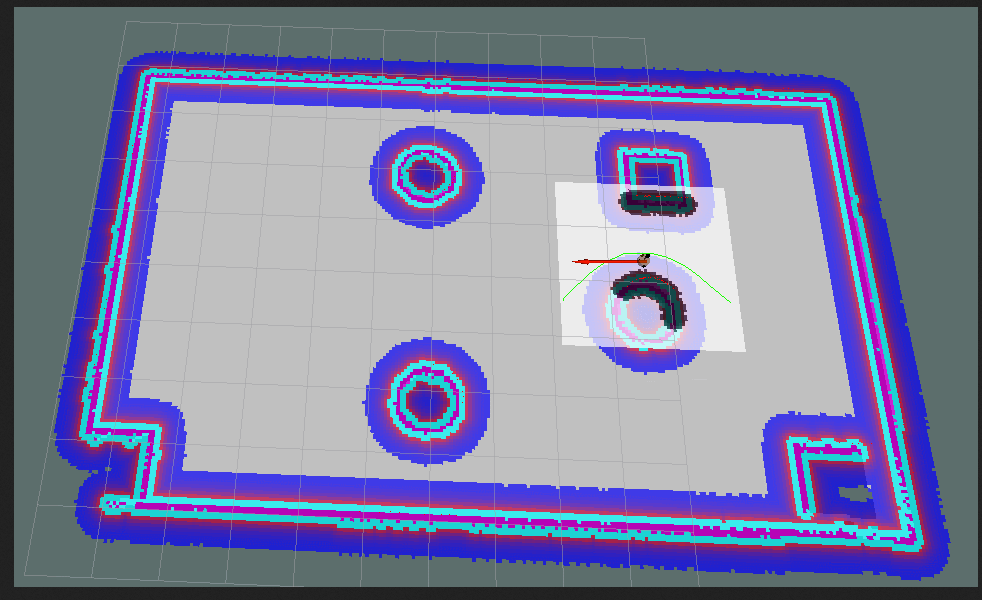
\includegraphics[width=.7\textwidth]{navigation_demo.png}
  \caption{仿真环境下的导航实现}
  \label{fig:navigation_demo}
\end{figure}

演示2: DIY的机器人.

\begin{figure}[!ht]
  \centering
  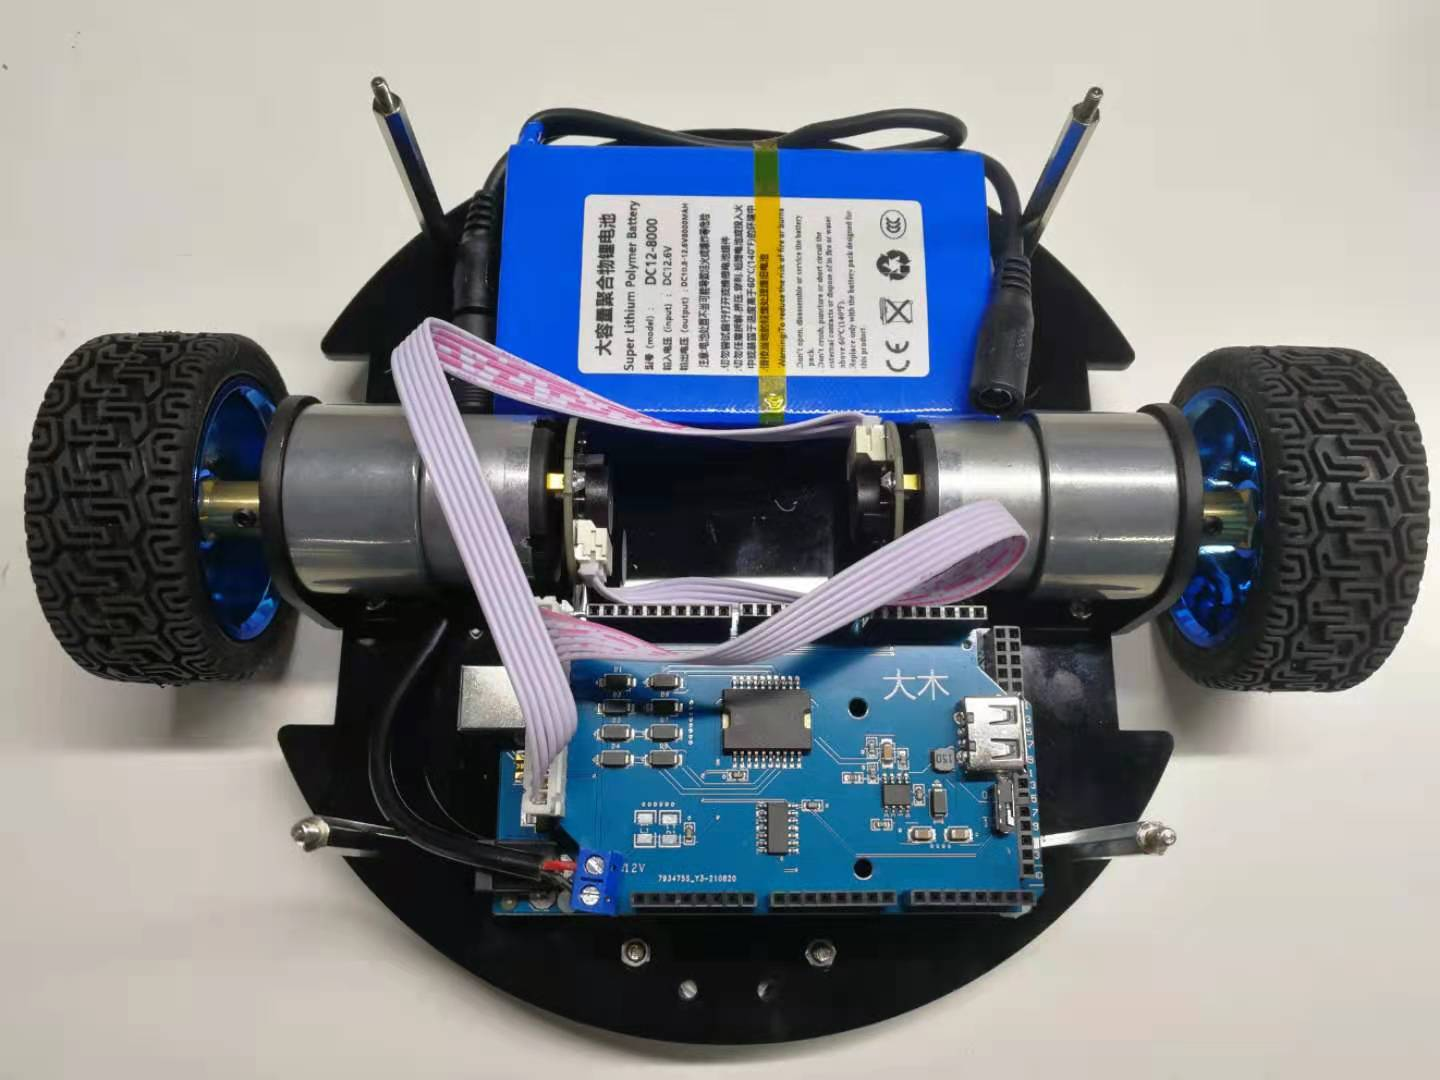
\includegraphics[width=.5\textwidth]{robot_chassis_front.jpg}
  \caption{机器人底盘正面}
  \label{fig:robot_chassis_front_}
\end{figure}

\begin{figure}[!ht]
  \centering
  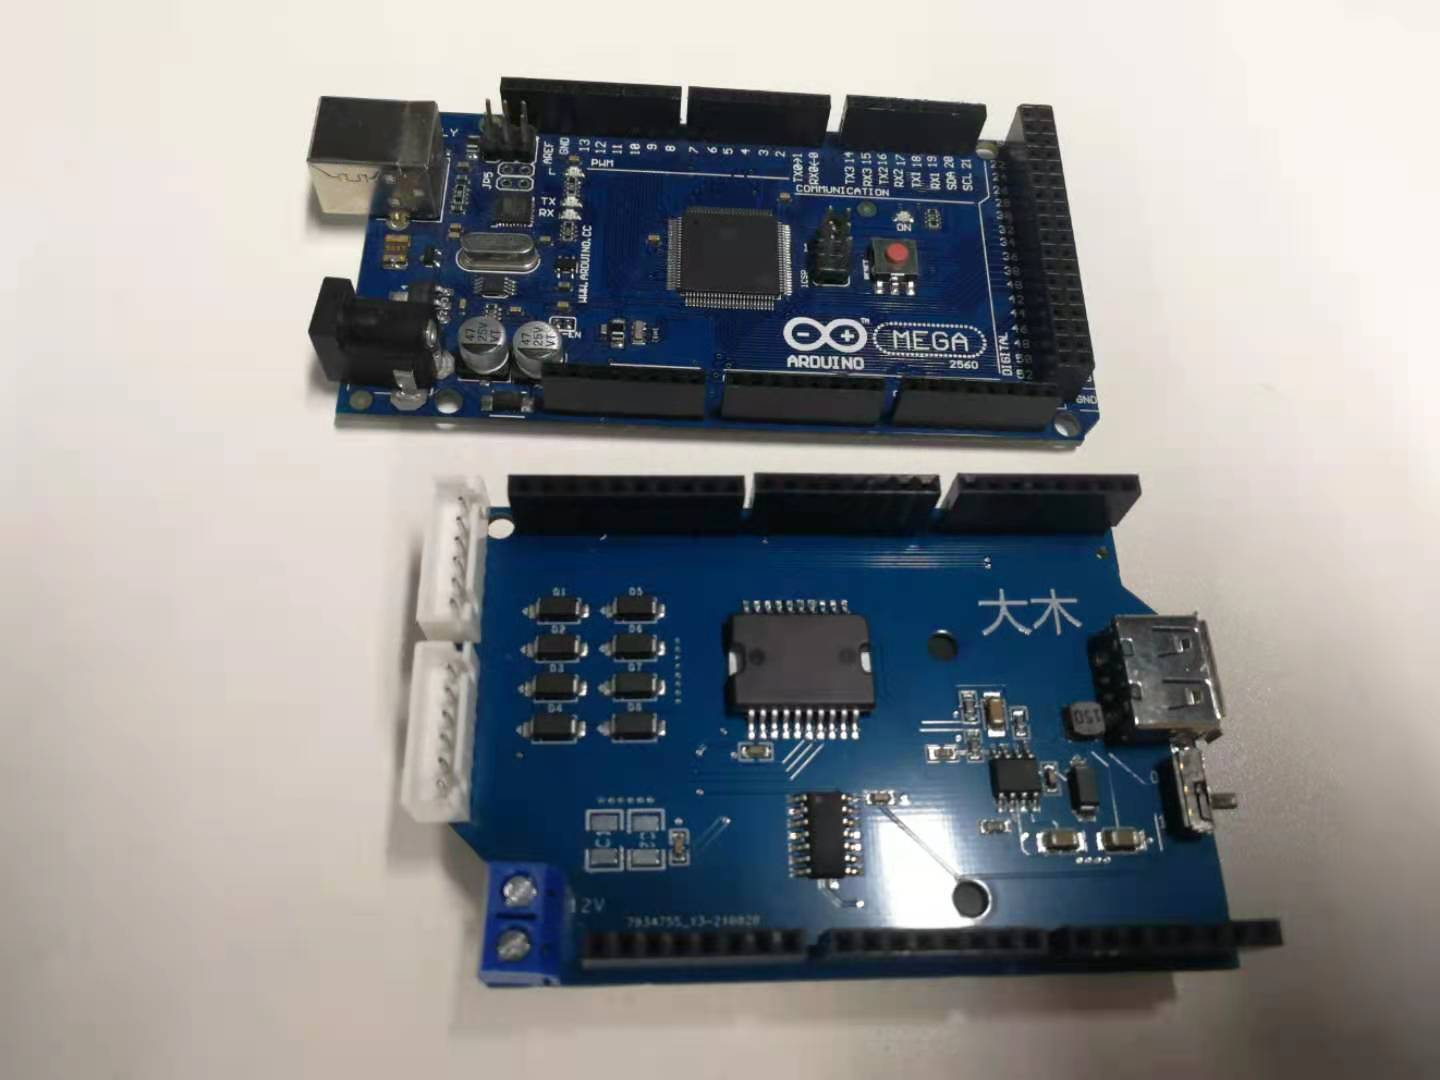
\includegraphics[width=.5\textwidth]{robot_arduino_board.jpg}
  \caption{机器人Arduino 与电机驱动板}
  \label{fig:robot_arduino_board_}
\end{figure}

\begin{figure}[!ht]
  \centering
  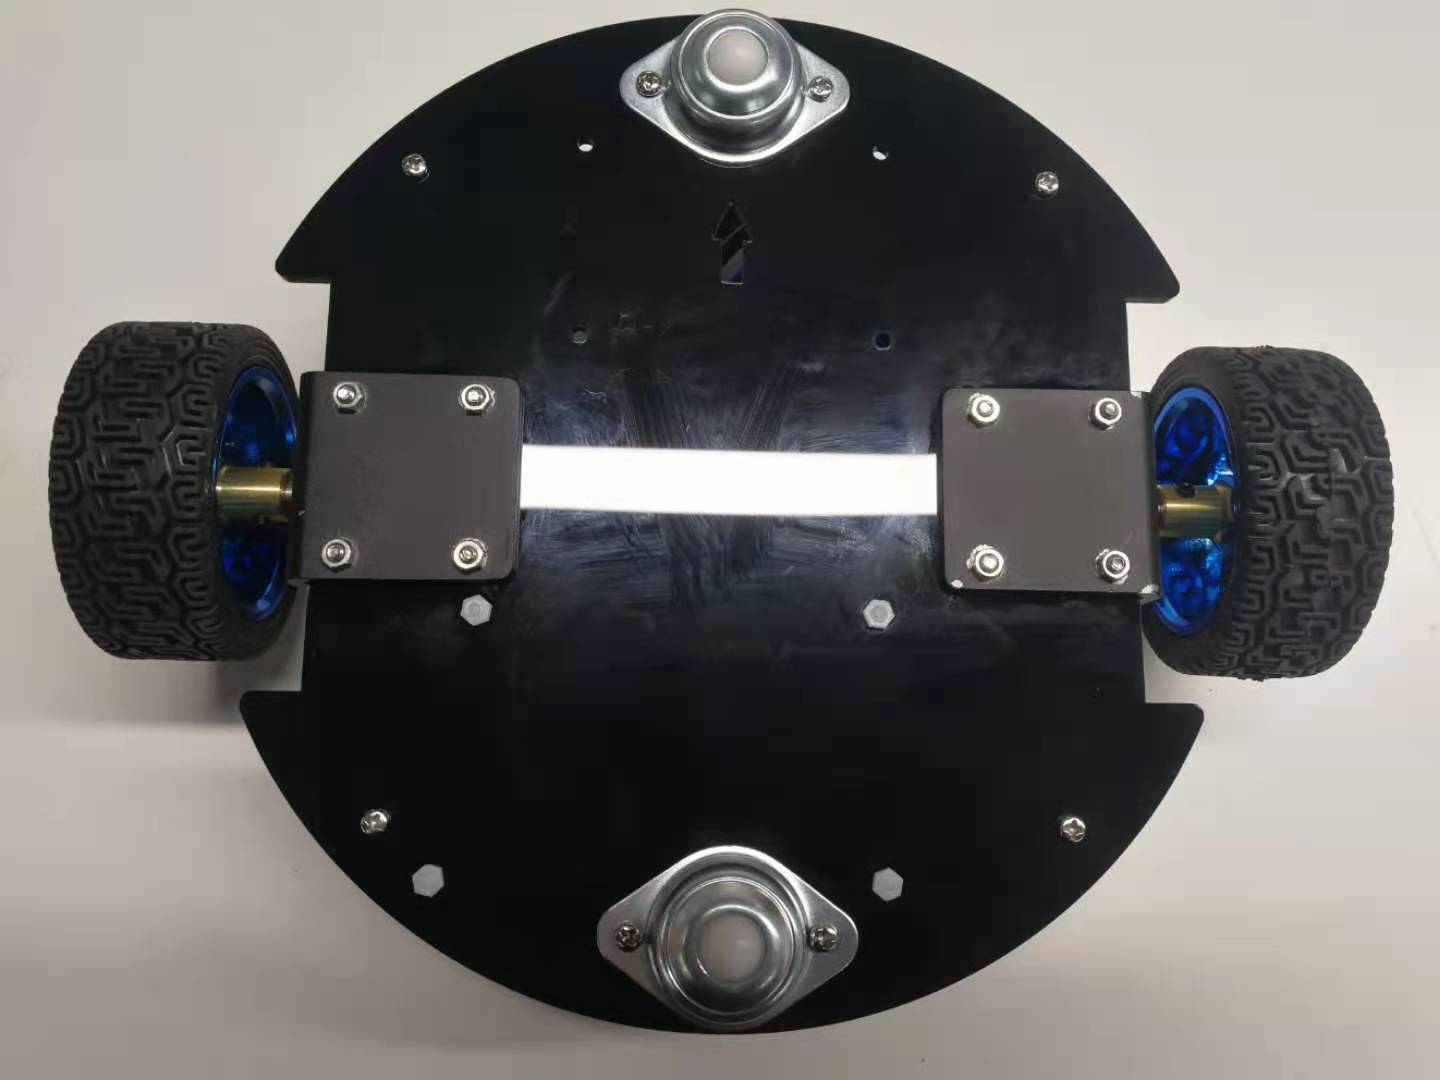
\includegraphics[width=.5\textwidth]{robot_chassis_back.jpg}
  \caption{机器人底盘背面}
  \label{fig:robot_chassis_back_}
\end{figure}

演示3: \href{https://www.bilibili.com/video/BV15z4y1672p}{机器人SLAM}.

演示4: \href{https://www.bilibili.com/video/BV1j5411n7Nc}{机器人多点导航}.

演示5: \href{https://www.bilibili.com/video/BV1bx411E7SC}{ROS模拟器}.

\tableofcontents

\listoffigures

\listoftables

\mainmatter

\chapter{ROS概述与环境搭建}

学习是一个循序渐进的过程, 具体到计算机领域的软件开发层面, 每当接触一个新的知识模块时, 按照一般的步骤, 我们会先去了解该模块的相关概念, 然后再安装官方软件包, 接下来再搭建其集成的开发环境等等. 这些准备工作完毕之后, 才算是叩开了新领域的大门. 学习 ROS, 我们也是遵循这一流程, 本章作为 ROS 体系的开篇主要内容如下:

\begin{itemize}
  \item ROS的相关概念;
  \item 怎样安装ROS;
  \item 如何搭建 ROS 的集成开发环境.
\end{itemize}

该章内容学习完毕预期达成的目标如下:

\begin{itemize}
  \item 了解 ROS 概念、设计目标以及发展历程;
  \item 能够独立安装并运行 ROS;
  \item 能够使用 C++ 或 Python 实现 ROS 版本的 HelloWorld;
  \item 能够搭建 ROS 的集成开发环境;
  \item 了解 ROS 架构设计.
\end{itemize}

\section{ROS简介}

\subsection{ROS概念}

ROS 全称: Robot Operating System (机器人操作系统).

\begin{itemize}
  \item ROS是适用于机器人的开源元操作系统;
  \item ROS集成了大量的工具, 库, 协议, 提供类似 OS 所提供的功能, 简化对机器人的控制;
  \item 还提供了用于在多台计算机上获取, 构建, 编写和运行代码的工具和库, ROS在某些方面类似于机器人框架;
  \item ROS设计者将 ROS 表述为 ROS = Plumbing + Tools + Capabilities + Ecosystem, 即 ROS 是通讯机制、工具软件包、机器人高层技能以及机器人生态系统的集合体.
\end{itemize}

\begin{figure}[!ht]
  \centering
  
\includegraphics[width=.9\textwidth]{ros_intro.png}
  \caption{ROS架构简介}
  \label{fig:ros_intro}
\end{figure}

\subsection{ROS设计目标}

机器人开发的分工思想, 实现了不同研发团队间的共享和协作, 提升了机器人的研发效率, 为了服务分工, ROS 主要设计了如下目标: 

\begin{itemize}
  \item 代码复用: ROS 的目标不是成为具有最多功能的框架, ROS 的主要目标是支持机器人技术研发中的代码重用.

  \item 分布式: ROS 是进程 (也称为 Nodes) 的分布式框架, ROS 中的进程可分布于不同主机, 不同主机协同工作, 从而分散计算压力

  \item 松耦合: ROS 中功能模块封装于独立的功能包或元功能包, 便于分享, 功能包内的模块以节点为单位运行, 以 ROS 标准的 IO 作为接口, 开发者不需要关注模块内部实现, 只要了解接口规则就能实现复用, 实现了模块间点对点的松耦合连接

  \item 精简: ROS 被设计为尽可能精简, 以便为 ROS 编写的代码可以与其他机器人软件框架一起使用. ROS 易于与其他机器人软件框架集成: ROS 已与 OpenRAVE, Orocos 和 Player 集成.

  \item 语言独立性: 包括 Java, C++, Python 等. 为了支持更多应用开发和移植, ROS 设计为一种语言弱相关的框架结构, 使用简洁, 中立的定义语言描述模块间的消息接口, 在编译中再产生所使用语言的目标文件, 为消息交互提供支持, 同时允许消息接口的嵌套使用

  \item 易于测试: ROS 具有称为 \verb|rostest| 的内置单元/集成测试框架, 可轻松安装和拆卸测试工具.

  \item 大型应用: ROS 适用于大型运行时系统和大型开发流程.

  \item 丰富的组件化工具包: ROS 可采用组件化方式集成一些工具和软件到系统中并作为一个组件直接使用, 如 RViz (3D可视化工具), 开发者根据 ROS 定义的接口在其中显示机器人模型等, 组件还包括仿真环境和消息查看工具等.

  \item 免费且开源: 开发者众多, 功能包多.
\end{itemize}

\subsection{ROS发展历程}

ROS 是一个由来已久、贡献者众多的大型软件项目. 在 ROS 诞生之前, 很多学者认为, 机器人研究需要一个开放式的协作框架, 并且已经有不少类似的项目致力于实现这样的框架. 在这些工作中, 斯坦福大学在2000年年中开展了一系列相关研究项目, 如斯坦福人工智能机器人 (STandford AI Robot, STAIR) 项目、个人机器人 (Personal Robots, PR) 项目等, 在上述项目中, 在研究具有代表性、集成式人工智能系统的过程中, 创立了用于室内场景的高灵活性、动态软件系统, 其可以用于机器人学研究.

2007 年, 柳树车库 (Willow Garage) 提供了大量资源, 用于将斯坦福大学机器人项目中的软件系统进行扩展与完善, 同时, 在无数研究人员的共同努力下, ROS 的核心思想和基本软件包逐渐得到完善.

ROS 的发行版本 (ROS distribution) 指 ROS 软件包的版本, 其与 Linux 的发行版本 (如 Ubuntu) 的概念类似. 推出 ROS 发行版本的目的在于使开发人员可以使用相对稳定的代码库, 直到其准备好将所有内容进行版本升级为止. 因此, 每个发行版本推出后, ROS 开发者通常仅对这一版本的bug进行修复, 同时提供少量针对核心软件包的改进.

版本特点: 按照英文字母顺序命名, ROS 目前已经发布了ROS1 的终极版本: noetic, 并建议后期过渡至 ROS2 版本. noetic 版本之前默认使用的是 Python2, noetic 支持 Python3.

建议版本: noetic 或 melodic 或 kinetic.

\begin{figure}[!ht]
  \centering
  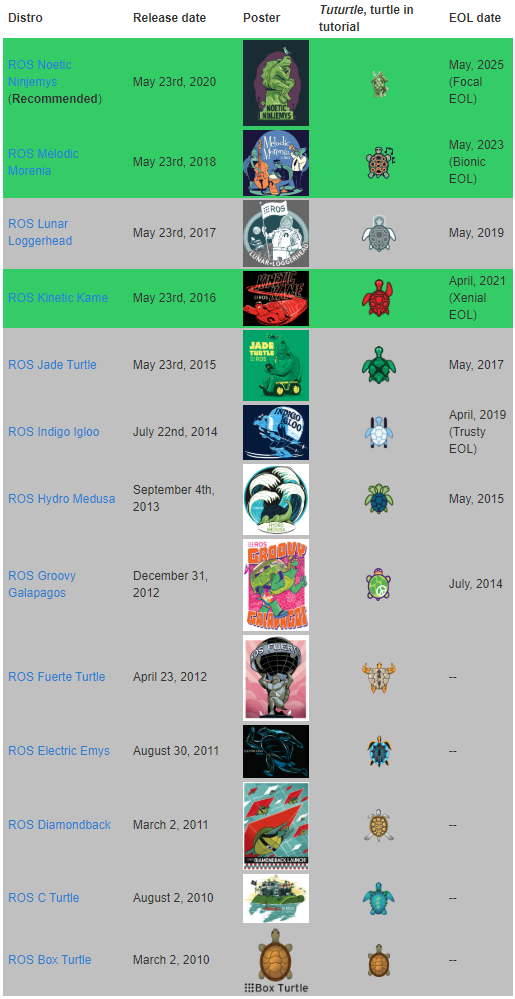
\includegraphics[width=.55\textwidth]{ros_versions.png}
  \caption{ROS不同版本}
  \label{fig:ros_versions}
\end{figure}

\section{ROS安装}

\subsection{安装虚拟机软件}

参考 \href{http://www.autolabor.com.cn/book/ROSTutorials/chapter1/12-roskai-fa-gong-ju-an-zhuang/121-an-zhuang-xu-ni-ji-ruan-jian.html}{安装虚拟机软件}.

\subsection{虚拟一台主机}

参考 \href{http://www.autolabor.com.cn/book/ROSTutorials/chapter1/12-roskai-fa-gong-ju-an-zhuang/122-xu-ni-yi-tai-zhu-ji.html}{虚拟一台主机}.

\subsection{安装Ubuntu}

参考 \href{http://www.autolabor.com.cn/book/ROSTutorials/chapter1/12-roskai-fa-gong-ju-an-zhuang/123-an-zhuang-ubuntu.html}{安装Ubuntu}.

\subsection{安装ROS}

Ubuntu 安装完毕后, 就可以安装 ROS 操作系统了, 大致步骤如下:

\begin{enumerate}
  \item 设置安装源;
  \item 设置 key;
  \item 配置 Ubuntu 的软件和更新, 安装;
  \item 配置环境变量.
\end{enumerate}

1. 设置安装源:

官方默认安装源:

\begin{bash}
  sudo sh -c 'echo "deb http://packages.ros.org/ros/ubuntu $(lsb_release -sc) main" > /etc/apt/sources.list.d/ros-latest.list'
\end{bash}

或来自国内清华的安装源:

\begin{bash}
  sudo sh -c '. /etc/lsb-release && echo "deb http://mirrors.tuna.tsinghua.edu.cn/ros/ubuntu/ `lsb_release -cs` main" > /etc/apt/sources.list.d/ros-latest.list'
\end{bash}

或来自国内中科大的安装源:

\begin{bash}
  sudo sh -c '. /etc/lsb-release && echo "deb http://mirrors.ustc.edu.cn/ros/ubuntu/ `lsb_release -cs` main" > /etc/apt/sources.list.d/ros-latest.list'
\end{bash}

PS: 回车后, 可能需要输入管理员密码; 建议使用国内资源, 安装速度更快.

2. 设置 key:

\begin{bash}
  sudo apt-key adv --keyserver 'hkp://keyserver.ubuntu.com:80' --recv-key C1CF6E31E6BADE8868B172B4F42ED6FBAB17C654
\end{bash}

3. 安装

首先需要更新 apt (以前是 apt-get, 官方建议使用 apt 而非 apt-get), apt 是用于从互联网仓库搜索、安装、升级、卸载软件或操作系统的工具.

\begin{bash}
  sudo apt update
\end{bash}

等待. 然后, 再安装所需类型的 ROS: ROS 多个类型: Desktop-Full、Desktop、ROS-Base. 这里介绍较为常用的Desktop-Full (官方推荐) 安装: ROS, rqt, rviz, robot-generic libraries, 2D/3D simulators, navigation and 2D/3D perception

\begin{bash}
  sudo apt install ros-noetic-desktop-full
\end{bash}

4. 配置环境变量

配置环境变量, 方便在任意终端中使用 ROS.

\begin{bash}
  echo "source /opt/ros/noetic/setup.bash" >> ~/.bashrc
  source ~/.bashrc
\end{bash}

卸载: 如果需要卸载 ROS 可以调用如下命令:

\begin{bash}
  sudo apt remove ros-noetic-*
\end{bash}

注意: 在 ROS 版本 noetic 中无需构建软件包的依赖关系, 没有 \verb|rosdep| 的相关安装与配置.

\subsection{测试ROS}

ROS 内置了一些小程序, 可以通过运行这些小程序以检测 ROS 环境是否可以正常运行:

\begin{itemize}
  \item 首先启动三个命令行 (Ctrl + Alt + T);

  \item 命令行1键入:
  \begin{bash}
    roscore
  \end{bash}

  \item 命令行2键入: (此时会弹出图形化界面)
  \begin{bash}
    rosrun turtlesim turtlesim_node
  \end{bash}

  \item 命令行3键入: (在3中可以通过上下左右控制2中乌龟的运动)
  \begin{bash}
    rosrun turtlesim turtle_teleop_key
  \end{bash}
\end{itemize}

最终结果如下所示. 注意: 光标必须聚焦在键盘控制窗口, 否则无法控制乌龟运动.

\begin{figure}[!ht]
  \centering
  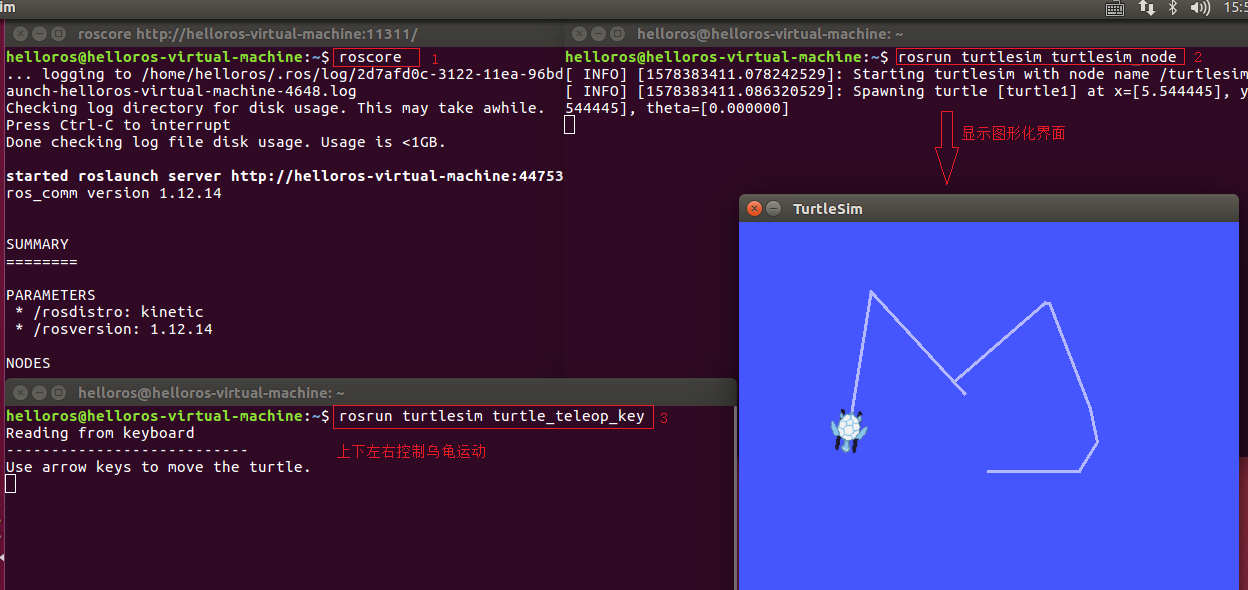
\includegraphics[width=.9\textwidth]{ros_test_turtlesim.png}
  \caption{ROS测试示例}
  \label{fig:ros_test_turtlesim}
\end{figure}

\subsection{其他 ROS 版本安装}

我们的教程采用的是 ROS 的最新版本 noetic, 不过 noetic 较之于之前的 ROS 版本变动较大且部分功能包还未更新, 因此如果有需要 (比如到后期实践阶段, 由于部分重要的功能包还未更新, 需要 ROS 降级), 也会安装之前版本的 ROS, 在此, 建议选用的版本是 melodic 或 kinetic.

接下来, 就以 melodic 为例演示 ROS 历史版本安装 (当然先要准备与melodic对应的Ubuntu18.04): \href{http://www.autolabor.com.cn/book/ROSTutorials/chapter1/12-roskai-fa-gong-ju-an-zhuang/127-zi-65993a-qi-ta-ros-ban-ben-an-zhuang.html}{其他 ROS 版本安装}.

\section{ROS快速体验}

\subsection{HelloWorld实现简介}

ROS 中涉及的编程语言以 C++ 和 Python 为主, ROS 中的大多数程序两者都可以实现, 在本系列教程中, 每一个案例也都会分别使用 C++ 和 Python 两种方案演示, 大家可以根据自身情况选择合适的实现方案.

ROS 中的程序即便使用不同的编程语言, 实现流程也大致类似, 以当前 HelloWorld 程序为例, 实现流程大致如下: 

\begin{enumerate}
  \item 先创建一个工作空间; 
  \item 再创建一个功能包; 
  \item 编辑源文件; 
  \item 编辑配置文件; 
  \item 编译并执行.
\end{enumerate}

上述流程中, C++ 和 Python 只是在步骤3和步骤4的实现细节上存在差异, 其他流程基本一致. 本节先实现 C++ 和 Python 程序编写的通用部分步骤1与步骤2, 1.3.2节和1.3.3节再分别使用 C++ 和 Python 编写HelloWorld.

1. 创建工作空间并初始化

\begin{bash}
  mkdir -p 自定义空间名称/src
  cd 自定义空间名称
  catkin_make
\end{bash}

上述命令, 首先会创建一个工作空间以及一个 \verb|src| 子目录, 然后再进入工作空间调用 \verb|catkin_make| 命令编译.

2. 进入 \verb|src| 创建 ROS 包并添加依赖

\begin{bash}
  cd src
  catkin_create_pkg your_ros_package roscpp rospy std_msgs
\end{bash}

上述命令会在工作空间下生成一个功能包, 该功能包依赖 \verb|roscpp|、\verb|rospy| 与 \verb|std_msgs|, 其中 \verb|roscpp| 是使用 C++ 实现的库, 而 \verb|rospy| 则是使用 Python 实现的库, \verb|std_msgs| 是标准消息库, 创建 ROS 功能包时, 一般都会依赖这三个库实现.

注意: 在 ROS 中, 虽然实现同一功能时, C++ 和 Python 可以互换, 但是具体选择哪种语言, 需要视需求而定, 因为两种语言相较而言: C++ 运行效率高但是编码效率低, 而 Python 则反之, 基于二者互补的特点, ROS 设计者分别设计了 \verb|roscpp| 与 \verb|rospy| 库, 前者旨在成为 ROS 的高性能库, 而后者则一般用于对性能无要求的场景, 旨在提高开发效率.

\subsection{HelloWorld 实现 (C++)}

本节内容基于1.3.1, 假设你已经创建了 ROS 的工作空间, 并且创建了 ROS 的功能包, 那么就可以进入核心步骤了, 使用 C++ 编写程序实现: 

1. 进入 ROS 包的 \verb|src| 目录编辑源文件

\begin{bash}
  cd 自定义的包
\end{bash}

C++ 源码实现: (文件名自定义)

\begin{cpp}
  #include "ros/ros.h"

  int main(int argc, char *argv[])
  {
      // 执行 ros 节点初始化
      ros::init(argc,argv,"hello");
      // 创建 ros 节点句柄 (非必须)
      ros::NodeHandle n;
      // 控制台输出 hello world
      ROS_INFO("hello world!");

      return 0;
  }
\end{cpp}

2. 编辑 ROS 包下的 \verb|Cmakelists.txt| 文件

\begin{bash}
  add_executable(步骤3的源文件名
    src/步骤3的源文件名.cpp
  )
  target_link_libraries(步骤3的源文件名
    ${catkin_LIBRARIES}
  )
\end{bash}

3. 进入工作空间目录并编译

\begin{bash}
  cd 自定义空间名称
  catkin_make
\end{bash}

生成 build devel ....

4. 执行

先启动命令行1: 

\begin{bash}
  roscore
\end{bash}

再启动命令行2: 

\begin{bash}
  cd 工作空间
  source ./devel/setup.bash
  rosrun 包名 C++节点
\end{bash}

命令行输出: \verb|HelloWorld!|.

PS: \verb|source ~/工作空间/devel/setup.bash| 可以添加进 \verb|.bashrc| 文件, 使用上更方便.

添加方式1: 直接使用 \verb|gedit| 或 \verb|vi| 编辑 \verb|.bashrc| 文件, 最后添加该内容.

添加方式2:

\begin{bash}
  echo "source ~/工作空间/devel/setup.bash" >> ~/.bashrc
\end{bash}

\subsection{HelloWorld 实现 (Python)}

本节内容基于1.3.1, 假设你已经创建了 ROS 的工作空间, 并且创建了 ROS 的功能包, 那么就可以进入核心步骤了, 使用 Python 编写程序实现:

1. 进入 ROS 包添加 scripts 目录并编辑 Python 文件:

\begin{bash}
  cd ros包
  mkdir scripts
\end{bash}

新建 Python 文件: (文件名自定义)

\begin{python}
  #! /usr/bin/env python

  """
      Python 版 HelloWorld

  """
  import rospy

  if __name__ == "__main__":
      rospy.init_node("Hello")
      rospy.loginfo("Hello World!!!!")
\end{python}

2. 为 Python 文件添加可执行权限

\begin{bash}
  chmod +x 自定义文件名.py
\end{bash}

3. 编辑 ROS 包下的 \verb|CmakeLists.txt| 文件

\begin{bash}
  catkin_install_python(PROGRAMS scripts/自定义文件名.py
    DESTINATION ${CATKIN_PACKAGE_BIN_DESTINATION}
  )
\end{bash}

4. 进入工作空间目录并编译

\begin{bash}
  cd 自定义空间名称
  catkin_make
\end{bash}

5. 进入工作空间目录并执行

先启动命令行1:

\begin{bash}
  roscore
\end{bash}

再启动命令行2:

\begin{bash}
  cd 工作空间
  source ./devel/setup.bash
  rosrun 包名 自定义文件名.py
\end{bash}

输出结果: \verb|Hello World!!!!|

\section{ROS集成开发环境搭建}

和大多数开发环境一样, 理论上, 在 ROS 中, 只需要记事本就可以编写基本的 ROS 程序, 但是工欲善其事必先利其器, 为了提高开发效率, 可以先安装集成开发工具和使用方便的工具: 终端、IDE 等等.

\subsection{安装终端}

在 ROS 中, 需要频繁的使用到终端, 且可能需要同时开启多个窗口, 推荐一款较为好用的终端: Terminator. 效果如下:

\begin{figure}[!ht]
  \centering
  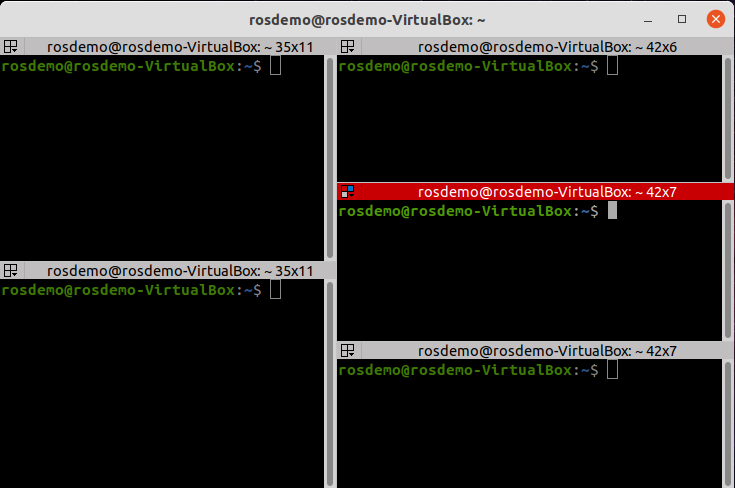
\includegraphics[width=.9\textwidth]{terminator_illustration.png}
  \caption{Terminator 效果}
  \label{fig:ternimal_illustration}
\end{figure}

1. 安装

\begin{bash}
  sudo apt install terminator
\end{bash}

2. 添加到收藏夹

显示应用程序 $\rightarrow$ 搜索 terminator $\rightarrow$ 右击 选择 \verb|添加到收藏夹|.

3. Terminator 常用快捷键

第一部份: 关于在同一个标签内的操作:

\begin{bash}
  Alt+Up                          // 移动到上面的终端
  Alt+Down                        // 移动到下面的终端
  Alt+Left                        // 移动到左边的终端
  Alt+Right                       // 移动到右边的终端
  Ctrl+Shift+O                    // 水平分割终端
  Ctrl+Shift+E                    // 垂直分割终端
  Ctrl+Shift+Right                // 在垂直分割的终端中将分割条向右移动
  Ctrl+Shift+Left                 // 在垂直分割的终端中将分割条向左移动
  Ctrl+Shift+Up                   // 在水平分割的终端中将分割条向上移动
  Ctrl+Shift+Down                 // 在水平分割的终端中将分割条向下移动
  Ctrl+Shift+S                    // 隐藏/显示滚动条
  Ctrl+Shift+F                    // 搜索
  Ctrl+Shift+C                    // 复制选中的内容到剪贴板
  Ctrl+Shift+V                    // 粘贴剪贴板的内容到此处
  Ctrl+Shift+W                    // 关闭当前终端
  Ctrl+Shift+Q                    // 退出当前窗口, 当前窗口的所有终端都将被关闭
  Ctrl+Shift+X                    // 最大化显示当前终端
  Ctrl+Shift+Z                    // 最大化显示当前终端并使字体放大
  Ctrl+Shift+N or Ctrl+Tab        // 移动到下一个终端
  Ctrl+Shift+P or Ctrl+Shift+Tab  // Crtl+Shift+Tab 移动到之前的一个终端
\end{bash}

第二部份: 有关各个标签之间的操作:

\begin{bash}
  F11                             // 全屏开关
  Ctrl+Shift+T                    // 打开一个新的标签
  Ctrl+PageDown                   // 移动到下一个标签
  Ctrl+PageUp                     // 移动到上一个标签
  Ctrl+Shift+PageDown             // 将当前标签与其后一个标签交换位置
  Ctrl+Shift+PageUp               // 将当前标签与其前一个标签交换位置
  Ctrl+Plus (+)                   // 增大字体
  Ctrl+Minus (-)                  // 减小字体
  Ctrl+Zero (0)                   // 恢复字体到原始大小
  Ctrl+Shift+R                    // 重置终端状态
  Ctrl+Shift+G                    // 重置终端状态并clear屏幕
  Super+g                         // 绑定所有的终端, 以便向一个输入能够输入到所有的终端
  Super+Shift+G                   // 解除绑定
  Super+t                         // 绑定当前标签的所有终端, 向一个终端输入的内容会自动输入到其他终端
  Super+Shift+T                   // 解除绑定
  Ctrl+Shift+I                    // 打开一个窗口, 新窗口与原来的窗口使用同一个进程
  Super+i                         // 打开一个新窗口, 新窗口与原来的窗口使用不同的进程
\end{bash}

\subsection{安装VSCode}

VSCode 全称 Visual Studio Code, 是微软出的一款轻量级代码编辑器, 免费、开源而且功能强大. 它支持几乎所有主流的程序语言的语法高亮、智能代码补全、自定义热键、括号匹配、代码片段、代码对比 Diff、GIT 等特性, 支持插件扩展, 并针对网页开发和云端应用开发做了优化. 软件跨平台支持 Win、Mac 以及 Linux.

1. 下载

VSCode\href{https://code.visualstudio.com/docs?start=true}{下载}, 历史版本 \href{https://code.visualstudio.com/updates}{下载链接}.

2. VSCode 安装与卸载

2.1 安装

方式1: 双击安装即可 (或右击选择安装).

方式2:

\begin{bash}
  sudo dpkg -i xxxx.deb
\end{bash}

2.2 卸载

\begin{bash}
  sudo dpkg --purge  code
\end{bash}

3. VSCode 集成 ROS 插件

使用 VSCode 开发 ROS 程序, 需要先安装一些插件, 常用插件如下:

4. VSCode 基本配置

4.1 创建 ROS 工作空间

\begin{bash}
  mkdir -p xxx_ws/src
  cd xxx_ws
  catkin_make
\end{bash}

4.2 启动 VSCode

进入 \verb|xxx_ws| 启动 VSCode:

\begin{bash}
  cd xxx_ws
  code .
\end{bash}

4.3 VSCode 中编译 ros

快捷键 Ctrl + Shift + B 调用编译, 选择: \verb|catkin_make:build|. 可以点击配置设置为默认, 修改 \verb|.vscode/tasks.json| 文件:

\begin{bash}
  {
  // 有关 tasks.json 格式的文档, 请参见
      // https://go.microsoft.com/fwlink/?LinkId=733558
      "version": "2.0.0",
      "tasks": [
          {
              "label": "catkin_make:debug", // 代表提示的描述性信息
              "type": "shell",  // 可以选择shell或者process, 如果是shell代码是在shell里面运行一个命令, 如果是process代表作为一个进程来运行
              "command": "catkin_make", // 这个是我们需要运行的命令
              "args": [], // 如果需要在命令后面加一些后缀, 可以写在这里, 比如-DCATKIN_WHITELIST_PACKAGES=“pac1;pac2”
              "group": {"kind":"build","isDefault":true},
              "presentation": {
                  "reveal": "always" // 可选always或者silence, 代表是否输出信息
              },
              "problemMatcher": "$msCompile"
          }
      ]
  }
\end{bash}

4.4 创建 ROS 功能包

选定 \verb|src| 右击: \verb|create catkin package|.

设置包名 添加依赖

4.5 C++ 实现

在功能包的 \verb|src| 下新建 C++ 文件:

\begin{cpp}
  /**
   *  控制台输出 Hello VSCode !!!
   */

  #include "ros/ros.h"

  int main(int argc, char *argv[])
  {
      setlocale(LC_ALL,"");
      // 执行节点初始化
      ros::init(argc,argv,"HelloVSCode");

      // 输出日志
      ROS_INFO("Hello VSCode!!!");
      return 0;
  }
\end{cpp}

PS1: 如果没有代码提示, 修改 \verb|.vscode/c_cpp_properties.json|, 设置:

\begin{xml}
  "cppStandard": "c++17"
\end{xml}

PS2: \verb|main| 函数的参数不可以被 \verb|const| 修饰.

PS3: 当 \verb|ROS_INFO| 终端输出有中文时, 会出现乱码: \verb|INFO: ????????????????|.

解决办法: 在函数开头加入下面代码的任意一句:

\begin{cpp}
  setlocale(LC_CTYPE, "zh_CN.utf8");
  setlocale(LC_ALL, "");
\end{cpp}

4.6 Python 实现

在 \verb|功能包/| 下新建 \verb|scripts| 文件夹, 添加 Python 文件, 并添加可执行权限.

\begin{python}
  #! /usr/bin/env python
  """
      Python 版本的 Hello VSCode, 执行在控制台输出 Hello VScode
      实现:
      1. 导包
      2. 初始化 ROS 节点
      3. 日志输出 HelloWorld
  """

  import rospy # 1. 导包

  if __name__ == "__main__":
      rospy.init_node("Hello_Vscode_p")  # 2. 初始化 ROS 节点
      rospy.loginfo("Hello VSCode, 我是 Python ....")  # 3. 日志输出 HelloWorld
\end{python}

4.7 配置 \verb|CMakeLists.txt|

C++ 配置:

\begin{bash}
  add_executable(节点名称
    src/C++源文件名.cpp
  )
  target_link_libraries(节点名称
    ${catkin_LIBRARIES}
  )
\end{bash}

Python 配置:

\begin{bash}
  catkin_install_python(PROGRAMS scripts/自定义文件名.py
    DESTINATION ${CATKIN_PACKAGE_BIN_DESTINATION}
  )
\end{bash}

4.8 编译执行

编译: Ctrl + Shift + B.

执行: 和之前一致, 只是可以在 VSCode 中添加终端, 首先执行:

\begin{bash}
  source ./devel/setup.bash
\end{bash}

PS: 如果不编译直接执行 Python 文件, 会抛出异常.

1. 第一行解释器声明, 可以使用绝对路径定位到 python3 的安装路径 

\begin{bash}
  #! /usr/bin/python3
\end{bash}

但是不建议.

2. 建议使用 \verb|#!/usr/bin/env python| 但是会抛出异常 : \verb|/usr/bin/env: python|: 没有那个文件或目录.

3. 解决1: \verb|#!/usr/bin/env python3| 直接使用 python3 但存在问题: 不兼容之前的 ROS 相关 Python 实现.

4. 解决2: 创建一个链接符号到 Python 命令:

\begin{bash}
  sudo ln -s /usr/bin/python3 /usr/bin/python
\end{bash}

\subsection{launch文件演示}

1. 需求: 一个程序中可能需要启动多个节点, 比如: ROS 内置的小乌龟案例, 如果要控制乌龟运动, 要启动多个窗口, 分别启动 \verb|roscore|、乌龟界面节点、键盘控制节点. 如果每次都调用 \verb|rosrun| 逐一启动, 显然效率低下, 如何优化? 官方给出的优化策略是使用 launch 文件, 可以一次性启动多个 ROS 节点.

2. 实现

\begin{itemize}
  \item 选定功能包右击 $\rightarrow$ 添加 launch 文件夹;

  \item 选定 launch 文件夹右击 $\rightarrow$ 添加 launch 文件;

  \item 编辑 launch 文件内容:

  \begin{xml}
    <launch>
        <node pkg="helloworld" type="demo_hello" name="hello" output="screen" />
        <node pkg="turtlesim" type="turtlesim_node" name="t1"/>
        <node pkg="turtlesim" type="turtle_teleop_key" name="key1" />
    </launch>
  \end{xml}

  \begin{itemize}
    \item \verb|node|: 包含的某个节点;
    \item \verb|pkg|: 功能包;
    \item \verb|type|: 被运行的节点文件;
    \item \verb|name|: 为节点命名;
    \item \verb|output|: 设置日志的输出目标;
  \end{itemize}

  \item 运行 launch 文件;
  
  \begin{bash}
    roslaunch 包名 launch文件名
  \end{bash}

  运行结果: 一次性启动了多个节点.
\end{itemize}

\section{ROS架构}

\subsection{ROS文件系统}

ROS 文件系统级指的是在硬盘上 ROS 源代码的组织形式, 其结构大致可以如下图所示: 

\begin{figure}[!ht]
  \centering
  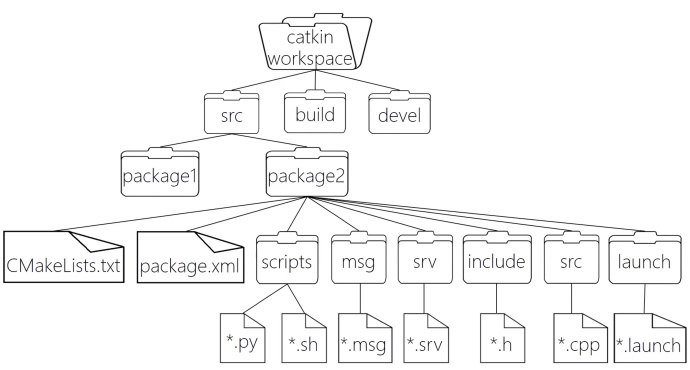
\includegraphics[width=.8\textwidth]{ros_file_system.jpg}
  \caption{ROS文件系统}
  \label{fig:ros_file_system}
\end{figure}

\begin{bash}
  WorkSpace --- 自定义的工作空间

    |--- build: 编译空间, 用于存放 CMake 和 catkin 的缓存信息、配置信息和其他中间文件.

    |--- devel: 开发空间, 用于存放编译后生成的目标文件, 包括头文件、动态&静态链接库、可执行文件等.

    |--- src: 源码

        |-- package: 功能包 (ROS基本单元)包含多个节点、库与配置文件, 包名所有字母小写, 只能由字母、数字与下划线组成

            |-- CMakeLists.txt 配置编译规则, 比如源文件、依赖项、目标文件

            |-- package.xml 包信息, 比如:包名、版本、作者、依赖项等等 (以前版本是 manifest.xml)

            |-- scripts 存储python文件

            |-- src 存储C++源文件

            |-- include 头文件

            |-- msg 消息通信格式文件

            |-- srv 服务通信格式文件

            |-- action 动作格式文件

            |-- launch 可一次性运行多个节点 

            |-- config 配置信息

        |-- CMakeLists.txt: 编译的基本配置
\end{bash}

ROS 文件系统中部分目录和文件前面编程中已经有所涉及, 比如功能包的创建、\verb|src| 目录下 C++ 文件的编写、\verb|scripts| 目录下python文件的编写、\verb|launch| 目录下launch文件的编写, 并且也配置了 \verb|package.xml| 与 \verb|CMakeLists.txt| 文件. 其他目录下的内容后面教程将会再行介绍, 当前我们主要介绍: \verb|package.xml| 与 \verb|CMakeLists.txt| 这两个配置文件.

1. \verb|package.xml|

该文件定义有关软件包的属性, 例如软件包名称, 版本号, 作者, 维护者以及对其他 catkin 软件包的依赖性. 该概念类似于旧版 \verb|rosbuild| 构建系统中使用的 \verb|manifest.xml| 文件.

\begin{xml}
  <?xml version="1.0"?>
  <!-- 格式: 以前是 1, 推荐使用格式 2 -->
  <package format="2">
    <!-- 包名 -->
    <name>demo01_hello_vscode</name>
    <!-- 版本 -->
    <version>0.0.0</version>
    <!-- 描述信息 -->
    <description>The demo01_hello_vscode package</description>

    <!-- One maintainer tag required, multiple allowed, one person per tag -->
    <!-- Example:  -->
    <!-- <maintainer email="jane.doe@example.com">Jane Doe</maintainer> -->
    <!-- 维护人员 -->
    <maintainer email="xuzuo@todo.todo">xuzuo</maintainer>

    <!-- One license tag required, multiple allowed, one license per tag -->
    <!-- Commonly used license strings: -->
    <!--   BSD, MIT, Boost Software License, GPLv2, GPLv3, LGPLv2.1, LGPLv3 -->
    <!-- 许可证信息, ROS核心组件默认 BSD -->
    <license>TODO</license>

    <!-- Url tags are optional, but multiple are allowed, one per tag -->
    <!-- Optional attribute type can be: website, bugtracker, or repository -->
    <!-- Example: -->
    <!-- <url type="website">http://wiki.ros.org/demo01_hello_vscode</url> -->

    <!-- Author tags are optional, multiple are allowed, one per tag -->
    <!-- Authors do not have to be maintainers, but could be -->
    <!-- Example: -->
    <!-- <author email="jane.doe@example.com">Jane Doe</author> -->

    <!-- The *depend tags are used to specify dependencies -->
    <!-- Dependencies can be catkin packages or system dependencies -->
    <!-- Examples: -->
    <!-- Use depend as a shortcut for packages that are both build and exec dependencies -->
    <!--   <depend>roscpp</depend> -->
    <!--   Note that this is equivalent to the following: -->
    <!--   <build_depend>roscpp</build_depend> -->
    <!--   <exec_depend>roscpp</exec_depend> -->
    <!-- Use build_depend for packages you need at compile time: -->
    <!--   <build_depend>message_generation</build_depend> -->
    <!-- Use build_export_depend for packages you need in order to build against this package: -->
    <!--   <build_export_depend>message_generation</build_export_depend> -->
    <!-- Use buildtool_depend for build tool packages: -->
    <!--   <buildtool_depend>catkin</buildtool_depend> -->
    <!-- Use exec_depend for packages you need at runtime: -->
    <!--   <exec_depend>message_runtime</exec_depend> -->
    <!-- Use test_depend for packages you need only for testing: -->
    <!--   <test_depend>gtest</test_depend> -->
    <!-- Use doc_depend for packages you need only for building documentation: -->
    <!--   <doc_depend>doxygen</doc_depend> -->
    <!-- 依赖的构建工具, 这是必须的 -->
    <buildtool_depend>catkin</buildtool_depend>

    <!-- 指定构建此软件包所需的软件包 -->
    <build_depend>roscpp</build_depend>
    <build_depend>rospy</build_depend>
    <build_depend>std_msgs</build_depend>

    <!-- 指定根据这个包构建库所需要的包 -->
    <build_export_depend>roscpp</build_export_depend>
    <build_export_depend>rospy</build_export_depend>
    <build_export_depend>std_msgs</build_export_depend>

    <!-- 运行该程序包中的代码所需的程序包 -->  
    <exec_depend>roscpp</exec_depend>
    <exec_depend>rospy</exec_depend>
    <exec_depend>std_msgs</exec_depend>


    <!-- The export tag contains other, unspecified, tags -->
    <export>
      <!-- Other tools can request additional information be placed here -->

    </export>
  </package>
\end{xml}

2. \verb|CMakelists.txt|

文件 \verb|CMakeLists.txt| 是 CMake 构建系统的输入, 用于构建软件包. 任何兼容 CMake 的软件包都包含一个或多个 \verb|CMakeLists.txt| 文件, 这些文件描述了如何构建代码以及将代码安装到何处.

\begin{bash}
  cmake_minimum_required(VERSION 3.0.2) # 所需 cmake 版本
  project(demo01_hello_vscode) # 包名称, 会被 ${PROJECT_NAME} 的方式调用

  ## Compile as C++11, supported in ROS Kinetic and newer
  # add_compile_options(-std=c++11)

  ## Find catkin macros and libraries
  ## if COMPONENTS list like find_package(catkin REQUIRED COMPONENTS xyz)
  ## is used, also find other catkin packages
  # 设置构建所需要的软件包
  find_package(catkin REQUIRED COMPONENTS
    roscpp
    rospy
    std_msgs
  )

  ## System dependencies are found with CMake's conventions
  # 默认添加系统依赖
  # find_package(Boost REQUIRED COMPONENTS system)


  ## Uncomment this if the package has a setup.py. This macro ensures
  ## modules and global scripts declared therein get installed
  ## See http://ros.org/doc/api/catkin/html/user_guide/setup_dot_py.html
  # 启动 python 模块支持
  # catkin_python_setup()

  ################################################
  ## Declare ROS messages, services and actions ##
  ## 声明 ROS 消息、服务、动作... ##
  ################################################

  ## To declare and build messages, services or actions from within this
  ## package, follow these steps:
  ## * Let MSG_DEP_SET be the set of packages whose message types you use in
  ##   your messages/services/actions (e.g. std_msgs, actionlib_msgs, ...).
  ## * In the file package.xml:
  ##   * add a build_depend tag for "message_generation"
  ##   * add a build_depend and a exec_depend tag for each package in MSG_DEP_SET
  ##   * If MSG_DEP_SET isn't empty the following dependency has been pulled in
  ##     but can be declared for certainty nonetheless:
  ##     * add a exec_depend tag for "message_runtime"
  ## * In this file (CMakeLists.txt):
  ##   * add "message_generation" and every package in MSG_DEP_SET to
  ##     find_package(catkin REQUIRED COMPONENTS ...)
  ##   * add "message_runtime" and every package in MSG_DEP_SET to
  ##     catkin_package(CATKIN_DEPENDS ...)
  ##   * uncomment the add_*_files sections below as needed
  ##     and list every .msg/.srv/.action file to be processed
  ##   * uncomment the generate_messages entry below
  ##   * add every package in MSG_DEP_SET to generate_messages(DEPENDENCIES ...)

  ## Generate messages in the 'msg' folder
  # add_message_files(
  #   FILES
  #   Message1.msg
  #   Message2.msg
  # )

  ## Generate services in the 'srv' folder
  # add_service_files(
  #   FILES
  #   Service1.srv
  #   Service2.srv
  # )

  ## Generate actions in the 'action' folder
  # add_action_files(
  #   FILES
  #   Action1.action
  #   Action2.action
  # )

  ## Generate added messages and services with any dependencies listed here
  # 生成消息、服务时的依赖包
  # generate_messages(
  #   DEPENDENCIES
  #   std_msgs
  # )

  ################################################
  ## Declare ROS dynamic reconfigure parameters ##
  ## 声明 ROS 动态参数配置 ##
  ################################################

  ## To declare and build dynamic reconfigure parameters within this
  ## package, follow these steps:
  ## * In the file package.xml:
  ##   * add a build_depend and a exec_depend tag for "dynamic_reconfigure"
  ## * In this file (CMakeLists.txt):
  ##   * add "dynamic_reconfigure" to
  ##     find_package(catkin REQUIRED COMPONENTS ...)
  ##   * uncomment the "generate_dynamic_reconfigure_options" section below
  ##     and list every .cfg file to be processed

  ## Generate dynamic reconfigure parameters in the 'cfg' folder
  # generate_dynamic_reconfigure_options(
  #   cfg/DynReconf1.cfg
  #   cfg/DynReconf2.cfg
  # )

  ###################################
  ## catkin specific configuration ##
  ## catkin 特定配置##
  ###################################
  ## The catkin_package macro generates cmake config files for your package
  ## Declare things to be passed to dependent projects
  ## INCLUDE_DIRS: uncomment this if your package contains header files
  ## LIBRARIES: libraries you create in this project that dependent projects also need
  ## CATKIN_DEPENDS: catkin_packages dependent projects also need
  ## DEPENDS: system dependencies of this project that dependent projects also need
  # 运行时依赖
  catkin_package(
  #  INCLUDE_DIRS include
  #  LIBRARIES demo01_hello_vscode
  #  CATKIN_DEPENDS roscpp rospy std_msgs
  #  DEPENDS system_lib
  )

  ###########
  ## Build ##
  ###########

  ## Specify additional locations of header files
  ## Your package locations should be listed before other locations
  # 添加头文件路径, 当前程序包的头文件路径位于其他文件路径之前
  include_directories(
  # include
    ${catkin_INCLUDE_DIRS}
  )

  ## Declare a C++ library
  # 声明 C++ 库
  # add_library(${PROJECT_NAME}
  #   src/${PROJECT_NAME}/demo01_hello_vscode.cpp
  # )

  ## Add cmake target dependencies of the library
  ## as an example, code may need to be generated before libraries
  ## either from message generation or dynamic reconfigure
  # 添加库的 cmake 目标依赖
  # add_dependencies(${PROJECT_NAME} ${${PROJECT_NAME}_EXPORTED_TARGETS} ${catkin_EXPORTED_TARGETS})

  ## Declare a C++ executable
  ## With catkin_make all packages are built within a single CMake context
  ## The recommended prefix ensures that target names across packages don't collide
  # 声明 C++ 可执行文件
  add_executable(Hello_VSCode src/Hello_VSCode.cpp)

  ## Rename C++ executable without prefix
  ## The above recommended prefix causes long target names, the following renames the
  ## target back to the shorter version for ease of user use
  ## e.g. "rosrun someones_pkg node" instead of "rosrun someones_pkg someones_pkg_node"
  # 重命名c++可执行文件
  # set_target_properties(${PROJECT_NAME}_node PROPERTIES OUTPUT_NAME node PREFIX "")

  ## Add cmake target dependencies of the executable
  ## same as for the library above
  # 添加可执行文件的 cmake 目标依赖
  add_dependencies(Hello_VSCode ${${PROJECT_NAME}_EXPORTED_TARGETS} ${catkin_EXPORTED_TARGETS})

  ## Specify libraries to link a library or executable target against
  # 指定库、可执行文件的链接库
  target_link_libraries(Hello_VSCode
    ${catkin_LIBRARIES}
  )

  #############
  ## Install ##
  ## 安装 ##
  #############

  # all install targets should use catkin DESTINATION variables
  # See http://ros.org/doc/api/catkin/html/adv_user_guide/variables.html

  ## Mark executable scripts (Python etc.) for installation
  ## in contrast to setup.py, you can choose the destination
  # 设置用于安装的可执行脚本
  catkin_install_python(PROGRAMS
    scripts/Hi.py
    DESTINATION ${CATKIN_PACKAGE_BIN_DESTINATION}
  )

  ## Mark executables for installation
  ## See http://docs.ros.org/melodic/api/catkin/html/howto/format1/building_executables.html
  # install(TARGETS ${PROJECT_NAME}_node
  #   RUNTIME DESTINATION ${CATKIN_PACKAGE_BIN_DESTINATION}
  # )

  ## Mark libraries for installation
  ## See http://docs.ros.org/melodic/api/catkin/html/howto/format1/building_libraries.html
  # install(TARGETS ${PROJECT_NAME}
  #   ARCHIVE DESTINATION ${CATKIN_PACKAGE_LIB_DESTINATION}
  #   LIBRARY DESTINATION ${CATKIN_PACKAGE_LIB_DESTINATION}
  #   RUNTIME DESTINATION ${CATKIN_GLOBAL_BIN_DESTINATION}
  # )

  ## Mark cpp header files for installation
  # install(DIRECTORY include/${PROJECT_NAME}/
  #   DESTINATION ${CATKIN_PACKAGE_INCLUDE_DESTINATION}
  #   FILES_MATCHING PATTERN "*.h"
  #   PATTERN ".svn" EXCLUDE
  # )

  ## Mark other files for installation (e.g. launch and bag files, etc.)
  # install(FILES
  #   # myfile1
  #   # myfile2
  #   DESTINATION ${CATKIN_PACKAGE_SHARE_DESTINATION}
  # )

  #############
  ## Testing ##
  #############

  ## Add gtest based cpp test target and link libraries
  # catkin_add_gtest(${PROJECT_NAME}-test test/test_demo01_hello_vscode.cpp)
  # if(TARGET ${PROJECT_NAME}-test)
  #   target_link_libraries(${PROJECT_NAME}-test ${PROJECT_NAME})
  # endif()

  ## Add folders to be run by python nosetests
  # catkin_add_nosetests(test)
\end{bash}

\subsection{ROS文件系统相关命令}

ROS 的文件系统本质上都还是操作系统文件, 我们可以使用 Linux 命令来操作这些文件, 不过, 在 ROS 中为了更好的用户体验, ROS 专门提供了一些类似于 Linux 的命令, 这些命令较之于 Linux 原生命令, 更为简介、高效. 文件操作, 无外乎就是增删改查与执行等操作, 接下来, 我们就从这五个维度, 来介绍 ROS 文件系统的一些常用命令.

1. 增

\begin{bash}
  catkin_create_pkg 自定义包名 依赖包 # 创建新的 ROS 功能包
  sudo apt install xxx # 安装 ROS功能包
\end{bash}

2. 删

\begin{bash}
  sudo apt purge xxx # 删除某个功能包
\end{bash}

3. 查

\begin{bash}
  rospack list # 列出所有功能包
  rospack find 包名 # 查找某个功能包是否存在, 如果存在返回安装路径
  roscd 包名 # 进入某个功能包
  rosls 包名 # 列出某个包下的文件
  apt search xxx # 搜索某个功能包
\end{bash}

4. 改

\begin{bash}
  rosed 包名 文件名 # 修改功能包文件
\end{bash}

需要安装 vim

比如: 

\begin{bash}
  rosed turtlesim Color.msg
\end{bash}

5. 执行

5.1 \verb|roscore|

\begin{bash}
  roscore # 是 ROS 的系统先决条件节点和程序的集合,  必须运行 roscore 才能使 ROS 节点进行通信.
\end{bash}

\verb|roscore| 将启动:

\begin{itemize}
  \item ROS master;
  \item ROS 参数服务器;
  \item rosout 日志节点.
\end{itemize}

用法:

\begin{bash}
  roscore
\end{bash}
或 (指定端口号)

\begin{bash}
  roscore -p xxxx
\end{bash}

5.2 \verb|rosrun|

\begin{bash}
  rosrun 包名 可执行文件名 # 运行指定的 ROS 节点
\end{bash}

比如:

\begin{bash}
  rosrun turtlesim turtlesim_node
\end{bash}

5.3 \verb|roslaunch|

\begin{bash}
  roslaunch 包名 launch文件名 # 执行某个包下的 launch 文件
\end{bash}

\subsection{ROS计算图}

1. 计算图简介

前面介绍的是 ROS 文件结构, 是磁盘上 ROS 程序的存储结构, 是静态的, 而 ROS 程序运行之后, 不同的节点之间是错综复杂的, ROS 中提供了一个实用的工具: \verb|rqt_graph|.

\verb|rqt_graph| 能够创建一个显示当前系统运行情况的动态图形. ROS 分布式系统中不同进程需要进行数据交互, 计算图可以以点对点的网络形式表现数据交互过程. \verb|rqt_graph| 是 \verb|rqt| 程序包中的一部分.

2. 计算图安装

如果前期把所有的功能包 (package) 都已经安装完成, 则直接在终端窗口中输入:

\begin{bash}
  rosrun rqt_graph rqt_graph
\end{bash}

如果未安装则在终端 (terminal) 中输入:

\begin{bash}
  sudo apt install ros-<distro>-rqt
  sudo apt install ros-<distro>-rqt-common-plugins
\end{bash}

请使用你的 ROS 版本名称 (比如: kinetic、melodic、Noetic等) 来替换掉 \verb|<distro>|.

例如当前版本是 Noetic, 就在终端窗口中输入:

\begin{bash}
  sudo apt install ros-noetic-rqt
  sudo apt install ros-noetic-rqt-common-plugins
\end{bash}

3. 计算图演示

接下来以 ROS 内置的小乌龟案例来演示计算图. 首先, 按照前面所示, 运行案例. 然后, 启动新终端, 键入: 

\begin{bash}
  rqt_graph # 或
  rosrun rqt_graph rqt_graph
\end{bash}

可以看到类似下图的网络拓扑图, 该图可以显示不同节点之间的关系.

\begin{figure}[!ht]
  \centering
  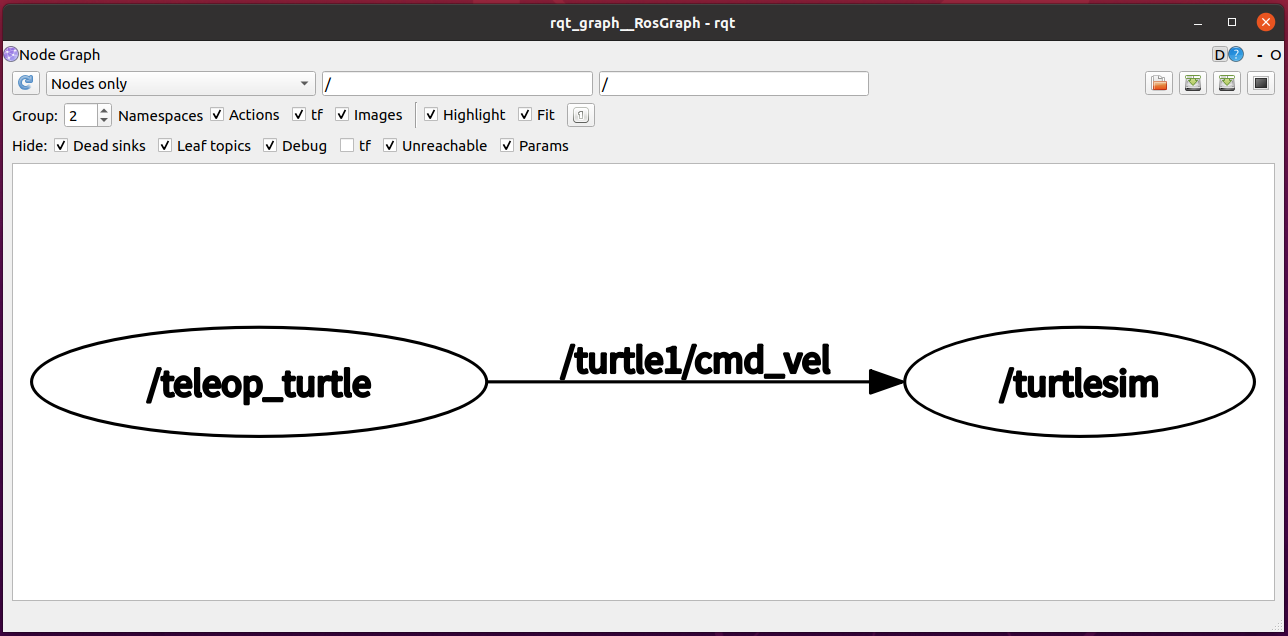
\includegraphics[width=.7\textwidth]{rqt_computing_graph.png}
  \caption{ROS计算图演示}
  \label{fig:rqt_computing_graph}
\end{figure}

\chapter{ROS通信机制}
\label{chapter:ros_communication}

机器人是一种高度复杂的系统性实现, 在机器人上可能集成各种传感器 (雷达、摄像头、GPS等等) 以及运动控制实现, 为了解耦合, 在 ROS 中每一个功能点都是一个单独的进程, 每一个进程都是独立运行的. 更确切的讲, ROS 是进程 (也称为 Nodes) 的分布式框架.  因为这些进程甚至还可分布于不同主机, 不同主机协同工作, 从而分散计算压力. 不过随之也有一个问题: 不同的进程是如何通信的? 也即不同进程间如何实现数据交换的? 在此我们就需要介绍一下 ROS 中的通信机制了.

ROS 中的基本通信机制主要有如下三种实现策略:

\begin{itemize}
  \item 话题通信 (发布订阅模式);
  \item 服务通信 (请求响应模式);
  \item 参数服务器 (参数共享模式).
\end{itemize}

本章的主要内容就是是介绍各个通信机制的应用场景、理论模型、代码实现以及相关操作命令. 本章预期达成学习目标如下:

\begin{itemize}
  \item 能够熟练介绍 ROS 中常用的通信机制;
  \item 能够理解 ROS 中每种通信机制的理论模型;
  \item 能够以代码的方式实现各种通信机制对应的案例;
  \item 能够熟练使用 ROS 中的一些操作命令;
  \item 能够独立完成相关实操案例.
\end{itemize}

\section{话题通信}

\subsection{话题通信理论模型}

话题通信实现模型是比较复杂的, 该模型如下图所示, 该模型中涉及到三个角色:

\begin{itemize}
  \item ROS Master (管理者);
  \item Talker (发布者);
  \item Listener (订阅者).
\end{itemize}

ROS Master 负责保管 Talker 和 Listener 注册的信息, 并匹配话题相同的 Talker 与 Listener, 帮助 Talker 与 Listener 建立连接, 连接建立后, Talker 可以发布消息, 且发布的消息会被 Listener 订阅.

\begin{figure}[!ht]
  \centering
  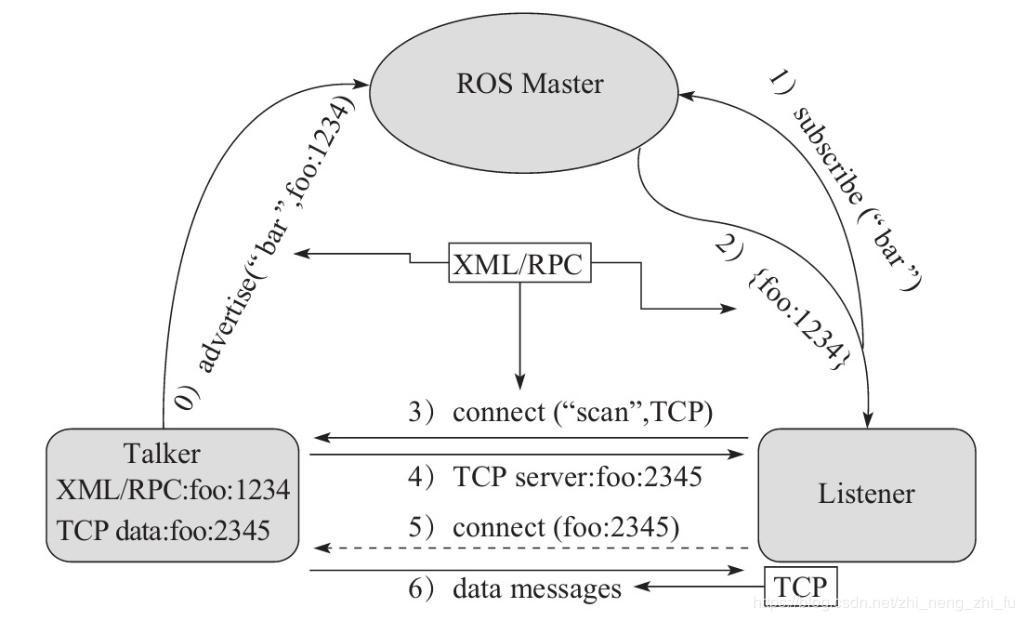
\includegraphics[width=.75\textwidth]{ros_topic_communication.jpg}
  \caption{话题通信理论模型}
  \label{fig:ros_topic_communication}
\end{figure}

整个流程由以下步骤实现:

0. Talker 注册

Talker 启动后, 会通过 RPC 在 ROS Master 中注册自身信息, 其中包含所发布消息的话题名称. ROS Master 会将节点的注册信息加入到注册表中.

1. Listener 注册

Listener 启动后, 也会通过 RPC 在 ROS Master 中注册自身信息, 包含需要订阅消息的话题名. ROS Master 会将节点的注册信息加入到注册表中.

2. ROS Master 实现信息匹配

ROS Master 会根据注册表中的信息匹配 Talker 和 Listener, 并通过 RPC 向 Listener 发送 Talker 的 RPC 地址信息.

3. Listener 向 Talker 发送请求

Listener 根据接收到的 RPC 地址, 通过 RPC 向 Talker 发送连接请求, 传输订阅的话题名称、消息类型以及通信协议 (TCP/UDP).

4. Talker 确认请求

Talker 接收到 Listener 的请求后, 也是通过 RPC 向 Listener 确认连接信息, 并发送自身的 TCP 地址信息.

5. Listener 与 Talker 件里连接

Listener 根据步骤4返回的消息使用 TCP 与 Talker 建立网络连接.

6. Talker 向 Listener 发送消息

连接建立后, Talker 开始向 Listener 发布消息.

注意:
\begin{itemize}
  \item 上述实现流程中, 前五步使用的 RPC协议, 最后两步使用的是 TCP 协议;
  \item Talker 与 Listener 的启动无先后顺序要求;
  \item Talker 与 Listener 都可以有多个;
  \item Talker 与 Listener 连接建立后, 不再需要 ROS Master. 也即, 即便关闭 ROS Master, Talker 与 Listern 照常通信.
\end{itemize}

\subsection{话题通信基本操作A (C++)}

需求: 编写发布订阅实现, 要求发布方以 10 Hz (每秒 10 次) 的频率发布文本消息, 订阅方订阅消息并将消息内容打印输出.

分析: 在模型实现中, ROS master 不需要实现, 而连接的建立也已经被封装了, 需要关注的关键点有三个:

\begin{itemize}
  \item 发布方;
  \item 接收方;
  \item 数据 (此处为普通文本).
\end{itemize}

流程:

\begin{itemize}
  \item 编写发布方实现; 
  \item 编写订阅方实现; 
  \item 编辑配置文件; 
  \item 编译并执行.
\end{itemize}

1. 发布方

\begin{cpp}
  /*
      需求: 实现基本的话题通信, 一方发布数据, 一方接收数据, 
          实现的关键点:
          1. 发送方
          2. 接收方
          3. 数据 (此处为普通文本)
          PS: 二者需要设置相同的话题

      消息发布方:
          循环发布信息:HelloWorld 后缀数字编号

      实现流程:
          1. 包含头文件 
          2. 初始化 ROS 节点:命名 (唯一)
          3. 实例化 ROS 句柄
          4. 实例化 发布者 对象
          5. 组织被发布的数据, 并编写逻辑发布数据
  */

  // 1. 包含头文件 
  #include "ros/ros.h"
  #include "std_msgs/String.h" // 普通文本类型的消息
  #include <sstream>

  int main(int argc, char  *argv[])
  {   
      // 设置编码
      setlocale(LC_ALL,"");

      // 2. 初始化 ROS 节点:命名 (唯一)
      // 参数1和参数2 后期为节点传值会使用
      // 参数3 是节点名称, 是一个标识符, 需要保证运行后, 在 ROS 网络拓扑中唯一
      ros::init(argc,argv,"talker");
      // 3. 实例化 ROS 句柄
      ros::NodeHandle nh; // 该类封装了 ROS 中的一些常用功能

      // 4. 实例化 发布者 对象
      // 泛型: 发布的消息类型
      // 参数1: 要发布到的话题
      // 参数2: 队列中最大保存的消息数, 超出此阀值时, 先进的先销毁 (时间早的先销毁)
      ros::Publisher pub = nh.advertise<std_msgs::String>("chatter",10);

      // 5. 组织被发布的数据, 并编写逻辑发布数据
      // 数据 (动态组织)
      std_msgs::String msg;
      // msg.data = "你好啊!!!";
      std::string msg_front = "Hello 你好!"; // 消息前缀
      int count = 0; // 消息计数器

      // 逻辑 (一秒10次)
      ros::Rate r(1);

      // 节点不死
      while (ros::ok())
      {
          // 使用 stringstream 拼接字符串与编号
          std::stringstream ss;
          ss << msg_front << count;
          msg.data = ss.str();
          // 发布消息
          pub.publish(msg);
          // 加入调试, 打印发送的消息
          ROS_INFO("发送的消息:%s",msg.data.c_str());

          // 根据前面制定的发送贫频率自动休眠 休眠时间 = 1/频率; 
          r.sleep();
          count++; // 循环结束前, 让 count 自增
          // 暂无应用
          ros::spinOnce();
      }


      return 0;
  }
\end{cpp}

2. 订阅方

\begin{cpp}
  /*
      需求: 实现基本的话题通信, 一方发布数据, 一方接收数据, 
          实现的关键点:
          1. 发送方
          2. 接收方
          3. 数据 (此处为普通文本)


      消息订阅方:
          订阅话题并打印接收到的消息

      实现流程:
          1. 包含头文件 
          2. 初始化 ROS 节点:命名 (唯一)
          3. 实例化 ROS 句柄
          4. 实例化 订阅者 对象
          5. 处理订阅的消息 (回调函数)
          6. 设置循环调用回调函数

  */
  // 1. 包含头文件 
  #include "ros/ros.h"
  #include "std_msgs/String.h"

  void doMsg(const std_msgs::String::ConstPtr& msg_p){
      ROS_INFO("我听见:%s",msg_p->data.c_str());
      // ROS_INFO("我听见:%s",(*msg_p).data.c_str());
  }
  int main(int argc, char  *argv[])
  {
      setlocale(LC_ALL,"");
      // 2. 初始化 ROS 节点:命名 (唯一)
      ros::init(argc,argv,"listener");
      // 3. 实例化 ROS 句柄
      ros::NodeHandle nh;

      // 4. 实例化 订阅者 对象
      ros::Subscriber sub = nh.subscribe<std_msgs::String>("chatter",10,doMsg);
      // 5. 处理订阅的消息 (回调函数)

      //     6. 设置循环调用回调函数
      ros::spin(); // 循环读取接收的数据, 并调用回调函数处理

      return 0;
  }
\end{cpp}

3. 配置 \verb|CMakeLists.txt|

\begin{bash}
  add_executable(Hello_pub
    src/Hello_pub.cpp
  )
  add_executable(Hello_sub
    src/Hello_sub.cpp
  )

  target_link_libraries(Hello_pub
    ${catkin_LIBRARIES}
  )
  target_link_libraries(Hello_sub
    ${catkin_LIBRARIES}
  )
\end{bash}

4. 执行

\begin{itemize}
  \item 启动 \verb|roscore|;
  \item 启动发布节点;
  \item 启动订阅节点.
\end{itemize}

运行结果与引言部分的演示案例1类似.

5. 注意

补充0: vscode 中的 \verb|main| 函数 声明 \verb|int main(int argc, char const *argv[]){}|, 默认生成 \verb|argv| 被 \verb|const| 修饰, 需要去除该修饰符.

补充1: \verb|ros/ros.h No such file or directory .....|

检查 \verb|CMakeList.txt| \verb|find_package| 出现重复, 删除内容少的即可

\href{https://answers.ros.org/question/237494/fatal-error-rosrosh-no-such-file-or-directory/}{参考资料}

补充2: \verb|find_package| 不添加一些包, 也可以运行啊,  ros.wiki 答案如下:

{\itshape You may notice that sometimes your project builds fine even if you did not call \verb|find_package| with all dependencies. This is because catkin combines all your projects into one, so if an earlier project calls \verb|find_package|, yours is configured with the same values. But forgetting the call means your project can easily break when built in isolation.}

补充3: 订阅时, 第一条数据丢失.

原因: 发送第一条数据时, publisher 还未在 \verb|roscore| 注册完毕.

解决: 注册后, 加入休眠 \verb|ros::Duration(3.0).sleep()|; 延迟第一条数据的发送.

PS: 可以使用 \verb|rqt_graph| 查看节点关系.

\subsection{话题通信基本操作B (Python)}

需求: 编写发布订阅实现, 要求发布方以 10 Hz (每秒 10 次)的频率发布文本消息, 订阅方订阅消息并将消息内容打印输出.

分析: 在模型实现中, ROS master 不需要实现, 而连接的建立也已经被封装了, 需要关注的关键点有三个:

\begin{itemize}
  \item 发布方
  \item 接收方
  \item 数据 (此处为普通文本)
\end{itemize}

流程:

\begin{itemize}
  \item 编写发布方实现; 
  \item 编写订阅方实现; 
  \item 为python文件添加可执行权限; 
  \item 编辑配置文件; 
  \item 编译并执行.
\end{itemize}

1. 发布方

\begin{python}
  #! /usr/bin/env python
  """
      需求: 实现基本的话题通信, 一方发布数据, 一方接收数据, 
          实现的关键点:
          1. 发送方
          2. 接收方
          3. 数据 (此处为普通文本)
          PS: 二者需要设置相同的话题

      消息发布方:
          循环发布信息: HelloWorld 后缀数字编号

      实现流程:
          1. 导包 
          2. 初始化 ROS 节点: 命名 (唯一)
          3. 实例化 发布者 对象
          4. 组织被发布的数据, 并编写逻辑发布数据
  """

  # 1. 导包 
  import rospy
  from std_msgs.msg import String

  if __name__ == "__main__":
      # 2. 初始化 ROS 节点: 命名 (唯一)
      rospy.init_node("talker_p")
      # 3. 实例化 发布者 对象
      pub = rospy.Publisher("chatter",String,queue_size=10)
      # 4. 组织被发布的数据, 并编写逻辑发布数据
      msg = String()  # 创建 msg 对象
      msg_front = "hello 你好"
      count = 0  # 计数器 
      # 设置循环频率
      rate = rospy.Rate(1)
      while not rospy.is_shutdown():

          # 拼接字符串
          msg.data = msg_front + str(count)

          pub.publish(msg)
          rate.sleep()
          rospy.loginfo("写出的数据:%s",msg.data)
          count += 1
\end{python}

2. 订阅方

\begin{python}
  #! /usr/bin/env python
  """
      需求: 实现基本的话题通信, 一方发布数据, 一方接收数据, 
          实现的关键点:
          1. 发送方
          2. 接收方
          3. 数据 (此处为普通文本)

      消息订阅方:
          订阅话题并打印接收到的消息

      实现流程:
          1. 导包 
          2. 初始化 ROS 节点: 命名 (唯一)
          3. 实例化 订阅者 对象
          4. 处理订阅的消息 (回调函数)
          5. 设置循环调用回调函数
  """

  # 1. 导包 
  import rospy
  from std_msgs.msg import String

  def doMsg(msg):
      rospy.loginfo("I heard:%s",msg.data)

  if __name__ == "__main__":
      # 2. 初始化 ROS 节点:命名 (唯一)
      rospy.init_node("listener_p")
      # 3. 实例化 订阅者 对象
      sub = rospy.Subscriber("chatter",String,doMsg,queue_size=10)
      # 4. 处理订阅的消息 (回调函数)
      # 5. 设置循环调用回调函数
      rospy.spin()
\end{python}

3. 添加可执行权限

终端下进入 \verb|scripts| 执行:

\begin{bash}
  chmod +x *.py
\end{bash}

4. 配置 \verb|CMakeLists.txt|

\begin{bash}
  catkin_install_python(PROGRAMS
    scripts/talker_p.py
    scripts/listener_p.py
    DESTINATION ${CATKIN_PACKAGE_BIN_DESTINATION}
  )
\end{bash}

5. 执行

\begin{itemize}
  \item 启动 \verb|roscore|;
  \item 启动发布节点;
  \item 启动订阅节点.
\end{itemize}

运行结果与引言部分的演示案例1类似.

PS: 可以使用 \verb|rqt_graph| 查看节点关系.

\subsection{话题通信自定义msg}

在 ROS 通信协议中, 数据载体是一个较为重要组成部分, ROS 中通过 \verb|std_msgs| 封装了一些原生的数据类型, 比如: String、Int32、Int64、Char、Bool、Empty 等等. 但是, 这些数据一般只包含一个 \verb|data| 字段, 结构的单一意味着功能上的局限性, 当传输一些复杂的数据, 比如: 激光雷达的信息. \verb|std_msgs| 由于描述性较差而显得力不从心, 这种场景下可以使用自定义的消息类型. \verb|msgs| 只是简单的文本文件, 每行具有字段类型和字段名称, 可以使用的字段类型有: 

\begin{itemize}
  \item int8, int16, int32, int64 (或者无符号类型: uint*);
  \item float32, float64;
  \item string;
  \item time, duration;
  \item other msg files;
  \item variable-length array[] and fixed-length array[C].
\end{itemize}

ROS 中还有一种特殊类型: Header, 标头包含时间戳和 ROS 中常用的坐标帧信息. 会经常看到 \verb|msg| 文件的第一行具有 Header 标头.

需求: 创建自定义消息, 该消息包含人的信息: 姓名、身高、年龄等.

流程:

\begin{itemize}
  \item 按照固定格式创建 \verb|msg| 文件;
  \item 编辑配置文件;
  \item 编译生成可以被 Python 或 C++ 调用的中间文件.
\end{itemize}

1. 定义 \verb|msg| 文件

功能包下新建 \verb|msg| 目录, 添加文件 \verb|Person.msg|.

\begin{cpp}
  string name
  uint16 age
  float64 height
\end{cpp}

2. 编辑配置文件

\verb|package.xml| 中添加编译依赖与执行依赖:

\begin{xml}
  <build_depend>message_generation</build_depend>
  <exec_depend>message_runtime</exec_depend>
  <!-- 
  exce_depend 以前对应的是 run_depend 现在非法
  -->
\end{xml}

\verb|CMakeLists.txt| 编辑 \verb|msg| 相关配置:

\begin{bash}
  find_package(catkin REQUIRED COMPONENTS
    roscpp
    rospy
    std_msgs
    message_generation
  )
  # 需要加入 message_generation, 必须有 std_msgs

  ## 配置 msg 源文件
  add_message_files(
    FILES
    Person.msg
  )

  # 生成消息时依赖于 std_msgs
  generate_messages(
    DEPENDENCIES
    std_msgs
  )

  # 执行时依赖
  catkin_package(
  #  INCLUDE_DIRS include
  #  LIBRARIES demo02_talker_listener
    CATKIN_DEPENDS roscpp rospy std_msgs message_runtime
  #  DEPENDS system_lib
  )
\end{bash}

3. 编译

编译后的中间文件查看:

C++ 需要调用的中间文件:

\begin{bash}
  .../工作空间/devel/include/包名/xxx.h
\end{bash}

\begin{figure}[!ht]
  \centering
  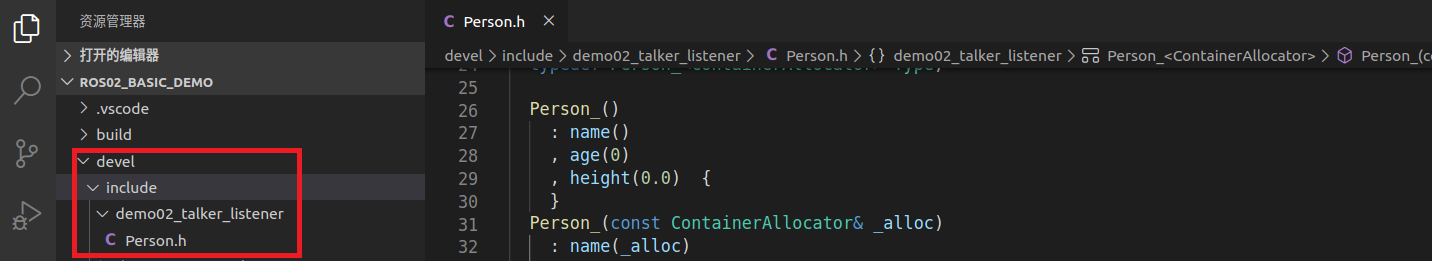
\includegraphics[width=.9\textwidth]{customized_msg_vscode_cpp.png}
  \caption{C++需要调用的中间文件}
  \label{fig:cusomized_msg_vscode_cpp}
\end{figure}

Python 需要调用的中间文件:

\begin{bash}
  .../工作空间/devel/lib/python3/dist-packages/包名/msg
\end{bash}

\begin{figure}[!ht]
  \centering
  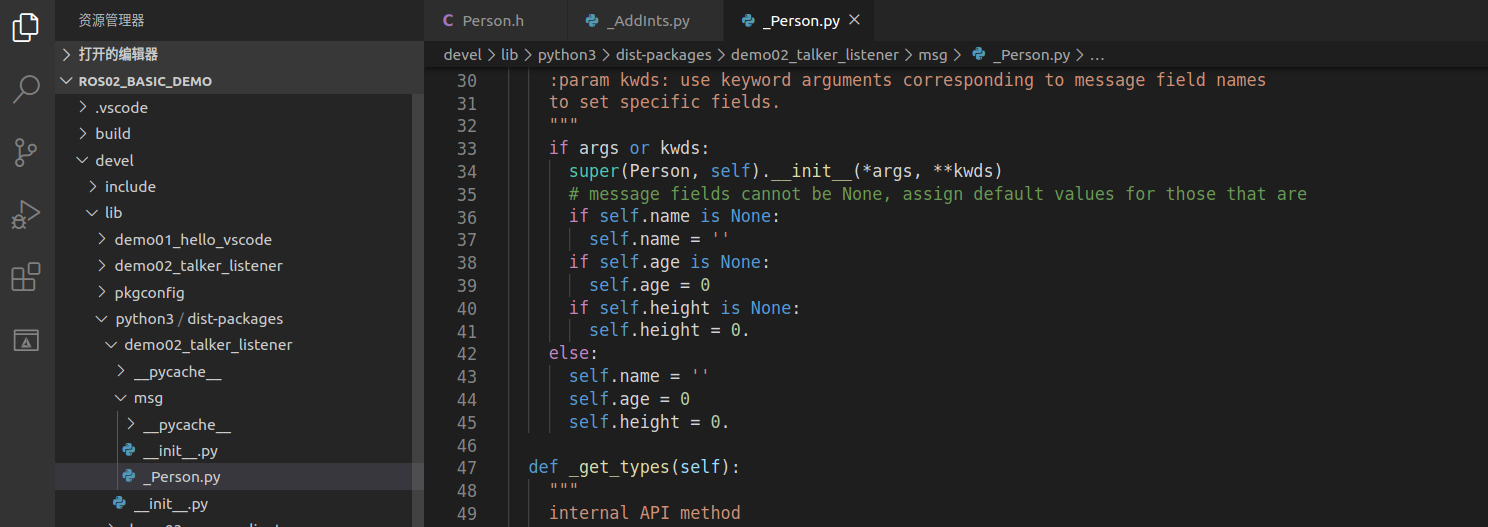
\includegraphics[width=.9\textwidth]{customized_msg_vscode_python.png}
  \caption{Python需要调用的中间文件}
  \label{fig:cusomized_msg_vscode_python}
\end{figure}

后续调用相关 \verb|msg| 时, 是从这些中间文件调用的

\subsection{话题通信自定义msg调用A (C++)}

需求: 编写发布订阅实现, 要求发布方以 10 Hz (每秒 10 次)的频率发布自定义消息, 订阅方订阅自定义消息并将消息内容打印输出.

分析: 在模型实现中, ROS master 不需要实现, 而连接的建立也已经被封装了, 需要关注的关键点有三个:

\begin{itemize}
  \item 发布方;
  \item 接收方;
  \item 数据 (此处为自定义消息).
\end{itemize}

流程:

\begin{itemize}
  \item 编写发布方实现; 
  \item 编写订阅方实现; 
  \item 编辑配置文件; 
  \item 编译并执行.
\end{itemize}

0. VSCode 配置

为了方便代码提示以及避免误抛异常, 需要先配置 VSCode, 将前面生成的 \verb|head| 文件路径配置进 \verb|c_cpp_properties.json| 的 \verb|includepath| 属性:

\begin{xml}
  {
      "configurations": [
          {
              "browse": {
                  "databaseFilename": "",
                  "limitSymbolsToIncludedHeaders": true
              },
              "includePath": [
                  "/opt/ros/noetic/include/**",
                  "/usr/include/**",
                  "/xxx/yyy工作空间/devel/include/**" // 配置 head 文件的路径 
              ],
              "name": "ROS",
              "intelliSenseMode": "gcc-x64",
              "compilerPath": "/usr/bin/gcc",
              "cStandard": "c11",
              "cppStandard": "c++17"
          }
      ],
      "version": 4
  }
\end{xml}

1. 发布方

\begin{cpp}
  /*
      需求: 循环发布人的信息
  */

  #include "ros/ros.h"
  #include "demo02_talker_listener/Person.h"

  int main(int argc, char *argv[])
  {
      setlocale(LC_ALL,"");

      // 1. 初始化 ROS 节点
      ros::init(argc,argv,"talker_person");

      // 2. 创建 ROS 句柄
      ros::NodeHandle nh;

      // 3. 创建发布者对象
      ros::Publisher pub = nh.advertise<demo02_talker_listener::Person>("chatter_person",1000);

      // 4. 组织被发布的消息, 编写发布逻辑并发布消息
      demo02_talker_listener::Person p;
      p.name = "sunwukong";
      p.age = 2000;
      p.height = 1.45;

      ros::Rate r(1);
      while (ros::ok())
      {
          pub.publish(p);
          p.age += 1;
          ROS_INFO("我叫:%s, 今年%d岁, 高%.2f米", p.name.c_str(), p.age, p.height);

          r.sleep();
          ros::spinOnce();
      }
      return 0;
  }
\end{cpp}

2. 订阅方

\begin{cpp}
  /*
      需求: 订阅人的信息
  */

  #include "ros/ros.h"
  #include "demo02_talker_listener/Person.h"

  void doPerson(const demo02_talker_listener::Person::ConstPtr& person_p){
      ROS_INFO("订阅的人信息:%s, %d, %.2f", person_p->name.c_str(), person_p->age, person_p->height);
  }

  int main(int argc, char *argv[])
  {   
      setlocale(LC_ALL,"");

      // 1. 初始化 ROS 节点
      ros::init(argc,argv,"listener_person");
      // 2. 创建 ROS 句柄
      ros::NodeHandle nh;
      // 3. 创建订阅对象
      ros::Subscriber sub = nh.subscribe<demo02_talker_listener::Person>("chatter_person",10,doPerson);

      // 4. 回调函数中处理 person

      // 5. ros::spin();
      ros::spin();    
      return 0;
  }
\end{cpp}

3. 配置 \verb|CMakeLists.txt|

需要添加 \verb|add_dependencies| 用以设置所依赖的消息相关的中间文件.

\begin{bash}
  add_executable(person_talker src/person_talker.cpp)
  add_executable(person_listener src/person_listener.cpp)

  add_dependencies(person_talker ${PROJECT_NAME}_generate_messages_cpp)
  add_dependencies(person_listener ${PROJECT_NAME}_generate_messages_cpp)

  target_link_libraries(person_talker
    ${catkin_LIBRARIES}
  )
  target_link_libraries(person_listener
    ${catkin_LIBRARIES}
  )
\end{bash}

4. 执行

\begin{itemize}
  \item 启动 \verb|roscore|;
  \item 启动发布节点;
  \item 启动订阅节点.
\end{itemize}

运行结果与引言部分的演示案例2类似.

PS: 可以使用 \verb|rqt_graph| 查看节点关系.

\subsection{话题通信自定义msg调用B (Python)}

需求: 编写发布订阅实现, 要求发布方以 1 Hz (每秒1次) 的频率发布自定义消息, 订阅方订阅自定义消息并将消息内容打印输出.

分析: 在模型实现中, ROS master 不需要实现, 而连接的建立也已经被封装了, 需要关注的关键点有三个:

\begin{itemize}
  \item 发布方;
  \item 接收方;
  \item 数据 (此处为自定义消息).
\end{itemize}

流程:

\begin{itemize}
  \item 编写发布方实现; 
  \item 编写订阅方实现; 
  \item 为 Python 文件添加可执行权限; 
  \item 编辑配置文件; 
  \item 编译并执行.
\end{itemize}

0. VSCode 配置

为了方便代码提示以及误抛异常, 需要先配置 VSCode, 将前面生成的  Python 文件路径配置进 \verb|settings.json|.

\begin{xml}
  {
      "python.autoComplete.extraPaths": [
          "/opt/ros/noetic/lib/python3/dist-packages",
          "/xxx/yyy工作空间/devel/lib/python3/dist-packages"
      ]
  }
\end{xml}

1. 发布方

\begin{python}
  #! /usr/bin/env python
  """
      发布方:
          循环发送消息
  """
  import rospy
  from demo02_talker_listener.msg import Person

  if __name__ == "__main__":
      # 1. 初始化 ROS 节点
      rospy.init_node("talker_person_p")
      # 2. 创建发布者对象
      pub = rospy.Publisher("chatter_person",Person,queue_size=10)
      # 3. 组织消息
      p = Person()
      p.name = "葫芦瓦"
      p.age = 18
      p.height = 0.75

      # 4. 编写消息发布逻辑
      rate = rospy.Rate(1)
      while not rospy.is_shutdown():
          pub.publish(p)  # 发布消息
          rate.sleep()  # 休眠
          rospy.loginfo("姓名:%s, 年龄:%d, 身高:%.2f",p.name, p.age, p.height)
\end{python}

2. 订阅方

\begin{python}
  #! /usr/bin/env python
  """
      订阅方:
          订阅消息
  """
  import rospy
  from demo02_talker_listener.msg import Person

  def doPerson(p):
      rospy.loginfo("接收到的人的信息:%s, %d, %.2f",p.name, p.age, p.height)

  if __name__ == "__main__":
      # 1. 初始化节点
      rospy.init_node("listener_person_p")
      # 2. 创建订阅者对象
      sub = rospy.Subscriber("chatter_person",Person,doPerson,queue_size=10)
      rospy.spin() # 4. 循环
\end{python}

3. 权限设置

终端下进入 \verb|scripts| 执行:

\begin{bash}
  chmod +x *.py
\end{bash}

4. 配置 \verb|CMakeLists.txt|

\begin{bash}
  catkin_install_python(PROGRAMS
    scripts/talker_p.py
    scripts/listener_p.py
    scripts/person_talker.py
    scripts/person_listener.py
    DESTINATION ${CATKIN_PACKAGE_BIN_DESTINATION}
  )
\end{bash}

5. 执行

\begin{itemize}
  \item 启动 \verb|roscore|;
  \item 启动发布节点;
  \item 启动订阅节点.
\end{itemize}

运行结果与引言部分的演示案例2类似.

PS: 可以使用 \verb|rqt_graph| 查看节点关系.

\section{服务通信}

服务通信也是 ROS 中一种极其常用的通信模式, 服务通信是基于请求响应模式的, 是一种应答机制. 也即: 一个节点 A 向另一个节点 B 发送请求, B接收处理请求并产生响应结果返回给A. 比如如下场景: 机器人巡逻过程中, 控制系统分析传感器数据发现可疑物体或人, 此时需要拍摄照片并留存.

在上述场景中, 就使用到了服务通信. 一个节点需要向相机节点发送拍照请求, 相机节点处理请求, 并返回处理结果. 与上述应用类似的, 服务通信更适用于对时时性有要求、具有一定逻辑处理的应用场景.

概念: 以请求响应的方式实现不同节点之间数据交互的通信模式.

作用: 用于偶然的、对时时性有要求、有一定逻辑处理需求的数据传输场景.

案例: 实现两个数字的求和, 客户端节点, 运行会向服务器发送两个数字, 服务器端节点接收两个数字求和并将结果响应回客户端.

\subsection{服务通信理论模型}

服务通信较之于话题通信更简单些, 理论模型如下图所示, 该模型中涉及到三个角色:

\begin{itemize}
  \item ROS master (管理者);
  \item Server (服务端);
  \item Client (客户端).
\end{itemize}

ROS Master 负责保管 Server 和 Client 注册的信息, 并匹配话题相同的 Server 与 Client, 帮助 Server 与 Client 建立连接, 连接建立后, Client 发送请求信息, Server 返回响应信息.

\begin{figure}[!ht]
  \centering
  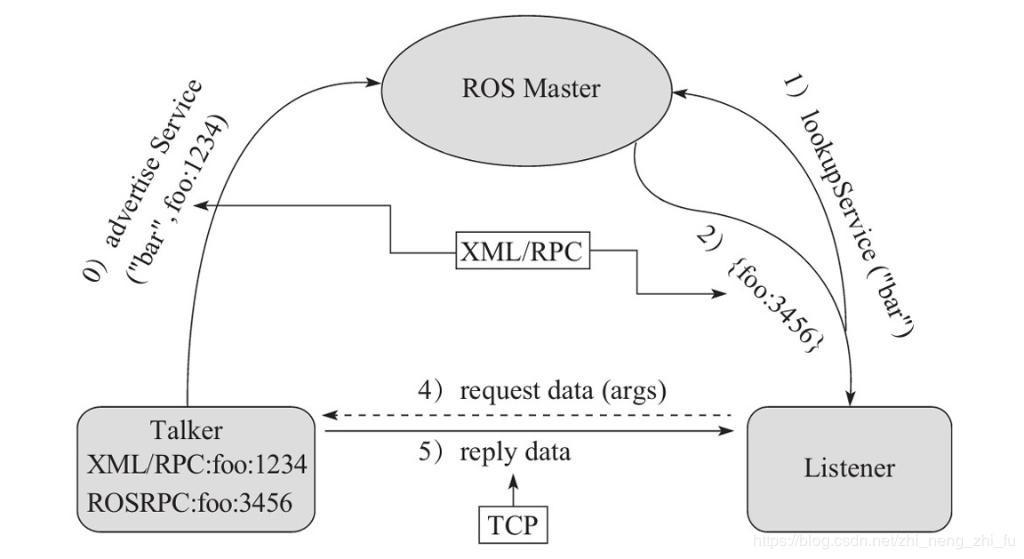
\includegraphics[width=.75\textwidth]{ros_server_communication.jpg}
  \caption{服务通信理论模型}
  \label{fig:ros_server_communication}
\end{figure}

整个流程由以下步骤实现:

0. Server注册

Server 启动后, 会通过 RPC 在 ROS Master 中注册自身信息, 其中包含提供的服务的名称. ROS Master 会将节点的注册信息加入到注册表中.

1. Client 注册

Client 启动后, 也会通过 RPC 在 ROS Master 中注册自身信息, 包含需要请求的服务的名称. ROS Master 会将节点的注册信息加入到注册表中.

2. ROS Master 实现信息匹配

ROS Master 会根据注册表中的信息匹配 Server 和 Client, 并通过 RPC 向 Client 发送 Server 的 TCP 地址信息.

3. Client 发送请求

Client 根据步骤2响应的信息, 使用 TCP 与 Server 建立网络连接, 并发送请求数据.

4. Server 发送响应

Server 接收、解析请求的数据, 并产生响应结果返回给 Client.

注意:

\begin{itemize}
  \item 客户端请求被处理时, 需要保证服务器已经启动; 
  \item 服务端和客户端都可以存在多个.
\end{itemize}

\subsection{服务通信自定义srv}

需求: 服务通信中, 客户端提交两个整数至服务端, 服务端求和并响应结果到客户端, 请创建服务器与客户端通信的数据载体.

流程: \verb|srv| 文件内的可用数据类型与 \verb|msg| 文件一致, 且定义 \verb|srv| 实现流程与自定义 \verb|msg| 实现流程类似:

\begin{itemize}
  \item 按照固定格式创建 \verb|srv| 文件;
  \item 编辑配置文件;
  \item 编译生成中间文件.
\end{itemize}

1. 定义srv文件

服务通信中, 数据分成两部分, 请求与响应, 在 srv 文件中请求和响应使用 \verb|---| 分割, 具体实现如下:

功能包下新建 \verb|srv| 目录, 添加 \verb|xxx.srv| 文件, 内容:

\begin{bash}
  # 客户端请求时发送的两个数字
  int32 num1
  int32 num2
  ---
  # 服务器响应发送的数据
  int32 sum
\end{bash}

2. 编辑配置文件

\verb|package.xml| 中添加编译依赖与执行依赖.

\begin{xml}
  <build_depend>message_generation</build_depend>
  <exec_depend>message_runtime</exec_depend>
  <!-- exce_depend 以前对应的是 run_depend 现在非法 -->
\end{xml}

\verb|CMakeLists.txt| 编辑 srv 相关配置

\begin{bash}
  find_package(catkin REQUIRED COMPONENTS
    roscpp
    rospy
    std_msgs
    message_generation
  )
  # 需要加入 message_generation, 必须有 std_msgs

  add_service_files(
    FILES
    AddInts.srv
  )

  generate_messages(
    DEPENDENCIES
    std_msgs
  )
\end{bash}

注意: 官网没有在 \verb|catkin_package| 中配置 \verb|message_runtime|, 经测试配置也可以.

3. 编译

编译后的中间文件查看:

C++ 需要调用的中间文件:

\begin{bash}
  .../工作空间/devel/include/包名/xxx.h
\end{bash}

\begin{figure}[!ht]
  \centering
  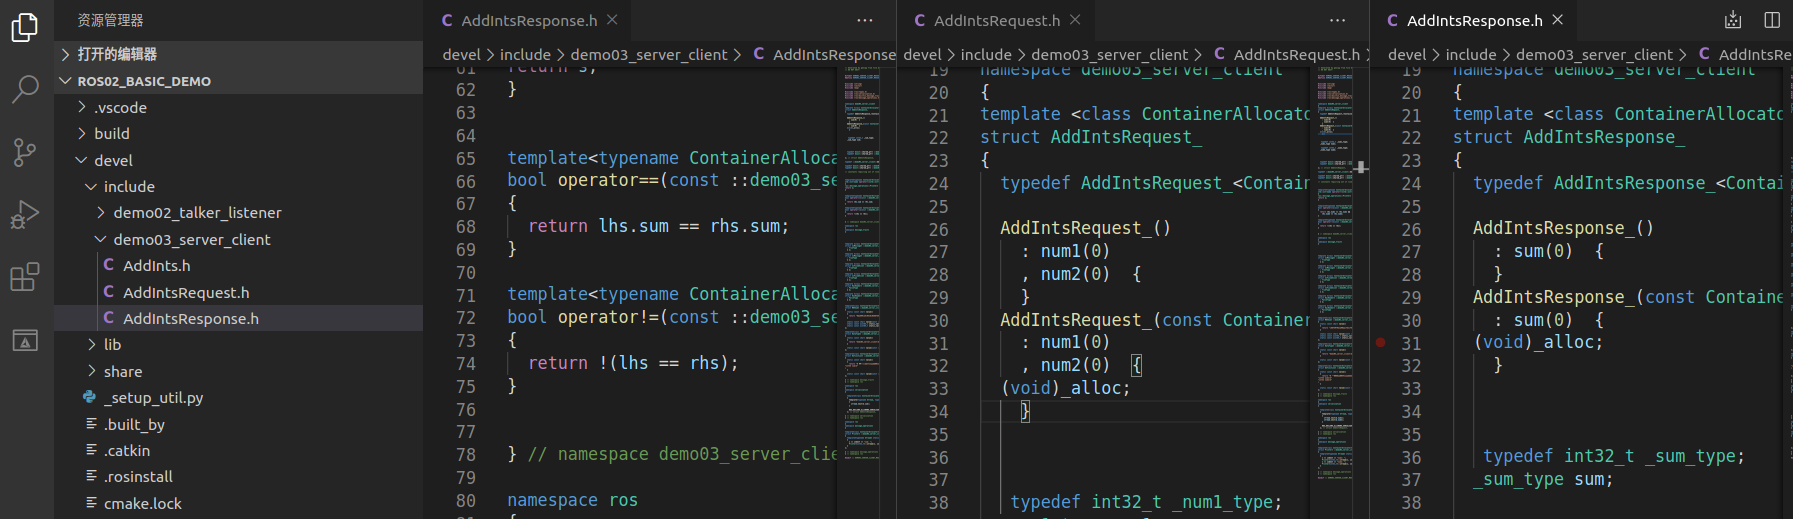
\includegraphics[width=.9\textwidth]{customized_srv_vscode_cpp.png}
  \caption{C++需要调用的中间文件}
  \label{fig:cusomized_srv_vscode_cpp}
\end{figure}

Python 需要调用的中间文件:

\begin{bash}
  .../工作空间/devel/lib/python3/dist-packages/包名/srv
\end{bash}

\begin{figure}[!ht]
  \centering
  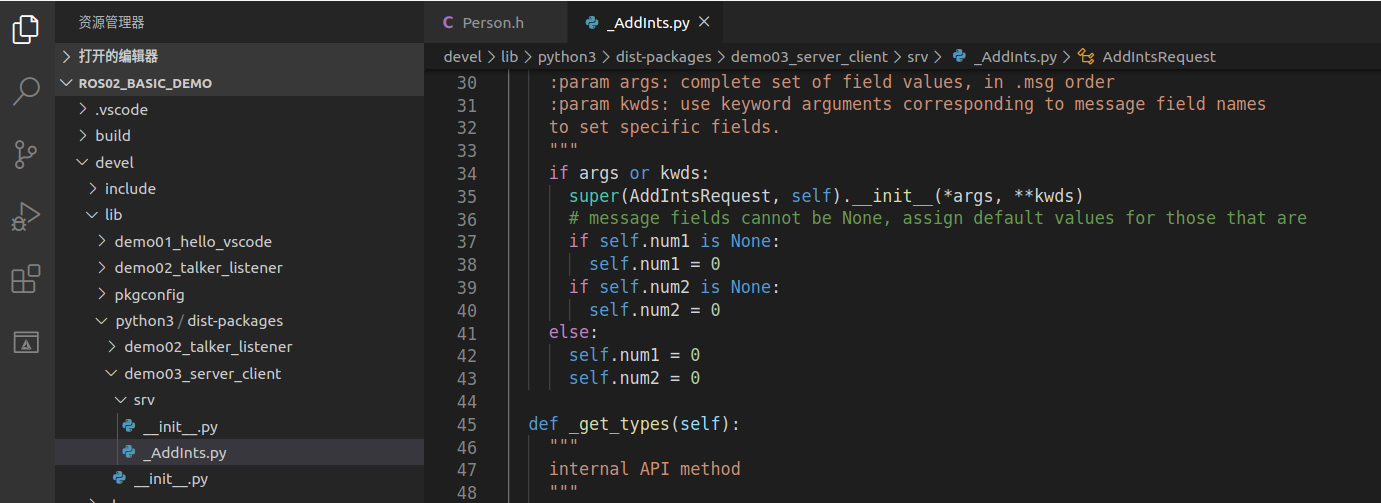
\includegraphics[width=.9\textwidth]{customized_srv_vscode_python.png}
  \caption{Python需要调用的中间文件}
  \label{fig:cusomized_srv_vscode_python}
\end{figure}

后续调用相关 srv 时, 是从这些中间文件调用的.

\subsection{服务通信自定义srv调用A (C++)}

需求: 编写服务通信, 客户端提交两个整数至服务端, 服务端求和并响应结果到客户端.

分析: 在模型实现中, ROS master 不需要实现, 而连接的建立也已经被封装了, 需要关注的关键点有三个:

\begin{itemize}
  \item 服务端
  \item 客户端
  \item 数据
\end{itemize}

流程:

\begin{itemize}
  \item 编写服务端实现; 
  \item 编写客户端实现; 
  \item 编辑配置文件; 
  \item 编译并执行.
\end{itemize}

0. VSCode 配置

需要像之前自定义 \verb|msg| 实现一样配置 \verb|c_cpp_properies.json| 文件, 如果以前已经配置且没有变更工作空间, 可以忽略, 如果需要配置, 配置方式与之前相同:

\begin{xml}
  {
      "configurations": [
          {
              "browse": {
                  "databaseFilename": "",
                  "limitSymbolsToIncludedHeaders": true
              },
              "includePath": [
                  "/opt/ros/noetic/include/**",
                  "/usr/include/**",
                  "/xxx/yyy工作空间/devel/include/**" // 配置 head 文件的路径 
              ],
              "name": "ROS",
              "intelliSenseMode": "gcc-x64",
              "compilerPath": "/usr/bin/gcc",
              "cStandard": "c11",
              "cppStandard": "c++17"
          }
      ],
      "version": 4
  }
\end{xml}

1. 服务端

\begin{cpp}
  /*
      需求: 
          编写两个节点实现服务通信, 客户端节点需要提交两个整数到服务器
          服务器需要解析客户端提交的数据, 相加后, 将结果响应回客户端, 
          客户端再解析

      服务器实现:
          1. 包含头文件
          2. 初始化 ROS 节点
          3. 创建 ROS 句柄
          4. 创建 服务 对象
          5. 回调函数处理请求并产生响应
          6. 由于请求有多个, 需要调用 ros::spin()
  */

  #include "ros/ros.h"
  #include "demo03_server_client/AddInts.h"

  // bool 返回值由于标志是否处理成功
  bool doReq(demo03_server_client::AddInts::Request& req,
            demo03_server_client::AddInts::Response& resp){
      int num1 = req.num1;
      int num2 = req.num2;

      ROS_INFO("服务器接收到的请求数据为:num1 = %d, num2 = %d",num1, num2);

      // 逻辑处理
      if (num1 < 0 || num2 < 0)
      {
          ROS_ERROR("提交的数据异常:数据不可以为负数");
          return false;
      }

      // 如果没有异常, 那么相加并将结果赋值给 resp
      resp.sum = num1 + num2;
      return true;
  }

  int main(int argc, char *argv[])
  {
      setlocale(LC_ALL,"");
      // 2. 初始化 ROS 节点
      ros::init(argc,argv,"AddInts_Server");
      // 3. 创建 ROS 句柄
      ros::NodeHandle nh;
      // 4. 创建 服务 对象
      ros::ServiceServer server = nh.advertiseService("AddInts",doReq);
      ROS_INFO("服务已经启动....");
      //     5. 回调函数处理请求并产生响应
      //     6. 由于请求有多个, 需要调用 ros::spin()
      ros::spin();
      return 0;
  }
\end{cpp}

2. 客户端

\begin{cpp}
  /*
      需求: 
          编写两个节点实现服务通信, 客户端节点需要提交两个整数到服务器
          服务器需要解析客户端提交的数据, 相加后, 将结果响应回客户端, 
          客户端再解析

      服务器实现:
          1. 包含头文件
          2. 初始化 ROS 节点
          3. 创建 ROS 句柄
          4. 创建 客户端 对象
          5. 请求服务, 接收响应
  */

  // 1. 包含头文件
  #include "ros/ros.h"
  #include "demo03_server_client/AddInts.h"

  int main(int argc, char *argv[])
  {
      setlocale(LC_ALL,"");

      // 调用时动态传值, 如果通过 launch 的 args 传参, 需要传递的参数个数 +3
      if (argc != 3)
      // if (argc != 5)//launch 传参 (0-文件路径 1传入的参数 2传入的参数 3节点名称 4日志路径)
      {
          ROS_ERROR("请提交两个整数");
          return 1;
      }


      // 2. 初始化 ROS 节点
      ros::init(argc,argv,"AddInts_Client");
      // 3. 创建 ROS 句柄
      ros::NodeHandle nh;
      // 4. 创建 客户端 对象
      ros::ServiceClient client = nh.serviceClient<demo03_server_client::AddInts>("AddInts");
      // 等待服务启动成功
      // 方式1
      ros::service::waitForService("AddInts");
      // 方式2
      // client.waitForExistence();
      // 5. 组织请求数据
      demo03_server_client::AddInts ai;
      ai.request.num1 = atoi(argv[1]);
      ai.request.num2 = atoi(argv[2]);
      // 6. 发送请求, 返回 bool 值, 标记是否成功
      bool flag = client.call(ai);
      // 7. 处理响应
      if (flag)
      {
          ROS_INFO("请求正常处理, 响应结果:%d",ai.response.sum);
      }
      else
      {
          ROS_ERROR("请求处理失败....");
          return 1;
      }

      return 0;
  }
\end{cpp}


3. 配置 \verb|CMakeLists.txt|

\begin{bash}
  add_executable(AddInts_Server src/AddInts_Server.cpp)
  add_executable(AddInts_Client src/AddInts_Client.cpp)

  add_dependencies(AddInts_Server ${PROJECT_NAME}_gencpp)
  add_dependencies(AddInts_Client ${PROJECT_NAME}_gencpp)

  target_link_libraries(AddInts_Server
    ${catkin_LIBRARIES}
  )
  target_link_libraries(AddInts_Client
    ${catkin_LIBRARIES}
  )
\end{bash}

4. 执行

流程:

\begin{itemize}
  \item 先启动服务: \verb|rosrun 包名 服务|
  \item 然后再调用客户端: \verb|rosrun 包名 客户端 参数1 参数2|
\end{itemize}

结果: 会根据提交的数据响应相加后的结果.

注意: 如果先启动客户端, 那么会导致运行失败

优化: 在客户端发送请求前添加: \verb|client.waitForExistence();|

或: \verb|ros::service::waitForService("AddInts");|

这是一个阻塞式函数, 只有服务启动成功后才会继续执行. 此处可以使用 launch 文件优化, 但是需要注意 \verb|args| 传参特点.

\subsection{服务通信自定义srv调用B (Python)}

需求: 编写服务通信, 客户端提交两个整数至服务端, 服务端求和并响应结果到客户端.

分析: 在模型实现中, ROS master 不需要实现, 而连接的建立也已经被封装了, 需要关注的关键点有三个:

\begin{itemize}
  \item 服务端
  \item 客户端
  \item 数据
\end{itemize}

流程:

\begin{itemize}
  \item 编写服务端实现; 
  \item 编写客户端实现; 
  \item 为 Python 文件添加可执行权限; 
  \item 编辑配置文件; 
  \item 编译并执行.
\end{itemize}

0. VSCode配置

需要像之前自定义 \verb|msg| 实现一样配置 \verb|settings.json| 文件, 如果以前已经配置且没有变更工作空间, 可以忽略, 如果需要配置, 配置方式与之前相同:

\begin{xml}
  {
      "python.autoComplete.extraPaths": [
          "/opt/ros/noetic/lib/python3/dist-packages",
      ]
  }
\end{xml}

1. 服务端

\begin{python}
  #! /usr/bin/env python
  """
      需求: 
          编写两个节点实现服务通信, 客户端节点需要提交两个整数到服务器
          服务器需要解析客户端提交的数据, 相加后, 将结果响应回客户端, 
          客户端再解析

      服务器端实现:
          1. 导包
          2. 初始化 ROS 节点
          3. 创建服务对象
          4. 回调函数处理请求并产生响应
          5. spin 函数
  """

  # 1. 导包
  import rospy
  from demo03_server_client.srv import AddInts,AddIntsRequest,AddIntsResponse
  # 回调函数的参数是请求对象, 返回值是响应对象
  def doReq(req):
      # 解析提交的数据
      sum = req.num1 + req.num2
      rospy.loginfo("提交的数据:num1 = %d, num2 = %d, sum = %d",req.num1, req.num2, sum)

      # 创建响应对象, 赋值并返回
      # resp = AddIntsResponse()
      # resp.sum = sum
      resp = AddIntsResponse(sum)
      return resp


  if __name__ == "__main__":
      # 2. 初始化 ROS 节点
      rospy.init_node("addints_server_p")
      # 3. 创建服务对象
      server = rospy.Service("AddInts",AddInts,doReq)
      # 4. 回调函数处理请求并产生响应
      # 5. spin 函数
      rospy.spin()
\end{python}

2. 客户端

\begin{python}
  #! /usr/bin/env python

  """
      需求: 
          编写两个节点实现服务通信, 客户端节点需要提交两个整数到服务器
          服务器需要解析客户端提交的数据, 相加后, 将结果响应回客户端, 
          客户端再解析

      客户端实现:
          1. 导包
          2. 初始化 ROS 节点
          3. 创建请求对象
          4. 发送请求
          5. 接收并处理响应

      优化:
          加入数据的动态获取
  """

  # 1. 导包
  import rospy
  from demo03_server_client.srv import *
  import sys

  if __name__ == "__main__":

      # 优化实现
      if len(sys.argv) != 3:
          rospy.logerr("请正确提交参数")
          sys.exit(1)


      # 2. 初始化 ROS 节点
      rospy.init_node("AddInts_Client_p")
      # 3. 创建请求对象
      client = rospy.ServiceProxy("AddInts",AddInts)
      # 请求前, 等待服务已经就绪
      # 方式1:
      # rospy.wait_for_service("AddInts")
      # 方式2
      client.wait_for_service()
      # 4. 发送请求, 接收并处理响应
      # 方式1
      # resp = client(3,4)
      # 方式2
      # resp = client(AddIntsRequest(1,5))
      # 方式3
      req = AddIntsRequest()
      # req.num1 = 100
      # req.num2 = 200 

      # 优化
      req.num1 = int(sys.argv[1])
      req.num2 = int(sys.argv[2]) 

      resp = client.call(req)
      rospy.loginfo("响应结果:%d",resp.sum)
\end{python}

3. 设置权限

终端下进入 \verb|scripts| 执行:

\begin{bash}
  chmod +x *.py
\end{bash}

4. 配置 \verb|CMakeLists.txt|

\begin{bash}
  catkin_install_python(PROGRAMS
    scripts/AddInts_Server_p.py 
    scripts/AddInts_Client_p.py
    DESTINATION ${CATKIN_PACKAGE_BIN_DESTINATION}
  )
\end{bash}

5. 执行

流程:

\begin{itemize}
  \item 先启动服务: \verb|rosrun 包名 服务|
  \item 再调用客户端: \verb|rosrun 包名 客户端 参数1 参数2|
\end{itemize}

结果: 会根据提交的数据响应相加后的结果.

\section{参数服务器}

参数服务器在 ROS 中主要用于实现不同节点之间的数据共享. 参数服务器相当于是独立于所有节点的一个公共容器, 可以将数据存储在该容器中, 被不同的节点调用, 当然不同的节点也可以往其中存储数据, 关于参数服务器的典型应用场景如下: 导航实现时, 会进行路径规划, 比如: 全局路径规划, 设计一个从出发点到目标点的大致路径. 本地路径规划, 会根据当前路况生成时时的行进路径

上述场景中, 全局路径规划和本地路径规划时, 就会使用到参数服务器: 路径规划时, 需要参考小车的尺寸, 我们可以将这些尺寸信息存储到参数服务器, 全局路径规划节点与本地路径规划节点都可以从参数服务器中调用这些参数. 参数服务器, 一般适用于存在数据共享的一些应用场景.

概念: 以共享的方式实现不同节点之间数据交互的通信模式.

作用: 存储一些多节点共享的数据, 类似于全局变量.

案例: 实现参数增删改查操作.

另请参考:

\begin{itemize}
  \item \href{http://wiki.ros.org/Parameter%20Server}{ROS/Parameter Server};
  \item \href{http://wiki.ros.org/roscpp/Overview/Parameter%20Server}{roscpp/Overview/Parameter Server};
  \item \href{http://wiki.ros.org/rospy/Overview/Parameter%20Server}{rospy/Overview/Parameter Server}.
\end{itemize}

\subsection{参数服务器理论模型}

参数服务器实现是最为简单的, 该模型如下图所示, 该模型中涉及到三个角色:

\begin{itemize}
  \item ROS Master (管理者)
  \item Talker (参数设置者)
  \item Listener (参数调用者)
\end{itemize}

ROS Master 作为一个公共容器保存参数, Talker 可以向容器中设置参数, Listener 可以获取参数.

\begin{figure}[!ht]
  \centering
  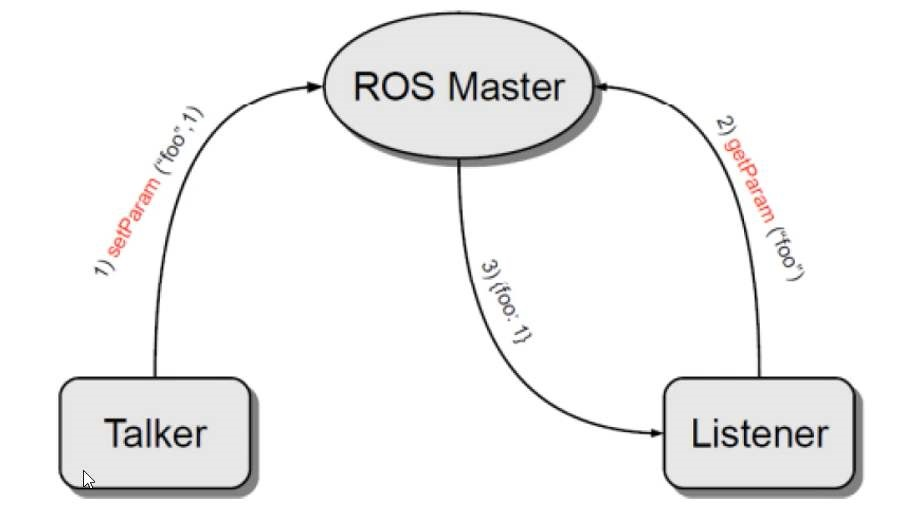
\includegraphics[width=.75\textwidth]{ros_param_server.jpg}
  \caption{参数服务器理论模型}
  \label{fig:ros_param_server}
\end{figure}

整个流程由以下步骤实现:

1. Talker 设置参数

Talker 通过 RPC 向参数服务器发送参数 (包括参数名与参数值), ROS Master 将参数保存到参数列表中.

2. Listener 获取参数

Listener 通过 RPC 向参数服务器发送参数查找请求, 请求中包含要查找的参数名.

3. ROS Master 向 Listener 发送参数值

ROS Master 根据步骤2请求提供的参数名查找参数值, 并将查询结果通过 RPC 发送给 Listener.

参数可使用数据类型:

\begin{itemize}
  \item 32-bit integers
  \item booleans
  \item strings
  \item doubles
  \item iso8601 dates
  \item lists
  \item base64-encoded binary data
  \item 字典
\end{itemize}

注意: 参数服务器不是为高性能而设计的, 因此最好用于存储静态的非二进制的简单数据.

\subsection{参数操作A (C++)}

需求: 实现参数服务器参数的增删改查操作.

在 C++ 中实现参数服务器数据的增删改查, 可以通过两套 API 实现:

\begin{itemize}
  \item \verb|ros::NodeHandle|
  \item \verb|ros::param|
\end{itemize}

下面为具体操作演示

1. 参数服务器新增 (修改)参数

\begin{cpp}
  /*
      参数服务器操作之新增与修改 (二者API一样): C++实现
      在 roscpp 中提供了两套 API 实现参数操作
      ros::NodeHandle
          setParam("键", 值)
      ros::param
          set("键","值")

      示例:分别设置整形、浮点、字符串、bool、列表、字典等类型参数
          修改 (相同的键, 不同的值)
  */

  #include "ros/ros.h"

  int main(int argc, char *argv[])
  {
      ros::init(argc,argv,"set_update_param");

      std::vector<std::string> stus;
      stus.push_back("zhangsan");
      stus.push_back("李四");
      stus.push_back("王五");
      stus.push_back("孙大脑袋");

      std::map<std::string,std::string> friends;
      friends["guo"] = "huang";
      friends["yuang"] = "xiao";

      //NodeHandle--------------------------------------------------------
      ros::NodeHandle nh;
      nh.setParam("nh_int",10); // 整型
      nh.setParam("nh_double",3.14); // 浮点型
      nh.setParam("nh_bool",true); // bool
      nh.setParam("nh_string","hello NodeHandle"); // 字符串
      nh.setParam("nh_vector",stus); // vector
      nh.setParam("nh_map",friends); // map

      // 修改演示 (相同的键, 不同的值)
      nh.setParam("nh_int",10000);

      //param--------------------------------------------------------
      ros::param::set("param_int",20);
      ros::param::set("param_double",3.14);
      ros::param::set("param_string","Hello Param");
      ros::param::set("param_bool",false);
      ros::param::set("param_vector",stus);
      ros::param::set("param_map",friends);

      // 修改演示 (相同的键, 不同的值)
      ros::param::set("param_int",20000);

      return 0;
  }
\end{cpp}

2. 参数服务器获取参数

\begin{cpp}
  /*
      参数服务器操作之查询: C++实现
      在 roscpp 中提供了两套 API 实现参数操作
      ros::NodeHandle

          param(键, 默认值) 
              存在, 返回对应结果, 否则返回默认值

          getParam(键, 存储结果的变量)
              存在, 返回 true, 且将值赋值给参数2
              若果键不存在, 那么返回值为 false, 且不为参数2赋值

          getParamCached(键, 存储结果的变量)--提高变量获取效率
              存在, 返回 true, 且将值赋值给参数2
              若果键不存在, 那么返回值为 false, 且不为参数2赋值

          getParamNames(std::vector<std::string>)
              获取所有的键, 并存储在参数 vector 中 

          hasParam(键)
              是否包含某个键, 存在返回 true, 否则返回 false

          searchParam(参数1, 参数2)
              搜索键, 参数1是被搜索的键, 参数2存储搜索结果的变量

      ros::param ----- 与 NodeHandle 类似
  */

  #include "ros/ros.h"

  int main(int argc, char *argv[])
  {
      setlocale(LC_ALL,"");
      ros::init(argc,argv,"get_param");

      //NodeHandle--------------------------------------------------------
      /*
      ros::NodeHandle nh;
      // param 函数
      int res1 = nh.param("nh_int",100); // 键存在
      int res2 = nh.param("nh_int2",100); // 键不存在
      ROS_INFO("param获取结果:%d,%d",res1,res2);

      // getParam 函数
      int nh_int_value;
      double nh_double_value;
      bool nh_bool_value;
      std::string nh_string_value;
      std::vector<std::string> stus;
      std::map<std::string, std::string> friends;

      nh.getParam("nh_int",nh_int_value);
      nh.getParam("nh_double",nh_double_value);
      nh.getParam("nh_bool",nh_bool_value);
      nh.getParam("nh_string",nh_string_value);
      nh.getParam("nh_vector",stus);
      nh.getParam("nh_map",friends);

      ROS_INFO("getParam获取的结果:%d,%.2f,%s,%d",
              nh_int_value,
              nh_double_value,
              nh_string_value.c_str(),
              nh_bool_value
              );
      for (auto &&stu : stus)
      {
          ROS_INFO("stus 元素:%s",stu.c_str());        
      }

      for (auto &&f : friends)
      {
          ROS_INFO("map 元素:%s = %s",f.first.c_str(), f.second.c_str());
      }

      // getParamCached()
      nh.getParamCached("nh_int",nh_int_value);
      ROS_INFO("通过缓存获取数据:%d",nh_int_value);

      //getParamNames()
      std::vector<std::string> param_names1;
      nh.getParamNames(param_names1);
      for (auto &&name : param_names1)
      {
          ROS_INFO("名称解析name = %s",name.c_str());        
      }
      ROS_INFO("----------------------------");

      ROS_INFO("存在 nh_int 吗? %d",nh.hasParam("nh_int"));
      ROS_INFO("存在 nh_intttt 吗? %d",nh.hasParam("nh_intttt"));

      std::string key;
      nh.searchParam("nh_int",key);
      ROS_INFO("搜索键:%s",key.c_str());
      */
      //param--------------------------------------------------------
      ROS_INFO("++++++++++++++++++++++++++++++++++++++++");
      int res3 = ros::param::param("param_int",20); // 存在
      int res4 = ros::param::param("param_int2",20); //  不存在返回默认
      ROS_INFO("param获取结果:%d,%d",res3,res4);

      // getParam 函数
      int param_int_value;
      double param_double_value;
      bool param_bool_value;
      std::string param_string_value;
      std::vector<std::string> param_stus;
      std::map<std::string, std::string> param_friends;

      ros::param::get("param_int",param_int_value);
      ros::param::get("param_double",param_double_value);
      ros::param::get("param_bool",param_bool_value);
      ros::param::get("param_string",param_string_value);
      ros::param::get("param_vector",param_stus);
      ros::param::get("param_map",param_friends);

      ROS_INFO("getParam获取的结果:%d,%.2f,%s,%d",
              param_int_value,
              param_double_value,
              param_string_value.c_str(),
              param_bool_value
              );
      for (auto &&stu : param_stus)
      {
          ROS_INFO("stus 元素:%s",stu.c_str());        
      }

      for (auto &&f : param_friends)
      {
          ROS_INFO("map 元素:%s = %s",f.first.c_str(), f.second.c_str());
      }

      // getParamCached()
      ros::param::getCached("param_int",param_int_value);
      ROS_INFO("通过缓存获取数据:%d",param_int_value);

      // getParamNames()
      std::vector<std::string> param_names2;
      ros::param::getParamNames(param_names2);
      for (auto &&name : param_names2)
      {
          ROS_INFO("名称解析name = %s",name.c_str());        
      }
      ROS_INFO("----------------------------");

      ROS_INFO("存在 param_int 吗? %d",ros::param::has("param_int"));
      ROS_INFO("存在 param_intttt 吗? %d",ros::param::has("param_intttt"));

      std::string key;
      ros::param::search("param_int",key);
      ROS_INFO("搜索键:%s",key.c_str());

      return 0;
  }
\end{cpp}

3. 参数服务器删除参数

\begin{cpp}
  /* 
      参数服务器操作之删除_C++实现:

      ros::NodeHandle
          deleteParam("键")
          根据键删除参数, 删除成功, 返回 true, 否则 (参数不存在), 返回 false

      ros::param
          del("键")
          根据键删除参数, 删除成功, 返回 true, 否则 (参数不存在), 返回 false
  */
  #include "ros/ros.h"

  int main(int argc, char *argv[])
  {   
      setlocale(LC_ALL,"");
      ros::init(argc,argv,"delete_param");

      ros::NodeHandle nh;
      bool r1 = nh.deleteParam("nh_int");
      ROS_INFO("nh 删除结果:%d",r1);

      bool r2 = ros::param::del("param_int");
      ROS_INFO("param 删除结果:%d",r2);

      return 0;
  }
\end{cpp}

\subsection{参数操作B (Python)}

需求: 实现参数服务器参数的增删改查操作.

1. 参数服务器新增 (修改)参数

\begin{python}
  #! /usr/bin/env python
  """
      参数服务器操作之新增与修改 (二者 API 一样): Python实现
  """

  import rospy

  if __name__ == "__main__":
      rospy.init_node("set_update_paramter_p")

      # 设置各种类型参数
      rospy.set_param("p_int",10)
      rospy.set_param("p_double",3.14)
      rospy.set_param("p_bool",True)
      rospy.set_param("p_string","hello python")
      rospy.set_param("p_list",["hello","haha","xixi"])
      rospy.set_param("p_dict",{"name":"hulu","age":8})

      # 修改
      rospy.set_param("p_int",100)
\end{python}

2. 参数服务器获取参数

\begin{python}
  #! /usr/bin/env python

  """
      参数服务器操作之查询: Python实现
          get_param(键, 默认值)
              当键存在时, 返回对应的值, 如果不存在返回默认值
          get_param_cached
          get_param_names
          has_param
          search_param
  """

  import rospy

  if __name__ == "__main__":
      rospy.init_node("get_param_p")

      # 获取参数
      int_value = rospy.get_param("p_int",10000)
      double_value = rospy.get_param("p_double")
      bool_value = rospy.get_param("p_bool")
      string_value = rospy.get_param("p_string")
      p_list = rospy.get_param("p_list")
      p_dict = rospy.get_param("p_dict")

      rospy.loginfo("获取的数据:%d,%.2f,%d,%s",
                  int_value,
                  double_value,
                  bool_value,
                  string_value)
      for ele in p_list:
          rospy.loginfo("ele = %s", ele)

      rospy.loginfo("name = %s, age = %d",p_dict["name"],p_dict["age"])

      # get_param_cached
      int_cached = rospy.get_param_cached("p_int")
      rospy.loginfo("缓存数据:%d",int_cached)

      # get_param_names
      names = rospy.get_param_names()
      for name in names:
          rospy.loginfo("name = %s",name)

      rospy.loginfo("-"*80)

      # has_param
      flag = rospy.has_param("p_int")
      rospy.loginfo("包含p_int吗? %d",flag)

      # search_param
      key = rospy.search_param("p_int")
      rospy.loginfo("搜索的键 = %s",key)
\end{python}

3. 参数服务器删除参数

\begin{python}
  #! /usr/bin/env python
  """
      参数服务器操作之删除: Python 实现
      rospy.delete_param("键")
      键存在时, 可以删除成功, 键不存在时, 会抛出异常
  """

  import rospy

  if __name__ == "__main__":
      rospy.init_node("delete_param_p")

      try:
          rospy.delete_param("p_int")
      except Exception as e:
          rospy.loginfo("删除失败")
\end{python}

\section{常用命令}

机器人系统中启动的节点少则几个, 多则十几个、几十个, 不同的节点名称各异, 通信时使用话题、服务、消息、参数等等都各不相同, 一个显而易见的问题是: 当需要自定义节点和其他某个已经存在的节点通信时, 如何获取对方的话题、以及消息载体的格式呢? 

在 ROS 同提供了一些实用的命令行工具, 可以用于获取不同节点的各类信息, 常用的命令如下:

\begin{itemize}
  \item \verb|rosnode|: 操作节点;
  \item \verb|rostopic|: 操作话题;
  \item \verb|rosservice|: 操作服务;
  \item \verb|rosmsg|: 操作 msg 消息;
  \item \verb|rossrv|: 操作 srv 消息;
  \item \verb|rosparam|: 操作参数.
\end{itemize}

作用: 和之前介绍的文件系统操作命令比较, 文件操作命令是静态的, 操作的是磁盘上的文件, 而上述命令是动态的, 在 ROS 程序启动后, 可以动态的获取运行中的节点或参数的相关信息.

案例: 本节将借助于 2.1、2.2 和 2.3 的通信实现介绍相关命令的基本使用, 并通过练习 ROS 内置的小海龟例程来强化命令的应用.

另请参考: \href{http://wiki.ros.org/ROS/CommandLineTools}{ROS/CommandLineTools}.

\begin{figure}[!ht]
  \centering
  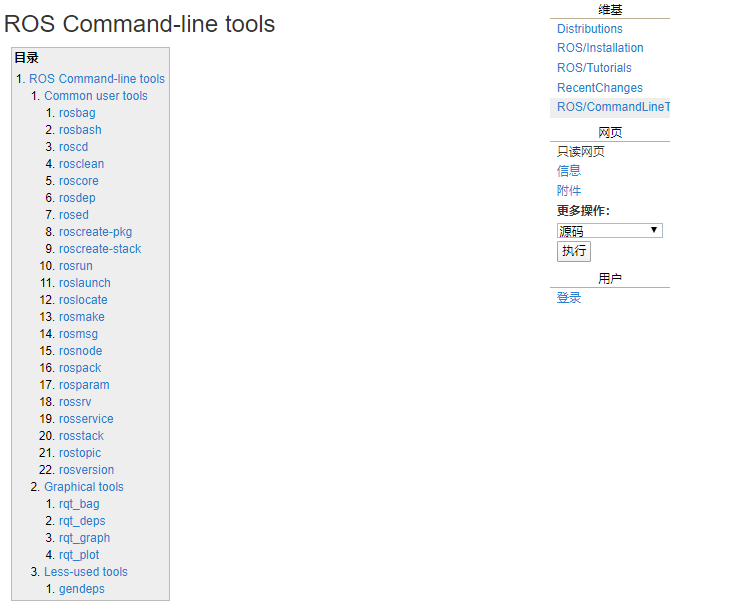
\includegraphics[width=.8\textwidth]{ros_command_line_tools.png}
  \caption{ROS命令行工具}
  \label{fig:ros_command_line_tools}
\end{figure}

\subsection{rosnode}

\verb|rosnode| 是用于获取节点信息的命令

\begin{bash}
  rosnode ping        # 测试到节点的连接状态
  rosnode list        # 列出活动节点
  rosnode info        # 打印节点信息
  rosnode machine     # 列出指定设备上节点
  rosnode kill        # 杀死某个节点
  rosnode cleanup     # 清除不可连接的节点, 启动乌龟节点, 然后 ctrl + c 关闭, 该节点并没被彻底清除, 可以使用 cleanup 清除节点
\end{bash}

\subsection{rostopic}

\verb|rostopic| 包含 \verb|rostopic| 命令行工具, 用于显示有关ROS 主题的调试信息, 包括发布者, 订阅者, 发布频率和 ROS 消息. 它还包含一个实验性Python库, 用于动态获取有关主题的信息并与之交互.

\begin{bash}
  rostopic bw     # 显示主题使用的带宽
  rostopic delay  # 显示带有 header 的主题延迟
  rostopic echo   # 打印消息到屏幕
  rostopic find   # 根据类型查找主题
  rostopic hz     # 显示主题的发布频率
  rostopic info   # 显示主题相关信息
  rostopic list   # 显示所有活动状态下的主题
  rostopic pub    # 将数据发布到主题
  rostopic type   # 打印主题类型
\end{bash}

1. \verb|rostopic list(-v)|

直接调用即可, 控制台将打印当前运行状态下的主题名称

\begin{bash}
  rostopic list -v # 获取话题详情 (比如列出: 发布者和订阅者个数...)
\end{bash}

2. \verb|rostopic pub|

可以直接调用命令向订阅者发布消息

为 \verb|roboware| 自动生成的 发布/订阅 模型案例中的 订阅者 发布一条字符串

\begin{bash}
  rostopic pub /主题名称 消息类型 消息内容
  rostopic pub /chatter std_msgs gagaxixi
\end{bash}

为 小乌龟案例的 订阅者 发布一条运动信息

\begin{bash}
  rostopic pub /turtle1/cmd_vel geometry_msgs/Twist
  "linear:
    x: 1.0
    y: 0.0
    z: 0.0
  angular:
    x: 0.0
    y: 0.0
    z: 2.0"
  # 只发布一次运动信息

  rostopic pub -r 10 /turtle1/cmd_vel geometry_msgs/Twist
  "linear:
    x: 1.0
    y: 0.0
    z: 0.0
  angular:
    x: 0.0
    y: 0.0
    z: 2.0"
  # 以 10HZ 的频率循环发送运动信息
\end{bash}

\subsection{rosmsg}

\verb|rosmsg| 是用于显示有关 ROS消息类型的 信息的命令行工具.

\begin{bash}
  rosmsg show       # 显示消息描述, e.g., rosmsg show turtlesim/Pose
  rosmsg info       # 显示消息信息, 作用与 rosmsg show 一样
  rosmsg list       # 列出所有消息, 会列出当前 ROS 中的所有 msg
  rosmsg md5        # 显示 md5 加密后的消息
  rosmsg package    # 显示某个功能包下的所有消息, e.g., rosmsg package turtlesim
  rosmsg packages   # 列出包含消息的所有包
\end{bash}

\subsection{rosservice}

\verb|rosservice| 包含用于列出和查询 ROSServices 的 \verb|rosservice| 命令行工具. 调用部分服务时, 如果对相关工作空间没有配置 path, 需要进入工作空间调用:

\begin{bash}
  source ./devel/setup.bash
\end{bash}

\begin{bash}
  rosservice args     # 打印服务参数
  rosservice call     # 使用提供的参数调用服务
  rosservice find     # 按照服务类型查找服务
  rosservice info     # 打印有关服务的信息
  rosservice list     # 列出所有活动的服务
  rosservice type     # 打印服务类型
  rosservice uri      # 打印服务的 ROSRPC uri
\end{bash}

1. \verb|rosservice list|

列出所有活动的 service

\begin{bash}
  ~ rosservice list
  /clear
  /kill
  /listener/get_loggers
  /listener/set_logger_level
  /reset
  /rosout/get_loggers
  /rosout/set_logger_level
  /rostopic_4985_1578723066421/get_loggers
  /rostopic_4985_1578723066421/set_logger_level
  /rostopic_5582_1578724343069/get_loggers
  /rostopic_5582_1578724343069/set_logger_level
  /spawn
  /turtle1/set_pen
  /turtle1/teleport_absolute
  /turtle1/teleport_relative
  /turtlesim/get_loggers
  /turtlesim/set_logger_level
\end{bash}

2. \verb|rosservice args|

打印服务参数

\begin{bash}
  rosservice args /spawn
  x y theta name
\end{bash}

3. \verb|rosservice call|

为小乌龟的案例生成一只新的乌龟

\begin{bash}
  rosservice call /spawn "x: 1.0 
  y: 2.0
  theta: 0.0
  name: 'xxx'"
  name: "xxx"
  # 生成一只叫 xxx 的乌龟
\end{bash}

\subsection{rossrv}

\verb|rossrv| 是用于显示有关 ROS 服务类型的信息的命令行工具, 与 \verb|rosmsg| 使用语法高度雷同.

\begin{bash}
  rossrv show         # 显示服务消息详情, e.g., rossrv show turtlesim/Spawn
  rossrv info         # 显示服务消息相关信息, 作用与 rossrv show 一致
  rossrv list         # 列出所有服务信息
  rossrv md5          # 显示 md5 加密后的服务消息
  rossrv package      # 显示某个包下所有服务消息, e.g., rossrv package turtlesim
  rossrv packages     # 显示包含服务消息的所有包
\end{bash}

\subsection{rosparam}

\verb|rosparam| 包含 \verb|rosparam| 命令行工具, 用于使用YAML编码文件在参数服务器上获取和设置 ROS 参数.

\begin{bash}
  rosparam set        # 设置参数
  rosparam get        # 获取参数
  rosparam load       # 从外部文件加载参数
  rosparam dump       # 将参数写出到外部文件
  rosparam delete     # 删除参数
  rosparam list       # 列出所有参数
\end{bash}

1. \verb|rosparam list|

列出所有参数

\begin{bash}
  rosparam list

  # 默认结果
  /rosdistro
  /roslaunch/uris/host_helloros_virtual_machine__42911
  /rosversion
  /run_id
\end{bash}

2. \verb|rosparam set|

设置参数
\begin{bash}
  rosparam set name huluwa

  # 再次调用 rosparam list 结果
  /name
  /rosdistro
  /roslaunch/uris/host_helloros_virtual_machine__42911
  /rosversion
  /run_id
\end{bash}

3. \verb|rosparam get|

获取参数
\begin{bash}
  rosparam get name

  # 结果
  huluwa
\end{bash}

4. \verb|rosparam delete|

删除参数
\begin{bash}
  rosparam delete name

  # 结果
  # 去除了name
\end{bash}

5. \verb|rosparam load| (先准备 YAML 文件)

从外部文件加载参数

\begin{bash}
  rosparam load xxx.yaml
\end{bash}

6. \verb|rosparam dump|

将参数写出到外部文件

\begin{bash}
  rosparam dump yyy.yaml
\end{bash}

\section{通信机制实操}

本节主要是通过 ROS 内置的 turtlesim 案例, 结合已经介绍 ROS 命令获取节点、话题、话题消息、服务、服务消息与参数的信息, 最终再以编码的方式实现乌龟运动的控制、乌龟位姿的订阅、乌龟生成与乌龟窗体背景颜色的修改.

目的: 熟悉、强化通信模式应用

\subsection{话题发布}

需求描述: 编码实现乌龟运动控制, 让小乌龟做圆周运动.

结果演示如图 \ref{fig:ros_demo_publish_topic} 所示.

\begin{figure}[!ht]
  \centering
  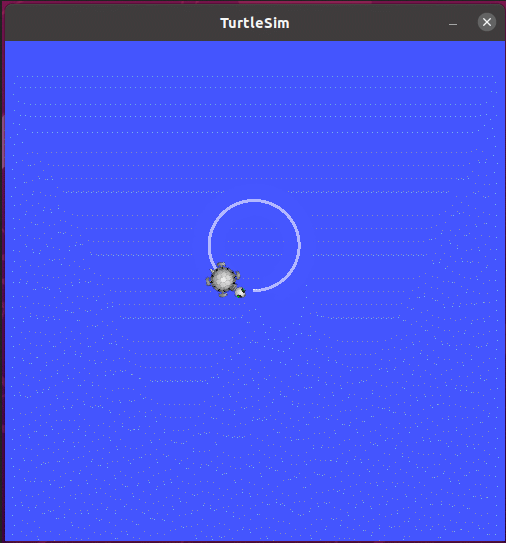
\includegraphics[width=.5\textwidth]{ros_demo_publish_topic.png}
  \caption{话题发布结果演示}
  \label{fig:ros_demo_publish_topic}
\end{figure}

实现分析: 乌龟运动控制实现关键节点有两个: 1) 乌龟运动显示节点 \verb|turtlesim_node|, 2) 控制节点.  二者是订阅发布模式实现通信的, 乌龟运动显示节点直接调用即可, 运动控制节点之前是使用的 \verb|turtle_teleop_key| 通过键盘 控制, 现在需要自定义控制节点. 控制节点自实现时, 首先需要了解控制节点与显示节点通信使用的话题与消息, 可以使用 ROS 命令结合计算图来获取. 了解了话题与消息之后, 通过 C++ 或 Python 编写运动控制节点, 通过指定的话题, 按照一定的逻辑发布消息即可.

实现流程:

\begin{itemize}
  \item 通过计算图结合 ROS 命令获取话题与消息信息;
  \item 编码实现运动控制节点;
  \item 启动 \verb|roscore|、\verb|turtlesim_node| 以及自定义的控制节点, 查看运行结果.
\end{itemize}

1. 话题与消息获取

准备: 先启动键盘控制乌龟运动案例.

1.1 话题获取

获取话题: \verb|/turtle1/cmd_vel|

通过计算图查看话题, 启动计算图:

\begin{bash}
  rqt_graph
\end{bash}

或者通过 \verb|rostopic| 列出话题:

\begin{bash}
  rostopic list
\end{bash}

1.2 消息获取

获取消息类型: \verb|geometry_msgs/Twist|

\begin{bash}
  rostopic type /turtle1/cmd_vel
\end{bash}

获取消息格式:

\begin{bash}
  rosmsg info geometry_msgs/Twist
\end{bash}

响应结果:

\begin{bash}
  geometry_msgs/Vector3 linear
    float64 x
    float64 y
    float64 z
  geometry_msgs/Vector3 angular
    float64 x
    float64 y
    float64 z
\end{bash}

linear (线速度) 下的 \verb|x, y, z| 分别对应在 $x$、$y$ 和 $z$ 方向上的速度 (单位是 m/s); angular (角速度)下的 \verb|x, y, z| 分别对应 $x$ 轴上的翻滚、$y$ 轴上俯仰和 $z$ 轴上偏航的速度 (单位是rad/s).

2. 实现发布节点

创建功能包需要依赖的功能包: 

\begin{bash}
  catkin_create_pkg your_ros_package roscpp rospy std_msgs geometry_msgs
\end{bash}

实现方案A: C++

\begin{cpp}
  /*
      编写 ROS 节点, 控制小乌龟画圆

      准备工作:
          1. 获取 topic (已知: /turtle1/cmd_vel)
          2. 获取消息类型 (已知: geometry_msgs/Twist)
          3. 运行前, 注意先启动 turtlesim_node 节点

      实现流程:
          1. 包含头文件
          2. 初始化 ROS 节点
          3. 创建发布者对象
          4. 循环发布运动控制消息
  */

  #include "ros/ros.h"
  #include "geometry_msgs/Twist.h"

  int main(int argc, char *argv[])
  {
      setlocale(LC_ALL,"");
      // 2. 初始化 ROS 节点
      ros::init(argc,argv,"control");
      ros::NodeHandle nh;
      // 3. 创建发布者对象
      ros::Publisher pub = nh.advertise<geometry_msgs::Twist>("/turtle1/cmd_vel",1000);
      // 4. 循环发布运动控制消息
      // 4-1. 组织消息
      geometry_msgs::Twist msg;
      msg.linear.x = 1.0;
      msg.linear.y = 0.0;
      msg.linear.z = 0.0;

      msg.angular.x = 0.0;
      msg.angular.y = 0.0;
      msg.angular.z = 2.0;

      // 4-2. 设置发送频率
      ros::Rate r(10);
      // 4-3. 循环发送
      while (ros::ok())
      {
          pub.publish(msg);

          ros::spinOnce();
      }


      return 0;
  }
\end{cpp}

配置文件此处略

实现方案B: Python

\begin{python}
  #! /usr/bin/env python
  """
      编写 ROS 节点, 控制小乌龟画圆

      准备工作:
          1. 获取topic(已知: /turtle1/cmd_vel)
          2. 获取消息类型 (已知: geometry_msgs/Twist)
          3. 运行前, 注意先启动 turtlesim_node 节点

      实现流程:
          1. 导包
          2. 初始化 ROS 节点
          3. 创建发布者对象
          4. 循环发布运动控制消息
  """

  import rospy
  from geometry_msgs.msg import Twist

  if __name__ == "__main__":
      # 2. 初始化 ROS 节点
      rospy.init_node("control_circle_p")
      # 3. 创建发布者对象
      pub = rospy.Publisher("/turtle1/cmd_vel",Twist,queue_size=1000)
      # 4. 循环发布运动控制消息
      rate = rospy.Rate(10)
      msg = Twist()
      msg.linear.x = 1.0
      msg.linear.y = 0.0
      msg.linear.z = 0.0
      msg.angular.x = 0.0
      msg.angular.y = 0.0
      msg.angular.z = 0.5

      while not rospy.is_shutdown():
          pub.publish(msg)
          rate.sleep()
\end{python}

权限设置以及配置文件此处略.

3. 运行

\begin{itemize}
  \item 首先, 启动 \verb|roscore|; 
  \item 然后启动乌龟显示节点; 
  \item 最后执行运动控制节点; 
  \item 最终执行结果与演示结果类似.
\end{itemize}

\subsection{话题订阅}

需求描述: 已知 \verb|turtlesim| 中的乌龟显示节点, 会发布当前乌龟的位姿 (窗体中乌龟的坐标以及朝向), 要求控制乌龟运动, 并时时打印当前乌龟的位姿.

结果演示如图 \ref{fig:ros_demo_subscribe_topic} 所示.

\begin{figure}[!ht]
  \centering
  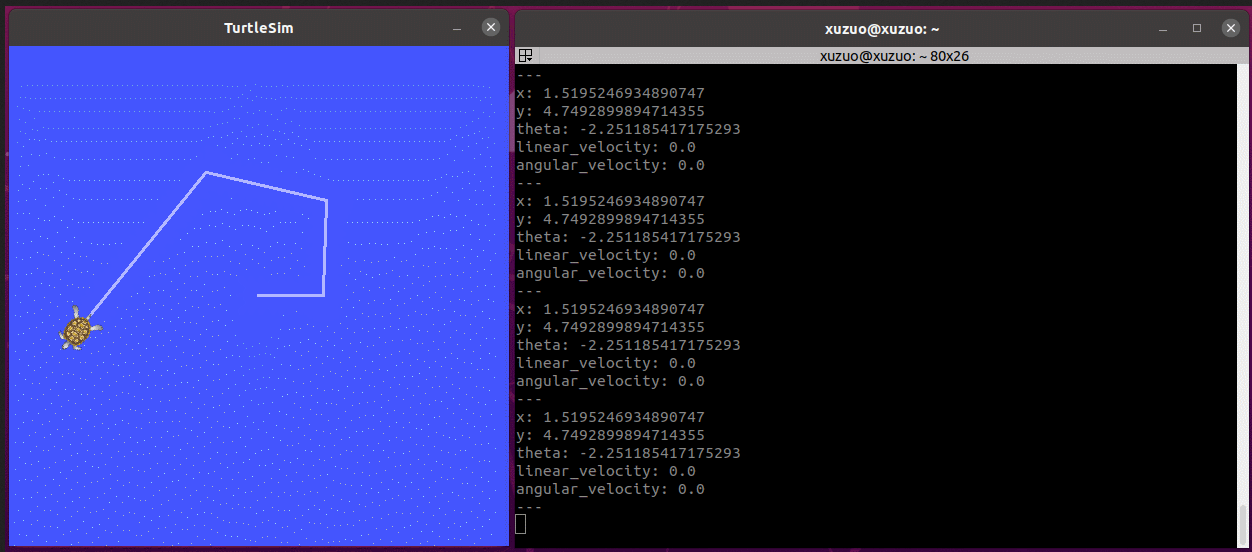
\includegraphics[width=.9\textwidth]{ros_demo_subscribe_topic.png}
  \caption{话题订阅结果演示}
  \label{fig:ros_demo_subscribe_topic}
\end{figure}

实现分析: 首先, 需要启动乌龟显示以及运动控制节点并控制乌龟运动. 要通过 ROS 命令, 来获取乌龟位姿发布的话题以及消息. 编写订阅节点, 订阅并打印乌龟的位姿.

实现流程:

\begin{itemize}
  \item 通过 ROS 命令获取话题与消息信息;
  \item 编码实现位姿获取节点;
  \item 启动 \verb|roscore|、\verb|turtlesim_node|、控制节点以及位姿订阅节点, 控制乌龟运动并输出乌龟的位姿.
\end{itemize}

1. 话题与消息获取

获取话题: \verb|/turtle1/pose|

\begin{bash}
  rostopic list
\end{bash}

获取消息类型: \verb|turtlesim/Pose|

\begin{bash}
  rostopic type  /turtle1/pose
\end{bash}

获取消息格式:

\begin{bash}
  rosmsg info turtlesim/Pose
\end{bash}

响应结果:

\begin{bash}
  float32 x
  float32 y
  float32 theta
  float32 linear_velocity
  float32 angular_velocity
\end{bash}

2. 实现订阅节点

创建功能包需要依赖的功能包: 

\begin{bash}
  catkin_create_pkg your_ros_package roscpp rospy std_msgs turtlesim
\end{bash}

实现方案A: C++

\begin{cpp}
  /*  
      订阅小乌龟的位姿: 时时获取小乌龟在窗体中的坐标并打印
      准备工作:
          1. 获取话题名称 /turtle1/pose
          2. 获取消息类型 turtlesim/Pose
          3. 运行前启动 turtlesim_node 与 turtle_teleop_key 节点

      实现流程:
          1. 包含头文件
          2. 初始化 ROS 节点
          3. 创建 ROS 句柄
          4. 创建订阅者对象
          5. 回调函数处理订阅的数据
          6. spin
  */

  #include "ros/ros.h"
  #include "turtlesim/Pose.h"

  void doPose(const turtlesim::Pose::ConstPtr& p){
      ROS_INFO("乌龟位姿信息:x=%.2f,y=%.2f,theta=%.2f,lv=%.2f,av=%.2f",
          p->x,p->y,p->theta,p->linear_velocity,p->angular_velocity
      );
  }

  int main(int argc, char *argv[])
  {
      setlocale(LC_ALL,"");
      // 2. 初始化 ROS 节点
      ros::init(argc,argv,"sub_pose");
      // 3. 创建 ROS 句柄
      ros::NodeHandle nh;
      // 4. 创建订阅者对象
      ros::Subscriber sub = nh.subscribe<turtlesim::Pose>("/turtle1/pose",1000,doPose);
      // 5. 回调函数处理订阅的数据
      // 6. spin
      ros::spin();
      return 0;
  }
\end{cpp}

配置文件此处略

实现方案B: Python

\begin{python}
  #! /usr/bin/env python
  """
      订阅小乌龟的位姿: 时时获取小乌龟在窗体中的坐标并打印
      准备工作:
          1. 获取话题名称 /turtle1/pose
          2. 获取消息类型 turtlesim/Pose
          3. 运行前启动 turtlesim_node 与 turtle_teleop_key 节点

      实现流程:
          1. 导包
          2. 初始化 ROS 节点
          3. 创建订阅者对象
          4. 回调函数处理订阅的数据
          5. spin

  """

  import rospy
  from turtlesim.msg import Pose

  def doPose(data):
      rospy.loginfo("乌龟坐标:x=%.2f, y=%.2f,theta=%.2f",data.x,data.y,data.theta)

  if __name__ == "__main__":

      # 2. 初始化 ROS 节点
      rospy.init_node("sub_pose_p")

      # 3. 创建订阅者对象
      sub = rospy.Subscriber("/turtle1/pose",Pose,doPose,queue_size=1000)
      #     4. 回调函数处理订阅的数据
      #     5. spin
      rospy.spin()
\end{python}

权限设置以及配置文件此处略.

3. 运行

\begin{itemize}
  \item 首先, 启动 \verb|roscore|;
  \item 然后启动乌龟显示节点, 执行运动控制节点; 
  \item 最后启动乌龟位姿订阅节点; 
  \item 最终执行结果与演示结果类似.
\end{itemize}

\subsection{服务调用}

需求描述: 编码实现向 \verb|turtlesim| 发送请求, 在乌龟显示节点的窗体指定位置生成一乌龟, 这是一个服务请求操作.

结果演示如图 \ref{fig:ros_demo_call_srv} 所示.

\begin{figure}[!ht]
  \centering
  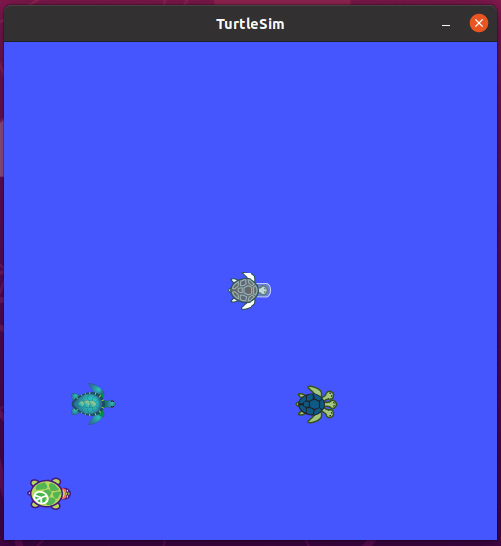
\includegraphics[width=.5\textwidth]{ros_demo_call_srv.png}
  \caption{服务调用结果演示}
  \label{fig:ros_demo_call_srv}
\end{figure}

实现分析: 首先, 需要启动乌龟显示节点. 要通过 ROS 命令, 来获取乌龟生成服务的服务名称以及服务消息类型. 编写服务请求节点, 生成新的乌龟.

实现流程:

\begin{itemize}
  \item 通过 ROS 命令获取服务与服务消息信息.
  \item 编码实现服务请求节点.
  \item 启动 \verb|roscore|、\verb|turtlesim_node|、乌龟生成节点, 生成新的乌龟.
\end{itemize}

1. 服务名称与服务消息获取

获取话题: \verb|/spawn|

\begin{bash}
  rosservice list
\end{bash}

获取消息类型: \verb|turtlesim/Spawn|

\begin{bash}
  rosservice type /spawn
\end{bash}

获取消息格式:

\begin{bash}
  rossrv info turtlesim/Spawn
\end{bash}

响应结果:

\begin{bash}
  float32 x
  float32 y
  float32 theta
  string name
  ---
  string name
\end{bash}

2. 服务客户端实现

创建功能包需要依赖的功能包:

\begin{bash}
  catkin_create_pkg your_ros_package roscpp rospy std_msgs turtlesim
\end{bash}

实现方案A: C++

\begin{cpp}
  /**
      生成一只小乌龟
      准备工作:
          1. 服务话题 /spawn
          2. 服务消息类型 turtlesim/Spawn
          3. 运行前先启动 turtlesim_node 节点

      实现流程:
          1. 包含头文件
            需要包含 turtlesim 包下资源, 注意在 package.xml 配置
          2. 初始化 ROS 节点
          3. 创建 ROS 句柄
          4. 创建 service 客户端
          5. 等待服务启动
          6. 发送请求
          7. 处理响应
   */

  #include "ros/ros.h"
  #include "turtlesim/Spawn.h"

  int main(int argc, char *argv[])
  {
      setlocale(LC_ALL,"");
      // 2. 初始化 ROS 节点
      ros::init(argc,argv,"set_turtle");
      // 3. 创建 ROS 句柄
      ros::NodeHandle nh;
      // 4. 创建 service 客户端
      ros::ServiceClient client = nh.serviceClient<turtlesim::Spawn>("/spawn");
      // 5. 等待服务启动
      // client.waitForExistence();
      ros::service::waitForService("/spawn");
      // 6. 发送请求
      turtlesim::Spawn spawn;
      spawn.request.x = 1.0;
      spawn.request.y = 1.0;
      spawn.request.theta = 1.57;
      spawn.request.name = "my_turtle";
      bool flag = client.call(spawn);
      // 7. 处理响应结果
      if (flag)
      {
          ROS_INFO("新的乌龟生成, 名字:%s",spawn.response.name.c_str());
      } else {
          ROS_INFO("乌龟生成失败!!!");
      }
      return 0;
  }
\end{cpp}

配置文件此处略.

实现方案B: Python

\begin{python}
  #! /usr/bin/env python
  """
      生成一只小乌龟
      准备工作:
          1. 服务话题 /spawn
          2. 服务消息类型 turtlesim/Spawn
          3. 运行前先启动 turtlesim_node 节点

      实现流程:
          1. 导包
            需要包含 turtlesim 包下资源, 注意在 package.xml 配置
          2. 初始化 ROS 节点
          3. 创建 service 客户端
          4. 等待服务启动
          5. 发送请求
          6. 处理响应
  """

  import rospy
  from turtlesim.srv import Spawn,SpawnRequest,SpawnResponse

  if __name__ == "__main__":
      # 2. 初始化 ROS 节点
      rospy.init_node("set_turtle_p")
      # 3. 创建 service 客户端
      client = rospy.ServiceProxy("/spawn",Spawn)
      # 4. 等待服务启动
      client.wait_for_service()
      # 5. 发送请求
      req = SpawnRequest()
      req.x = 2.0
      req.y = 2.0
      req.theta = -1.57
      req.name = "my_turtle_p"
      try:
          response = client.call(req)
          # 6. 处理响应
          rospy.loginfo("乌龟创建成功!, 叫:%s",response.name)
      except expression as identifier:
          rospy.loginfo("服务调用失败")
\end{python}

权限设置以及配置文件此处略.

3. 运行

\begin{itemize}
  \item 首先, 启动 \verb|roscore|;
  \item 然后启动乌龟显示节点; 
  \item 最后启动乌龟生成请求节点; 
  \item 最终执行结果与演示结果类似.
\end{itemize}

\subsection{参数设置}

需求描述: 修改 \verb|turtlesim| 乌龟显示节点窗体的背景色, 已知背景色是通过参数服务器的方式以 RGB 方式设置的.

结果演示如图 \ref{fig:ros_demo_set_param} 所示.

\begin{figure}[!ht]
  \centering
  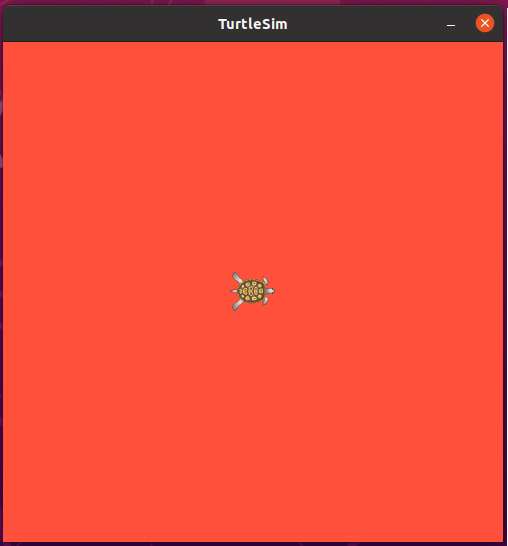
\includegraphics[width=.5\textwidth]{ros_demo_set_param.png}
  \caption{参数设置结果演示}
  \label{fig:ros_demo_set_param}
\end{figure}

实现分析: 首先, 需要启动乌龟显示节点. 要通过 ROS 命令, 来获取参数服务器中设置背景色的参数. 编写参数设置节点, 修改参数服务器中的参数值.

实现流程:

\begin{itemize}
  \item 通过 ROS 命令获取参数.
  \item 编码实现服参数设置节点.
  \item 启动 \verb|roscore|、\verb|turtlesim_node| 与参数设置节点, 查看运行结果.
\end{itemize}

1. 参数名获取

获取参数列表:

\begin{bash}
  rosparam list
\end{bash}

响应结果:

\begin{bash}
  /turtlesim/background_b
  /turtlesim/background_g
  /turtlesim/background_r
\end{bash}

2. 参数修改

实现方案A: C++

\begin{cpp}
  /*
      注意命名空间的使用.
   */

  #include "ros/ros.h"

  int main(int argc, char *argv[])
  {
      ros::init(argc,argv,"haha");

      ros::NodeHandle nh("turtlesim");
      //ros::NodeHandle nh;

      // ros::param::set("/turtlesim/background_r",0);
      // ros::param::set("/turtlesim/background_g",0);
      // ros::param::set("/turtlesim/background_b",0);

      nh.setParam("background_r",0);
      nh.setParam("background_g",0);
      nh.setParam("background_b",0);

      return 0;
  }
\end{cpp}

配置文件此处略.

实现方案B: Python

\begin{python}
  #! /usr/bin/env python

  import rospy

  if __name__ == "__main__":
      rospy.init_node("hehe")
      # rospy.set_param("/turtlesim/background_r",255)
      # rospy.set_param("/turtlesim/background_g",255)
      # rospy.set_param("/turtlesim/background_b",255)
      rospy.set_param("background_r",255)
      rospy.set_param("background_g",255)
      rospy.set_param("background_b",255)  # 调用时, 需要传入 __ns:=xxx
\end{python}

权限设置以及配置文件此处略.

3. 运行

\begin{itemize}
  \item 首先, 启动 \verb|roscore|;
  \item 然后启动背景色设置节点; 
  \item 最后启动乌龟显示节点; 
  \item 最终执行结果与演示结果类似.
\end{itemize}

PS: 注意节点启动顺序, 如果先启动乌龟显示节点, 后启动背景色设置节点, 那么颜色设置不会生效.

4. 其他设置方式

方式1: 修改小乌龟节点的背景色 (命令行实现).

\begin{bash}
  rosparam set /turtlesim/background_b 自定义数值
  rosparam set /turtlesim/background_g 自定义数值
  rosparam set /turtlesim/background_r 自定义数值
\end{bash}

修改相关参数后, 重启 \verb|turtlesim_node| 节点, 背景色就会发生改变了

方式2: 启动节点时, 直接设置参数.

\begin{bash}
  rosrun turtlesim turtlesim_node _background_r:=100 _background_g=0 _background_b=0
\end{bash}

方式3: 通过launch文件传参.

\begin{xml}
  <launch>
      <node pkg="turtlesim" type="turtlesim_node" name="set_bg" output="screen">
          <!-- launch 传参策略1 -->
          <!-- <param name="background_b" value="0" type="int" />
          <param name="background_g" value="0" type="int" />
          <param name="background_r" value="0" type="int" /> -->

          <!-- launch 传参策略2 -->
          <rosparam command="load" file="$(find demo03_test_parameter)/cfg/color.yaml" />
      </node>
  </launch>
\end{xml}

\section{通信机制比较}

三种通信机制中, 参数服务器是一种数据共享机制, 可以在不同的节点之间共享数据, 话题通信与服务通信是在不同的节点之间传递数据的, 三者是 ROS 中最基础也是应用最为广泛的通信机制.

这其中, 话题通信和服务通信有一定的相似性也有本质上的差异, 在此将二者做一下简单比较: 二者的实现流程是比较相似的, 都是涉及到四个要素:

\begin{itemize}
  \item 消息的发布方/客户端 (Publisher/Client)
  \item 消息的订阅方/服务端 (Subscriber/Server)
  \item 话题名称 (Topic/Service)
  \item 数据载体 (msg/srv)
\end{itemize}

可以概括为: 两个节点通过话题关联到一起, 并使用某种类型的数据载体实现数据传输. 二者的实现也是有本质差异的, 具体比较如下:

\begin{table}[!ht]
  \centering
  \caption{通信机制比较}
  \label{tab:communication_mechanism_comparison}
  \begin{tabular}{lp{4cm}p{4.5cm}}
    \hline
    & Topic (话题)  &	Service (服务) \\
    \hline
    通信模式 & 发布/订阅 	      & 请求/响应 \\
    同步性 	 & 异步 	          & 同步 \\
    底层协议 & ROSTCP/ROSUDP 	  & ROSTCP/ROSUDP \\
    缓冲区 	 & 有 	            & 无 \\
    时时性 	 & 弱 	            & 强 \\
    节点关系 & 多对多 	        &   一对多 (一个 Server) \\
    通信数据 & msg 	            &   srv \\
    使用场景 & 连续高频的数据发布与接收: 雷达、里程计 &	偶尔调用或执行某一项特定功能: 拍照、语音识别 \\
    \hline
  \end{tabular}
\end{table}

不同通信机制有一定的互补性, 都有各自适应的应用场景. 尤其是话题与服务通信, 需要结合具体的应用场景与二者的差异, 选择合适的通信机制.

\section{本章小结}

本章主要介绍了 ROS 中最基本的也是最核心的通信机制实现: 话题通信、服务通信、参数服务器. 每种通信机制, 都介绍了如下内容:

\begin{itemize}
  \item 介绍了当前通信机制的应用场景; 
  \item 介绍了当前通信机制的理论模型; 
  \item 分别介绍了当前通信机制的 C++ 与 Python 实现.
\end{itemize}

除此之外, 还介绍了:

\begin{itemize}
  \item ROS 中的常用命令方便操作、调试节点以及通信信息; 
  \item 通过实操又将上述知识点加以整合; 
  \item 最后又着重比较了话题通信与服务通信的相同点以及差异.
\end{itemize}

掌握本章内容后, 基本上就可以从容应对 ROS 中大部分应用场景了.

\chapter{ROS通信机制进阶}
\label{chapter:ros_communication_advanced}

上一章内容, 主要介绍了 ROS 通信的实现, 内容偏向于粗粒度的通信框架的讲解, 没有详细介绍涉及的 API, 也没有封装代码, 鉴于此, 本章主要内容如下:

\begin{itemize}
  \item ROS 常用 API 介绍; 
  \item ROS 中自定义头文件与源文件的使用.
\end{itemize}

预期达成的学习目标:

\begin{itemize}
  \item 熟练掌握 ROS 常用 API; 
  \item 掌握 ROS 中自定义头文件与源文件的配置.
\end{itemize}

\section{常用API}

首先, 建议参考官方 API 文档或参考源码:

\begin{itemize}
  \item ROS 节点的初始化相关 API;
  \item NodeHandle 的基本使用相关 API;
  \item 话题的发布方, 订阅方对象相关 API;
  \item 服务的服务端, 客户端对象相关 API;
  \item 时间相关 API;
  \item 日志输出相关 API.
\end{itemize}

参数服务器相关 API 在第二章已经有详细介绍和应用, 在此不再赘述.

另请参考:

\begin{itemize}
  \item \href{http://wiki.ros.org/APIs}{ROS/APIs};
  \item \href{https://docs.ros.org/en/api/roscpp/html/}{roscpp api}.
\end{itemize}

\subsection{初始化}

\subsubsection{C++初始化}

\begin{cpp}
  /** @brief ROS初始化函数.
   *
   * 该函数可以解析并使用节点启动时传入的参数 (通过参数设置节点名称、 命名空间...) 
   *
   * 该函数有多个重载版本, 如果使用 NodeHandle 建议调用该版本.  
   *
   * \param argc 参数个数
   * \param argv 参数列表
   * \param name 节点名称, 需要保证其唯一性, 不允许包含命名空间
   * \param options 节点启动选项, 被封装进了ros::init_options
   *
   */
  void init(int &argc, char **argv, const std::string& name, uint32_t options = 0);
\end{cpp}

\subsubsection{Python初始化}

\begin{python}
  def init_node(name, argv=None, anonymous=False, log_level=None, disable_rostime=False, disable_rosout=False, disable_signals=False, xmlrpc_port=0, tcpros_port=0):
      """
      在 ROS msater 中注册节点

      @param name: 节点名称, 必须保证节点名称唯一, 节点名称中不能使用命名空间 (不能包含 '/')
      @type  name: str

      @param anonymous: 取值为 true 时, 为节点名称后缀随机编号
      @type anonymous: bool
      """
\end{python}

\subsection{话题与服务相关对象}

\subsubsection{C++}

在 \verb|roscpp| 中, 话题和服务的相关对象一般由 NodeHandle 创建. NodeHandle 有一个重要作用是可以用于设置命名空间, 这是后期的重点, 但是本章暂不介绍.

1. 发布对象

对象获取:

\begin{cpp}
  /**
   * \brief 根据话题生成发布对象
   *
   * 在 ROS master 注册并返回一个发布者对象, 该对象可以发布消息
   *
   * 使用示例如下:
   *
   *   ros::Publisher pub = handle advertise<std_msgs::Empty>("my_topic", 1);
   *
   * \param topic 发布消息使用的话题
   *
   * \param queue_size 等待发送给订阅者的最大消息数量
   *
   * \param latch (optional) 如果为 true, 该话题发布的最后一 消息将被保存, 并且后期当有订阅者连接时会将该消息发送给订阅者
   *
   * \return 调用成功时, 会返回一个发布对象
   *
   *
   */

  template <class M>
  Publisher advertise(const std::string& topic, uint32_t queue_size, bool latch = false);
\end{cpp}

消息发布函数:

\begin{cpp}
  /**
   * 发布消息          
   */

  template <typename M>
  void publish(const M& message) const;
\end{cpp}

2. 订阅对象

对象获取:

\begin{cpp}
  /**
   * \brief 生成某个话题的订阅对象
   *
   * 该函数将根据给定的话题在ROS master 注册, 并自动连接相同主 的发布方, 每接收到一条消息, 都会调用回调
   * 函数, 并且传入该消息的共享指针, 该消息不能被修改, 因为可能 他订阅对象也会使用该消息.
   * 
   * 使用示例如下:
   \verbatim
   void callback(const std_msgs::Empty::ConstPtr& message)
   {
   } 
   ros::Subscriber sub = handle.subscribe("my_topic", 1, callback);
   \endverbatim
   *
   * \param M [template] M 是指消息类型
   * \param topic 订阅的话题
   * \param queue_size 消息队列长度, 超出长度时, 头部的消息将 弃用
   * \param fp 当订阅到一条消息时, 需要执行的回调函数
   * \return 调用成功时, 返回一个订阅者对象, 失败时, 返回空对象
   * 
   \verbatim
   void callback(const std_msgs::Empty::ConstPtr& message){...}
   ros::NodeHandle nodeHandle;
   ros::Subscriber sub = nodeHandle.subscrib ("my_topic", 1, callback);
   if (sub) // Enter if subscriber is valid
   {
   ...
   }
   \endverbatim
   */

  template<class M>
  Subscriber subscribe(const std::string& topic, uint32_t queue_size, void(*fp)(const boost::shared_ptr<M const>&), const TransportHints& transport_hints = TransportHints());
\end{cpp}

3. 服务对象

对象获取:

\begin{cpp}
  /**
   * \brief 生成服务端对象
   *
   * 该函数可以连接到 ROS master, 并提供一个具有给定名称的服务 象.
   *
   * 使用示例如下:
   \verbatim
   bool callback(std_srvs::Empty& request, std_srvs::Empty& response)
   {
   return true;
   } 
   ros::ServiceServer service = handle.advertiseServic ("my_service", callback);
   \endverbatim
   *
   * \param service 服务的主题名称
   * \param srv_func 接收到请求时, 需要处理请求的回调函数
   * \return 请求成功时返回服务对象, 否则返回空对象:
   \verbatim
   bool Foo::callback(std_srvs::Empty& request, std_srvs::Empty& response)
   {
   return true;
   }
   ros::NodeHandle nodeHandle;
   Foo foo_object;
   ros::ServiceServer service = nodeHandle advertiseService("my_service", callback);
   if (service) // Enter if advertised service is valid
   {
   ...
   }
   \endverbatim 
   */

  template<class MReq, class MRes>
  ServiceServer advertiseService(const std::string& service, bool(*srv_func)(MReq&, MRes&));
\end{cpp}

4. 客户端对象

对象获取:

\begin{cpp}
  /** 
   * @brief 创建一个服务客户端对象
   *
   * 当清除最后一个连接的引用句柄时, 连接将被关闭.
   *
   * @param service_name 服务主题名称
   */

  template<class Service>
  ServiceClient serviceClient(const std::string& service_name, bool persistent = false, 
                              const M_string& header_values = M_string());
\end{cpp}

请求发送函数:

\begin{cpp}
  /**
   * @brief 发送请求
   * 返回值为 bool 类型, true, 请求处理成功, false, 处理失败.
   */
    
    template<class Service>
    bool call(Service& service);
\end{cpp}

等待服务函数1:

\begin{cpp}
  /**
   * ros::service::waitForService("addInts");
   * \brief 等待服务可用, 否则一致处于阻塞状态
   * \param service_name 被"等待"的服务的话题名称
   * \param timeout 等待最大时常, 默认为 -1, 可以永久等待直至节点 关闭
   * \return 成功返回 true, 否则返回 false.
   */

  ROSCPP_DECL bool waitForService(const std::string& service_name, ros::Duration timeout = ros::Duration(-1));
\end{cpp}

等待服务函数2:

\begin{cpp}
  /**
   * client.waitForExistence();
   * \brief 等待服务可用, 否则一致处于阻塞状态
   * \param timeout 等待最大时常, 默认为 -1, 可以永久等待直至节点 关闭
   * \return 成功返回 true, 否则返回 false.
   */

  bool waitForExistence(ros::Duration timeout = ros::Duration(-1));
\end{cpp}

\subsubsection{Python}

1. 发布对象

对象获取:

\begin{python}
  class Publisher(Topic):
      """
      在ROS master注册为相关话题的发布方
      """

      def __init__(self, name, data_class, subscriber_listener=None, tcp_nodelay=False, latch=False, headers=None, queue_size=None):
          """
          Constructor
          @param name: 话题名称 
          @type  name: str
          @param data_class: 消息类型

          @param latch: 如果为 true, 该话题发布的最后一条消息将被保存, 并且后期当有订阅者连接时会将该消息发送给订阅者
          @type  latch: bool

          @param queue_size: 等待发送给订阅者的最大消息数量
          @type  queue_size: int

          """
\end{python}

消息发布函数:

\begin{python}
  def publish(self, *args, **kwds):
          """
          发布消息
          """
\end{python}

2. 订阅对象

对象获取:

\begin{python}
  class Subscriber(Topic):
      """
    类注册为指定主题的订阅者, 其中消息是给定类型的.
      """
      def __init__(self, name, data_class, callback=None, callback_args=None,
                  queue_size=None, buff_size=DEFAULT_BUFF_SIZE, tcp_nodelay=False):
          """
          Constructor.

          @param name: 话题名称
          @type  name: str
          @param data_class: 消息类型
          @type  data_class: L{Message} class
          @param callback: 处理订阅到的消息的回调函数
          @type  callback: fn(msg, cb_args)

          @param queue_size: 消息队列长度, 超出长度时, 头部的消息将被弃用

          """
\end{python}

3. 服务对象

对象获取:

\begin{python}
  class Service(ServiceImpl):
      """
      声明一个 ROS 服务

      使用示例::
        s = Service('getmapservice', GetMap, get_map_handler)
      """

      def __init__(self, name, service_class, handler,
                  buff_size=DEFAULT_BUFF_SIZE, error_handler=None):
          """

          @param name: 服务主题名称 ``str``
          @param service_class:服务消息类型

          @param handler: 回调函数, 处理请求数据, 并返回响应数据

          @type  handler: fn(req)->resp

          """
\end{python}

4. 客户端对象

对象获取:

\begin{python}
  class ServiceProxy(_Service):
      """
    创建一个 ROS 服务的句柄

      示例用法::
        add_two_ints = ServiceProxy('add_two_ints', AddTwoInts)
        resp = add_two_ints(1, 2)
      """

      def __init__(self, name, service_class, persistent=False, headers=None):
          """
          ctor.
          @param name: 服务主题名称
          @type  name: str
          @param service_class: 服务消息类型
          @type  service_class: Service class
          """
\end{python}

请求发送函数:

\begin{python}
  def call(self, *args, **kwds):
          """
          发送请求, 返回值为响应数据
          """
\end{python}

等待服务函数:

\begin{python}
  def wait_for_service(service, timeout=None):
      """
      调用该函数时, 程序会处于阻塞状态直到服务可用
      @param service: 被等待的服务话题名称
      @type  service: str
      @param timeout: 超时时间
      @type  timeout: double|rospy.Duration
      """
\end{python}

\subsection{回旋函数}

\subsubsection{C++}

在 ROS 程序中, 频繁的使用了 \verb|ros::spin()| 和 \verb|ros::spinOnce()| 两个回旋函数, 可以用于处理回调函数.

1. \verb|spinOnce()|

\begin{cpp}
  /**
   * \brief 处理一轮回调
   *
   * 一般应用场景:
   *     在循环体内, 处理所有可用的回调函数
   * 
   */

  ROSCPP_DECL void spinOnce();
\end{cpp}

2. \verb|spin()|
\begin{cpp}
  /** 
   * \brief 进入循环处理回调 
   */
  
  ROSCPP_DECL void spin();
\end{cpp}

3. 二者比较

相同点: 二者都用于处理回调函数; 

不同点: \verb|ros::spin()| 是进入了循环执行回调函数, 而 \verb|ros::spinOnce()| 只会执行一次回调函数 (没有循环), 在 \verb|ros::spin()| 后的语句不会执行到, 而 \verb|ros::spinOnce()| 后的语句可以执行.

\subsubsection{Python}

\begin{python}
  def spin():
      """
      进入循环处理回调 
      """
\end{python}

\subsection{时间}

ROS 中时间相关的 API 是极其常用, 比如: 获取当前时刻、持续时间的设置、执行频率、休眠、定时器等等都与时间相关.

\subsubsection{C++}

1. 时刻

获取时刻, 或是设置指定时刻:

\begin{cpp}
  ros::init(argc,argv,"hello_time");
  ros::NodeHandle nh; // 必须创建句柄, 否则时间没有初始化, 导致后续API调用失败
  ros::Time right_now = ros::Time::now(); // 将当前时刻封装成对象
  ROS_INFO("当前时刻:%.2f",right_now.toSec()); // 获取距离 1970年01月01日 00:00:00 的秒数
  ROS_INFO("当前时刻:%d",right_now.sec); // 获取距离 1970年01月01日 00:00:00 的秒数

  ros::Time someTime(100,100000000);// 参数1:秒数  参数2:纳秒
  ROS_INFO("时刻:%.2f",someTime.toSec()); // 100.10
  ros::Time someTime2(100.3);// 直接传入 double 类型的秒数
  ROS_INFO("时刻:%.2f",someTime2.toSec()); // 100.30
\end{cpp}

2. 持续时间

设置一个时间区间 (间隔):

\begin{cpp}
  ROS_INFO("当前时刻:%.2f",ros::Time::now().toSec());
  ros::Duration du(10);// 持续10秒钟, 参数是double类型的, 以秒为单位
  du.sleep();// 按照指定的持续时间休眠
  ROS_INFO("持续时间:%.2f",du.toSec());// 将持续时间换算成秒
  ROS_INFO("当前时刻:%.2f",ros::Time::now().toSec());
\end{cpp}

3. 持续时间与时刻运算

为了方便使用, ROS中提供了时间与时刻的运算:

\begin{cpp}
  ROS_INFO("时间运算");
  ros::Time now = ros::Time::now();
  ros::Duration du1(10);
  ros::Duration du2(20);
  ROS_INFO("当前时刻:%.2f",now.toSec());
  // 1. time 与 duration 运算
  ros::Time after_now = now + du1;
  ros::Time before_now = now - du1;
  ROS_INFO("当前时刻之后:%.2f",after_now.toSec());
  ROS_INFO("当前时刻之前:%.2f",before_now.toSec());

  // 2. duration 之间相互运算
  ros::Duration du3 = du1 + du2;
  ros::Duration du4 = du1 - du2;
  ROS_INFO("du3 = %.2f",du3.toSec());
  ROS_INFO("du4 = %.2f",du4.toSec());
  // PS: time 与 time 不可以运算
  // ros::Time nn = now + before_now; // 异常
\end{cpp}

4. 设置运行频率

\begin{cpp}
  ros::Rate rate(1); // 指定频率
  while (true)
  {
      ROS_INFO("-----------code----------");
      rate.sleep(); // 休眠, 休眠时间 = 1 / 频率.
  }
\end{cpp}

5. 定时器

ROS 中内置了专门的定时器, 可以实现与 \verb|ros::Rate| 类似的效果:

\begin{cpp}
  ros::NodeHandle nh;// 必须创建句柄, 否则时间没有初始化, 导致后续API调用失败

  // ROS 定时器
  /**
   * \brief 创建一个定时器, 按照指定频率调用回调函数.
   *
   * \param period 时间间隔
   * \param callback 回调函数
   * \param oneshot 如果设置为 true, 只执行一次回调函数, 设置为  false, 就循环执行.
   * \param autostart 如果为true, 返回已经启动的定时器, 设置为 false, 需要手动启动.
   */

  //Timer createTimer(Duration period, const TimerCallback& callback, bool oneshot = false,
  //                bool autostart = true) const;

  // ros::Timer timer = nh.createTimer(ros::Duration(0.5),doSomeThing);
  ros::Timer timer = nh.createTimer(ros::Duration(0.5),doSomeThing,true); // 只执行一次

  // ros::Timer timer = nh.createTimer(ros::Duration(0.5),doSomeThing,false,false);// 需要手动启动
  // timer.start();
  ros::spin(); // 必须 spin
\end{cpp}

定时器的回调函数:

\begin{cpp}
  void doSomeThing(const ros::TimerEvent &event){
      ROS_INFO("-------------");
      ROS_INFO("event:%s",std::to_string(event.current_real.toSec()).c_str());
  }
\end{cpp}

\subsubsection{Python}

1. 时刻

获取时刻, 或是设置指定时刻:

\begin{python}
  # 获取当前时刻
  right_now = rospy.Time.now()
  rospy.loginfo("当前时刻:%.2f",right_now.to_sec())
  rospy.loginfo("当前时刻:%.2f",right_now.to_nsec())
  # 自定义时刻
  some_time1 = rospy.Time(1234.567891011)
  some_time2 = rospy.Time(1234,567891011)
  rospy.loginfo("设置时刻1:%.2f",some_time1.to_sec())
  rospy.loginfo("设置时刻2:%.2f",some_time2.to_sec())

  # 从时间创建对象
  # some_time3 = rospy.Time.from_seconds(543.21)
  some_time3 = rospy.Time.from_sec(543.21) # from_sec 替换了 from_seconds
  rospy.loginfo("设置时刻3:%.2f",some_time3.to_sec())
\end{python}

2. 持续时间

设置一个时间区间 (间隔):

\begin{python}
  # 持续时间相关API
  rospy.loginfo("持续时间测试开始.....")
  du = rospy.Duration(3.3)
  rospy.loginfo("du1 持续时间:%.2f",du.to_sec())
  rospy.sleep(du) # 休眠函数
  rospy.loginfo("持续时间测试结束.....")
\end{python}

3. 持续时间与时刻运算

为了方便使用, ROS中提供了时间与时刻的运算:

\begin{python}
  rospy.loginfo("时间运算")
  now = rospy.Time.now()
  du1 = rospy.Duration(10)
  du2 = rospy.Duration(20)
  rospy.loginfo("当前时刻:%.2f",now.to_sec())
  before_now = now - du1
  after_now = now + du1
  dd = du1 + du2
  # now = now + now # 非法
  rospy.loginfo("之前时刻:%.2f",before_now.to_sec())
  rospy.loginfo("之后时刻:%.2f",after_now.to_sec())
  rospy.loginfo("持续时间相加:%.2f",dd.to_sec())
\end{python}

4. 设置运行频率

\begin{python}
  # 设置执行频率
  rate = rospy.Rate(0.5)
  while not rospy.is_shutdown():
      rate.sleep() # 休眠
      rospy.loginfo("+++++++++++++++")
\end{python}

5. 定时器

ROS 中内置了专门的定时器, 可以实现与 ros::Rate 类似的效果:

\begin{python}
  # 定时器设置
  """    
  def __init__(self, period, callback, oneshot=False, reset=False):
      Constructor.
      @param period: 回调函数的时间间隔
      @type  period: rospy.Duration
      @param callback: 回调函数
      @type  callback: function taking rospy.TimerEvent
      @param oneshot: 设置为True, 就只执行一次, 否则循环执行
      @type  oneshot: bool
      @param reset: if True, timer is reset when rostime moved backward. [default: False]
      @type  reset: bool
  """
  rospy.Timer(rospy.Duration(1),doMsg)
  # rospy.Timer(rospy.Duration(1),doMsg,True) # 只执行一次
  rospy.spin()
\end{python}

回调函数:

\begin{python}
  def doMsg(event):
      rospy.loginfo("+++++++++++")
      rospy.loginfo("当前时刻:%s",str(event.current_real))
\end{python}

\subsection{其他函数}

在发布实现时, 一般会循环发布消息, 循环的判断条件一般由节点状态来控制, C++ 中可以通过 \verb|ros::ok()| 来判断节点状态是否正常, Python 中则通过 \verb|rospy.is_shutdown()| 来实现判断, 导致节点退出的原因主要有如下几种:

\begin{itemize}
  \item 节点接收到了关闭信息, 比如常用的 Ctrl + C 快捷键就是关闭节点的信号; 
  \item 同名节点启动, 导致现有节点退出; 
  \item 程序中的其他部分调用了节点关闭相关的 API (C++ 中是 \verb|ros::shutdown()|, Python 中是 \verb|rospy.signal_shutdown()|).
\end{itemize}

另外, 日志相关的函数也是极其常用的, 在 ROS 中日志被划分成如下级别:

\begin{itemize}
  \item DEBUG (调试): 只在调试时使用, 此类消息不会输出到控制台; 
  \item INFO (信息): 标准消息, 一般用于说明系统内正在执行的操作; 
  \item WARN (警告): 提醒一些异常情况, 但程序仍然可以执行; 
  \item ERROR (错误): 提示错误信息, 此类错误会影响程序运行; 
  \item FATAL (严重错误): 此类错误将阻止节点继续运行.
\end{itemize}

\subsubsection{C++}

1. 节点状态判断

\begin{cpp}
  /** \brief 检查节点是否已经退出
   *
   *  ros::shutdown() 被调用且执行完毕后, 该函数将会返回 false
   *
   * \return true 如果节点还健在, false 如果节点已经火化了.
   */
  bool ok();
\end{cpp}

2. 节点关闭函数

\begin{cpp}
  /**
   *   关闭节点
   */
  void shutdown();
\end{cpp}

3. 日志函数

使用示例

\begin{cpp}
  ROS_DEBUG("hello,DEBUG"); // 不会输出
  ROS_INFO("hello,INFO");   // 默认白色字体
  ROS_WARN("Hello,WARN");   // 默认黄色字体
  ROS_ERROR("hello,ERROR"); // 默认红色字体
  ROS_FATAL("hello,FATAL"); // 默认红色字体
\end{cpp}

\subsubsection{Python}

1. 节点状态判断

\begin{python}
  def is_shutdown():
      """
      @return: True 如果节点已经被关闭
      @rtype: bool
      """
\end{python}

2. 节点关闭函数

\begin{python}
  def signal_shutdown(reason):
      """
      关闭节点
      @param reason: 节点关闭的原因, 是一个字符串
      @type  reason: str
      """

  def on_shutdown(h):
      """
      节点被关闭时调用的函数
      @param h: 关闭时调用的回调函数, 此函数无参
      @type  h: fn()
      """
\end{python}

3. 日志函数

使用示例

\begin{python}
  rospy.logdebug("hello,debug")   # 不会输出
  rospy.loginfo("hello,info")     # 默认白色字体
  rospy.logwarn("hello,warn")     # 默认黄色字体
  rospy.logerr("hello,error")     # 默认红色字体
  rospy.logfatal("hello,fatal")   # 默认红色字体
\end{python}


\section{ROS中的头文件与源文件}

本节主要介绍 ROS 的 C++ 实现中, 如何使用头文件与源文件的方式封装代码, 具体内容如下:

\begin{itemize}
  \item 设置头文件, 可执行文件作为源文件; 
  \item 分别设置头文件, 源文件与可执行文件.
\end{itemize}

在 ROS 中关于头文件的使用, 核心内容在于 \verb|CMakeLists.txt| 文件的配置, 不同的封装方式, 配置上也有差异.

\subsection{自定义头文件调用}

需求: 设计头文件, 可执行文件本身作为源文件.

流程:

\begin{itemize}
  \item 编写头文件; 
  \item 编写可执行文件 (同时也是源文件); 
  \item 编辑配置文件并执行.
\end{itemize}

1. 头文件

在功能包下的 \verb|include/功能包名| 目录下新建头文件: \verb|hello.h|, 示例内容如下:

\begin{cpp}
  #ifndef _HELLO_H
  #define _HELLO_H

  namespace hello_ns{

  class HelloPub {

  public:
      void run();
  };

  }

  #endif
\end{cpp}

注意: 在 VScode 中, 请配置 \verb|.vscode| 下 \verb|c_cpp_properties.json| 的 \verb|includepath| 属性, 以使后续包含头文件时不抛出异常.

\begin{xml}
  "/home/用户/工作空间/src/功能包/include/**"
\end{xml}

2. 可执行文件

在 \verb|src| 目录下新建文件: \verb|hello.cpp|, 示例内容如下:

\begin{cpp}
  #include "ros/ros.h"
  #include "test_head/hello.h"

  namespace hello_ns {

  void HelloPub::run(){
      ROS_INFO("自定义头文件的使用....");
  }

  }

  int main(int argc, char *argv[])
  {
      setlocale(LC_ALL,"");
      ros::init(argc,argv,"test_head_node");
      hello_ns::HelloPub helloPub;
      helloPub.run();
      return 0;
  }
\end{cpp}

3. 配置文件

配置 \verb|CMakeLists.txt| 文件, 头文件相关配置如下:

\begin{bash}
  include_directories(
  include
    ${catkin_INCLUDE_DIRS}
  )
\end{bash}

可执行配置文件配置方式与之前一致:

\begin{bash}
  add_executable(hello src/hello.cpp)

  add_dependencies(hello ${${PROJECT_NAME}_EXPORTED_TARGETS} ${catkin_EXPORTED_TARGETS})

  target_link_libraries(hello
    ${catkin_LIBRARIES}
  )
\end{bash}

最后, 编译并执行, 控制台可以输出自定义的文本信息.

\subsection{自定义源文件调用}

需求: 设计头文件与源文件, 在可执行文件中包含头文件.

流程:

\begin{itemize}
  \item 编写头文件; 
  \item 编写源文件; 
  \item 编写可执行文件; 
  \item 编辑配置文件并执行.
\end{itemize}

1. 头文件

在功能包下的 \verb|include/功能包名| 目录下新建头文件: \verb|haha.h|, 示例内容如下:

\begin{cpp}
  #ifndef _HAHA_H
  #define _HAHA_H

  namespace hello_ns {

  class My {

  public:
      void run();

  };

  }

  #endif
\end{cpp}

2. 源文件

在 \verb|src| 目录下新建文件: \verb|haha.cpp|, 示例内容如下:

\begin{cpp}
  #include "test_head_src/haha.h"
  #include "ros/ros.h"

  namespace hello_ns{

  void My::run(){
      ROS_INFO("hello,head and src ...");
  }

  }
\end{cpp}

3. 可执行文件

在 \verb|src| 目录下新建文件: \verb|use_head.cpp|, 示例内容如下:

\begin{cpp}
  #include "ros/ros.h"
  #include "test_head_src/haha.h"

  int main(int argc, char *argv[])
  {
      ros::init(argc,argv,"hahah");
      hello_ns::My my;
      my.run();
      return 0;
  }
\end{cpp}

4. 配置文件

头文件与源文件相关配置:

\begin{bash}
  include_directories(
  include
    ${catkin_INCLUDE_DIRS}
  )

  ## 声明 C++ 库
  add_library(head
    include/test_head_src/haha.h
    src/haha.cpp
  )

  add_dependencies(head ${${PROJECT_NAME}_EXPORTED_TARGETS} ${catkin_EXPORTED_TARGETS})

  target_link_libraries(head
    ${catkin_LIBRARIES}
  )
\end{bash}

可执行文件配置:

\begin{bash}
  add_executable(use_head src/use_head.cpp)

  add_dependencies(use_head ${${PROJECT_NAME}_EXPORTED_TARGETS} ${catkin_EXPORTED_TARGETS})

  # 此处需要添加之前设置的 head 库
  target_link_libraries(use_head
    head
    ${catkin_LIBRARIES}
  )
\end{bash}

\section{Python模块导入}

与 C++ 类似的, 在 Python 中导入其他模块时, 也需要相关处理.

需求: 首先新建一个 Python 文件A, 再创建 Python 文件UseA, 在 UseA 中导入 A 并调用 A 的实现.

实现:

\begin{itemize}
  \item 新建两个 Python 文件, 使用 \verb|import| 实现导入关系; 
  \item 添加可执行权限、编辑配置文件并执行 UseA.
\end{itemize}

1. 新建两个 Python 文件并使用 \verb|import| 导入

文件 A 实现 (包含一个变量):

\begin{python}
  #! /usr/bin/env python
  num = 1000
\end{python}

文件 B 核心实现:

\begin{python}
  import os
  import sys

  path = os.path.abspath(".")
  # 核心
  sys.path.insert(0,path + "/src/plumbing_pub_sub/scripts")

  import tools

  ....
  ....
      rospy.loginfo("num = %d",tools.num)
\end{python}

2. 添加可执行权限, 编辑配置文件并执行

此过程略.

\section{本章小结}

本章内容相对比较简单, 多加练习即可.

\chapter{ROS运行管理}
\label{chapter:ros_run_management}

ROS是多进程 (节点) 的分布式框架, 一个完整的 ROS 系统实现: 

\begin{itemize}
  \item 可能包含多台主机; 
  \item 每台主机上又有多个工作空间 (workspace); 
  \item 每个的工作空间中又包含多个功能包 (package); 
  \item 每个功能包又包含多个节点 (Node), 不同的节点都有自己的节点名称; 
  \item 每个节点可能还会设置一个或多个话题 (topic).
\end{itemize}

在多级层深的 ROS 系统中, 其实现与维护可能会出现一些问题, 比如, 如何关联不同的功能包, 繁多的 ROS 节点应该如何启动? 功能包、节点、话题、参数重名时应该如何处理? 不同主机上的节点如何通信? 

本章主要内容介绍在 ROS 中上述问题的解决策略 (见本章目录), 预期达成学习目标也与上述问题对应: 

\begin{itemize}
  \item 掌握元功能包使用语法; 
  \item 掌握 launch 文件的使用语法; 
  \item 理解什么是 ROS 工作空间覆盖, 以及存在什么安全隐患; 
  \item 掌握节点名称重名时的处理方式; 
  \item 掌握话题名称重名时的处理方式; 
  \item 掌握参数名称重名时的处理方式; 
  \item 能够实现 ROS 分布式通信.
\end{itemize}

\section{ROS元功能包}

场景: 完成 ROS 中一个系统性的功能, 可能涉及到多个功能包, 比如实现了机器人导航模块, 该模块下有地图、定位、路径规划...等不同的子级功能包. 那么调用者安装该模块时, 需要逐一的安装每一个功能包吗?

显而易见的, 逐一安装功能包的效率低下, 在 ROS 中, 提供了一种方式可以将不同的功能包打包成一个功能包, 当安装某个功能模块时, 直接调用打包后的功能包即可, 该包又称之为元功能包 (Meta Package).

概念: MetaPackage 是 Linux 的一个文件管理系统的概念, 是 ROS 中的一个虚包, 里面没有实质性的内容, 但是它依赖了其他的软件包, 通过这种方法可以把其他包组合起来, 我们可以认为它是一本书的目录索引, 告诉我们这个包集合中有哪些子包, 并且该去哪里下载.

例如: \verb|sudo apt install ros-noetic-desktop-full| 命令安装 ROS 时就使用了元功能包, 该元功能包依赖于 ROS 中的其他一些功能包, 安装该包时会一并安装依赖.

还有一些常见的 MetaPackage: \verb|navigation|, \verb|moveit|, \verb|turtlebot3|...

作用: 方便用户的安装, 我们只需要这一个包就可以把其他相关的软件包组织到一起安装了.

实现:

首先: 新建一个功能包.

然后: 修改 \verb|package.xml|, 内容如下:

\begin{xml}
  <exec_depend>被集成的功能包</exec_depend>
  .....
  <export>
    <metapackage />
  </export>
\end{xml}

最后: 修改 \verb|CMakeLists.txt|, 内容如下:

\begin{bash}
  cmake_minimum_required(VERSION 3.0.2)
  project(demo)
  find_package(catkin REQUIRED)
  catkin_metapackage()
\end{bash}

PS: \verb|CMakeLists.txt| 中不可以有换行.

另请参考: \href{http://wiki.ros.org/catkin/package.xml#Metapackages}{ROS/Metapackages}.

\section{ROS节点运行管理launch文件}

关于 launch 文件的使用我们已经不陌生了, 在第一章内容中, 就曾经介绍到: 一个程序中可能需要启动多个节点, 比如: ROS 内置的小乌龟案例, 如果要控制乌龟运动, 要启动多个窗口, 分别启动 \verb|roscore|、乌龟界面节点、键盘控制节点. 如果每次都调用 \verb|rosrun| 逐一启动, 显然效率低下, 如何优化? 采用的优化策略便是使用 \verb|roslaunch| 命令集合 launch 文件启动管理节点, 并且在后续教程中, 也多次使用到了 launch 文件.

概念: launch 文件是一个 XML 格式的文件, 可以启动本地和远程的多个节点, 还可以在参数服务器中设置参数.

作用: 简化节点的配置与启动, 提高 ROS 程序的启动效率.

使用: 以 turtlesim 为例演示.

1. 新建launch文件

在功能包下添加 \verb|launch| 目录, 目录下新建 \verb|xxxx.launch| 文件, 编辑 launch 文件.

\begin{xml}
  <launch>
      <node pkg="turtlesim" type="turtlesim_node"     name="myTurtle" output="screen" />
      <node pkg="turtlesim" type="turtle_teleop_key"  name="myTurtleContro" output="screen" />
  </launch>
\end{xml}

2. 调用 launch 文件

\begin{bash}
  roslaunch 包名 xxx.launch
\end{bash}

注意: \verb|roslaunch| 命令执行 launch 文件时, 首先会判断是否启动了 \verb|roscore|, 如果启动了, 则不再启动, 否则, 会自动调用 \verb|roscore|.

本节主要介绍 launch 文件的使用语法, launch 文件中的标签, 以及不同标签的一些常用属性.

另请参考: \href{http://wiki.ros.org/roslaunch/XML}{XML}.

\subsection{标签: launch}

\verb|<launch>| 标签是所有 launch 文件的根标签, 充当其他标签的容器.

1. 属性

\begin{itemize}
  \item \verb|deprecated = "弃用声明"|, 告知用户当前 launch 文件已经弃用.
\end{itemize}

2. 子级标签

所有其它标签都是 launch 的子级.

\subsection{标签: node}

\verb|<node>| 标签用于指定 ROS 节点, 是最常见的标签, 需要注意的是: \verb|roslaunch| 命令不能保证按照 \verb|node| 的声明顺序来启动节点 (节点的启动是多进程的).

1. 属性

\begin{itemize}
  \item \verb|pkg="包名"|

  节点所属的包.

  \item \verb|type="nodeType"|

  节点类型 (与之相同名称的可执行文件).

  \item \verb|name="nodeName"|

  节点名称 (在 ROS 网络拓扑中节点的名称).

  \item \verb|args="xxx xxx xxx"| (可选)

  将参数传递给节点.

  \item \verb|machine="机器名"|

  在指定机器上启动节点.

  \item \verb|respawn="true or false"| (可选)

  如果节点退出, 是否自动重启.

  \item \verb|respawn_delay="N"| (可选)

  如果 \verb|respawn| 为 \verb|true|, 那么延迟 \verb|N| 秒后启动节点.

  \item \verb|required="true or false"| (可选)

  该节点是否必须, 如果为 true, 那么如果该节点退出, 将杀死整个 \verb|roslaunch|.

  \item \verb|ns="xxx"| (可选)

  在指定命名空间 xxx 中启动节点.

  \item \verb|clear_params="true or false"| (可选)

  在启动前, 删除节点的私有空间的所有参数.

  \item \verb|output="log or screen"| (可选)

  日志发送目标, 可以设置为 log 日志文件, 或 screen 屏幕, 默认是 log.
\end{itemize}

2. 子级标签

\begin{itemize}
  \item \verb|env|: 环境变量设置;
  \item \verb|remap|: 重映射节点名称;
  \item \verb|rosparam|: 参数设置;
  \item \verb|param|: 参数设置.
\end{itemize}

\subsection{标签: include}

\verb|<include>| 标签用于将另一个 XML 格式的 launch 文件导入到当前文件.

1. 属性

\begin{itemize}
  \item \verb|file="$(find 包名)/xxx/xxx.launch"|

  要包含的文件路径.

  \item \verb|ns="xxx"| (可选)

  在指定命名空间导入文件.
\end{itemize}

2. 子级标签

\begin{itemize}
  \item \verb|env|: 环境变量设置;
  \item \verb|arg|: 将参数传递给被包含的文件.
\end{itemize}

\subsection{标签: remap}

\verb|<remap>| 标签用于话题重命名.

1. 属性

\begin{itemize}
  \item \verb|from="xxx"|

  原始话题名称

  \item \verb|to="yyy"|

  目标名称
\end{itemize}

2. 子级标签: 无

\subsection{标签: param}

\verb|<param>| 标签主要用于在参数服务器上设置参数, 参数源可以在标签中通过 \verb|value| 指定, 也可以通过外部文件加载, 在 \verb|<node>| 标签中时, 相当于私有命名空间.

1. 属性

\begin{itemize}
  \item \verb|name="命名空间/参数名"|

  参数名称, 可以包含命名空间

  \item \verb|value="xxx"| (可选)

  定义参数值, 如果此处省略, 必须指定外部文件作为参数源

  \item \verb|type="str or int or double or bool or yaml"| (可选)

  指定参数类型, 如果未指定, \verb|roslaunch| 会尝试确定参数类型, 规则如下:
  \begin{itemize}
    \item 如果包含 '.' 的数字解析未浮点型, 否则为整型;
    \item "true" 和 "false" 是 bool 值 (不区分大小写);
    \item 其他是字符串.
  \end{itemize}
\end{itemize}

2. 子级标签: 无

\subsection{标签: rosparam}

\verb|<rosparam>| 标签可以从 YAML 文件导入参数, 或将参数导出到 YAML 文件, 也可以用来删除参数, \verb|<rosparam>| 标签在 \verb|<node>| 标签中时被视为私有.

1. 属性

\begin{itemize}
  \item \verb|command="load or dump or delete"| (可选, 默认 load)

  加载、导出或删除参数.

  \item \verb|file="$(find xxxxx)/xxx/yyy...."|

  加载或导出到的 YAML 文件.

  \item \verb|param="参数名称"|

  \item \verb|ns="命名空间"| (可选)
\end{itemize}

2. 子级标签: 无

\subsection{标签: group}

\verb|<group>| 标签可以对节点分组, 具有 \verb|ns| 属性, 可以让节点归属某个命名空间.

1. 属性

\begin{itemize}
  \item \verb|ns="名称空间"| (可选)

  \item \verb|clear_params="true or false"| (可选)

  启动前, 是否删除组名称空间的所有参数 (慎用, 此功能危险).
\end{itemize}

2. 子级标签

\begin{itemize}
  \item 除了 \verb|launch| 标签外的其他标签
\end{itemize}

\subsection{标签: arg}

\verb|<arg>| 标签是用于动态传参, 类似于函数的参数, 可以增强 launch 文件的灵活性

1. 属性

\begin{itemize}
  \item \verb|name="参数名称"|

  \item \verb|default="默认值"| (可选)

  \item \verb|value="数值"| (可选)

  不可以与 \verb|default| 并存.

  \item \verb|doc="描述"|

  参数说明
\end{itemize}

2. 子级标签: 无

3. 示例

launch 文件传参语法实现, \verb|hello.launch|

\begin{xml}
  <launch>
      <arg name="xxx" />
      <param name="param" value="$(arg xxx)" />
  </launch>
\end{xml}

命令行调用 launch 传参:

\begin{bash}
  roslaunch hello.launch xxx:=值
\end{bash}

\section{ROS工作空间覆盖}

所谓工作空间覆盖, 是指不同工作空间中, 存在重名的功能包的情形. ROS 开发中, 会自定义工作空间且自定义工作空间可以同时存在多个, 可能会出现一种情况: 虽然特定工作空间内的功能包不能重名, 但是自定义工作空间的功能包与内置的功能包可以重名或者不同的自定义的工作空间中也可以出现重名的功能包, 那么调用该名称功能包时, 会调用哪一个呢? 比如: 自定义工作空间 A 存在功能包 turtlesim, 自定义工作空间 B 也存在功能包 turtlesim, 当然系统内置空间也存在turtlesim, 如果调用 turtlesim 包, 会调用哪个工作空间中的呢? 

实现

0. 新建工作空间 A 与工作空间B, 两个工作空间中都创建功能包: \verb|turtlesim|.

1. 在 \verb|~/.bashrc| 文件下追加当前工作空间的 bash 格式如下:

\begin{bash}
  source /home/用户/路径/工作空间A/devel/setup.bash
  source /home/用户/路径/工作空间B/devel/setup.bash
\end{bash}

2. 新开命令行: \verb|source ~/.bashrc| 加载环境变量

3. 查看 ROS 环境环境变量 \verb|echo $ROS_PACKAGE_PATH|

结果: \verb|自定义工作空间B:自定义空间A:系统内置空间|

4. 调用命令: \verb|roscd turtlesim| 会进入自定义工作空间B

原因: ROS 会解析 \verb|.bashrc| 文件, 并生成 \verb|ROS_PACKAGE_PATH| 路径, 该变量中按照 \verb|.bashrc| 中配置设置工作空间优先级, 在设置时需要遵循一定的原则: \verb|ROS_PACKAGE_PATH| 中的值和 \verb|.bashrc| 的配置顺序相反则后配置的优先级更高, 如果更改自定义空间 A 与自定义空间 B 的 \verb|source| 顺序, 那么调用时, 将进入工作空间A.

结论: 功能包重名时, 会按照 \verb|ROS_PACKAGE_PATH| 查找, 配置在前的会优先执行.

隐患: 存在安全隐患, 比如当前工作空间 B 优先级更高, 意味着当程序调用 \verb|turtlesim| 时, 不会调用工作空间 A 也不会调用系统内置的 \verb|turtlesim|, 如果工作空间 A 在实现时有其他功能包依赖于自身的 \verb|turtlesim|, 而按照 ROS 工作空间覆盖的涉及原则, 那么实际执行时将会调用工作空间 B 的 \verb|turtlesim|, 从而导致执行异常, 出现安全隐患.

BUG 说明: 当在 \verb|.bashrc| 文件中 \verb|source| 多个工作空间后, 可能出现的情况, 在 \verb|ROS_PACKAGE_PATH| 中只包含两个工作空间, 可以删除自定义工作空间的 \verb|build| 与 \verb|devel| 目录, 重新 \verb|catkin_make|, 然后重新载入 \verb|.bashrc| 文件, 问题解决.

\section{ROS节点名称重名}

场景: ROS 中创建的节点是有名称的, C++ 初始化节点时通过API: 

\begin{cpp}
  ros::init(argc,argv,"xxxx");
\end{cpp}

来定义节点名称, 在 Python 中初始化节点则通过 

\begin{python}
  rospy.init_node("yyyy")
\end{python}

来定义节点名称. 在 ROS 的网络拓扑中, 是不可以出现重名的节点的, 因为假设可以重名存在, 那么调用时会产生混淆, 这也就意味着, 不可以启动重名节点或者同一个节点启动多次, 的确, 在 ROS 中如果启动重名节点的话, 之前已经存在的节点会被直接关闭, 但是如果有这种需求的话, 怎么优化呢?

在 ROS 中给出的解决策略是使用命名空间或名称重映射. 命名空间就是为名称添加前缀, 名称重映射是为名称起别名. 这两种策略都可以解决节点重名问题, 两种策略的实现途径有多种:

\begin{itemize}
  \item \verb|rosrun| 命令;
  \item \verb|launch| 文件;
  \item 编码实现.
\end{itemize}

以上三种途径都可以通过命名空间或名称重映射的方式, 来避免节点重名, 本节将对三者的使用逐一演示, 三者要实现的需求类似.

案例: 启动两个 \verb|turtlesim_node| 节点, 当然如果直接打开两个终端, 直接启动, 那么第一次启动的节点会关闭, 并给出提示:

\begin{bash}
  [ WARN] [1578812836.351049332]: Shutdown request received.
  [ WARN] [1578812836.351207362]: Reason given for shutdown: [new node registered with same name]
\end{bash}

因为两个节点不能重名, 接下来将会介绍解决重名问题的多种方案.

\subsection{rosrun设置命名空间与重映射}

1. rosrun设置命名空间

1.1 设置命名空间演示

语法: \verb|rosrun 包名 节点名 __ns:=新名称|.

\begin{bash}
  rosrun turtlesim turtlesim_node __ns:=/xxx
  rosrun turtlesim turtlesim_node __ns:=/yyy
\end{bash}

两个节点都可以正常运行.

1.2 运行结果

\verb|rosnode list| 查看节点信息, 显示结果:

\begin{bash}
  /xxx/turtlesim
  /yyy/turtlesim
\end{bash}

2. rosrun名称重映射

2.1 为节点起别名

语法: \verb|rosrun 包名 节点名 __name:=新名称|.

\begin{bash}
  rosrun turtlesim  turtlesim_node __name:=t1 |  rosrun turtlesim   turtlesim_node /turtlesim:=t1 # (不适用于python)
  rosrun turtlesim  turtlesim_node __name:=t2 |  rosrun turtlesim   turtlesim_node /turtlesim:=t2 # (不适用于python)
\end{bash}

两个节点都可以运行.

2.2 运行结果

\verb|rosnode list| 查看节点信息, 显示结果:

\begin{bash}
  /t1
  /t2
\end{bash}

3. \verb|rosrun| 命名空间与名称重映射叠加

3.1 设置命名空间同时名称重映射

语法: \verb|rosrun 包名 节点名 __ns:=新名称 __name:=新名称|

\begin{bash}
  rosrun turtlesim turtlesim_node __ns:=/xxx __name:=tn
\end{bash}

3.2 运行结果

\verb|rosnode list| 查看节点信息, 显示结果:

\begin{bash}
  /xxx/tn
\end{bash}

使用环境变量也可以设置命名空间, 启动节点前在终端键入如下命令:

\begin{bash}
  export ROS_NAMESPACE=xxxx
\end{bash}

\subsection{launch文件设置命名空间与重映射}

介绍 launch 文件的使用语法时, 在 \verb|node| 标签中有两个属性: \verb|name| 和 \verb|ns|, 二者分别是用于实现名称重映射与命名空间设置的. 使用 launch 文件设置命名空间与名称重映射也比较简单.

1. launch 文件

\begin{xml}
  <launch>
      <node pkg="turtlesim" type="turtlesim_node" name="t1" />
      <node pkg="turtlesim" type="turtlesim_node" name="t2" />
      <node pkg="turtlesim" type="turtlesim_node" name="t1" ns="hello"/>
  </launch>
\end{xml}

在 \verb|node| 标签中, \verb|name| 属性是必须的, \verb|ns| 可选.

2. 运行

\verb|rosnode list| 查看节点信息, 显示结果:

\begin{bash}
  /t1
  /t2
  /t1/hello
\end{bash}

\subsection{编码设置命名空间与重映射}

如果自定义节点实现, 那么可以更灵活的设置命名空间与重映射实现.

1. C++ 实现: 重映射

1.1 名称别名设置

核心代码:

\begin{cpp}
  ros::init(argc,argv,"zhangsan",ros::init_options::AnonymousName);
\end{cpp}

1.2 执行

会在名称后面添加时间戳.

2. C++ 实现: 命名空间

2.1 命名空间设置

核心代码:

\begin{cpp}
  std::map<std::string, std::string> map;
  map["__ns"] = "xxxx";
  ros::init(map,"wangqiang");
\end{cpp}

2.2 执行

节点名称设置了命名空间.

3. Python 实现: 重映射

3.1 名称别名设置

核心代码: 

\begin{python}
  rospy.init_node("lisi",anonymous=True)
\end{python}

3.2 执行

会在节点名称后缀时间戳.

\section{ROS话题名称设置}

在 ROS 中节点名称可能出现重名的情况, 同理话题名称也可能重名. 在 ROS 中节点终端, 不同的节点之间通信都依赖于话题, 话题名称也可能出现重复的情况, 这种情况下, 系统虽然不会抛出异常, 但是可能导致订阅的消息非预期的, 从而导致节点运行异常. 这种情况下需要将两个节点的话题名称由相同修改为不同. 又或者, 两个节点是可以通信的, 两个节点之间使用了相同的消息类型, 但是由于, 话题名称不同, 导致通信失败. 这种情况下需要将两个节点的话题名称由不同修改为相同.

在实际应用中, 按照逻辑, 有些时候可能需要将相同的话题名称设置为不同, 也有可能将不同的话题名设置为相同. 在 ROS 中给出的解决策略与节点名称重命类似, 也是使用名称重映射或为名称添加前缀. 根据前缀不同, 有全局、相对、和私有三种类型之分.

\begin{itemize}
  \item 全局 (参数名称直接参考 ROS 系统, 与节点命名空间平级);
  \item 相对 (参数名称参考的是节点的命名空间, 与节点名称平级);
  \item 私有 (参数名称参考节点名称, 是节点名称的子级).
\end{itemize}

名称重映射是为名称起别名, 为名称添加前缀, 该实现比节点重名更复杂些, 不单是使用命名空间作为前缀、还可以使用节点名称最为前缀. 两种策略的实现途径有多种:

\begin{itemize}
  \item rosrun 命令
  \item launch 文件
  \item 编码实现
\end{itemize}

本节将对三者的使用逐一演示, 三者要实现的需求类似.

案例: 在 ROS 中提供了一个比较好用的键盘控制功能包:

\begin{bash}
  ros-noetic-teleop-twist-keyboard
\end{bash}

该功能包, 可以控制机器人的运动, 作用类似于乌龟的键盘控制节点, 可以使用 

\begin{bash}
  sudo apt install ros-noetic-teleop-twist-keyboard 
\end{bash}

来安装该功能包, 然后执行: 

\begin{bash}
  rosrun teleop_twist_keyboard teleop_twist_keyboard.py
\end{bash}

在启动乌龟显示节点, 不过此时前者不能控制乌龟运动, 因为, 二者使用的话题名称不同, 前者使用的是 \verb|cmd_vel| 话题, 后者使用的是 \verb|/turtle1/cmd_vel| 话题. 需要将话题名称修改为一致, 才能使用, 如何实现? 

\subsection{rosrun设置话题重映射}

\verb|rosrun| 名称重映射语法: 

\begin{bash}
  rosrun 包名 节点名 话题名:=新话题名称
\end{bash}

实现 \verb|teleop_twist_keyboard| 与乌龟显示节点通信方案由两种: 

1. 方案1

将 \verb|teleop_twist_keyboard| 节点的话题设置为 \verb|/turtle1/cmd_vel|

启动键盘控制节点:

\begin{bash}
  rosrun teleop_twist_keyboard teleop_twist_keyboard.py /cmd_vel:=/turtle1/cmd_vel
\end{bash}

启动乌龟显示节点: 

\begin{bash}
  rosrun turtlesim turtlesim_node
\end{bash}

二者可以实现正常通信.

2. 方案2

将乌龟显示节点的话题设置为 \verb|/cmd_vel|

启动键盘控制节点:

\begin{bash}
  rosrun teleop_twist_keyboard teleop_twist_keyboard.py
\end{bash}

启动乌龟显示节点: 

\begin{bash}
  rosrun turtlesim turtlesim_node /turtle1/cmd_vel:=/cmd_vel
\end{bash}

二者可以实现正常通信.

\subsection{launch文件设置话题重映射}

launch 文件设置话题重映射语法:

\begin{xml}
  <node pkg="xxx" type="xxx" name="xxx">
      <remap from="原话题" to="新话题" />
  </node>
\end{xml}

实现 \verb|teleop_twist_keyboard| 与乌龟显示节点通信方案由两种: 

1. 方案1

将 \verb|teleop_twist_keyboard| 节点的话题设置为 \verb|/turtle1/cmd_vel|.

\begin{xml}
  <launch>
      <node pkg="turtlesim" type="turtlesim_node" name="t1" />
      <node pkg="teleop_twist_keyboard" type="teleop_twist_keyboard.py" name="key">
          <remap from="/cmd_vel" to="/turtle1/cmd_vel" />
      </node>
  </launch>
\end{xml}

二者可以实现正常通信.

2. 方案2

将乌龟显示节点的话题设置为 \verb|/cmd_vel|.

\begin{xml}
  <launch>
      <node pkg="turtlesim" type="turtlesim_node" name="t1">
          <remap from="/turtle1/cmd_vel" to="/cmd_vel" />
      </node>
      <node pkg="teleop_twist_keyboard" type="teleop_twist_keyboard.py" name="key" />
  </launch>
\end{xml}

二者可以实现正常通信.

\subsection{编码设置话题名称}

话题的名称与节点的命名空间、节点的名称是有一定关系的, 话题名称大致可以分为三种类型:

\begin{itemize}
  \item 全局 (话题参考 ROS 系统, 与节点命名空间平级);
  \item 相对 (话题参考的是节点的命名空间, 与节点名称平级);
  \item 私有 (话题参考节点名称, 是节点名称的子级).
\end{itemize}

结合编码演示具体关系.

1. C++ 实现

演示准备:

\begin{itemize}
  \item 初始化节点设置一个节点名称: \verb|ros::init(argc,argv,"hello")|;
  \item 设置不同类型的话题;
  \item 启动节点时, 传递一个 \verb|__ns:= xxx|;
  \item 节点启动后, 使用 \verb|rostopic| 查看话题信息.
\end{itemize}

1.1 全局名称

格式: 以 \verb|/| 开头的名称, 和节点名称无关.

比如: \verb|/xxx/yyy/zzz|

示例1:

\begin{cpp}
  ros::Publisher pub = nh.advertise<std_msgs::String>("/chatter",1000);
\end{cpp}

结果1: \verb|/chatter|.

示例2:

\begin{cpp}
  ros::Publisher pub = nh.advertise<std_msgs::String>("/chatter/money",1000);
\end{cpp}

结果2: \verb|/chatter/money|.

1.2 相对名称

格式: 非 \verb|/| 开头的名称, 参考命名空间 (与节点名称平级) 来确定话题名称.

示例1:

\begin{cpp}
  ros::Publisher pub = nh.advertise<std_msgs::String>("chatter",1000);
\end{cpp}

结果1: \verb|xxx/chatter|.

示例2:

\begin{cpp}
  ros::Publisher pub = nh.advertise<std_msgs::String>("chatter/money",1000);
\end{cpp}

结果2: \verb|xxx/chatter/money|

1.3 私有名称

格式: 以 \verb|~| 开头的名称.

示例1:

\begin{cpp}
  ros::NodeHandle nh("~");
  ros::Publisher pub = nh.advertise<std_msgs::String>("chatter",1000);
\end{cpp}

结果1: \verb|/xxx/hello/chatter|.

示例2:

\begin{cpp}
  ros::NodeHandle nh("~");
  ros::Publisher pub = nh.advertise<std_msgs::String>("chatter/money",1000);
\end{cpp}

结果2: \verb|/xxx/hello/chatter/money|

PS: 当使用 \verb|~|, 而话题名称有时 \verb|/| 开头时, 那么话题名称是绝对的.

示例3:

\begin{cpp}
  ros::NodeHandle nh("~");
  ros::Publisher pub = nh.advertise<std_msgs::String>("/chatter/money",1000);
\end{cpp}

结果3: \verb|/chatter/money|

2. Python 实现

演示准备:

\begin{itemize}
  \item 初始化节点设置一个节点名称: \verb|rospy.init_node("hello")|;
  \item 设置不同类型的话题;
  \item 启动节点时, 传递一个 \verb|__ns:= xxx|;
  \item 节点启动后, 使用 \verb|rostopic| 查看话题信息.
\end{itemize}

2.1 全局名称

格式: 以 \verb|/| 开头的名称, 和节点名称无关.

示例1:

\begin{python}
pub = rospy.Publisher("/chatter",String,queue_size=1000)
\end{python}

结果1: \verb|/chatter|.

示例2:

\begin{python}
pub = rospy.Publisher("/chatter/money",String,queue_size=1000)
\end{python}

结果2: \verb|/chatter/money|.

2.2 相对名称

格式: 非 \verb|/| 开头的名称, 参考命名空间 (与节点名称平级) 来确定话题名称

示例1:

\begin{python}
pub = rospy.Publisher("chatter",String,queue_size=1000)
\end{python}

结果1: \verb|xxx/chatter|

示例2: 

\begin{python}
pub = rospy.Publisher("chatter/money",String,queue_size=1000)
\end{python}

结果2: \verb|xxx/chatter/money|

2.3 私有名称

格式: 以 \verb|~| 开头的名称.

示例1:

\begin{python}
pub = rospy.Publisher("~chatter",String,queue_size=1000)
\end{python}

结果1: \verb|/xxx/hello/chatter|

示例2:

\begin{python}
pub = rospy.Publisher("~chatter/money",String,queue_size=1000)
\end{python}

结果2: \verb|/xxx/hello/chatter/money|

\section{ROS参数名称设置}

在 ROS 中节点名称话题名称可能出现重名的情况, 同理参数名称也可能重名. 当参数名称重名时, 那么就会产生覆盖, 如何避免这种情况? 关于参数重名的处理, 没有重映射实现, 为了尽量的避免参数重名, 都是使用为参数名添加前缀的方式, 实现类似于话题名称, 有全局、相对、和私有三种类型之分.

\begin{itemize}
  \item 全局: 参数名称直接参考 ROS 系统, 与节点命名空间平级;
  \item 相对: 参数名称参考的是节点的命名空间, 与节点名称平级;
  \item 私有: 参数名称参考节点名称, 是节点名称的子级.
\end{itemize}

设置参数的方式也有三种:

\begin{itemize}
  \item \verb|rosrun| 命令;
  \item launch 文件;
  \item 编码实现.
\end{itemize}

三种设置方式前面都已经有所涉及, 但是之前没有涉及命名问题, 本节将对三者命名的设置逐一演示.

案例: 启动节点时, 为参数服务器添加参数 (需要注意参数名称设置).

\subsection{rosrun设置参数}

\verb|rosrun| 在启动节点时, 也可以设置参数:

语法: 

\begin{bash}
  rosrun 包名 节点名称 _参数名:=参数值
\end{bash}

1. 设置参数

启动乌龟显示节点, 并设置参数 \verb|A=100|.

\begin{bash}
  rosrun turtlesim turtlesim_node _A:=100
\end{bash}

2. 运行

\verb|rosparam list| 查看节点信息, 显示结果:

\begin{bash}
  /turtlesim/A
  /turtlesim/background_b
  /turtlesim/background_g
  /turtlesim/background_r
\end{bash}

结果显示, 参数 A 前缀节点名称, 也就是说 \verb|rosrun| 执行设置参数参数名使用的是私有模式.

\subsection{launch文件设置参数}

通过 \verb|launch| 文件设置参数的方式前面已经介绍过了, 可以在 \verb|node| 标签外, 或 \verb|node| 标签中通过 \verb|param| 或 \verb|rosparam| 来设置参数. 在 \verb|node| 标签外设置的参数是全局性质的, 参考的是 \verb|/| , 在 \verb|node| 标签中设置的参数是私有性质的, 参考的是 \verb|/命名空间/节点名称|.

1. 设置参数

以 \verb|param| 标签为例, 设置参数:

\begin{xml}
  <launch>
      <param name="p1" value="100" />
      <node pkg="turtlesim" type="turtlesim_node" name="t1">
          <param name="p2" value="100" />
      </node>
  </launch>
\end{xml}

2. 运行

\verb|rosparam list| 查看节点信息, 显示结果:

\begin{bash}
  /p1
  /t1/p1
\end{bash}

运行结果与预期一致.

\subsection{编码设置参数}

编码的方式可以更方便的设置: 全局、相对与私有参数.

1. C++ 实现

在 C++ 中, 可以使用 \verb|ros::param| 或者 \verb|ros::NodeHandle| 来设置参数.

1.1 \verb|ros::param| 设置参数

设置参数调用API是 \verb|ros::param::set|, 该函数中, 参数1传入参数名称, 参数2是传入参数值, 参数1中参数名称设置时, 如果以 \verb|/| 开头, 那么就是全局参数, 如果以 \verb|~| 开头, 那么就是私有参数, 既不以 \verb|/| 也不以 \verb|~| 开头, 那么就是相对参数. 代码示例:

\begin{cpp}
  ros::param::set("/set_A",100); // 全局, 和命名空间以及节点名称无关
  ros::param::set("set_B",100); // 相对, 参考命名空间
  ros::param::set("~set_C",100); // 私有, 参考命名空间与节点名称
\end{cpp}

运行时, 假设设置的 \verb|namespace| 为 \verb|xxx|, 节点名称为 \verb|yyy|, 使用 \verb|rosparam list| 查看:

\begin{bash}
  /set_A
  /xxx/set_B
  /xxx/yyy/set_C
\end{bash}

1.2 \verb|ros::NodeHandle| 设置参数

设置参数时, 首先需要创建 \verb|NodeHandle| 对象, 然后调用该对象的 \verb|setParam| 函数, 该函数参数1为参数名, 参数2为要设置的参数值, 如果参数名以 \verb|/| 开头, 那么就是全局参数, 如果参数名不以 \verb|/| 开头, 那么, 该参数是相对参数还是私有参数与 \verb|NodeHandle| 对象有关, 如果 \verb|NodeHandle| 对象创建时如果是调用的默认的无参构造, 那么该参数是相对参数, 如果 \verb|NodeHandle| 对象创建时是使用:

\begin{cpp}
  ros::NodeHandle nh("~"), 那么该参数就是私有参数. 代码示例:
  ros::NodeHandle nh;
  nh.setParam("/nh_A",100); // 全局, 和命名空间以及节点名称无关
  nh.setParam("nh_B",100); // 相对, 参考命名空间
  ros::NodeHandle nh_private("~");
  nh_private.setParam("nh_C",100); // 私有, 参考命名空间与节点名称
\end{cpp}

运行时, 假设设置的 \verb|namespace| 为 \verb|xxx|, 节点名称为 \verb|yyy|, 使用 \verb|rosparam list| 查看:

\begin{bash}
  /nh_A
  /xxx/nh_B
  /xxx/yyy/nh_C
\end{bash}

2. Python实现

Python 中关于参数设置的语法实现比 C++ 简洁, 调用的 API 是 \verb|rospy.set_param|, 该函数中, 参数1传入参数名称, 参数2是传入参数值, 参数1中参数名称设置时, 如果以 \verb|/| 开头, 那么就是全局参数, 如果以 \verb|~| 开头, 那么就是私有参数, 既不以 \verb|/| 也不以 \verb|~| 开头, 那么就是相对参数. 代码示例:

\begin{python}
  rospy.set_param("/py_A",100)  # 全局, 和命名空间以及节点名称无关
  rospy.set_param("py_B",100)  # 相对, 参考命名空间
  rospy.set_param("~py_C",100)  # 私有, 参考命名空间与节点名称
\end{python}

运行时, 假设设置的 \verb|namespace| 为 \verb|xxx|, 节点名称为 \verb|yyy|, 使用 \verb|rosparam list| 查看:

\begin{bash}
  /py_A
  /xxx/py_B
  /xxx/yyy/py_C
\end{bash}

\section{ROS分布式通信}

ROS 是一个分布式计算环境. 一个运行中的 ROS 系统可以包含分布在多台计算机上多个节点. 根据系统的配置方式, 任何节点可能随时需要与任何其他节点进行通信. 因此, ROS 对网络配置有某些要求: 

\begin{itemize}
  \item 所有端口上的所有机器之间必须有完整的双向连接;
  \item 每台计算机必须通过所有其他计算机都可以解析的名称来公告自己.
\end{itemize}

实现:

1. 准备

先要保证不同计算机处于同一网络中, 最好分别设置固定IP, 如果为虚拟机, 需要将网络适配器改为桥接模式.

2. 配置文件修改

分别修改不同计算机的 \verb|/etc/hosts| 文件, 在该文件中加入对方的IP地址和计算机名:

\begin{itemize}
  \item 主机端: 从机的IP 从机计算机名
  \item 从机端: 主机的IP 主机计算机名
\end{itemize}

设置完毕, 可以通过 \verb|ping| 命令测试网络通信是否正常.

\begin{itemize}
  \item IP地址查看名: \verb|ifconfig|
  \item 计算机名称查看: \verb|hostname|
\end{itemize}

3. 配置主机 IP

配置主机的 IP 地址: \verb|~/.bashrc| 追加

\begin{bash}
  export ROS_MASTER_URI=http://主机IP:11311
  export ROS_HOSTNAME=主机IP
\end{bash}

4. 配置从机 IP

配置从机的 IP 地址, 从机可以有多台, 每台都做如下设置: \verb|~/.bashrc| 追加:

\begin{bash}
  export ROS_MASTER_URI=http://主机IP:11311
  export ROS_HOSTNAME=从机IP
\end{bash}

测试:

\begin{itemize}
  \item 主机启动 \verb|roscore| (必须);
  \item 主机启动订阅节点, 从机启动发布节点, 测试通信是否正常;
  \item 反向测试, 主机启动发布节点, 从机启动订阅节点, 测试通信是否正常.
\end{itemize}

\section{本章小结}

本章主要介绍了 ROS 的运行管理机制, 内容如下:

\begin{itemize}
  \item 如何通过元功能包关联工作空间下的不同功能包;
  \item 使用 launch 文件来管理维护 ROS 中的节点;
  \item 在 ROS 中重名是经常出现的, 重名时会导致什么情况? 以及怎么避免重名? 
  \item 如何实现 ROS 分布式通信? 
\end{itemize}

本章的重点是重名相关的内容: 

\begin{itemize}
  \item 包名重复, 会导致覆盖;
  \item 节点名称重复, 会导致先启动的节点关闭;
  \item 话题名称重复, 无语法异常, 但是可能导致通信实现出现逻辑问题;
  \item 参数名称重复, 会导致参数设置的覆盖.
\end{itemize}

解决重名问题的实现方案有两种:

\begin{itemize}
  \item 重映射 (重新起名字);
  \item 为命名添加前缀.
\end{itemize}

本章介绍的内容还是偏向语法层面的实现, 下一章将开始介绍 ROS 中内置的一些较为实用的组件.

\chapter{ROS常用组件}
\label{chapter:ros_common_componenets}

在 ROS 中内置一些比较实用的工具, 通过这些工具可以方便快捷的实现某个功能或调试程序, 从而提高开发效率, 本章主要介绍 ROS 中内置的如下组件:

\begin{itemize}
  \item TF 坐标变换, 实现不同类型的坐标系之间的转换; 
  \item \verb|rosbag| 用于录制 ROS 节点的执行过程并可以重放该过程; 
  \item \verb|rqt| 工具箱, 集成了多款图形化的调试工具.
\end{itemize}

本章预期达成的学习目标:

\begin{itemize}
  \item 了解 TF 坐标变换的概念以及应用场景; 
  \item 能够独立完成TF案例: 小乌龟跟随; 
  \item 可以使用 \verb|rosbag| 命令或编码的形式实现录制与回放; 
  \item 能够熟练使用 \verb|rqt| 中的图形化工具.
\end{itemize}

案例演示: 小乌龟跟随实现, 该案例是 ROS 中内置案例, 终端下键入启动命令

\begin{bash}
  roslaunch turtle_tf2 turtle_tf2_demo_cpp.launch # 或
  roslaunch turtle_tf2 turtle_tf2_demo.launch
\end{bash}

键盘可以控制一只乌龟运动, 另一只跟随运动.

\begin{figure}[!ht]
  \centering
  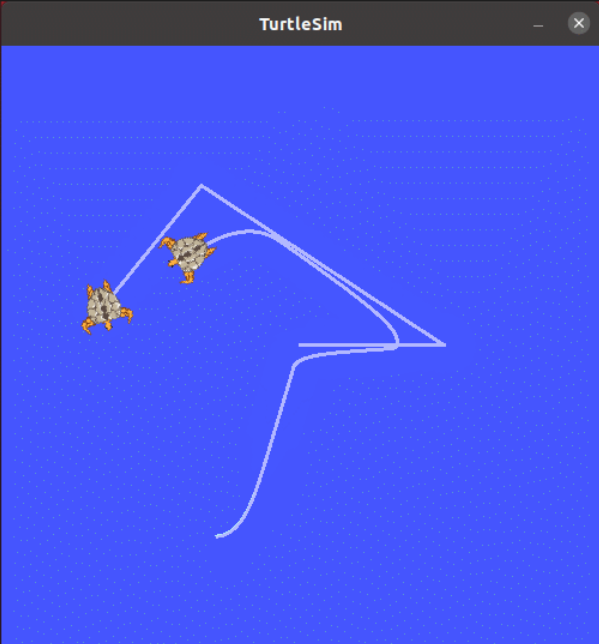
\includegraphics[width=.5\textwidth]{ros_demo_turtle_following.png}
  \caption{乌龟跟随案例演示}
  \label{fig:ros_demo_turtle_following}
\end{figure}

\section{TF坐标变换}

机器人系统上, 有多个传感器, 如激光雷达、摄像头等, 有的传感器是可以感知机器人周边的物体方位 (或者称之为: 坐标, 横向、纵向、高度的距离信息) 的, 以协助机器人定位障碍物, 可以直接将物体相对该传感器的方位信息, 等价于物体相对于机器人系统或机器人其它组件的方位信息吗? 显示是不行的, 这中间需要一个转换过程. 更具体描述如下:

场景1: 雷达与小车

现有一移动式机器人底盘, 在底盘上安装了一雷达, 雷达相对于底盘的偏移量已知, 现雷达检测到一障碍物信息, 获取到坐标分别为 $(x,y,z)$, 该坐标是以雷达为参考系的, 如何将这个坐标转换成以小车为参考系的坐标呢? 

\begin{figure}[!ht]
  \centering
  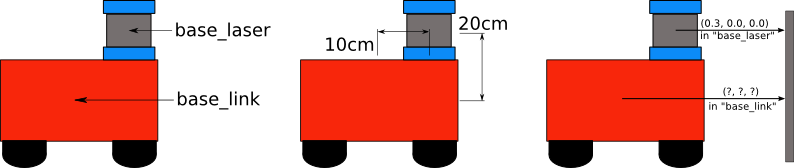
\includegraphics[width=.8\textwidth]{ros_demo_laser_link_01.png}
  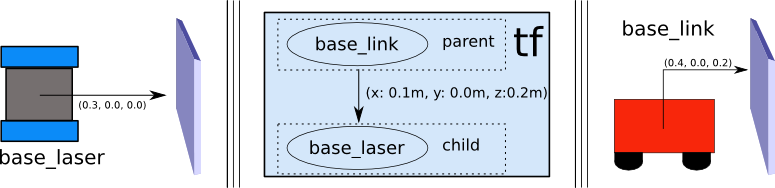
\includegraphics[width=.8\textwidth]{ros_demo_laser_link_02.png}
  \caption{雷达与小车案例演示}
  \label{fig:ros_demo_laser_link}
\end{figure}

场景2: 现有一带机械臂的机器人 (比如: PR2) 需要夹取目标物, 当前机器人头部摄像头可以探测到目标物的坐标 $(x,y,z)$, 不过该坐标是以摄像头为参考系的, 而实际操作目标物的是机械臂的夹具, 当前我们需要将该坐标转换成相对于机械臂夹具的坐标, 这个过程如何实现? 

\begin{figure}[!ht]
  \centering
  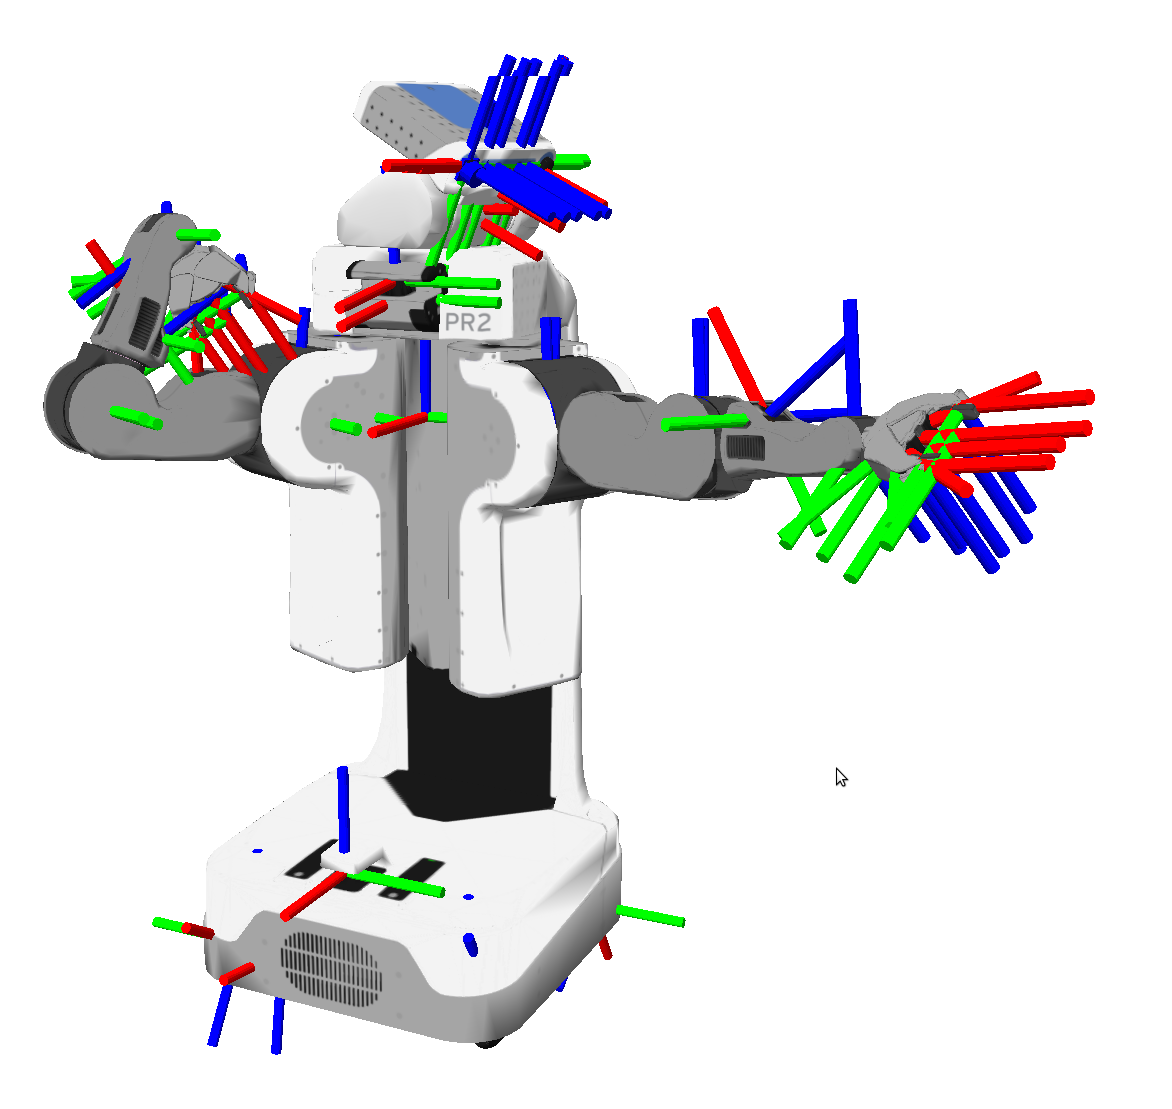
\includegraphics[width=.6\textwidth]{ros_demo_pr2.png}
  \caption{机械臂夹取目标案例演示}
  \label{fig:ros_demo_pr2}
\end{figure}

当然, 根据我们高中学习的知识, 在明确了不同坐标系之间的的相对关系, 就可以实现任何坐标点在不同坐标系之间的转换, 但是该计算实现是较为常用的, 且算法也有点复杂, 因此在 ROS 中直接封装了相关的模块: 坐标变换 (TF).

概念: tf, TransForm Frame, 坐标变换

坐标系: ROS 中是通过坐标系统开标定物体的, 确切的将是通过右手坐标系来标定的.

\begin{figure}[!ht]
  \centering
  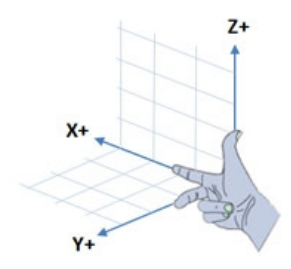
\includegraphics[width=.3\textwidth]{ros_tf_frame.png}
  \caption{TF右手坐标系}
  \label{fig:ros_tf_frame}
\end{figure}

作用: 在 ROS 中用于实现不同坐标系之间的点或向量的转换.

案例: 小乌龟跟随案例: 如本章引言部分演示.

说明: 在 ROS 中坐标变换最初对应的是tf, 不过在 hydro 版本开始, tf 被弃用, 迁移到 tf2, 后者更为简洁高效, tf2对应的常用功能包有:

\begin{itemize}
  \item \verb|tf2_geometry_msgs|: 可以将 ROS 消息转换成tf2消息;
  \item \verb|tf2|: 封装了坐标变换的常用消息;
  \item \verb|tf2_ros|: 为tf2提供了 \verb|roscpp| 和 \verb|rospy| 绑定, 封装了坐标变换常用的API.
\end{itemize}

\subsection{坐标msg消息}

订阅发布模型中数据载体 msg 是一个重要实现, 首先需要了解一下, 在坐标转换实现中常用的 \verb|msg:geometry_msgs/TransformStamped| 和 \verb|geometry_msgs/PointStamped|. 前者用于传输坐标系相关位置信息, 后者用于传输某个坐标系内坐标点的信息. 在坐标变换中, 频繁的需要使用到坐标系的相对关系以及坐标点信息.

1. \verb|geometry_msgs/TransformStamped|

命令行键入:

\begin{bash}
  rosmsg info geometry_msgs/TransformStamped

  std_msgs/Header header                     # 头信息
    uint32 seq                                # |-- 序列号
    time stamp                                # |-- 时间戳
    string frame_id                            # |-- 坐标 ID
  string child_frame_id                    # 子坐标系的 id
  geometry_msgs/Transform transform        # 坐标信息
    geometry_msgs/Vector3 translation        # 偏移量
      float64 x                                # |-- X 方向的偏移量
      float64 y                                # |-- Y 方向的偏移量
      float64 z                                # |-- Z 方向上的偏移量
    geometry_msgs/Quaternion rotation        # 四元数
      float64 x                                
      float64 y                                
      float64 z                                
      float64 w
\end{bash}

四元数用于表示坐标的相对姿态.

2. \verb|geometry_msgs/PointStamped|

命令行键入:

\begin{bash}
  rosmsg info geometry_msgs/PointStamped

  std_msgs/Header header                    # 头
    uint32 seq                                # |-- 序号
    time stamp                                # |-- 时间戳
    string frame_id                            # |-- 所属坐标系的 id
  geometry_msgs/Point point                # 点坐标
    float64 x                                    # |-- x y z 坐标
    float64 y
    float64 z
\end{bash}

\subsection{静态坐标变换}

所谓静态坐标变换, 是指两个坐标系之间的相对位置是固定的.

需求描述: 现有一机器人模型, 核心构成包含主体与雷达, 各对应一坐标系, 坐标系的原点分别位于主体与雷达的物理中心, 已知雷达原点相对于主体原点位移关系如下: $x=0.2$, $y=0.0$, $z=0.5$. 当前雷达检测到一障碍物, 在雷达坐标系中障碍物的坐标为 (2.0 3.0 5.0), 请问, 该障碍物相对于主体的坐标是多少? 

结果演示如图 \ref{fig:ros_demo_static_tf} 所示.

\begin{figure}[!ht]
  \centering
  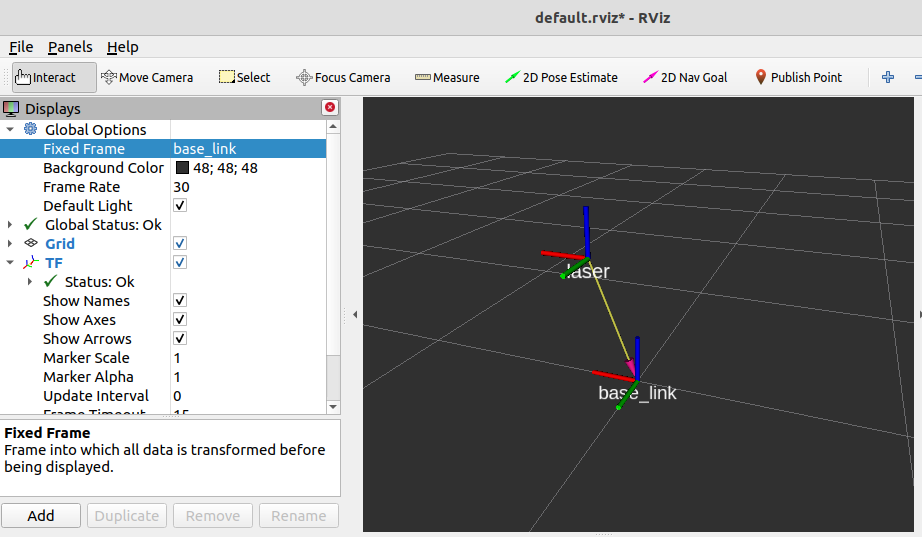
\includegraphics[width=.9\textwidth]{ros_demo_static_tf.png}
  \caption{静态坐标变换结果演示}
  \label{fig:ros_demo_static_tf}
\end{figure}

实现分析:

\begin{itemize}
  \item 坐标系相对关系, 可以通过发布方发布
  \item 订阅方, 订阅到发布的坐标系相对关系, 再传入坐标点信息 (可以写死), 然后借助于 tf 实现坐标变换, 并将结果输出
\end{itemize}

实现流程: C++ 与 Python 实现流程一致

\begin{itemize}
  \item 新建功能包, 添加依赖
  \item 编写发布方实现
  \item 编写订阅方实现
  \item 执行并查看结果
\end{itemize}

方案A: C++实现

1. 创建功能包

创建项目功能包:

\begin{bash}
  catkin_create_pkg your_ros_package tf2 tf2_ros tf2_geometry_msgs roscpp rospy std_msgs geometry_msgs
\end{bash}

2. 发布方

\begin{cpp}
  /* 
      静态坐标变换发布方:
          发布关于 laser 坐标系的位置信息 

      实现流程:
          1. 包含头文件
          2. 初始化 ROS 节点
          3. 创建静态坐标转换广播器
          4. 创建坐标系信息
          5. 广播器发布坐标系信息
          6. spin()
  */

  // 1. 包含头文件
  #include "ros/ros.h"
  #include "tf2_ros/static_transform_broadcaster.h"
  #include "geometry_msgs/TransformStamped.h"
  #include "tf2/LinearMath/Quaternion.h"

  int main(int argc, char *argv[])
  {
      setlocale(LC_ALL,"");
      // 2. 初始化 ROS 节点
      ros::init(argc,argv,"static_brocast");
      // 3. 创建静态坐标转换广播器
      tf2_ros::StaticTransformBroadcaster broadcaster;
      // 4. 创建坐标系信息
      geometry_msgs::TransformStamped ts;
      //----设置头信息
      ts.header.seq = 100;
      ts.header.stamp = ros::Time::now();
      ts.header.frame_id = "base_link";
      //----设置子级坐标系
      ts.child_frame_id = "laser";
      //----设置子级相对于父级的偏移量
      ts.transform.translation.x = 0.2;
      ts.transform.translation.y = 0.0;
      ts.transform.translation.z = 0.5;
      //----设置四元数:将 欧拉角数据转换成四元数
      tf2::Quaternion qtn;
      qtn.setRPY(0,0,0);
      ts.transform.rotation.x = qtn.getX();
      ts.transform.rotation.y = qtn.getY();
      ts.transform.rotation.z = qtn.getZ();
      ts.transform.rotation.w = qtn.getW();
      // 5. 广播器发布坐标系信息
      broadcaster.sendTransform(ts);
      ros::spin();
      return 0;
  }
\end{cpp}

配置文件此处略.

3. 订阅方

\begin{cpp}
  /*  
      订阅坐标系信息, 生成一个相对于 子级坐标系的坐标点数据, 转换成父级坐标系中的坐标点

      实现流程:
          1. 包含头文件
          2. 初始化 ROS 节点
          3. 创建 TF 订阅节点
          4. 生成一个坐标点 (相对于子级坐标系)
          5. 转换坐标点 (相对于父级坐标系)
          6. spin()
  */

  // 1. 包含头文件
  #include "ros/ros.h"
  #include "tf2_ros/transform_listener.h"
  #include "tf2_ros/buffer.h"
  #include "geometry_msgs/PointStamped.h"
  #include "tf2_geometry_msgs/tf2_geometry_msgs.h" // 注意: 调用 transform 必须包含该头文件

  int main(int argc, char *argv[])
  {
      setlocale(LC_ALL,"");
      // 2. 初始化 ROS 节点
      ros::init(argc,argv,"tf_sub");
      ros::NodeHandle nh;
      // 3. 创建 TF 订阅节点
      tf2_ros::Buffer buffer;
      tf2_ros::TransformListener listener(buffer);

      ros::Rate r(1);
      while (ros::ok())
      {
      // 4. 生成一个坐标点 (相对于子级坐标系)
          geometry_msgs::PointStamped point_laser;
          point_laser.header.frame_id = "laser";
          point_laser.header.stamp = ros::Time::now();
          point_laser.point.x = 1;
          point_laser.point.y = 2;
          point_laser.point.z = 7.3;
      // 5. 转换坐标点 (相对于父级坐标系)
          // 新建一个坐标点, 用于接收转换结果  
          //--------------使用 try 语句或休眠, 否则可能由于缓存接收延迟而导致坐标转换失败------------------------
          try
          {
              geometry_msgs::PointStamped point_base;
              point_base = buffer.transform(point_laser,"base_link");
              ROS_INFO("转换后的数据:(%.2f,%.2f,%.2f), 参考的坐标系是:",point_base.point.x,point_base.point.y,point_base.point.z,point_base.header.frame_id.c_str());

          }
          catch(const std::exception& e)
          {
              // std::cerr << e.what() << '\n';
              ROS_INFO("程序异常.....");
          }
          r.sleep();  
          ros::spinOnce();
      }
      return 0;
  }
\end{cpp}

配置文件此处略.

4. 执行

可以使用命令行或launch文件的方式分别启动发布节点与订阅节点, 如果程序无异常, 控制台将输出, 坐标转换后的结果.

方案B: Python实现

1. 创建功能包

创建项目功能包:

\begin{bash}
  catkin_create_pkg your_ros_package tf2 tf2_ros tf2_geometry_msgs roscpp rospy std_msgs geometry_msgs
\end{bash}

2. 发布方

\begin{python}
  #! /usr/bin/env python
  """  
      静态坐标变换发布方:
          发布关于 laser 坐标系的位置信息 
      实现流程:
          1. 导包
          2. 初始化 ROS 节点
          3. 创建 静态坐标广播器
          4. 创建并组织被广播的消息
          5. 广播器发送消息
          6. spin
  """
  # 1. 导包
  import rospy
  import tf2_ros
  import tf
  from geometry_msgs.msg import TransformStamped

  if __name__ == "__main__":
      # 2. 初始化 ROS 节点
      rospy.init_node("static_tf_pub_p")
      # 3. 创建 静态坐标广播器
      broadcaster = tf2_ros.StaticTransformBroadcaster()
      # 4. 创建并组织被广播的消息
      tfs = TransformStamped()
      # --- 头信息
      tfs.header.frame_id = "world"
      tfs.header.stamp = rospy.Time.now()
      tfs.header.seq = 101
      # --- 子坐标系
      tfs.child_frame_id = "radar"
      # --- 坐标系相对信息
      # ------ 偏移量
      tfs.transform.translation.x = 0.2
      tfs.transform.translation.y = 0.0
      tfs.transform.translation.z = 0.5
      # ------ 四元数
      qtn = tf.transformations.quaternion_from_euler(0,0,0)
      tfs.transform.rotation.x = qtn[0]
      tfs.transform.rotation.y = qtn[1]
      tfs.transform.rotation.z = qtn[2]
      tfs.transform.rotation.w = qtn[3]

      # 5. 广播器发送消息
      broadcaster.sendTransform(tfs)
      # 6. spin
      rospy.spin()
\end{python}

权限设置以及配置文件此处略.

3. 订阅方

\begin{python}
  #! /usr/bin/env python
  """  
      订阅坐标系信息, 生成一个相对于 子级坐标系的坐标点数据, 
      转换成父级坐标系中的坐标点

      实现流程:
          1. 导包
          2. 初始化 ROS 节点
          3. 创建 TF 订阅对象
          4. 创建一个 radar 坐标系中的坐标点
          5. 调研订阅对象的 API 将 4 中的点坐标转换成相对于 world 的坐标
          6. spin
  """

  # 1. 导包
  import rospy
  import tf2_ros
  # 不要使用 geometry_msgs, 需要使用 tf2 内置的消息类型
  from tf2_geometry_msgs import PointStamped
  # from geometry_msgs.msg import PointStamped

  if __name__ == "__main__":
      # 2. 初始化 ROS 节点
      rospy.init_node("static_sub_tf_p")
      # 3. 创建 TF 订阅对象
      buffer = tf2_ros.Buffer()
      listener = tf2_ros.TransformListener(buffer)

      rate = rospy.Rate(1)
      while not rospy.is_shutdown():    
      # 4. 创建一个 radar 坐标系中的坐标点
          point_source = PointStamped()
          point_source.header.frame_id = "radar"
          point_source.header.stamp = rospy.Time.now()
          point_source.point.x = 10
          point_source.point.y = 2
          point_source.point.z = 3

          try:
      #     5. 调研订阅对象的 API 将 4 中的点坐标转换成相对于 world 的坐标
              point_target = buffer.transform(point_source,"world")
              rospy.loginfo("转换结果:x = %.2f, y = %.2f, z = %.2f",
                              point_target.point.x,
                              point_target.point.y,
                              point_target.point.z)
          except Exception as e:
              rospy.logerr("异常:%s",e)

      #     6. spin
          rate.sleep()
\end{python}

权限设置以及配置文件此处略.

PS: 在 Python 实现中, tf2 已封装一些消息类型, 不可以使用 \verb|geometry_msgs.msg| 中的类型.

4. 执行

可以使用命令行或 launch 文件的方式分别启动发布节点与订阅节点, 如果程序无异常, 控制台将输出, 坐标转换后的结果.

补充1:

当坐标系之间的相对位置固定时, 那么所需参数也是固定的: 父系坐标名称、子级坐标系名称、$x$ 偏移量、$y$ 偏移量、$z$ 偏移量、$x$ 翻滚角度、$y$ 俯仰角度、$z$ 偏航角度, 实现逻辑相同, 参数不同, 那么 ROS 系统就已经封装好了专门的节点, 使用方式如下:

\begin{bash}
  rosrun tf2_ros static_transform_publisher x偏移量 y偏移量 z偏移量 z偏航角度 y俯仰角度 x翻滚角度 父级坐标系 子级坐标系
\end{bash}

示例:

\begin{bash}
  rosrun tf2_ros static_transform_publisher 0.2 0 0.5 0 0 0 /baselink /laser
\end{bash}

也建议使用该种方式直接实现静态坐标系相对信息发布.

补充2:

可以借助于 RViz 显示坐标系关系, 具体操作:

\begin{itemize}
  \item 新建窗口输入命令: \verb|rviz|;
  \item 在启动的 RViz 中设置 \verb|Fixed Frame| 为 \verb|base_link|;
  \item 点击左下的 \verb|add| 按钮, 在弹出的窗口中选择 TF 组件, 即可显示坐标关系.
\end{itemize}

\subsection{动态坐标变换}

所谓动态坐标变换, 是指两个坐标系之间的相对位置是变化的.

需求描述: 启动 \verb|turtlesim_node|, 该节点中窗体有一个世界坐标系 (左下角为坐标系原点), 乌龟是另一个坐标系, 键盘控制乌龟运动, 将两个坐标系的相对位置动态发布.

结果演示如图 \ref{fig:ros_demo_dynamic_tf} 所示.

\begin{figure}[!ht]
  \centering
  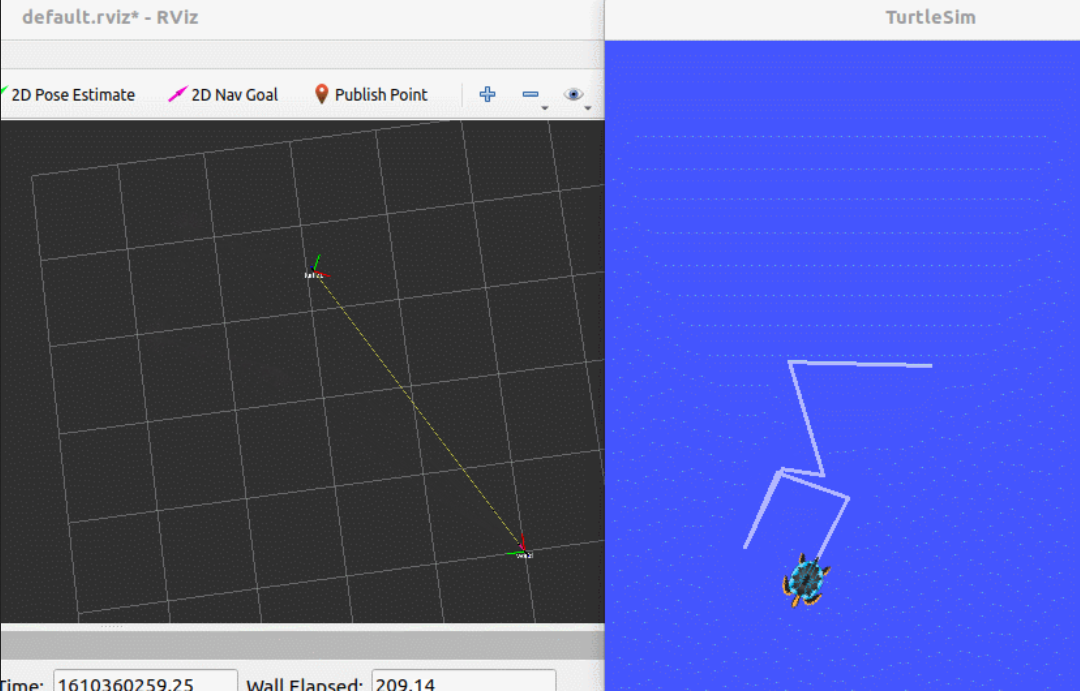
\includegraphics[width=.9\textwidth]{ros_demo_dynamic_tf.png}
  \caption{动态坐标变换结果演示}
  \label{fig:ros_demo_dynamic_tf}
\end{figure}

实现分析:

\begin{itemize}
  \item 乌龟本身不但可以看作坐标系, 也是世界坐标系中的一个坐标点
  \item 订阅 \verb|turtle1/pose|, 可以获取乌龟在世界坐标系的$x$坐标、$y$坐标、偏移量以及线速度和角速度
  \item 将 \verb|pose| 信息转换成 坐标系相对信息并发布
\end{itemize}

实现流程: C++ 与 Python 实现流程一致

\begin{itemize}
  \item 新建功能包, 添加依赖
  \item 创建坐标相对关系发布方 (同时需要订阅乌龟位姿信息)
  \item 创建坐标相对关系订阅方
  \item 执行
\end{itemize}

方案A: C++ 实现

1. 创建功能包

创建项目功能包:

\begin{bash}
  catkin_create_pkg your_ros_package tf2 tf2_ros tf2_geometry_msgs roscpp rospy std_msgs geometry_msgs turtlesim
\end{bash}

2. 发布方

\begin{cpp}
  /*  
      动态的坐标系相对姿态发布 (一个坐标系相对于另一个坐标系的相对姿态是不断变动的)

      需求: 启动 turtlesim_node, 该节点中窗体有一个世界坐标系 (左下角为坐标系原点), 乌龟是另一个坐标系, 键盘
      控制乌龟运动, 将两个坐标系的相对位置动态发布

      实现分析:
          1. 乌龟本身不但可以看作坐标系, 也是世界坐标系中的一个坐标点
          2. 订阅 turtle1/pose, 可以获取乌龟在世界坐标系的 x坐标、y坐标、偏移量以及线速度和角速度
          3. 将 pose 信息转换成 坐标系相对信息并发布

      实现流程:
          1. 包含头文件
          2. 初始化 ROS 节点
          3. 创建 ROS 句柄
          4. 创建订阅对象
          5. 回调函数处理订阅到的数据 (实现TF广播)
              5-1. 创建 TF 广播器
              5-2. 创建 广播的数据 (通过 pose 设置)
              5-3. 广播器发布数据
          6. spin
  */
  // 1. 包含头文件
  #include "ros/ros.h"
  #include "turtlesim/Pose.h"
  #include "tf2_ros/transform_broadcaster.h"
  #include "geometry_msgs/TransformStamped.h"
  #include "tf2/LinearMath/Quaternion.h"

  void doPose(const turtlesim::Pose::ConstPtr& pose){
      //  5-1. 创建 TF 广播器
      static tf2_ros::TransformBroadcaster broadcaster;
      //  5-2. 创建 广播的数据 (通过 pose 设置)
      geometry_msgs::TransformStamped tfs;
      //  |----头设置
      tfs.header.frame_id = "world";
      tfs.header.stamp = ros::Time::now();

      //  |----坐标系 ID
      tfs.child_frame_id = "turtle1";

      //  |----坐标系相对信息设置
      tfs.transform.translation.x = pose->x;
      tfs.transform.translation.y = pose->y;
      tfs.transform.translation.z = 0.0; // 二维实现, pose 中没有z, z 是 0
      //  |--------- 四元数设置
      tf2::Quaternion qtn;
      qtn.setRPY(0,0,pose->theta);
      tfs.transform.rotation.x = qtn.getX();
      tfs.transform.rotation.y = qtn.getY();
      tfs.transform.rotation.z = qtn.getZ();
      tfs.transform.rotation.w = qtn.getW();

      //  5-3. 广播器发布数据
      broadcaster.sendTransform(tfs);
  }

  int main(int argc, char *argv[])
  {
      setlocale(LC_ALL,"");
      // 2. 初始化 ROS 节点
      ros::init(argc,argv,"dynamic_tf_pub");
      // 3. 创建 ROS 句柄
      ros::NodeHandle nh;
      // 4. 创建订阅对象
      ros::Subscriber sub = nh.subscribe<turtlesim::Pose>("/turtle1/pose",1000,doPose);
      //     5. 回调函数处理订阅到的数据 (实现TF广播)
      //        
      // 6. spin
      ros::spin();
      return 0;
  }
\end{cpp}

配置文件此处略.

3. 订阅方

\begin{cpp}
  // 1. 包含头文件
  #include "ros/ros.h"
  #include "tf2_ros/transform_listener.h"
  #include "tf2_ros/buffer.h"
  #include "geometry_msgs/PointStamped.h"
  #include "tf2_geometry_msgs/tf2_geometry_msgs.h" // 注意: 调用 transform 必须包含该头文件

  int main(int argc, char *argv[])
  {
      setlocale(LC_ALL,"");
      // 2. 初始化 ROS 节点
      ros::init(argc,argv,"dynamic_tf_sub");
      ros::NodeHandle nh;
      // 3. 创建 TF 订阅节点
      tf2_ros::Buffer buffer;
      tf2_ros::TransformListener listener(buffer);

      ros::Rate r(1);
      while (ros::ok())
      {
      // 4. 生成一个坐标点 (相对于子级坐标系)
          geometry_msgs::PointStamped point_laser;
          point_laser.header.frame_id = "turtle1";
          point_laser.header.stamp = ros::Time();
          point_laser.point.x = 1;
          point_laser.point.y = 1;
          point_laser.point.z = 0;
      // 5. 转换坐标点 (相对于父级坐标系)
          // 新建一个坐标点, 用于接收转换结果  
          //--------------使用 try 语句或休眠, 否则可能由于缓存接收延迟而导致坐标转换失败------------------------
          try
          {
              geometry_msgs::PointStamped point_base;
              point_base = buffer.transform(point_laser,"world");
              ROS_INFO("坐标点相对于 world 的坐标为:(%.2f,%.2f,%.2f)",point_base.point.x,point_base.point.y,point_base.point.z);

          }
          catch(const std::exception& e)
          {
              // std::cerr << e.what() << '\n';
              ROS_INFO("程序异常:%s",e.what());
          }

          r.sleep();  
          ros::spinOnce();
      }

      return 0;
  }
\end{cpp}

配置文件此处略.

4. 执行

可以使用命令行或 launch 文件的方式分别启动发布节点与订阅节点, 如果程序无异常, 与演示结果类似.

可以使用 RViz 查看坐标系相对关系.

方案B: Python 实现

1. 创建功能包

创建项目功能包:

\begin{bash}
  catkin_create_pkg your_ros_package tf2 tf2_ros tf2_geometry_msgs roscpp rospy std_msgs geometry_msgs turtlesim
\end{bash}

2. 发布方

\begin{python}
  #! /usr/bin/env python
  """  
      动态的坐标系相对姿态发布 (一个坐标系相对于另一个坐标系的相对姿态是不断变动的)

      需求: 启动 turtlesim_node, 该节点中窗体有一个世界坐标系 (左下角为坐标系原点), 乌龟是另一个坐标系, 键盘
      控制乌龟运动, 将两个坐标系的相对位置动态发布

      实现分析:
          1. 乌龟本身不但可以看作坐标系, 也是世界坐标系中的一个坐标点
          2. 订阅 turtle1/pose, 可以获取乌龟在世界坐标系的 x坐标、y坐标、偏移量以及线速度和角速度
          3. 将 pose 信息转换成 坐标系相对信息并发布
      实现流程:
          1. 导包
          2. 初始化 ROS 节点
          3. 订阅 /turtle1/pose 话题消息
          4. 回调函数处理
              4-1. 创建 TF 广播器
              4-2. 创建 广播的数据 (通过 pose 设置)
              4-3. 广播器发布数据
          5. spin
  """

  # 1. 导包
  import rospy
  import tf2_ros
  import tf
  from turtlesim.msg import Pose
  from geometry_msgs.msg import TransformStamped

  #     4. 回调函数处理
  def doPose(pose):
      #         4-1. 创建 TF 广播器
      broadcaster = tf2_ros.TransformBroadcaster()
      #         4-2. 创建 广播的数据 (通过 pose 设置)
      tfs = TransformStamped()
      tfs.header.frame_id = "world"
      tfs.header.stamp = rospy.Time.now()
      tfs.child_frame_id = "turtle1"
      tfs.transform.translation.x = pose.x
      tfs.transform.translation.y = pose.y
      tfs.transform.translation.z = 0.0
      qtn = tf.transformations.quaternion_from_euler(0,0,pose.theta)
      tfs.transform.rotation.x = qtn[0]
      tfs.transform.rotation.y = qtn[1]
      tfs.transform.rotation.z = qtn[2]
      tfs.transform.rotation.w = qtn[3]
      #         4-3. 广播器发布数据
      broadcaster.sendTransform(tfs)

  if __name__ == "__main__":
      # 2. 初始化 ROS 节点
      rospy.init_node("dynamic_tf_pub_p")
      # 3. 订阅 /turtle1/pose 话题消息
      sub = rospy.Subscriber("/turtle1/pose",Pose,doPose)
      #     4. 回调函数处理
      #         4-1. 创建 TF 广播器
      #         4-2. 创建 广播的数据 (通过 pose 设置)
      #         4-3. 广播器发布数据
      #     5. spin
      rospy.spin()
\end{python}

权限设置以及配置文件此处略.

3. 订阅方

\begin{python}
  #! /usr/bin/env python
  """  
      动态的坐标系相对姿态发布 (一个坐标系相对于另一个坐标系的相对姿态是不断变动的)

      需求: 启动 turtlesim_node, 该节点中窗体有一个世界坐标系 (左下角为坐标系原点), 乌龟是另一个坐标系, 键盘
      控制乌龟运动, 将两个坐标系的相对位置动态发布

      实现分析:
          1. 乌龟本身不但可以看作坐标系, 也是世界坐标系中的一个坐标点
          2. 订阅 turtle1/pose, 可以获取乌龟在世界坐标系的 x坐标、y坐标、偏移量以及线速度和角速度
          3. 将 pose 信息转换成 坐标系相对信息并发布
      实现流程:
          1. 导包
          2. 初始化 ROS 节点
          3. 创建 TF 订阅对象
          4. 处理订阅的数据


  """
  # 1. 导包
  import rospy
  import tf2_ros
  # 不要使用 geometry_msgs, 需要使用 tf2 内置的消息类型
  from tf2_geometry_msgs import PointStamped
  # from geometry_msgs.msg import PointStamped

  if __name__ == "__main__":
      # 2. 初始化 ROS 节点
      rospy.init_node("static_sub_tf_p")
      # 3. 创建 TF 订阅对象
      buffer = tf2_ros.Buffer()
      listener = tf2_ros.TransformListener(buffer)

      rate = rospy.Rate(1)
      while not rospy.is_shutdown():    
      # 4. 创建一个 radar 坐标系中的坐标点
          point_source = PointStamped()
          point_source.header.frame_id = "turtle1"
          point_source.header.stamp = rospy.Time.now()
          point_source.point.x = 10
          point_source.point.y = 2
          point_source.point.z = 3

          try:
      #     5. 调研订阅对象的 API 将 4 中的点坐标转换成相对于 world 的坐标
              point_target = buffer.transform(point_source,"world",rospy.Duration(1))
              rospy.loginfo("转换结果:x = %.2f, y = %.2f, z = %.2f",
                              point_target.point.x,
                              point_target.point.y,
                              point_target.point.z)
          except Exception as e:
              rospy.logerr("异常:%s",e)

      #     6. spin
          rate.sleep()
\end{python}

权限设置以及配置文件此处略.

4. 执行

可以使用命令行或 launch 文件的方式分别启动发布节点与订阅节点, 如果程序无异常, 与演示结果类似.

可以使用 RViz 查看坐标系相对关系.

\subsection{多坐标变换}

需求描述: 现有坐标系统, 父级坐标系统 world, 下有两子级系统 son1, son2, son1 相对于 world, 以及 son2 相对于 world 的关系是已知的, 求 son1 原点在 son2 中的坐标, 又已知在 son1 中一点的坐标, 要求求出该点在 son2 中的坐标.

实现分析:

\begin{itemize}
  \item 首先, 需要发布 son1 相对于 world, 以及 son2 相对于 world 的坐标消息;
  \item 然后, 需要订阅坐标发布消息, 并取出订阅的消息, 借助于 tf2 实现 son1 和 son2 的转换;
  \item 最后, 还要实现坐标点的转换.
\end{itemize}

实现流程: C++ 与 Python 实现流程一致

\begin{itemize}
  \item 新建功能包, 添加依赖;
  \item 创建坐标相对关系发布方 (需要发布两个坐标相对关系);
  \item 创建坐标相对关系订阅方;
  \item 执行.
\end{itemize}

方案A: C++ 实现

1. 创建功能包

创建项目功能包:

\begin{bash}
  catkin_create_pkg your_ros_package tf2 tf2_ros tf2_geometry_msgs roscpp rospy std_msgs geometry_msgs turtlesim
\end{bash}

2. 发布方

为了方便, 使用静态坐标变换发布.

\begin{xml}
  <launch>
      <node pkg="tf2_ros" type="static_transform_publisher" name="son1" args="0.2 0.8 0.3 0 0 0 /world /son1" output="screen" />
      <node pkg="tf2_ros" type="static_transform_publisher" name="son2" args="0.5 0 0 0 0 0 /world /son2" output="screen" />
  </launch>
\end{xml}

3. 订阅方

\begin{cpp}
  /*
  需求:
      现有坐标系统, 父级坐标系统 world, 下有两子级系统 son1, son2, 
      son1 相对于 world, 以及 son2 相对于 world 的关系是已知的, 
      求 son1 与 son2 中的坐标关系, 又已知在 son1 中一点的坐标, 要求求出该点在 son2 中的坐标
  实现流程:
      1. 包含头文件
      2. 初始化 ROS 节点
      3. 创建 ROS 句柄
      4. 创建 TF 订阅对象
      5. 解析订阅信息中获取 son1 坐标系原点在 son2 中的坐标
        解析 son1 中的点相对于 son2 的坐标
      6. spin
  */

  // 1. 包含头文件
  #include "ros/ros.h"
  #include "tf2_ros/transform_listener.h"
  #include "tf2/LinearMath/Quaternion.h"
  #include "tf2_geometry_msgs/tf2_geometry_msgs.h"
  #include "geometry_msgs/TransformStamped.h"
  #include "geometry_msgs/PointStamped.h"

  int main(int argc, char *argv[])
  {   setlocale(LC_ALL,"");
      // 2. 初始化 ROS 节点
      ros::init(argc,argv,"sub_frames");
      // 3. 创建 ROS 句柄
      ros::NodeHandle nh;
      // 4. 创建 TF 订阅对象
      tf2_ros::Buffer buffer; 
      tf2_ros::TransformListener listener(buffer);
      // 5. 解析订阅信息中获取 son1 坐标系原点在 son2 中的坐标
      ros::Rate r(1);
      while (ros::ok())
      {
          try
          {
          //   解析 son1 中的点相对于 son2 的坐标
              geometry_msgs::TransformStamped tfs = buffer.lookupTransform("son2","son1",ros::Time(0));
              ROS_INFO("Son1 相对于 Son2 的坐标关系:父坐标系ID=%s",tfs.header.frame_id.c_str());
              ROS_INFO("Son1 相对于 Son2 的坐标关系:子坐标系ID=%s",tfs.child_frame_id.c_str());
              ROS_INFO("Son1 相对于 Son2 的坐标关系:x=%.2f,y=%.2f,z=%.2f",
                      tfs.transform.translation.x,
                      tfs.transform.translation.y,
                      tfs.transform.translation.z
                      );

              // 坐标点解析
              geometry_msgs::PointStamped ps;
              ps.header.frame_id = "son1";
              ps.header.stamp = ros::Time::now();
              ps.point.x = 1.0;
              ps.point.y = 2.0;
              ps.point.z = 3.0;

              geometry_msgs::PointStamped psAtSon2;
              psAtSon2 = buffer.transform(ps,"son2");
              ROS_INFO("在 Son2 中的坐标:x=%.2f,y=%.2f,z=%.2f",
                      psAtSon2.point.x,
                      psAtSon2.point.y,
                      psAtSon2.point.z
                      );
          }
          catch(const std::exception& e)
          {
              // std::cerr << e.what() << '\n';
              ROS_INFO("异常信息:%s",e.what());
          }

          r.sleep();
          // 6. spin
          ros::spinOnce();
      }
      return 0;
  }
\end{cpp}

配置文件此处略.

4. 执行

可以使用命令行或 launch 文件的方式分别启动发布节点与订阅节点, 如果程序无异常, 将输出换算后的结果.

方案B: Python 实现

1. 创建功能包

创建项目功能包:

\begin{bash}
  catkin_create_pkg your_ros_package tf2 tf2_ros tf2_geometry_msgs roscpp rospy std_msgs geometry_msgs turtlesim
\end{bash}

2. 发布方

为了方便, 使用静态坐标变换发布.

\begin{xml}
  <launch>
      <node pkg="tf2_ros" type="static_transform_publisher" name="son1" args="0.2 0.8 0.3 0 0 0 /world /son1" output="screen" />
      <node pkg="tf2_ros" type="static_transform_publisher" name="son2" args="0.5 0 0 0 0 0 /world /son2" output="screen" />
  </launch>
\end{xml}

3. 订阅方

\begin{python}
  #!/usr/bin/env python
  """  
      需求:
          现有坐标系统, 父级坐标系统 world, 下有两子级系统 son1, son2, 
          son1 相对于 world, 以及 son2 相对于 world 的关系是已知的, 
          求 son1 与 son2中的坐标关系, 又已知在 son1中一点的坐标, 要求求出该点在 son2 中的坐标
      实现流程:   
          1. 导包
          2. 初始化 ROS 节点
          3. 创建 TF 订阅对象
          4. 调用 API 求出 son1 相对于 son2 的坐标关系
          5. 创建一依赖于 son1 的坐标点, 调用 API 求出该点在 son2 中的坐标
          6. spin
  """

  # 1. 导包
  import rospy
  import tf2_ros
  from geometry_msgs.msg import TransformStamped
  from tf2_geometry_msgs import PointStamped

  if __name__ == "__main__":

      # 2. 初始化 ROS 节点
      rospy.init_node("frames_sub_p")
      # 3. 创建 TF 订阅对象
      buffer = tf2_ros.Buffer()
      listener = tf2_ros.TransformListener(buffer)

      rate = rospy.Rate(1)
      while not rospy.is_shutdown():

          try:
          # 4. 调用 API 求出 son1 相对于 son2 的坐标关系
              # lookup_transform(self, target_frame, source_frame, time, timeout=rospy.Duration(0.0)):
              tfs = buffer.lookup_transform("son2","son1",rospy.Time(0))
              rospy.loginfo("son1 与 son2 相对关系:")
              rospy.loginfo("父级坐标系:%s",tfs.header.frame_id)
              rospy.loginfo("子级坐标系:%s",tfs.child_frame_id)
              rospy.loginfo("相对坐标:x=%.2f, y=%.2f, z=%.2f",
                          tfs.transform.translation.x,
                          tfs.transform.translation.y,
                          tfs.transform.translation.z,
              )
          # 5. 创建一依赖于 son1 的坐标点, 调用 API 求出该点在 son2 中的坐标
              point_source = PointStamped()
              point_source.header.frame_id = "son1"
              point_source.header.stamp = rospy.Time.now()
              point_source.point.x = 1
              point_source.point.y = 1
              point_source.point.z = 1

              point_target = buffer.transform(point_source,"son2",rospy.Duration(0.5))

              rospy.loginfo("point_target 所属的坐标系:%s",point_target.header.frame_id)
              rospy.loginfo("坐标点相对于 son2 的坐标:(%.2f,%.2f,%.2f)",
                          point_target.point.x,
                          point_target.point.y,
                          point_target.point.z
              )

          except Exception as e:
              rospy.logerr("错误提示:%s",e)

          rate.sleep()
      # 6. spin    
      # rospy.spin()
\end{python}

权限设置以及配置文件此处略.

4. 执行

可以使用命令行或 launch 文件的方式分别启动发布节点与订阅节点, 如果程序无异常, 将输出换算后的结果.

\subsection{坐标系关系查看}

在机器人系统中, 涉及的坐标系有多个, 为了方便查看, ROS 提供了专门的工具, 可以用于生成显示坐标系关系的 PDF 文件, 该文件包含树形结构的坐标系图谱.

1. 准备

首先调用 \verb|rospack find tf2_tools| 查看是否包含该功能包, 如果没有, 请使用如下命令安装:

\begin{bash}
  sudo apt install ros-noetic-tf2-tools
\end{bash}

2. 使用

生成 PDF 文件: 启动坐标系广播程序之后, 运行如下命令:

\begin{bash}
  rosrun tf2_tools view_frames.py
\end{bash}

会产生类似于下面的日志信息:

\begin{bash}
  [INFO] [1592920556.827549]: Listening to tf data during 5 seconds...
  [INFO] [1592920561.841536]: Generating graph in frames.pdf file...
\end{bash}

查看当前目录会生成一个 \verb|frames.pdf| 文件

查看文件: 可以直接进入目录打开文件, 或者调用命令查看文件:

\begin{bash}
  evince frames.pdf
\end{bash}

内容如图 \ref{fig:ros_demo_frame_pdf} 所示.

\begin{figure}[!ht]
  \centering
  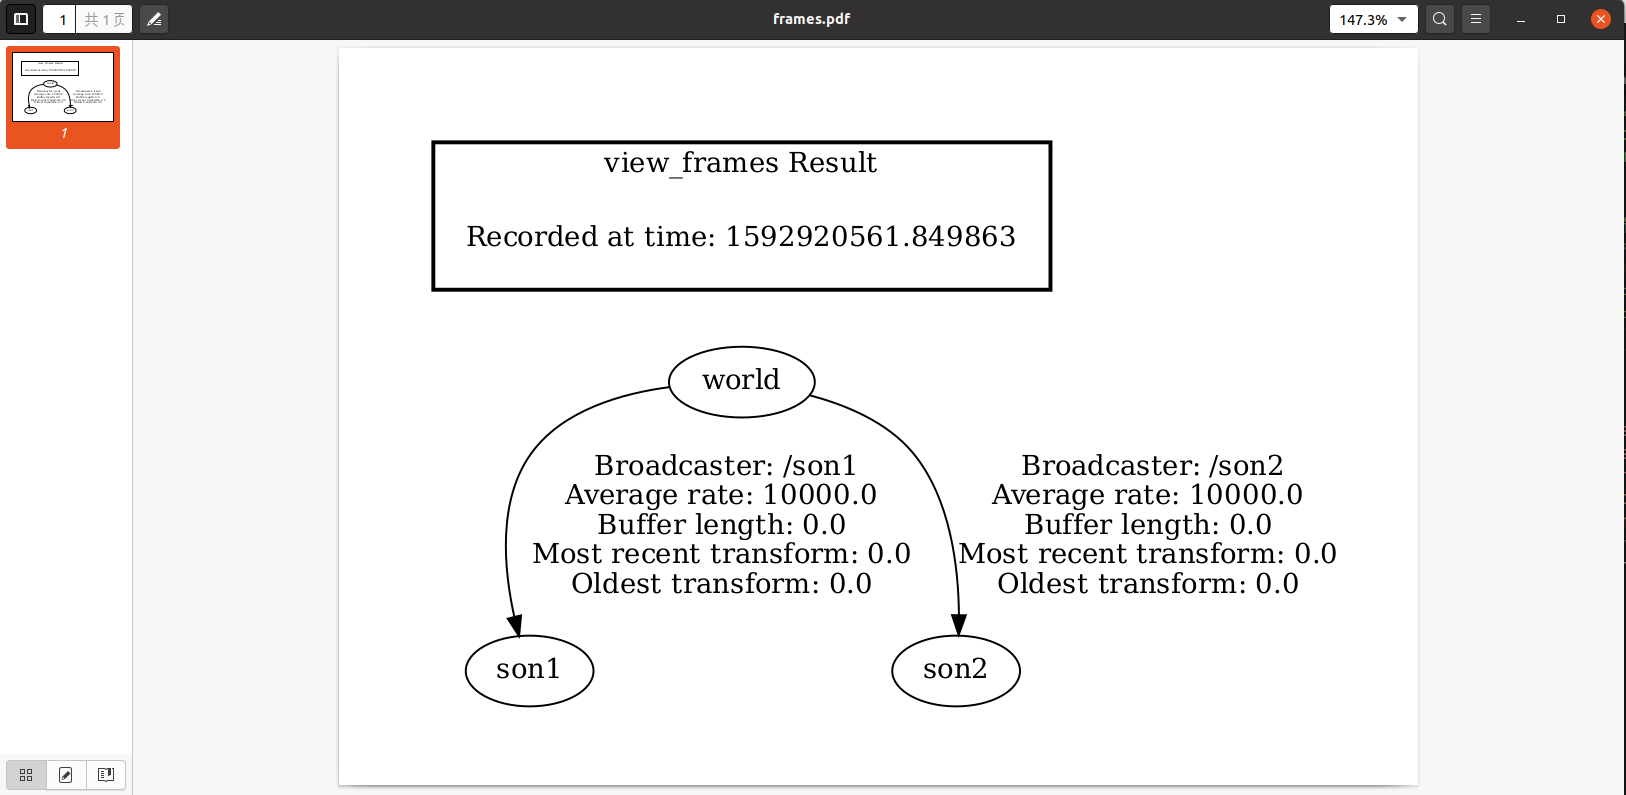
\includegraphics[width=.9\textwidth]{ros_demo_frame_pdf.png}
  \caption{坐标系关系查看结果演示}
  \label{fig:ros_demo_frame_pdf}
\end{figure}

\subsection{TF坐标变换实操}

需求描述: 程序启动之初产生两只乌龟, 中间的乌龟 (A) 和 左下乌龟 (B), B 会自动运行至 A 的位置, 并且键盘控制时, 只是控制 A 的运动, 但是 B 可以跟随 A 运行.

结果演示如图 \ref{fig:ros_demo_turtle_following_02} 所示.

\begin{figure}[!ht]
  \centering
  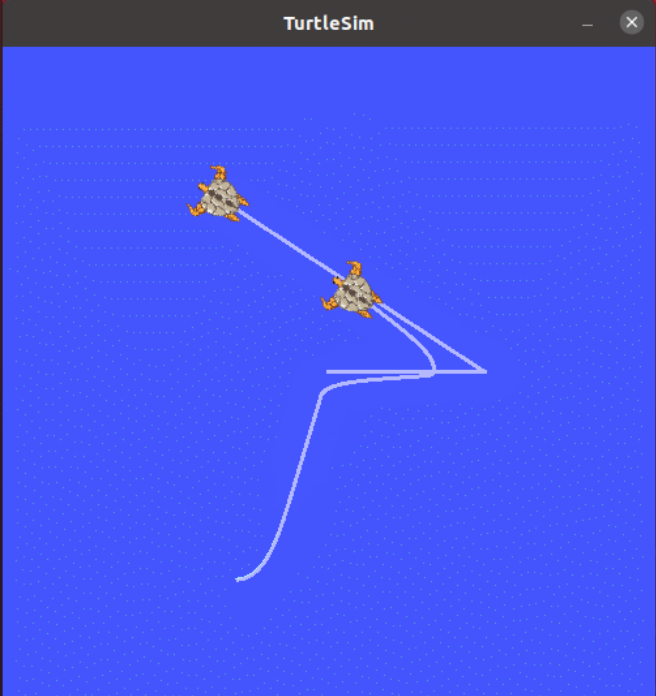
\includegraphics[width=.5\textwidth]{ros_demo_turtle_following_02.png}
  \caption{TF坐标变换结果演示}
  \label{fig:ros_demo_turtle_following_02}
\end{figure}

实现分析: 乌龟跟随实现的核心, 是乌龟 A 和 B 都要发布相对世界坐标系的坐标信息, 然后, 订阅到该信息需要转换获取 A 相对于 B 坐标系的信息, 最后, 再生成速度信息, 并控制 B 运动.

\begin{itemize}
  \item 启动乌龟显示节点;
  \item 在乌龟显示窗体中生成一只新的乌龟 (需要使用服务);
  \item 编写两只乌龟发布坐标信息的节点;
  \item 编写订阅节点订阅坐标信息并生成新的相对关系生成速度信息.
\end{itemize}

实现流程: C++ 与 Python 实现流程一致:

\begin{itemize}
  \item 新建功能包, 添加依赖;
  \item 编写服务客户端, 用于生成一只新的乌龟;
  \item 编写发布方, 发布两只乌龟的坐标信息;
  \item 编写订阅方, 订阅两只乌龟信息, 生成速度信息并发布;
  \item 运行.
\end{itemize}

准备工作:

1. 了解如何创建第二只乌龟, 且不受键盘控制

创建第二只乌龟需要使用 \verb|rosservice|, 话题使用的是 \verb|spawn|:

\begin{bash}
  rosservice call /spawn "x: 1.0
  y: 1.0
  theta: 1.0
  name: 'turtle_flow'" 
  name: "turtle_flow"
\end{bash}

键盘是无法控制第二只乌龟运动的, 因为使用的话题: \verb|/第二只乌龟名称/cmd_vel|, 对应的要控制乌龟运动必须发布对应的话题消息.

2. 了解如何获取两只乌龟的坐标

通过话题 \verb|/乌龟名称/pose| 获取:

\begin{bash}
  x: 1.0                  # x坐标
  y: 1.0                  # y坐标
  theta: -1.21437060833   # 角度
  linear_velocity: 0.0    # 线速度
  angular_velocity: 1.0   # 角速度
\end{bash}

方案A: C++ 实现

1. 创建功能包

创建项目功能包:

\begin{bash}
  catkin_create_pkg your_ros_package tf2 tf2_ros tf2_geometry_msgs roscpp rospy std_msgs geometry_msgs turtlesim
\end{bash}

2. 服务客户端 (生成乌龟)

\begin{cpp}
  /* 
   *  创建第二只小乌龟
   */

  #include "ros/ros.h"
  #include "turtlesim/Spawn.h"

  int main(int argc, char *argv[])
  {
      setlocale(LC_ALL,"");

      // 执行初始化
      ros::init(argc,argv,"create_turtle");
      // 创建节点
      ros::NodeHandle nh;
      // 创建服务客户端
      ros::ServiceClient client = nh.serviceClient<turtlesim::Spawn>("/spawn");

      ros::service::waitForService("/spawn");
      turtlesim::Spawn spawn;
      spawn.request.name = "turtle2";
      spawn.request.x = 1.0;
      spawn.request.y = 2.0;
      spawn.request.theta = 3.12415926;
      bool flag = client.call(spawn);
      if (flag)
      {
          ROS_INFO("乌龟%s创建成功!",spawn.response.name.c_str());
      }
      else
      {
          ROS_INFO("乌龟2创建失败!");
      }

      ros::spin();

      return 0;
  }
\end{cpp}

配置文件此处略.

3. 发布方 (发布两只乌龟的坐标信息)

可以订阅乌龟的位姿信息, 然后再转换成坐标信息, 两只乌龟的实现逻辑相同, 只是订阅的话题名称, 生成的坐标信息等稍有差异, 可以将差异部分通过参数传入: 该节点需要启动两次; 每次启动时都需要传入乌龟节点名称 (第一次是 turtle1 第二次是 turtle2).

\begin{cpp}
  /*  
      该文件实现:需要订阅 turtle1 和 turtle2 的 pose, 然后广播相对 world 的坐标系信息

      注意: 订阅的两只 turtle, 除了命名空间 (turtle1 和 turtle2) 不同外,
            其他的话题名称和实现逻辑都是一样的, 
            所以我们可以将所需的命名空间通过 args 动态传入

      实现流程:
          1. 包含头文件
          2. 初始化 ROS 节点
          3. 解析传入的命名空间
          4. 创建 ROS 句柄
          5. 创建订阅对象
          6. 回调函数处理订阅的 pose 信息
              6-1. 创建 TF 广播器
              6-2. 将 pose 信息转换成 TransFormStamped
              6-3. 发布
          7. spin
  */

  // 1. 包含头文件
  #include "ros/ros.h"
  #include "turtlesim/Pose.h"
  #include "tf2_ros/transform_broadcaster.h"
  #include "tf2/LinearMath/Quaternion.h"
  #include "geometry_msgs/TransformStamped.h"
  // 保存乌龟名称
  std::string turtle_name;

  void doPose(const turtlesim::Pose::ConstPtr& pose){
      //  6-1. 创建 TF 广播器 ---------------------------------------- 注意 static
      static tf2_ros::TransformBroadcaster broadcaster;
      //  6-2. 将 pose 信息转换成 TransFormStamped
      geometry_msgs::TransformStamped tfs;
      tfs.header.frame_id = "world";
      tfs.header.stamp = ros::Time::now();
      tfs.child_frame_id = turtle_name;
      tfs.transform.translation.x = pose->x;
      tfs.transform.translation.y = pose->y;
      tfs.transform.translation.z = 0.0;
      tf2::Quaternion qtn;
      qtn.setRPY(0,0,pose->theta);
      tfs.transform.rotation.x = qtn.getX();
      tfs.transform.rotation.y = qtn.getY();
      tfs.transform.rotation.z = qtn.getZ();
      tfs.transform.rotation.w = qtn.getW();
      //  6-3. 发布
      broadcaster.sendTransform(tfs);
  } 

  int main(int argc, char *argv[])
  {
      setlocale(LC_ALL,"");
      // 2. 初始化 ROS 节点
      ros::init(argc,argv,"pub_tf");
      // 3. 解析传入的命名空间
      if (argc != 2)
      {
          ROS_ERROR("请传入正确的参数");
      } else {
          turtle_name = argv[1];
          ROS_INFO("乌龟 %s 坐标发送启动",turtle_name.c_str());
      }

      // 4. 创建 ROS 句柄
      ros::NodeHandle nh;
      // 5. 创建订阅对象
      ros::Subscriber sub = nh.subscribe<turtlesim::Pose>(turtle_name + "/pose",1000,doPose);
      //     6. 回调函数处理订阅的 pose 信息
      //         6-1. 创建 TF 广播器
      //         6-2. 将 pose 信息转换成 TransFormStamped
      //         6-3. 发布
      // 7. spin
      ros::spin();
      return 0;
  }
\end{cpp}

配置文件此处略.

4. 订阅方 (解析坐标信息并生成速度信息)

\begin{cpp}
  /*  
      订阅 turtle1 和 turtle2 的 TF 广播信息, 查找并转换时间最近的 TF 信息
      将 turtle1 转换成相对 turtle2 的坐标, 在计算线速度和角速度并发布

      实现流程:
          1. 包含头文件
          2. 初始化 ROS 节点
          3. 创建 ROS 句柄
          4. 创建 TF 订阅对象
          5. 处理订阅到的 TF
          6. spin
  */

  // 1. 包含头文件
  #include "ros/ros.h"
  #include "tf2_ros/transform_listener.h"
  #include "geometry_msgs/TransformStamped.h"
  #include "geometry_msgs/Twist.h"

  int main(int argc, char *argv[])
  {
      setlocale(LC_ALL,"");
      // 2. 初始化 ROS 节点
      ros::init(argc,argv,"sub_TF");
      // 3. 创建 ROS 句柄
      ros::NodeHandle nh;
      // 4. 创建 TF 订阅对象
      tf2_ros::Buffer buffer;
      tf2_ros::TransformListener listener(buffer);
      // 5. 处理订阅到的 TF

      // 需要创建发布 /turtle2/cmd_vel 的 publisher 对象

      ros::Publisher pub = nh.advertise<geometry_msgs::Twist>("/turtle2/cmd_vel",1000);

      ros::Rate rate(10);
      while (ros::ok())
      {
          try
          {
              // 5-1. 先获取 turtle1 相对 turtle2 的坐标信息
              geometry_msgs::TransformStamped tfs = buffer.lookupTransform("turtle2","turtle1",ros::Time(0));

              // 5-2. 根据坐标信息生成速度信息 -- geometry_msgs/Twist.h
              geometry_msgs::Twist twist;
              twist.linear.x = 0.5 * sqrt(pow(tfs.transform.translation.x,2) + pow(tfs.transform.translation.y,2));
              twist.angular.z = 4 * atan2(tfs.transform.translation.y,tfs.transform.translation.x);

              // 5-3. 发布速度信息 -- 需要提前创建 publish 对象
              pub.publish(twist);
          }
          catch(const std::exception& e)
          {
              // std::cerr << e.what() << '\n';
              ROS_INFO("错误提示:%s",e.what());
          }
          rate.sleep();
          // 6. spin
          ros::spinOnce();
      }
      return 0;
  }
\end{cpp}

配置文件此处略.

5. 运行

使用 launch 文件组织需要运行的节点, 内容示例如下:

\begin{xml}
  <!-- tf2 实现小乌龟跟随案例 -->
  <launch>
      <!-- 启动乌龟节点与键盘控制节点 -->
      <node pkg="turtlesim" type="turtlesim_node" name="turtle1" output="screen" />
      <node pkg="turtlesim" type="turtle_teleop_key" name="key_control" output="screen"/>
      <!-- 启动创建第二只乌龟的节点 -->
      <node pkg="demo_tf2_test" type="Test01_Create_Turtle2" name="turtle2" output="screen" />
      <!-- 启动两个坐标发布节点 -->
      <node pkg="demo_tf2_test" type="Test02_TF2_Caster" name="caster1" output="screen" args="turtle1" />
      <node pkg="demo_tf2_test" type="Test02_TF2_Caster" name="caster2" output="screen" args="turtle2" />
      <!-- 启动坐标转换节点 -->
      <node pkg="demo_tf2_test" type="Test03_TF2_Listener" name="listener" output="screen" />
  </launch>
\end{xml}

方案B: Python实现

1. 创建功能包

创建项目功能包:

\begin{bash}
  catkin_create_pkg your_ros_package tf2 tf2_ros tf2_geometry_msgs roscpp rospy std_msgs geometry_msgs turtlesim
\end{bash}

2. 服务客户端 (生成乌龟)

\begin{python}
  #! /usr/bin/env python
  """  
      调用 service 服务在窗体指定位置生成一只乌龟
      流程:
          1. 导包
          2. 初始化 ROS 节点
          3. 创建服务客户端
          4. 等待服务启动
          5. 创建请求数据
          6. 发送请求并处理响应
  """

  # 1. 导包
  import rospy
  from turtlesim.srv import Spawn, SpawnRequest, SpawnResponse

  if __name__ == "__main__":
      # 2. 初始化 ROS 节点
      rospy.init_node("turtle_spawn_p")
      # 3. 创建服务客户端
      client = rospy.ServiceProxy("/spawn",Spawn)
      # 4. 等待服务启动
      client.wait_for_service()
      # 5. 创建请求数据
      req = SpawnRequest()
      req.x = 1.0
      req.y = 1.0
      req.theta = 3.14
      req.name = "turtle2"
      # 6. 发送请求并处理响应
      try:
          response = client.call(req)
          rospy.loginfo("乌龟创建成功, 名字是:%s",response.name)
      except Exception as e:
          rospy.loginfo("服务调用失败....")
\end{python}

权限设置以及配置文件此处略.

3. 发布方 (发布两只乌龟的坐标信息)

\begin{python}
  #! /usr/bin/env python
  """  
      该文件实现: 需要订阅 turtle1 和 turtle2 的 pose, 然后广播相对 world 的坐标系信息

      注意: 订阅的两只 turtle, 除了命名空间 (turtle1 和 turtle2) 不同外,
            其他的话题名称和实现逻辑都是一样的, 
            所以我们可以将所需的命名空间通过 args 动态传入

      实现流程:
          1. 导包
          2. 初始化 ROS 节点
          3. 解析传入的命名空间
          4. 创建订阅对象
          5. 回调函数处理订阅的 pose 信息
              5-1. 创建 TF 广播器
              5-2. 将 pose 信息转换成 TransFormStamped
              5-3. 发布
          6. spin
  """

  # 1. 导包
  import rospy
  import sys
  from turtlesim.msg import Pose
  from geometry_msgs.msg import TransformStamped
  import tf2_ros
  import tf_conversions

  turtle_name = ""

  def doPose(pose):
      # rospy.loginfo("x = %.2f",pose.x)
      # 1. 创建坐标系广播器
      broadcaster = tf2_ros.TransformBroadcaster()
      # 2. 将 pose 信息转换成 TransFormStamped
      tfs = TransformStamped()
      tfs.header.frame_id = "world"
      tfs.header.stamp = rospy.Time.now()

      tfs.child_frame_id = turtle_name
      tfs.transform.translation.x = pose.x
      tfs.transform.translation.y = pose.y
      tfs.transform.translation.z = 0.0

      qtn = tf_conversions.transformations.quaternion_from_euler(0, 0, pose.theta)
      tfs.transform.rotation.x = qtn[0]
      tfs.transform.rotation.y = qtn[1]
      tfs.transform.rotation.z = qtn[2]
      tfs.transform.rotation.w = qtn[3]

      # 3. 广播器发布 tfs
      broadcaster.sendTransform(tfs)

  if __name__ == "__main__":
      # 2. 初始化 ROS 节点
      rospy.init_node("sub_tfs_p")
      # 3. 解析传入的命名空间
      rospy.loginfo("-------------------------------%d",len(sys.argv))
      if len(sys.argv) < 2:
          rospy.loginfo("请传入参数:乌龟的命名空间")
      else:
          turtle_name = sys.argv[1]
      rospy.loginfo("/////////////////// 乌龟:%s",turtle_name)

      rospy.Subscriber(turtle_name + "/pose",Pose,doPose)
      #     4. 创建订阅对象
      #     5. 回调函数处理订阅的 pose 信息
      #         5-1. 创建 TF 广播器
      #         5-2. 将 pose 信息转换成 TransFormStamped
      #         5-3. 发布
      #     6. spin
      rospy.spin()
\end{python}

权限设置以及配置文件此处略.

4. 订阅方 (解析坐标信息并生成速度信息)

\begin{python}
  #! /usr/bin/env python
  """  
      订阅 turtle1 和 turtle2 的 TF 广播信息, 查找并转换时间最近的 TF 信息
      将 turtle1 转换成相对 turtle2 的坐标, 在计算线速度和角速度并发布

      实现流程:
          1. 导包
          2. 初始化 ROS 节点
          3. 创建 TF 订阅对象
          4. 处理订阅到的 TF
              4-1. 查找坐标系的相对关系
              4-2. 生成速度信息, 然后发布
  """

  # 1. 导包
  import rospy
  import tf2_ros
  from geometry_msgs.msg import TransformStamped, Twist
  import math

  if __name__ == "__main__":
      # 2. 初始化 ROS 节点
      rospy.init_node("sub_tfs_p")
      # 3. 创建 TF 订阅对象
      buffer = tf2_ros.Buffer()
      listener = tf2_ros.TransformListener(buffer)
      # 4. 处理订阅到的 TF
      rate = rospy.Rate(10)
      # 创建速度发布对象
      pub = rospy.Publisher("/turtle2/cmd_vel",Twist,queue_size=1000)
      while not rospy.is_shutdown():
          rate.sleep()
          try:
              # def lookup_transform(self, target_frame, source_frame, time, timeout=rospy.Duration(0.0)):
              trans = buffer.lookup_transform("turtle2","turtle1",rospy.Time(0))
              # rospy.loginfo("相对坐标:(%.2f,%.2f,%.2f)",
              #             trans.transform.translation.x,
              #             trans.transform.translation.y,
              #             trans.transform.translation.z
              #             )   
              # 根据转变后的坐标计算出速度和角速度信息
              twist = Twist()
              # 间距 = x^2 + y^2  然后开方
              twist.linear.x = 0.5 * math.sqrt(math.pow(trans.transform.translation.x,2) + math.pow(trans.transform.translation.y,2))
              twist.angular.z = 4 * math.atan2(trans.transform.translation.y, trans.transform.translation.x)
              pub.publish(twist)
          except Exception as e:
              rospy.logwarn("警告:%s",e)
\end{python}

权限设置以及配置文件此处略.

5. 运行

使用 launch 文件组织需要运行的节点, 内容示例如下:

\begin{xml}
  <launch>
      <node pkg="turtlesim" type="turtlesim_node" name="turtle1" output="screen" />
      <node pkg="turtlesim" type="turtle_teleop_key" name="key_control" output="screen"/>

      <node pkg="demo06_test_flow_p" type="test01_turtle_spawn_p.py" name="turtle_spawn" output="screen"/>

      <node pkg="demo06_test_flow_p" type="test02_turtle_tf_pub_p.py" name="tf_pub1" args="turtle1" output="screen"/>
      <node pkg="demo06_test_flow_p" type="test02_turtle_tf_pub_p.py" name="tf_pub2" args="turtle2" output="screen"/>
      <node pkg="demo06_test_flow_p" type="test03_turtle_tf_sub_p.py" name="tf_sub" output="screen"/>
  </launch>
\end{xml}

\subsection{TF2与TF}

1. 简介

\begin{itemize}
  \item TF2已经替换了TF, TF2 是 TF 的超集, 建议学习 TF2 而非 TF;
  \item TF2 功能包的增强了内聚性, TF 与 TF2 所依赖的功能包是不同的, TF 对应的是 tf 包, TF2 对应的是 \verb|tf2| 和 \verb|tf2_ros| 包, 在 TF2 中不同类型的 API 实现做了分包处理;
  \item TF2 实现效率更高, 比如在: TF2 的静态坐标实现、TF2 坐标变换监听器中的 Buffer 实现等.
\end{itemize}

2. 静态坐标变换演示

接下来, 我们通过静态坐标变换来演示 TF2 的实现效率.

2.1 启动 TF2 与 TF 两个版本的静态坐标变换

TF2 版静态坐标变换:

\begin{bash}
  rosrun tf2_ros static_transform_publisher 0 0 0 0 0 0 /base_link /laser
\end{bash}

TF 版静态坐标变换:

\begin{bash}
  rosrun tf static_transform_publisher 0 0 0 0 0 0 /base_link /laser 100
\end{bash}

会发现, TF 版本的启动中最后多一个参数, 该参数是指定发布频率

2.2 运行结果比对

使用 \verb|rostopic| 查看话题, 包含 \verb|/tf| 与 \verb|/tf_static|, 前者是 TF 发布的话题, 后者是 TF2 发布的话题, 分别调用命令打印二者的话题消息

\begin{bash}
  rostopic echo /tf        # 当前会循环输出坐标系信息
  rostopic echo /tf_static # 坐标系信息只有一次
\end{bash}

2.3 结论

如果是静态坐标转换, 那么不同坐标系之间的相对状态是固定的, 既然是固定的, 那么没有必要重复发布坐标系的转换消息, 很显然的, tf2 实现较之于 tf 更为高效.

\subsection{小结}

坐标变换在机器人系统中是一个极其重要的组成模块, 在 ROS 中 TF2 组件是专门用于实现坐标变换的, TF2 实现具体内容又主要介绍了如下几部分:

\begin{itemize}
  \item 静态坐标变换广播器, 可以编码方式或调用内置功能包来实现 (建议后者), 适用于相对固定的坐标系关系;
  \item 动态坐标变换广播器, 以编码的方式广播坐标系之间的相对关系, 适用于易变的坐标系关系;
  \item 坐标变换监听器, 用于监听广播器广播的坐标系消息, 可以实现不同坐标系之间或同一点在不同坐标系之间的变换;
  \item 机器人系统中的坐标系关系是较为复杂的, 还可以通过 \verb|tf2_tools| 工具包来生成 ROS 中的坐标系关系图;
  \item 当前 TF2 已经替换了 TF, 官网建议直接学习 TF2, 并且 TF 与 TF2 的使用流程与实现 API 比较类似, 只要有任意一方的使用经验, 另一方也可以做到触类旁通.
\end{itemize}

\section{rosbag}

机器人传感器获取到的信息, 有时我们可能需要时时处理, 有时可能只是采集数据, 事后分析, 比如: 机器人导航实现中, 可能需要绘制导航所需的全局地图, 地图绘制实现, 有两种方式, 方式1: 可以控制机器人运动, 将机器人传感器感知到的数据时时处理, 生成地图信息. 方式2: 同样是控制机器人运动, 将机器人传感器感知到的数据留存, 事后, 再重新读取数据, 生成地图信息. 两种方式比较, 显然方式2使用上更为灵活方便. 在 ROS 中关于数据的留存以及读取实现, 提供了专门的工具: \verb|rosbag|.

概念: 是用于录制和回放 ROS 主题的一个工具集.

作用: 实现了数据的复用, 方便调试、测试.

本质: \verb|rosbag| 本质也是 ROS 的节点, 当录制时, \verb|rosbag| 是一个订阅节点, 可以订阅话题消息并将订阅到的数据写入磁盘文件; 当重放时, \verb|rosbag| 是一个发布节点, 可以读取磁盘文件, 发布文件中的话题消息.

\subsection{rosbag使用: 命令行}

需求: ROS 内置的乌龟案例并操作, 操作过程中使用 \verb|rosbag| 录制, 录制结束后, 实现重放

实现:

1. 准备

创建目录保存录制的文件:

\begin{bash}
  mkdir ./xxx
  cd xxx
\end{bash}

2. 开始录制

\begin{bash}
  rosbag record -a -O 目标文件
\end{bash}

操作小乌龟一段时间, 结束录制使用 Ctrl + C, 在创建的目录中会生成 \verb|bag| 文件.

3. 查看文件

\begin{bash}
  rosbag info 文件名
\end{bash}

4. 回放文件

\begin{bash}
  rosbag play 文件名
\end{bash}

重启乌龟节点, 会发现, 乌龟按照录制时的轨迹运动.

\subsection{rosbag使用: 编码}

命令实现不够灵活, 可以使用编码的方式, 增强录制与回放的灵活性, 本节将通过简单的读写实现演示 \verb|rosbag| 的编码实现.

方案A: C++ 实现

1. 写 bag

\begin{cpp}
  #include "ros/ros.h"
  #include "rosbag/bag.h"
  #include "std_msgs/String.h"

  int main(int argc, char *argv[])
  {
      ros::init(argc,argv,"bag_write");
      ros::NodeHandle nh;
      // 创建 bag 对象
      rosbag::Bag bag;
      // 打开
      bag.open("/home/rosdemo/demo/test.bag",rosbag::BagMode::Write);
      // 写
      std_msgs::String msg;
      msg.data = "hello world";
      bag.write("/chatter",ros::Time::now(),msg);
      bag.write("/chatter",ros::Time::now(),msg);
      bag.write("/chatter",ros::Time::now(),msg);
      bag.write("/chatter",ros::Time::now(),msg);
      // 关闭
      bag.close();

      return 0;
  }
\end{cpp}

2. 读bag

\begin{cpp}
  /*  
      读取 bag 文件: 
  */

  #include "ros/ros.h"
  #include "rosbag/bag.h"
  #include "rosbag/view.h"
  #include "std_msgs/String.h"
  #include "std_msgs/Int32.h"

  int main(int argc, char *argv[])
  {
      setlocale(LC_ALL,"");

      ros::init(argc,argv,"bag_read");
      ros::NodeHandle nh;

      // 创建 bag 对象
      rosbag::Bag bag;
      // 打开 bag 文件
      bag.open("/home/rosdemo/demo/test.bag",rosbag::BagMode::Read);
      // 读数据
      for (rosbag::MessageInstance const m : rosbag::View(bag))
      {
          std_msgs::String::ConstPtr p = m.instantiate<std_msgs::String>();
          if(p != nullptr){
              ROS_INFO("读取的数据:%s",p->data.c_str());
          }
      }

      // 关闭文件流
      bag.close();
      return 0;
  }
\end{cpp}

方案B: Python 实现

1. 写 bag

\begin{python}
  #! /usr/bin/env python
  import rospy
  import rosbag
  from std_msgs.msg import String

  if __name__ == "__main__":
      # 初始化节点 
      rospy.init_node("w_bag_p")
      # 创建 rosbag 对象
      bag = rosbag.Bag("/home/rosdemo/demo/test.bag",'w')
      # 写数据
      s = String()
      s.data= "hahahaha"
      bag.write("chatter",s)
      bag.write("chatter",s)
      bag.write("chatter",s)
      # 关闭流
      bag.close()
\end{python}

2. 读 bag

\begin{python}
  #! /usr/bin/env python
  import rospy
  import rosbag
  from std_msgs.msg import String

  if __name__ == "__main__":
      # 初始化节点 
      rospy.init_node("w_bag_p")
      # 创建 rosbag 对象
      bag = rosbag.Bag("/home/rosdemo/demo/test.bag",'r')
      # 读数据
      bagMessage = bag.read_messages("chatter")
      for topic,msg,t in bagMessage:
          rospy.loginfo("%s,%s,%s",topic,msg,t)
      # 关闭流
      bag.close()
\end{python}

\section{rqt工具箱}

之前, 在 ROS 中使用了一些实用的工具, 比如: \verb|rosbag| 用于录制与回放、\verb|tf2_tools| 可以生成 TF 树 ..... 这些工具大大提高了开发的便利性, 但是也存在一些问题: 这些工具的启动和使用过程中涉及到一些命令操作, 应用起来不够方便, 在 ROS 中, 提供了 rqt 工具箱, 在调用工具时以图形化操作代替了命令操作, 应用更便利, 提高了操作效率, 优化了用户体验.

概念: ROS 基于 QT 框架, 针对机器人开发提供了一系列可视化的工具, 这些工具的集合就是rqt.

作用: 可以方便的实现 ROS 可视化调试, 并且在同一窗口中打开多个部件, 提高开发效率, 优化用户体验.

组成: rqt 工具箱组成有三大部分:

\begin{itemize}
  \item rqt: 核心实现, 开发人员无需关注;
  \item \verb|rqt_common_plugins|: rqt 中常用的工具套件;
  \item \verb|rqt_robot_plugins|: 运行中和机器人交互的插件 (比如: rviz).
\end{itemize}

\subsection{rqt安装启动与基本使用}

1. 安装

一般只要你安装的是 \verb|desktop-full| 版本就会自带工具箱, 如果需要安装可以以如下方式安装.

\begin{bash}
  sudo apt-get install ros-noetic-rqt
  sudo apt-get install ros-noetic-rqt-common-plugins
\end{bash}

2. 启动

rqt 的启动方式有两种:

方式1: \verb|rqt|

方式2: \verb|rosrun rqt_gui rqt_gui|

3. 基本使用

启动 rqt 之后, 可以通过 Plugins 添加所需的插件.

\begin{figure}[!ht]
  \centering
  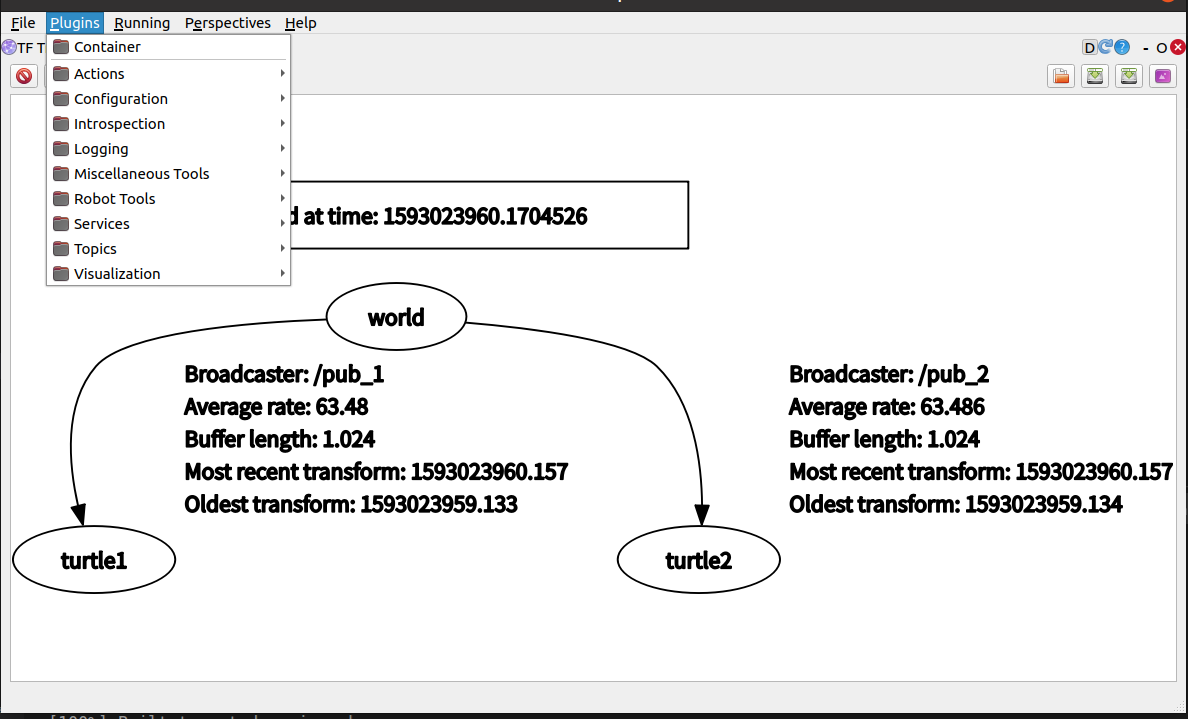
\includegraphics[width=.9\textwidth]{ros_rqt.png}
  \caption{rqt启动演示}
  \label{fig:ros_rqt}
\end{figure}

\subsection{rqt常用插件: rqt\_graph}

简介: 可视化显示计算图.

启动: 可以在 rqt 的 plugins 中添加, 或者使用 \verb|rqt_graph| 启动.

\begin{figure}[!ht]
  \centering
  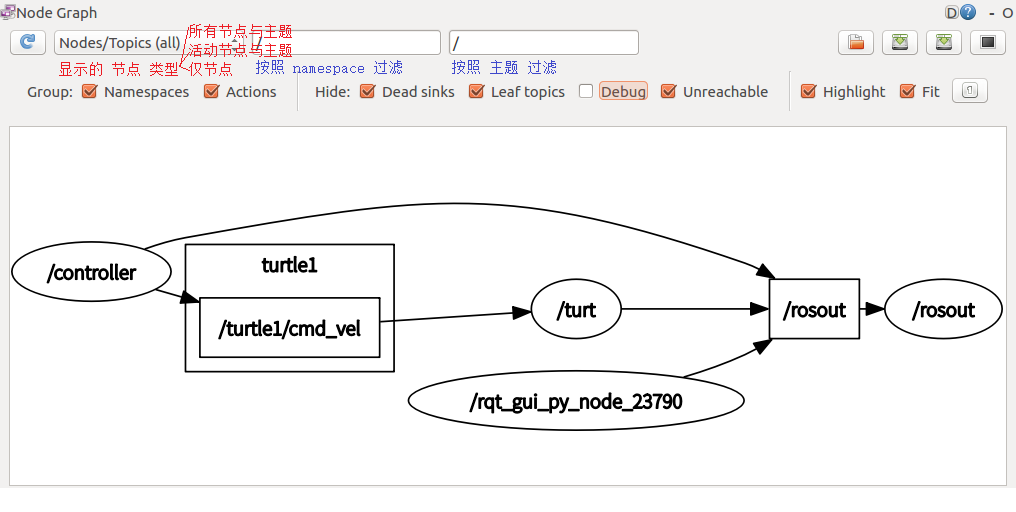
\includegraphics[width=.9\textwidth]{ros_rqt_graph.png}
  \caption{rqt\_graph启动演示}
  \label{fig:ros_rqt_graph}
\end{figure}

\subsection{rqt常用插件: rqt\_console}

简介: \verb|rqt_console| 是 ROS 中用于显示和过滤日志的图形化插件.

准备: 编写 Node 节点输出各个级别的日志信息.

\begin{cpp}
  /*  
      ROS 节点:输出各种级别的日志信息
  */

  #include "ros/ros.h"

  int main(int argc, char *argv[])
  {
      ros::init(argc,argv,"log_demo");
      ros::NodeHandle nh;
      ros::Rate r(0.3);
      while (ros::ok())
      {
          ROS_DEBUG("Debug message d");
          ROS_INFO("Info message oooooooooooooo");
          ROS_WARN("Warn message wwwww");
          ROS_ERROR("Erroe message EEEEEEEEEEEEEEEEEEEE");
          ROS_FATAL("Fatal message FFFFFFFFFFFFFFFFFFFFFFFFFFFFF");
          r.sleep();
      }
      return 0;
  }
\end{cpp}

启动: 可以在 rqt 的 plugins 中添加, 或者使用 \verb|rqt_console| 启动.

\begin{figure}[!ht]
  \centering
  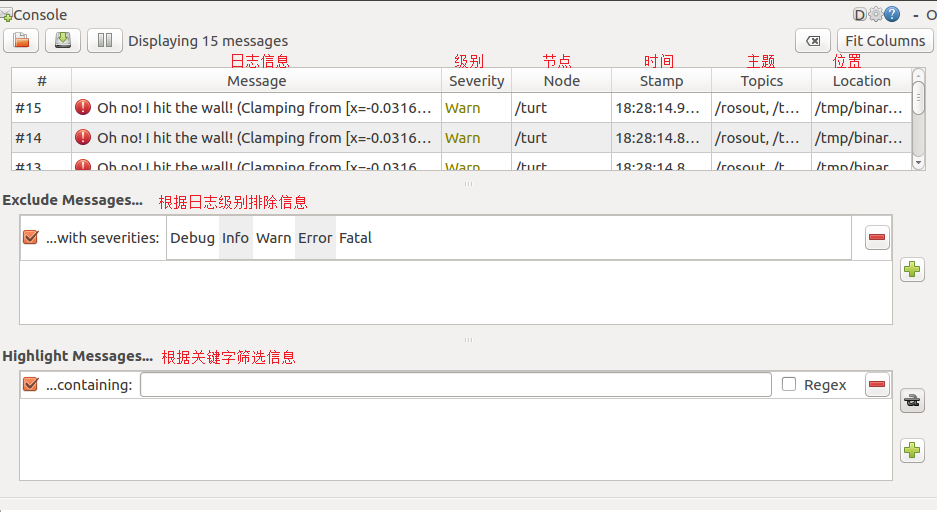
\includegraphics[width=.9\textwidth]{ros_rqt_console.png}
  \caption{rqt\_console启动演示}
  \label{fig:ros_rqt_console}
\end{figure}

\subsection{rqt常用插件: rqt\_plot}

简介: 图形绘制插件, 可以以 2D 绘图的方式绘制发布在 topic 上的数据.

准备: 启动 \verb|turtlesim| 乌龟节点与键盘控制节点, 通过 \verb|rqt_plot| 获取乌龟位姿.

启动: 可以在 rqt 的 plugins 中添加, 或者使用 \verb|rqt_plot| 启动.

\begin{figure}[!ht]
  \centering
  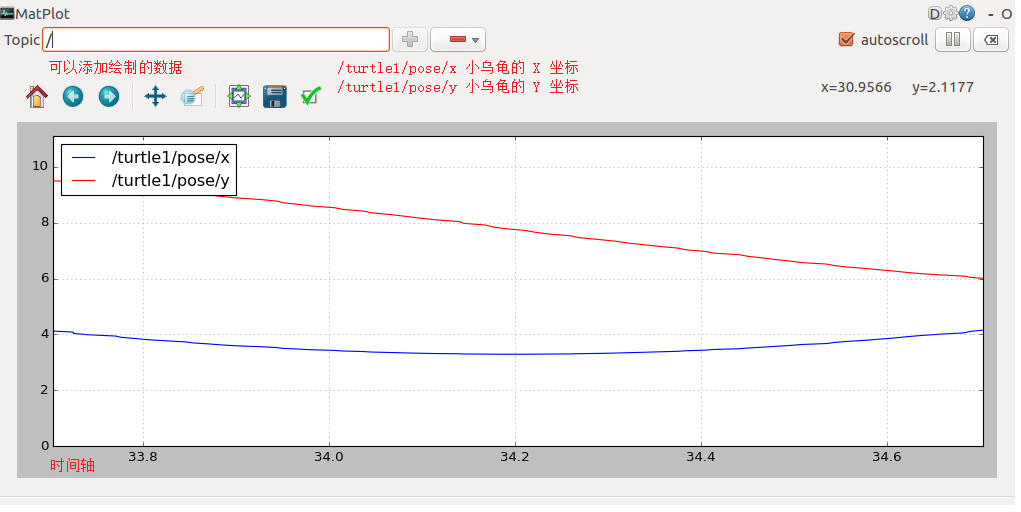
\includegraphics[width=.9\textwidth]{ros_rqt_plot.png}
  \caption{rqt\_plot启动演示}
  \label{fig:ros_rqt_plot}
\end{figure}

\subsection{rqt常用插件: rqt\_bag}

简介: 录制和重放 \verb|bag| 文件的图形化插件.

准备: 启动 \verb|turtlesim| 乌龟节点与键盘控制节点.

启动: 可以在 rqt 的 plugins 中添加, 或者使用 \verb|rqt_bag| 启动.

录制如图 \ref{fig:ros_rqt_bag_record} 所示.

\begin{figure}[!ht]
  \centering
  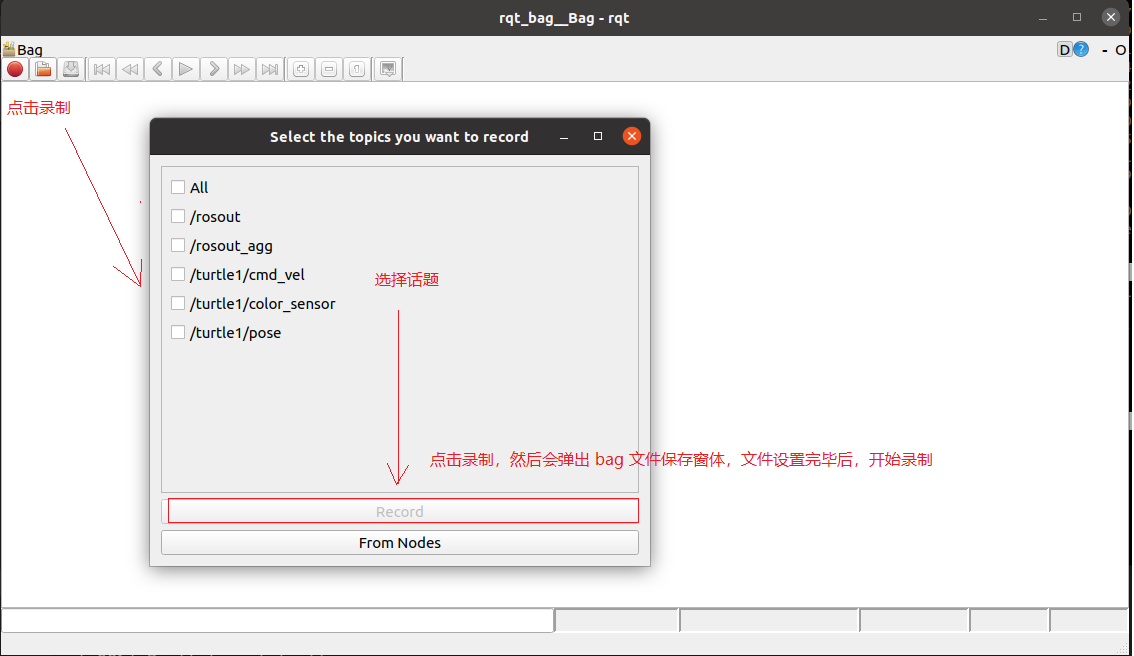
\includegraphics[width=.9\textwidth]{ros_rqt_bag_record.png}
  \caption{rqt\_bag录制演示}
  \label{fig:ros_rqt_bag_record}
\end{figure}

重放如图 \ref{fig:ros_rqt_bag_replay} 所示.

\begin{figure}[!ht]
  \centering
  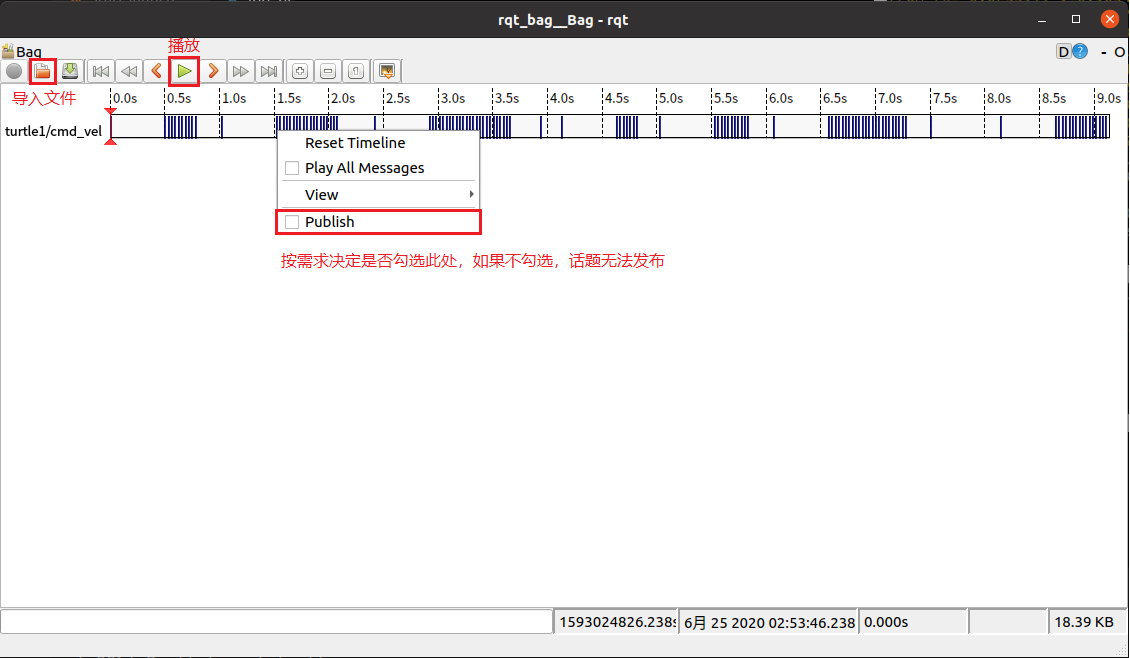
\includegraphics[width=.9\textwidth]{ros_rqt_bag_replay.png}
  \caption{rqt\_bag重放演示}
  \label{fig:ros_rqt_bag_replay}
\end{figure}

\section{本章小结}

本章主要介绍了 ROS 中的常用组件, 内容如下:

\begin{itemize}
  \item TF坐标变换 (重点);
  \item \verb|rosbag| 用于 ROS 话题的录制与回放;
  \item rqt 工具箱, 图形化方式调用组件, 提高操作效率以及易用性.
\end{itemize}

其中, TF 坐标变换是重点, 也是难点, 需要大家熟练掌握坐标变换的应用场景以及代码实现. 下一章开始将介绍机器人系统仿真, 我们将在仿真环境下, 创建机器人、控制机器人运动、搭建仿真环境, 并以机器人的视角去感知世界.

\chapter{机器人系统仿真}
\label{chapter:robot_simulation}

对于 ROS 新手而言, 可能会有疑问: 学习机器人操作系统, 实体机器人是必须的吗? 答案是否定的, 机器人一般价格不菲, 为了降低机器人学习、调试成本, 在 ROS 中提供了系统的机器人仿真实现, 通过仿真, 可以实现大部分需求, 本章主要就是围绕仿真展开的, 比如, 本章会介绍:

\begin{itemize}
  \item 如何创建并显示机器人模型; 
  \item 如何搭建仿真环境; 
  \item 如何实现机器人模型与仿真环境的交互.
\end{itemize}

本章预期的学习目标如下:

\begin{itemize}
  \item 能够独立使用 URDF 创建机器人模型, 并在 RViz 和 Gazebo 中分别显示; 
  \item 能够使用 Gazebo 搭建仿真环境; 
  \item 能够使用机器人模型中的传感器 (雷达、摄像头、编码器等等) 获取仿真环境数据.
\end{itemize}

案例演示:

1. 创建并显示机器人模型, 如图 \ref{fig:ros_sim_create_robot} 与图 \ref{fig:ros_sim_show_robot} 所示.

\begin{figure}[!ht]
  \centering
  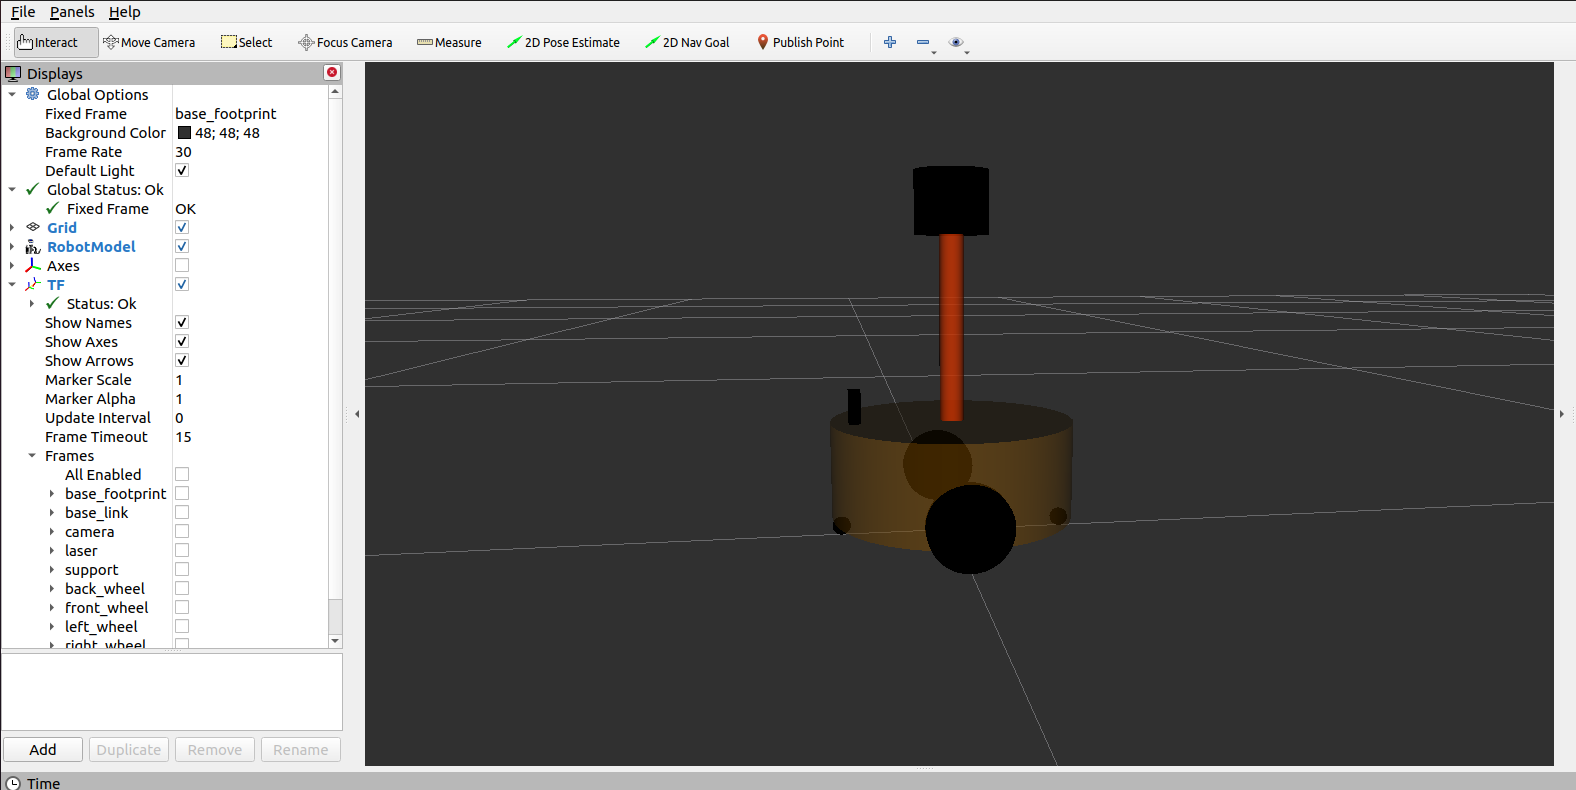
\includegraphics[width=.9\textwidth]{ros_sim_create_robot.png}
  \caption{创建机器人模型}
  \label{fig:ros_sim_create_robot}
\end{figure}

\begin{figure}[!ht]
  \centering
  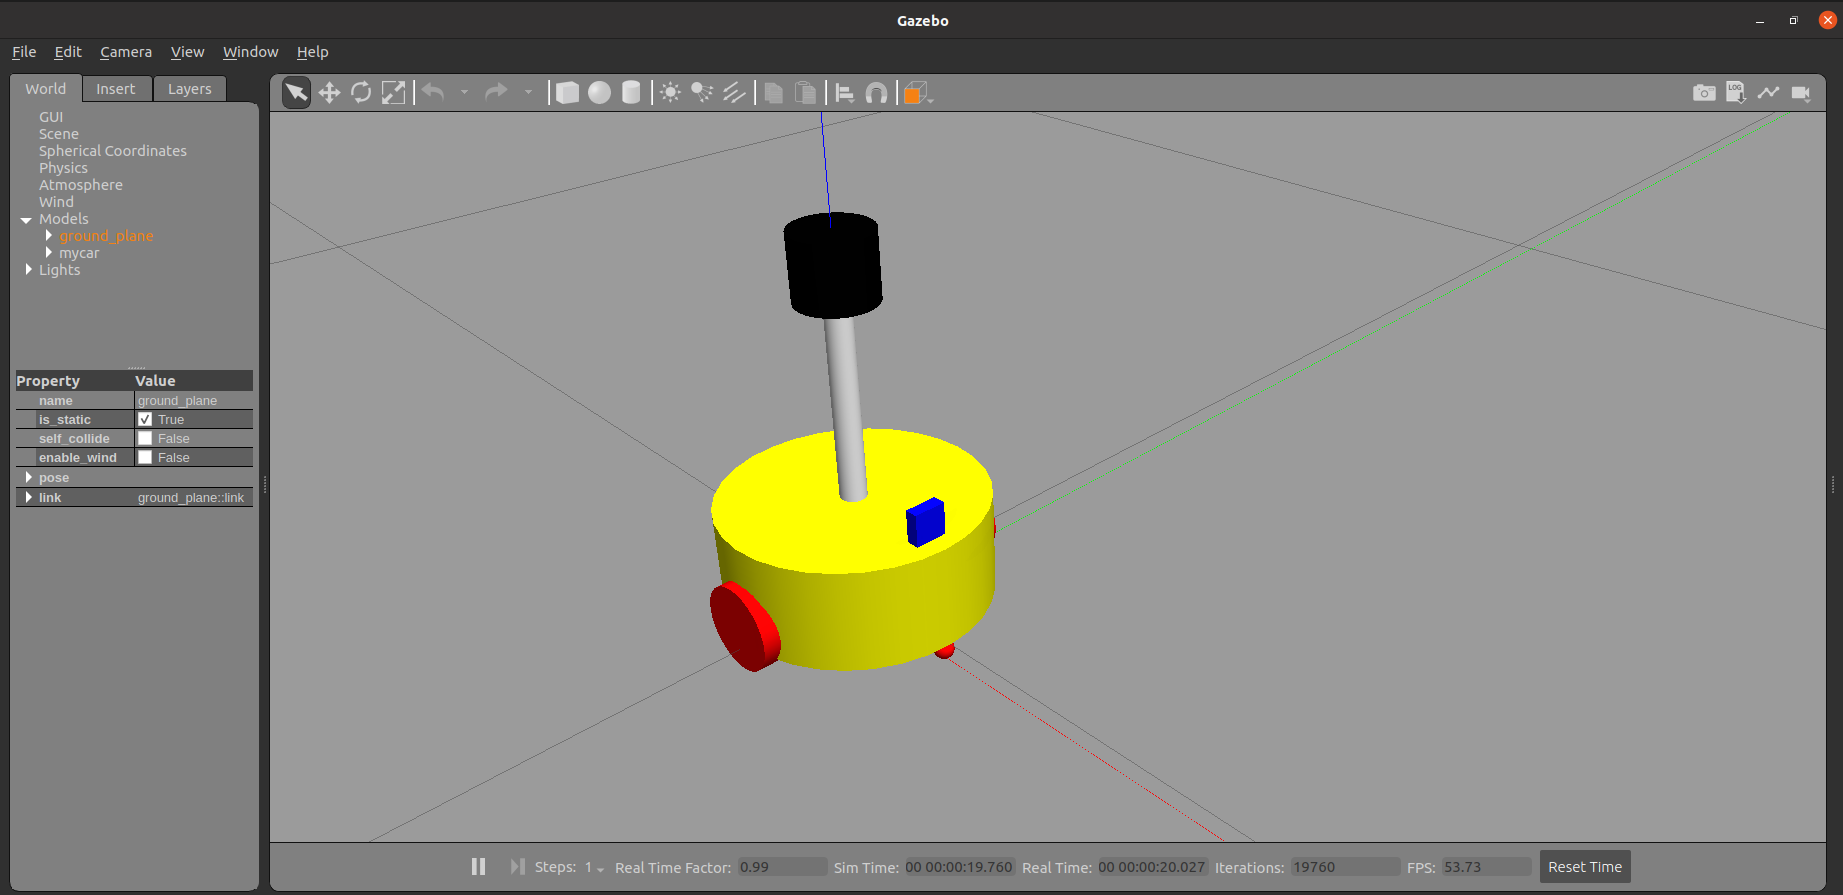
\includegraphics[width=.9\textwidth]{ros_sim_show_robot.png}
  \caption{显示机器人模型}
  \label{fig:ros_sim_show_robot}
\end{figure}

2. 仿真环境搭建, 如图 \ref{fig:ros_sim_build_env} 所示.

\begin{figure}[!ht]
  \centering
  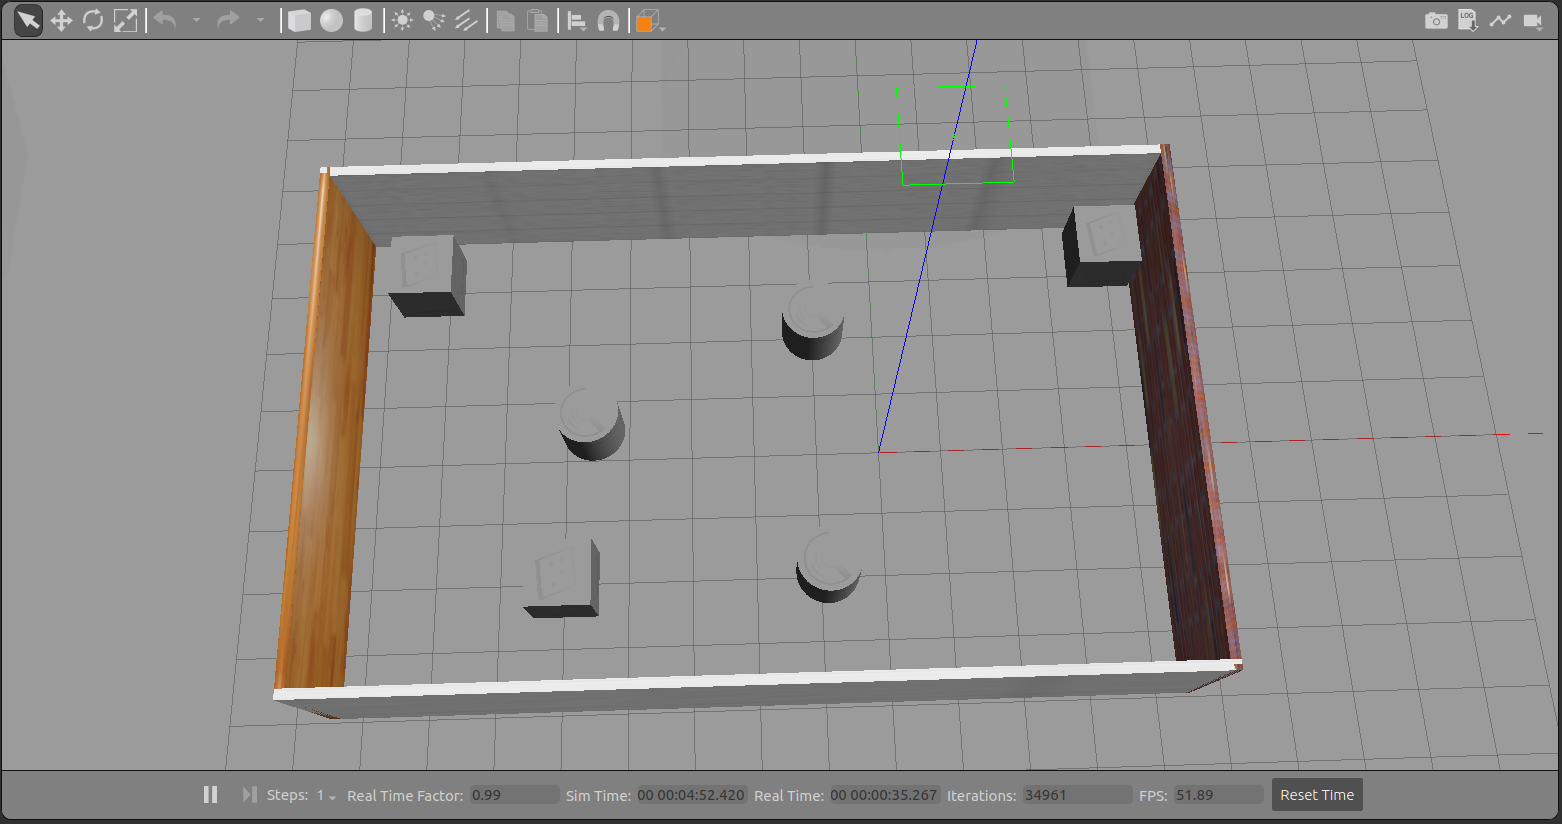
\includegraphics[width=.9\textwidth]{ros_sim_build_env.png}
  \caption{仿真环境搭建}
  \label{fig:ros_sim_build_env}
\end{figure}

3. 控制机器人运动, 如图 \ref{fig:ros_sim_control_robot_local} 与图 \ref{fig:ros_sim_control_robot_global} 所示.

\begin{figure}[!ht]
  \centering
  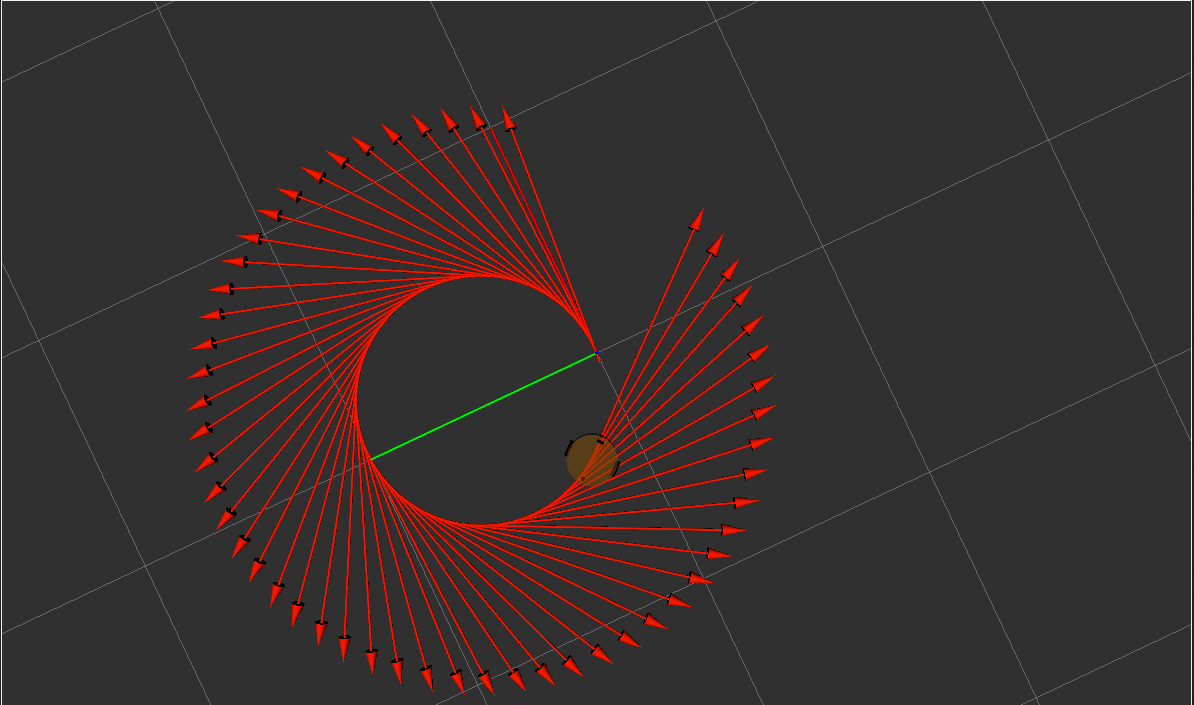
\includegraphics[width=.7\textwidth]{ros_sim_control_robot_local.png}
  \caption{控制机器人运动01}
  \label{fig:ros_sim_control_robot_local}
\end{figure}

\begin{figure}[!ht]
  \centering
  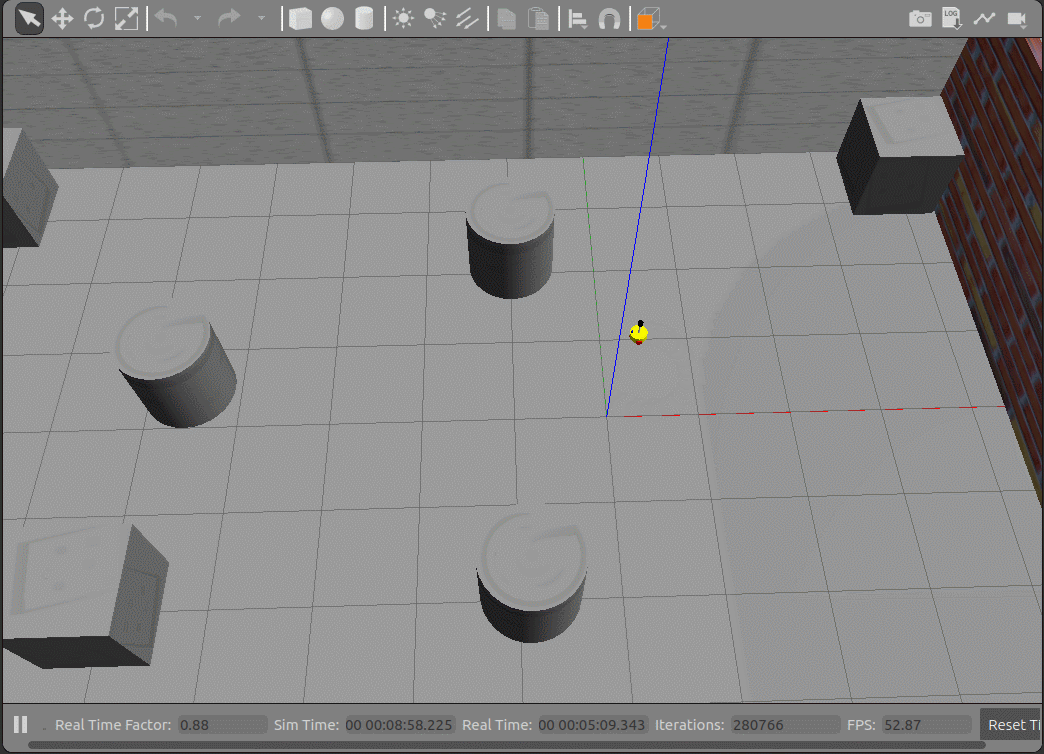
\includegraphics[width=.7\textwidth]{ros_sim_control_robot_global.png}
  \caption{控制机器人运动02}
  \label{fig:ros_sim_control_robot_global}
\end{figure}

4. 雷达仿真, 如图 \ref{fig:ros_sim_lidar} 所示.

\begin{figure}[!ht]
  \centering
  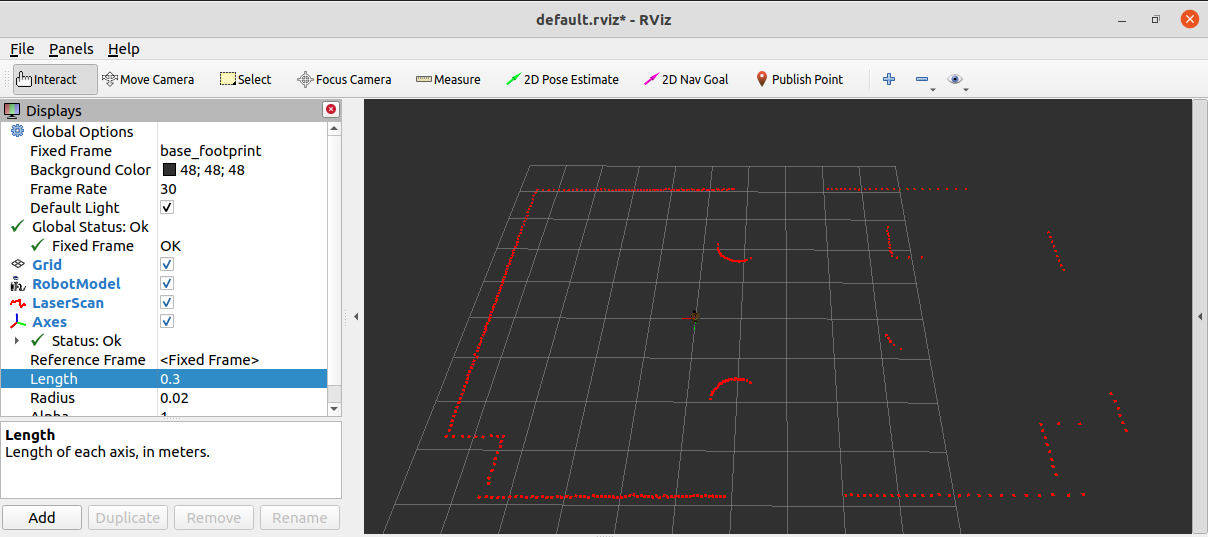
\includegraphics[width=.9\textwidth]{ros_sim_lidar.png}
  \caption{雷达仿真}
  \label{fig:ros_sim_lidar}
\end{figure}

5. 摄像头仿真, 如图 \ref{fig:ros_sim_camera_01} 和 图 \ref{fig:ros_sim_camera_02} 所示.

\begin{figure}[!ht]
  \centering
  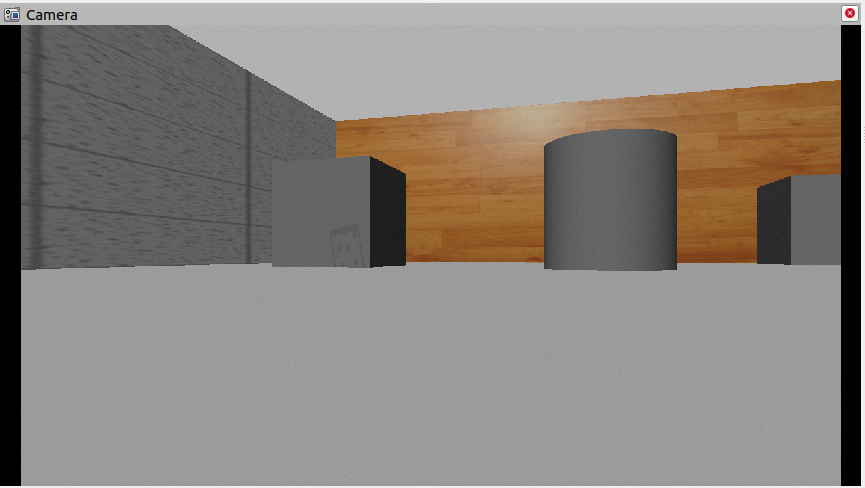
\includegraphics[width=.9\textwidth]{ros_sim_camera_01.png}
  \caption{摄像头仿真01}
  \label{fig:ros_sim_camera_01}
\end{figure}

\begin{figure}[!ht]
  \centering
  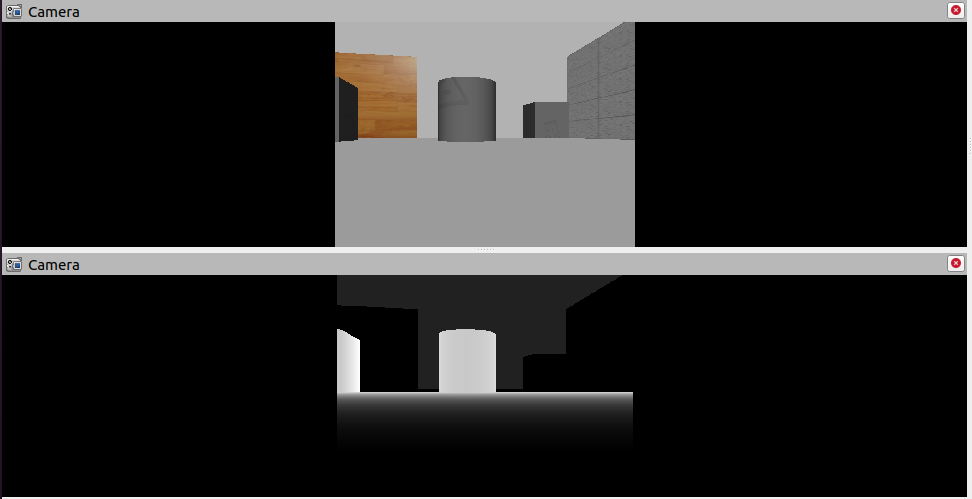
\includegraphics[width=.9\textwidth]{ros_sim_camera_02.png}
  \caption{摄像头仿真02}
  \label{fig:ros_sim_camera_02}
\end{figure}

\section{概述}

机器人操作系统学习、开发与测试过程中, 会遇到诸多问题, 比如:

\begin{itemize}
  \item 机器人一般价格不菲, 学习 ROS 要购买一台机器人吗? 
  \item 机器人与之交互的外界环境具有多样性, 如何实现复杂的环境设计?
  \item 测试时, 直接将未经验证的程序部署到实体机器人运行, 安全吗?
\end{itemize}

在诸如此类的场景中, ROS 中的仿真就显得尤为重要了.

1. 概念

机器人系统仿真: 是通过计算机对实体机器人系统进行模拟的技术, 在 ROS 中, 仿真实现涉及的内容主要有三: 对机器人建模 (URDF)、创建仿真环境 (Gazebo) 以及感知环境 (RViz) 等系统性实现.

2. 作用

2.1 仿真优势

仿真在机器人系统研发过程中占有举足轻重的地位, 在研发与测试中较之于实体机器人实现, 仿真有如下几点的显著优势:

\begin{itemize}
  \item 低成本: 当前机器人成本居高不下, 动辄几十万, 仿真可以大大降低成本, 减小风险;
  \item 高效: 搭建的环境更为多样且灵活, 可以提高测试效率以及测试覆盖率;
  \item 高安全性: 仿真环境下, 无需考虑耗损问题.
\end{itemize}

2.2 仿真缺陷

机器人在仿真环境与实际环境下的表现差异较大, 换言之, 仿真并不能完全做到模拟真实的物理世界, 存在一些失真的情况, 原因:

\begin{itemize}
  \item 仿真器所使用的物理引擎目前还不能够完全精确模拟真实世界的物理情况;
  \item 仿真器构建的是关节驱动器 (电机与齿轮箱) 、传感器与信号通信的绝对理想情况, 目前不支持模拟实际硬件缺陷或者一些临界状态等情形.
\end{itemize}

3. 相关组件

3.1 URDF

URDF是 Unified Robot Description Format 的首字母缩写, 直译为统一 (标准化) 机器人描述格式, 可以以一种 XML 的方式描述机器人的部分结构, 比如底盘、摄像头、激光雷达、机械臂以及不同关节的自由度等等, 该文件可以被 C++ 内置的解释器转换成可视化的机器人模型, 是 ROS 中实现机器人仿真的重要组件

3.2 RViz

RViz 是 ROS Visualization Tool 的首字母缩写, 直译为 ROS 的三维可视化工具. 它的主要目的是以三维方式显示 ROS 消息, 可以将数据进行可视化表达. 例如:可以显示机器人模型, 可以无需编程就能表达激光测距仪 (LRF) 传感器中的传感 器到障碍物的距离, RealSense、Kinect 或 Xtion 等三维距离传感器的点云数据 (PCD, Point Cloud Data) , 从相机获取的图像值等.

以 \verb|ros-[ROS_DISTRO]-desktop-full| 命令安装 ROS 时, RViz会默认被安装. 运行使用命令 \verb|rviz| 或 \verb|rosrun rviz rviz|. 如果 RViz 没有安装, 请调用如下命令自行安装:

\begin{bash}
  sudo apt install ros-[ROS_DISTRO]-rviz
\end{bash}

3.3 Gazebo

Gazebo 是一款3D动态模拟器, 用于显示机器人模型并创建仿真环境, 能够在复杂的室内和室外环境中准确有效地模拟机器人. 与游戏引擎提供高保真度的视觉模拟类似, Gazebo 提供高保真度的物理模拟, 其提供一整套传感器模型, 以及对用户和程序非常友好的交互方式.

以 \verb|ros-[ROS_DISTRO]-desktop-full| 命令安装 ROS 时, Gazebo 会默认被安装. 运行使用命令 \verb|gazebo| 或 \verb|rosrun gazebo_ros gazebo|. 如果 Gazebo 没有安装, 请自行安装:

1. 添加源:

\begin{bash}
  sudo sh -c 'echo "deb http://packages.osrfoundation.org/gazebo/ubuntu-stable `lsb_release -cs` main" > /etc/apt/sources.list.d/gazebo-stable.list'
  wget http://packages.osrfoundation.org/gazebo.key -O - | sudo apt-key add -
\end{bash}

2. 安装: 

\begin{bash}
  sudo apt update
  sudo apt install gazebo11 
  sudo apt install libgazebo11-dev
\end{bash}

机器人的系统仿真是一种集成实现, 主要包含三部分:

\begin{itemize}
  \item URDF 用于创建机器人模型;
  \item Gazebo 用于搭建仿真环境;
  \item RViz 图形化的显示机器人各种传感器感知到的环境信息.
\end{itemize}

三者应用中, 只是创建 URDF 意义不大, 一般需要结合 Gazebo 或 RViz 使用, 在 Gazebo 或 RViz 中可以将 URDF 文件解析为图形化的机器人模型, 一般的使用组合为:

\begin{itemize}
  \item 如果非仿真环境, 那么使用 URDF 结合 RViz 直接显示感知的真实环境信息;
  \item 如果是仿真环境, 那么需要使用 URDF 结合 Gazebo 搭建仿真环境, 并结合 RViz 显示感知的虚拟环境信息.
\end{itemize}

后续课程安排:

\begin{itemize}
  \item 先介绍 URDF 与 RViz 集成使用, 在 RViz 中只是显示机器人模型, 主要用于学习 URDF 语法;
  \item 再介绍 URDF 与 Gazebo 集成, 主要学习 URDF 仿真相关语法以及仿真环境搭建;
  \item 最后集成 URDF 与 Gazebo 与 RViz, 实现综合应用.
\end{itemize}

素材 \href{https://github.com/zx595306686/sim_demo.git}{链接}.

\section{URDF集成RViz基本流程}

前面介绍过, URDF 不能单独使用, 需要结合 RViz 或 Gazebo, URDF 只是一个文件, 需要在 RViz 或 Gazebo 中渲染成图形化的机器人模型, 当前, 首先演示 URDF 与 RViz 的集成使用, 因为 URDF 与 RViz 的集成较之于 URDF 与 Gazebo 的集成更为简单, 后期, 基于 RViz 的集成实现, 我们再进一步介绍 URDF 语法.

需求描述: 在 RViz 中显示一个盒状机器人.

结果演示:

\begin{figure}[!ht]
  \centering
  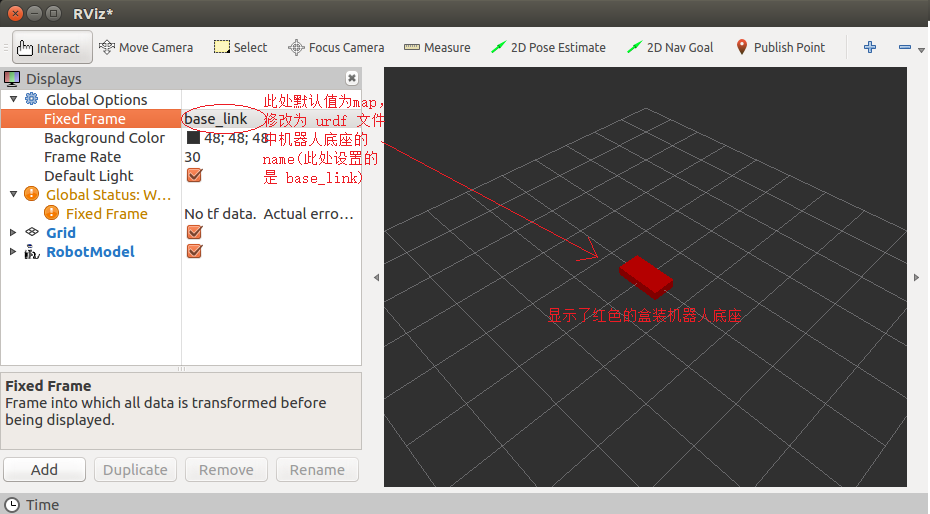
\includegraphics[width=.9\textwidth]{ros_sim_urdf_rviz.png}
  \caption{URDF集成RViz结果演示}
  \label{fig:ros_sim_urdf_rviz}
\end{figure}

实现流程: 

\begin{itemize}
  \item 准备: 新建功能包, 导入依赖;
  \item 核心: 编写 URDF 文件;
  \item 核心: 在 launch 文件集成 URDF 与 RViz;
  \item 在 RViz 中显示机器人模型.
\end{itemize}

1. 创建功能包, 导入依赖

创建一个新的功能包, 名称自定义, 导入依赖包:

\begin{bash}
  catkin_create_pkg your_ros_package urdf xacro
\end{bash}

在当前功能包下, 再新建几个目录:

\begin{itemize}
  \item \verb|urdf|: 存储 URDF 文件的目录;
  \item \verb|umeshes|: 机器人模型渲染文件 (暂不使用);
  \item \verb|uconfig|: 配置文件;
  \item \verb|ulaunch|: 存储 launch 启动文件.
\end{itemize}

2. 编写 URDF 文件

新建一个子级文件夹: \verb|urdf| (可选), 文件夹中添加一个 \verb|.urdf| 文件, 复制如下内容:

\begin{xml}
  <robot name="mycar">
      <link name="base_link">
          <visual>
              <geometry>
                  <box size="0.5 0.2 0.1" />
              </geometry>
          </visual>
      </link>
  </robot>
\end{xml}

3. 在 launch 文件中集成 URDF 与 RViz

在launch目录下, 新建一个 launch 文件, 该 launch 文件需要启动 RViz, 并导入 URDF 文件, RViz 启动后可以自动载入解析 URDF 文件, 并显示机器人模型, 核心问题: 如何导入 URDF 文件? 在 ROS 中, 可以将 URDF 文件的路径设置到参数服务器, 使用的参数名是: \verb|robot_description|, 示例代码如下:

\begin{xml}
  <launch>
      <!-- 设置参数 -->
      <param name="robot_description" textfile="$(find 包名)/urdf/urdf/urdf01_HelloWorld.urdf" />
      <!-- 启动 rviz -->
      <node pkg="rviz" type="rviz" name="rviz" />
  </launch>
\end{xml}

4. 在 RViz 中显示机器人模型

RViz 启动后, 会发现并没有盒装的机器人模型, 这是因为默认情况下没有添加机器人显示组件, 需要手动添加, 添加方式如图 \ref{fig:ros_sim_urdf_rviz_setting_01} 所示. 设置完毕后, 可以正常显示了, 如图 \ref{fig:ros_sim_urdf_rviz_setting_02} 所示.

\begin{figure}[!ht]
  \centering
  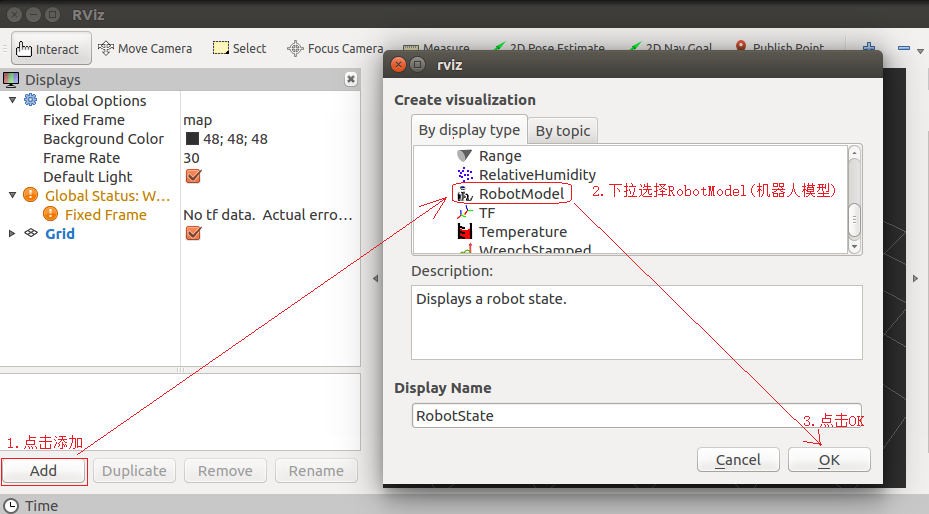
\includegraphics[width=.9\textwidth]{ros_sim_urdf_rviz_setting_01.png}
  \caption{RViz显示机器人模型 (添加显示)}
  \label{fig:ros_sim_urdf_rviz_setting_01}
\end{figure}

\begin{figure}[!ht]
  \centering
  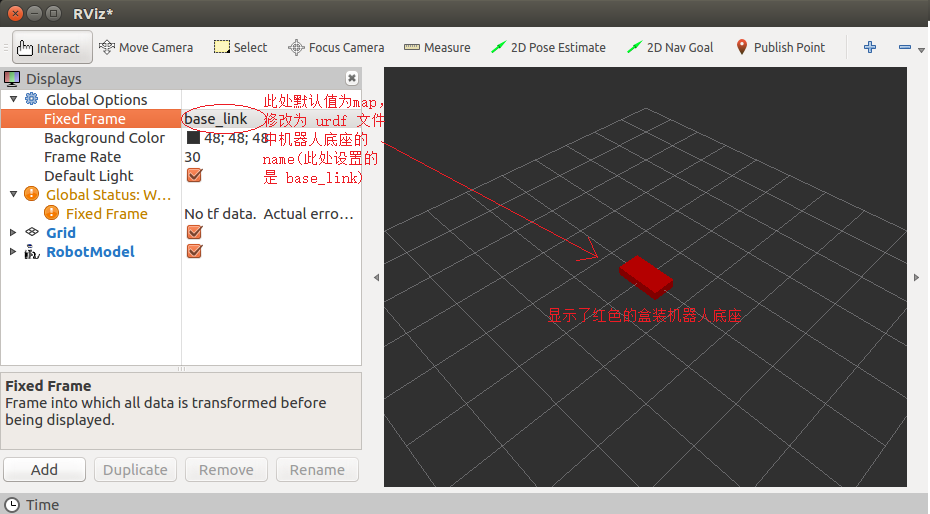
\includegraphics[width=.9\textwidth]{ros_sim_urdf_rviz_setting_02.png}
  \caption{RViz显示机器人模型}
  \label{fig:ros_sim_urdf_rviz_setting_02}
\end{figure}

5. 优化 RViz 启动

重复启动 launch 文件时, RViz 之前的组件配置信息不会自动保存, 需要重复执行步骤4的操作, 为了方便使用, 可以使用如下方式优化:

首先, 将当前配置保存进 \verb|config| 目录然后, launch 文件中 RViz 的启动配置添加参数 \verb|:args|, 值设置为 \verb|-d 配置文件路径|.

\begin{xml}
  <launch>
      <param name="robot_description" textfile="$(find 包名)/urdf/urdf/urdf01_HelloWorld.urdf" />
      <node pkg="rviz" type="rviz" name="rviz" args="-d $(find 包名)/config/rviz/show_mycar.rviz" />
  </launch>
\end{xml}

\begin{figure}[!ht]
  \centering
  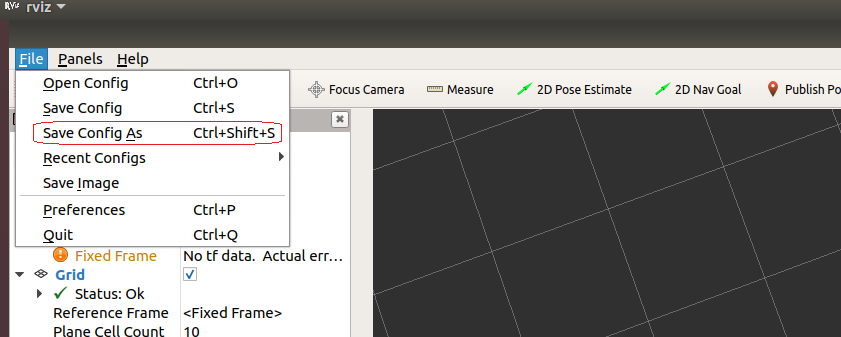
\includegraphics[width=.9\textwidth]{ros_sim_urdf_rviz_save_config.png}
  \caption{RViz配置保存}
  \label{fig:ros_sim_urdf_rviz_save_config}
\end{figure}

再启动时, 就可以包含之前的组件配置了, 使用更方便快捷.

\section{URDF语法详解}

URDF 文件是一个标准的 XML 文件, 在 ROS 中预定义了一系列的标签用于描述机器人模型, 机器人模型可能较为复杂, 但是 ROS 的 URDF 中机器人的组成却是较为简单, 可以主要简化为两部分: 连杆 (\verb|link| 标签) 与 关节 (\verb|joint| 标签), 接下来我们就通过案例了解一下 URDF 中的不同标签:

\begin{itemize}
  \item \verb|robot|: 根标签, 类似于 launch 文件中的 \verb|launch| 标签
  \item \verb|link|: 连杆标签
  \item \verb|joint|: 关节标签
  \item \verb|gazebo|: 集成 Gazebo 需要使用的标签
\end{itemize}

关于 \verb|gazebo| 标签, 后期在使用 Gazebo 仿真时, 才需要使用到, 用于配置仿真环境所需参数, 比如: 机器人材料属性、Gazebo 插件等, 但是该标签不是机器人模型必须的, 只有在仿真时才需设置.

\subsection{URDF语法详解: robot}

URDF 中为了保证 XML 语法的完整性, 使用了 \verb|robot| 标签作为根标签, 所有的 \verb|link| 和 \verb|joint| 以及其他标签都必须包含在 \verb|robot| 标签内, 在该标签内可以通过 \verb|name| 属性设置机器人模型的名称.

1. 属性

\begin{itemize}
  \item \verb|name|: 指定机器人模型的名称.
\end{itemize}

2. 子标签

其他标签都是子级标签.

\subsection{URDF语法详解: link}

URDF 中的 \verb|link| 标签用于描述机器人某个部件 (也即刚体部分) 的外观和物理属性, 比如: 机器人底座、轮子、激光雷达、摄像头...每一个部件都对应一个 \verb|link|, 在 \verb|link| 标签内, 可以设计该部件的形状、尺寸、颜色、惯性矩阵、碰撞参数等一系列属性.

\begin{figure}[!ht]
  \centering
  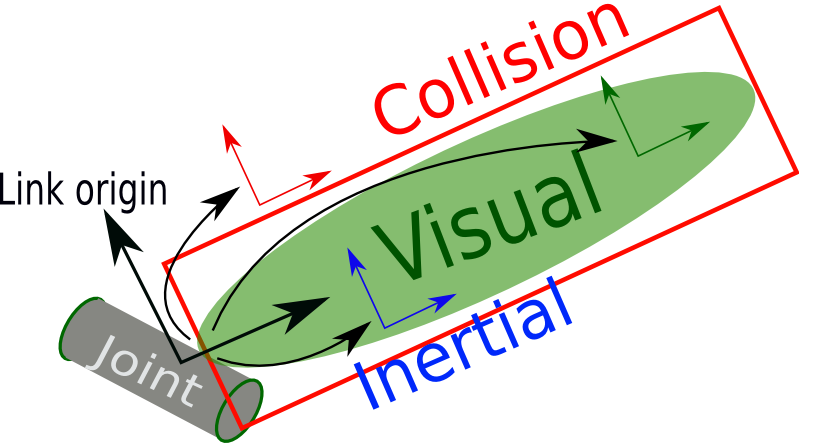
\includegraphics[width=.3\textwidth]{robot_link.png}
  \caption{机器人link示意}
  \label{fig:robot_link}
\end{figure}

1. 属性

\begin{itemize}
  \item \verb|name|: 为连杆命名
\end{itemize}

2. 子标签

\begin{itemize}
  \item \verb|visual|: 描述外观 (对应的数据是可视的)
  \item \verb|geometry|: 设置连杆的形状
  \begin{itemize}
    \item 标签1: \verb|box| (盒状), 属性: \verb|size=长 (x) 宽 (y) 高 (z)|
    \item 标签2: \verb|cylinder| (圆柱), 属性: \verb|radius=半径 length=高度|
    \item 标签3: \verb|sphere| (球体), 属性: \verb|radius=半径|
    \item 标签4: \verb|mesh| (为连杆添加皮肤), 属性: \verb|filename=资源路径| 
    
    (格式: \verb|package://<packagename>/<path>/文件|)
  \end{itemize}
  \item \verb|origin|: 设置偏移量与倾斜弧度
  \begin{itemize}
    \item 属性1: \verb|xyz=x偏移 y便宜 z偏移|
    \item 属性2: \verb|rpy=x翻滚 y俯仰 z偏航| (单位是弧度)
  \end{itemize}
  \item \verb|metrial|: 设置材料属性 (颜色)
  \begin{itemize}
    \item 属性: \verb|name|
    \item 标签: \verb|color|, 属性: \verb|rgba=红绿蓝权重值与透明度| (每个权重值以及透明度取值[0,1])
  \end{itemize}
  \item \verb|collision|: 连杆的碰撞属性
  \item \verb|Inertial|: 连杆的惯性矩阵
\end{itemize}

在此, 只演示 \verb|visual| 使用.

3. 案例

需求: 分别生成长方体、圆柱与球体的机器人部件.

\begin{xml}
  <link name="base_link">
      <visual>
          <!-- 形状 -->
          <geometry>
              <!-- 长方体的长宽高 -->
              <!-- <box size="0.5 0.3 0.1" /> -->
              <!-- 圆柱, 半径和长度 -->
              <!-- <cylinder radius="0.5" length="0.1" /> -->
              <!-- 球体, 半径-->
              <!-- <sphere radius="0.3" /> -->

          </geometry>
          <!-- xyz坐标 rpy翻滚俯仰与偏航角度 (3.14=180度 1.57=90度) -->
          <origin xyz="0 0 0" rpy="0 0 0" />
          <!-- 颜色: r=red g=green b=blue a=alpha -->
          <material name="black">
              <color rgba="0.7 0.5 0 0.5" />
          </material>
      </visual>
  </link>
\end{xml}

\subsection{URDF语法详解: joint}

URDF 中的 \verb|joint| 标签用于描述机器人关节的运动学和动力学属性, 还可以指定关节运动的安全极限, 机器人的两个部件 (分别称之为 parent link 与 child link) 以关节的形式相连接, 不同的关节有不同的运动形式: 旋转、滑动、固定、旋转速度、旋转角度限制等等, 比如:安装在底座上的轮子可以 360 度旋转, 而摄像头则可能是完全固定在底座上.

\begin{figure}[!ht]
  \centering
  \includegraphics[width=.4\textwidth]{robot_joint.png}
  \caption{机器人joint示意}
  \label{fig:robot_joint}
\end{figure}

\verb|joint| 标签对应的数据在模型中是不可见的.

1. 属性

\begin{itemize}
  \item \verb|name|: 为关节命名;
  \item \verb|type|: 关节运动形式;
  \begin{itemize}
    \item \verb|continuous|: 旋转关节, 可以绕单轴无限旋转;
    \item \verb|revolute|: 旋转关节, 类似于 \verb|continues|, 但是有旋转角度限制;
    \item \verb|prismatic|: 滑动关节, 沿某一轴线移动的关节, 有位置极限;
    \item \verb|planer|: 平面关节, 允许在平面正交方向上平移或旋转;
    \item \verb|floating|: 浮动关节, 允许进行平移、旋转运动;
    \item \verb|fixed|: 固定关节, 不允许运动的特殊关节.
  \end{itemize}
\end{itemize}

2. 子标签

\begin{itemize}
  \item \verb|parent| (必需的): \verb|parent link| 的名字是一个强制的属性: \verb|link|: 父级连杆的名字, 是这个 \verb|link| 在机器人结构树中的名字.
  \item \verb|child| (必需的): \verb|child link| 的名字是一个强制的属性: \verb|link|: 子级连杆的名字, 是这个 \verb|link| 在机器人结构树中的名字.
  \item \verb|origin|: 属性: \verb|xyz=各轴线上的偏移量| \verb|rpy=各轴线上的偏移弧度|.
  \item \verb|axis|: 属性: \verb|xyz用于设置围绕哪个关节轴运动|.
\end{itemize}

3. 案例

需求: 创建机器人模型, 底盘为长方体, 在长方体的前面添加一摄像头, 摄像头可以沿着 $Z$ 轴 360 度旋转.

URDF 文件示例如下:

\begin{xml}
  <!-- 
      需求: 创建机器人模型, 底盘为长方体, 
          在长方体的前面添加一摄像头, 
          摄像头可以沿着 Z 轴 360 度旋转
  -->
  <robot name="mycar">
      <!-- 底盘 -->
      <link name="base_link">
          <visual>
              <geometry>
                  <box size="0.5 0.2 0.1" />
              </geometry>
              <origin xyz="0 0 0" rpy="0 0 0" />
              <material name="blue">
                  <color rgba="0 0 1.0 0.5" />
              </material>
          </visual>
      </link>
      <!-- 摄像头 -->
      <link name="camera">
          <visual>
              <geometry>
                  <box size="0.02 0.05 0.05" />
              </geometry>
              <origin xyz="0 0 0" rpy="0 0 0" />
              <material name="red">
                  <color rgba="1 0 0 0.5" />
              </material>
          </visual>
      </link>
      <!-- 关节 -->
      <joint name="camera2baselink" type="continuous">
          <parent link="base_link"/>
          <child link="camera" />
          <!-- 需要计算两个 link 的物理中心之间的偏移量 -->
          <origin xyz="0.2 0 0.075" rpy="0 0 0" />
          <axis xyz="0 0 1" />
      </joint>
  </robot>
\end{xml}

launch文件示例如下:

\begin{xml}
  <launch>
      <param name="robot_description" textfile="$(find urdf_rviz_demo)/urdf/urdf/urdf03_joint.urdf" />
      <node pkg="rviz" type="rviz" name="rviz" args="-d $(find urdf_rviz_demo)/config/helloworld.rviz" /> 
      <!-- 添加关节状态发布节点 -->
      <node pkg="joint_state_publisher" type="joint_state_publisher" name="joint_state_publisher" />
      <!-- 添加机器人状态发布节点 -->
      <node pkg="robot_state_publisher" type="robot_state_publisher" name="robot_state_publisher" />
      <!-- 可选:用于控制关节运动的节点 -->
      <node pkg="joint_state_publisher_gui" type="joint_state_publisher_gui" name="joint_state_publisher_gui" />
  </launch>
\end{xml}

PS:

1. 状态发布节点在此是必须的:

\begin{xml}
  <!-- 添加关节状态发布节点 -->
  <node pkg="joint_state_publisher" type="joint_state_publisher" name="joint_state_publisher" />
  <!-- 添加机器人状态发布节点 -->
  <node pkg="robot_state_publisher" type="robot_state_publisher" name="robot_state_publisher" />
\end{xml}

2. 关节运动控制节点 (可选), 会生成关节控制的UI, 用于测试关节运动是否正常.

\begin{xml}
  <!-- 可选:用于控制关节运动的节点 -->
  <node pkg="joint_state_publisher_gui" type="joint_state_publisher_gui" name="joint_state_publisher_gui" />
\end{xml}

4. \verb|base_footprint| 优化 URDF

前面实现的机器人模型是半沉到地下的, 因为默认情况下: 底盘的中心点位于地图原点上, 所以会导致这种情况产生, 可以使用的优化策略, 将初始 \verb|link| 设置为一个尺寸极小的 \verb|link| (比如半径为 0.001m 的球体, 或边长为 0.001m 的立方体), 然后再在初始 \verb|link| 上添加底盘等刚体, 这样实现, 虽然仍然存在初始 \verb|link| 半沉的现象, 但是基本可以忽略了. 这个初始 \verb|link| 一般称之为 \verb|base_footprint|.

\begin{xml}
  <!-- 使用 base_footprint 优化 -->
  <robot name="mycar">
      <!-- 设置一个原点 (机器人中心点的投影) -->
      <link name="base_footprint">
          <visual>
              <geometry>
                  <sphere radius="0.001" />
              </geometry>
          </visual>
      </link>
      <!-- 添加底盘 -->
      <link name="base_link">
          <visual>
              <geometry>
                  <box size="0.5 0.2 0.1" />
              </geometry>
              <origin xyz="0 0 0" rpy="0 0 0" />
              <material name="blue">
                  <color rgba="0 0 1.0 0.5" />
              </material>
          </visual>
      </link>
      <!-- 底盘与原点连接的关节 -->
      <joint name="base_link2base_footprint" type="fixed">
          <parent link="base_footprint" />
          <child link="base_link" />
          <origin xyz="0 0 0.05" />
      </joint>
      <!-- 添加摄像头 -->
      <link name="camera">
          <visual>
              <geometry>
                  <box size="0.02 0.05 0.05" />
              </geometry>
              <origin xyz="0 0 0" rpy="0 0 0" />
              <material name="red">
                  <color rgba="1 0 0 0.5" />
              </material>
          </visual>
      </link>
      <!-- 关节 -->
      <joint name="camera2baselink" type="continuous">
          <parent link="base_link"/>
          <child link="camera" />
          <origin xyz="0.2 0 0.075" rpy="0 0 0" />
          <axis xyz="0 0 1" />
      </joint>
  </robot>
\end{xml}

launch 文件内容不变.

5. 遇到问题以及解决

问题1: 命令行输出如下错误提示:

\begin{bash}
  UnicodeEncodeError: 'ascii' codec can't encode characters in position 463-464: ordinal not in range(128)
  [joint_state_publisher-3] process has died [pid 4443, exit code 1, cmd /opt/ros/melodic/lib/joint_state_publisher/joint_state_publisher __name:=joint_state_publisher __log:=/home/rosmelodic/.ros/log/b38967c0-0acb-11eb-aee3-0800278ee10c/joint_state_publisher-3.log].
  log file: /home/rosmelodic/.ros/log/b38967c0-0acb-11eb-aee3-0800278ee10c/joint_state_publisher-3*.log
\end{bash}

RViz 中提示坐标变换异常, 导致机器人部件显示结构异常.

原因: 编码问题导致的.

解决: 去除 URDF 中的中文注释.

问题2: 

\begin{bash}
  [ERROR] [1584370263.037038]: Could not find the GUI, install the 'joint_state_publisher_gui' package
\end{bash}

解决:

\begin{bash}
  sudo apt install ros-noetic-joint-state-publisher-gui
\end{bash}

\subsection{URDF练习}

需求描述: 创建一个四轮圆柱状机器人模型, 机器人参数如下, 底盘为圆柱状, 半径 10 cm, 高 8 cm, 四轮由两个驱动轮和两个万向支撑轮组成, 两个驱动轮半径为 3.25 cm, 轮胎宽度 1.5 cm, 两个万向轮为球状, 半径 0.75 cm, 底盘离地间距为 1.5 cm (与万向轮直径一致).

结果演示如图 \ref{fig:urdf_test} 所示.

\begin{figure}[!ht]
  \centering
  \includegraphics[width=.9\textwidth]{urdf_test.png}
  \caption{URDF练习结果演示}
  \label{fig:urdf_test}
\end{figure}

实现流程: 创建机器人模型可以分步骤实现:

\begin{itemize}
  \item 新建 URDF 文件, 并与 launch 文件集成;
  \item 搭建底盘;
  \item 在底盘上添加两个驱动轮;
  \item 在底盘上添加两个万向轮.
\end{itemize}

1. 新建 URDF 以及launch文件

URDF 文件基本实现:

\begin{xml}
  <robot name="mycar">
      <!-- 设置 base_footprint  -->
      <link name="base_footprint">
          <visual>
              <geometry>
                  <sphere radius="0.001" />
              </geometry>
          </visual>
      </link>

      <!-- 添加底盘 -->

      <!-- 添加驱动轮 -->

      <!-- 添加万向轮 (支撑轮) -->

  </robot>
\end{xml}

launch 文件:

\begin{xml}
  <launch>
      <!-- 将 urdf 文件内容设置进参数服务器 -->
      <param name="robot_description" textfile="$(find demo01_urdf_helloworld)/urdf/urdf/test.urdf" />
      <!-- 启动 rivz -->
      <node pkg="rviz" type="rviz" name="rviz_test" args="-d $(find demo01_urdf_helloworld)/config/helloworld.rviz" />
      <!-- 启动机器人状态和关节状态发布节点 -->
      <node pkg="robot_state_publisher" type="robot_state_publisher" name="robot_state_publisher" />
      <node pkg="joint_state_publisher" type="joint_state_publisher" name="joint_state_publisher" />
      <!-- 启动图形化的控制关节运动节点 -->
      <node pkg="joint_state_publisher_gui" type="joint_state_publisher_gui" name="joint_state_publisher_gui" />
  </launch>
\end{xml}

2. 底盘搭建

\begin{xml}
  <!-- 
        参数
            形状: 圆柱 
            半径: 10     cm 
            高度: 8      cm 
            离地: 1.5    cm
  -->
  <link name="base_link">
      <visual>
          <geometry>
              <cylinder radius="0.1" length="0.08" />
          </geometry>
          <origin xyz="0 0 0" rpy="0 0 0" />
          <material name="yellow">
              <color rgba="0.8 0.3 0.1 0.5" />
          </material>
      </visual>
  </link>
  <joint name="base_link2base_footprint" type="fixed">
      <parent link="base_footprint" />
      <child link="base_link"/>
      <origin xyz="0 0 0.055" />
  </joint>
\end{xml}

3. 添加驱动轮

\begin{xml}
  <!-- 添加驱动轮 -->
  <!--
      驱动轮是侧翻的圆柱
      参数
          半径: 3.25 cm
          宽度: 1.5  cm
          颜色: 黑色
      关节设置:
          x = 0
          y = 底盘的半径 + 轮胎宽度 / 2
          z = 离地间距 + 底盘长度 / 2 - 轮胎半径 = 1.5 + 4 - 3.25 = 2.25 (cm)
          axis = 0 1 0
  -->
  <link name="left_wheel">
      <visual>
          <geometry>
              <cylinder radius="0.0325" length="0.015" />
          </geometry>
          <origin xyz="0 0 0" rpy="1.5705 0 0" />
          <material name="black">
              <color rgba="0.0 0.0 0.0 1.0" />
          </material>
      </visual>
  </link>
  <joint name="left_wheel2base_link" type="continuous">
      <parent link="base_link" />
      <child link="left_wheel" />
      <origin xyz="0 0.1 -0.0225" />
      <axis xyz="0 1 0" />
  </joint>
  <link name="right_wheel">
      <visual>
          <geometry>
              <cylinder radius="0.0325" length="0.015" />
          </geometry>
          <origin xyz="0 0 0" rpy="1.5705 0 0" />
          <material name="black">
              <color rgba="0.0 0.0 0.0 1.0" />
          </material>
      </visual>
  </link>
  <joint name="right_wheel2base_link" type="continuous">
      <parent link="base_link" />
      <child link="right_wheel" />
      <origin xyz="0 -0.1 -0.0225" />
      <axis xyz="0 1 0" />
  </joint>
\end{xml}

4. 添加万向轮

\begin{xml}
  <!-- 添加万向轮 (支撑轮) -->
  <!--
      参数
          形状: 球体
          半径: 0.75 cm
          颜色: 黑色

      关节设置:
          x = 自定义 (底盘半径 - 万向轮半径) = 0.1 - 0.0075 = 0.0925(cm)
          y = 0
          z = 底盘长度 / 2 + 离地间距 / 2 = 0.08 / 2 + 0.015 / 2 = 0.0475 
          axis= 1 1 1
  -->
  <link name="front_wheel">
      <visual>
          <geometry>
              <sphere radius="0.0075" />
          </geometry>
          <origin xyz="0 0 0" rpy="0 0 0" />
          <material name="black">
              <color rgba="0.0 0.0 0.0 1.0" />
          </material>
      </visual>
  </link>
  <joint name="front_wheel2base_link" type="continuous">
      <parent link="base_link" />
      <child link="front_wheel" />
      <origin xyz="0.0925 0 -0.0475" />
      <axis xyz="1 1 1" />
  </joint>
  <link name="back_wheel">
      <visual>
          <geometry>
              <sphere radius="0.0075" />
          </geometry>
          <origin xyz="0 0 0" rpy="0 0 0" />
          <material name="black">
              <color rgba="0.0 0.0 0.0 1.0" />
          </material>
      </visual>
  </link>
  <joint name="back_wheel2base_link" type="continuous">
      <parent link="base_link" />
      <child link="back_wheel" />
      <origin xyz="-0.0925 0 -0.0475" />
      <axis xyz="1 1 1" />
  </joint>
\end{xml}

\subsection{URDF工具}

在 ROS 中, 提供了一些工具来方便 URDF 文件的编写, 比如:

\begin{itemize}
  \item \verb|check_urdf| 命令可以检查复杂的 URDF 文件是否存在语法问题;
  \item \verb|urdf_to_graphiz| 命令可以查看 URDF 模型结构, 显示不同 link 的层级关系.
\end{itemize}

当然, 要使用工具之前, 首先需要安装, 安装命令:

\begin{bash}
  sudo apt install liburdfdom-tools
\end{bash}

1. \verb|check_urdf| 语法检查

进入 URDF 文件所属目录, 调用:

\begin{bash}
  check_urdf urdf文件
\end{bash}

如果不抛出异常, 说明文件合法, 如图 \ref{fig:check_urdf_ok} 所示, 否则非法, 如图 \ref{fig:check_urdf_error} 所示.

\begin{figure}[!ht]
  \centering
  \includegraphics[width=.9\textwidth]{check_urdf_ok.png}
  \caption{URDF文件语法检查合法}
  \label{fig:check_urdf_ok}
\end{figure}

\begin{figure}[!ht]
  \centering
  \includegraphics[width=.9\textwidth]{check_urdf_error.png}
  \caption{URDF文件语法检查非法}
  \label{fig:check_urdf_error}
\end{figure}

2. \verb|urdf_to_graphiz| 结构查看

进入 URDF 文件所属目录, 调用:

\begin{bash}
  urdf_to_graphiz urdf文件
\end{bash}

当前目录下会生成 PDF 文件, 如图 \ref{fig:urdf_to_graphiz} 所示.

\begin{figure}[!ht]
  \centering
  \includegraphics[width=.8\textwidth]{urdf_to_graphiz.png}
  \caption{URDF模型结构示意}
  \label{fig:urdf_to_graphiz}
\end{figure}

\section{URDF优化Xacro}

前面 URDF 文件构建机器人模型的过程中, 存在若干问题.

问题1: 在设计关节的位置时, 需要按照一定的公式计算, 公式是固定的, 但是在 URDF 中依赖于人工计算, 存在不便, 容易计算失误, 且当某些参数发生改变时, 还需要重新计算.

问题2: URDF 中的部分内容是高度重复的, 驱动轮与支撑轮的设计实现, 不同轮子只是部分参数不同, 形状、颜色、翻转量都是一致的, 在实际应用中, 构建复杂的机器人模型时, 更是易于出现高度重复的设计, 按照一般的编程涉及到重复代码应该考虑封装.

如果在编程语言中, 可以通过变量结合函数直接解决上述问题, 在 ROS 中, 已经给出了类似编程的优化方案, 称之为: Xacro.

概念: Xacro 是 XML Macros 的缩写, Xacro 是一种 XML 宏语言, 是可编程的 XML.

原理: Xacro 可以声明变量, 可以通过数学运算求解, 使用流程控制控制执行顺序, 还可以通过类似函数的实现, 封装固定的逻辑, 将逻辑中需要的可变的数据以参数的方式暴露出去, 从而提高代码复用率以及程序的安全性.

作用: 较之于纯粹的 URDF 实现, 可以编写更安全、精简、易读性更强的机器人模型文件, 且可以提高编写效率.

\subsection{Xacro快速体验}

目的: 简单了解 Xacro 的基本语法.

需求描述: 使用 Xacro 优化上一节案例中驱动轮实现, 需要使用变量封装底盘的半径、高度, 使用数学公式动态计算底盘的关节点坐标, 使用 Xacro 宏封装轮子重复的代码并调用宏创建两个轮子 (注意: 在此, 演示 Xacro 的基本使用, 不必要生成合法的 URDF).

准备: 创建功能包, 导入 URDF 与 Xacro.

1. Xacro文件编写

编写 Xacro 文件, 以变量的方式封装属性 (常量半径、高度、车轮半径...), 以函数的方式封装重复实现 (车轮的添加).

\begin{xml}
  <robot name="mycar" xmlns:xacro="http://wiki.ros.org/xacro">
      <!-- 属性封装 -->
      <xacro:property name="wheel_radius" value="0.0325" />
      <xacro:property name="wheel_length" value="0.0015" />
      <xacro:property name="PI" value="3.1415927" />
      <xacro:property name="base_link_length" value="0.08" />
      <xacro:property name="lidi_space" value="0.015" />

      <!-- 宏 -->
      <xacro:macro name="wheel_func" params="wheel_name flag" >
          <link name="${wheel_name}_wheel">
              <visual>
                  <geometry>
                      <cylinder radius="${wheel_radius}" length="${wheel_length}" />
                  </geometry>

                  <origin xyz="0 0 0" rpy="${PI / 2} 0 0" />

                  <material name="wheel_color">
                      <color rgba="0 0 0 0.3" />
                  </material>
              </visual>
          </link>

          <!-- 3-2.joint -->
          <joint name="${wheel_name}2link" type="continuous">
              <parent link="base_link"  />
              <child link="${wheel_name}_wheel" />
              <!-- 
                  x 无偏移
                  y 车体半径
                  z z= 车体高度 / 2 + 离地间距 - 车轮半径
              -->
              <origin xyz="0 ${0.1 * flag} ${(base_link_length / 2 + lidi_space - wheel_radius) * -1}" rpy="0 0 0" />
              <axis xyz="0 1 0" />
          </joint>

      </xacro:macro>
      <xacro:wheel_func wheel_name="left" flag="1" />
      <xacro:wheel_func wheel_name="right" flag="-1" />
  </robot>
\end{xml}

2. Xacro文件转换成 URDF 文件

命令行进入 Xacro文件 所属目录, 执行:

\begin{bash}
  rosrun xacro xacro xxx.xacro > xxx.urdf
\end{bash}

会将 Xacro 文件解析为 URDF 文件, 内容如下:

\begin{xml}
  <?xml version="1.0" ?>
  <!-- ================================================================= -->
  <!-- |    This document was autogenerated by xacro from test.xacro   | -->
  <!-- |    EDITING THIS FILE BY HAND IS NOT RECOMMENDED          | -->
  <!-- ================================================================= -->
  <robot name="mycar">
    <link name="left_wheel">
      <visual>
        <geometry>
          <cylinder length="0.0015" radius="0.0325"/>
        </geometry>
        <origin rpy="1.57079635 0 0" xyz="0 0 0"/>
        <material name="wheel_color">
          <color rgba="0 0 0 0.3"/>
        </material>
      </visual>
    </link>
    <!-- 3-2.joint -->
    <joint name="left2link" type="continuous">
      <parent link="base_link"/>
      <child link="left_wheel"/>
      <!-- 
                  x 无偏移
                  y 车体半径
                  z z= 车体高度 / 2 + 离地间距 - 车轮半径
              -->
      <origin rpy="0 0 0" xyz="0 0.1 -0.0225"/>
      <axis xyz="0 1 0"/>
    </joint>
    <link name="right_wheel">
      <visual>
        <geometry>
          <cylinder length="0.0015" radius="0.0325"/>
        </geometry>
        <origin rpy="1.57079635 0 0" xyz="0 0 0"/>
        <material name="wheel_color">
          <color rgba="0 0 0 0.3"/>
        </material>
      </visual>
    </link>
    <!-- 3-2.joint -->
    <joint name="right2link" type="continuous">
      <parent link="base_link"/>
      <child link="right_wheel"/>
      <!-- 
                  x 无偏移
                  y 车体半径
                  z z= 车体高度 / 2 + 离地间距 - 车轮半径
              -->
      <origin rpy="0 0 0" xyz="0 -0.1 -0.0225"/>
      <axis xyz="0 1 0"/>
    </joint>
  </robot>
\end{xml}

注意: 该案例编写生成的是非法的 URDF 文件, 目的在于演示 Xacro 的极简使用以及优点.

\subsection{Xacro语法详解}

Xacro 提供了可编程接口, 类似于计算机语言, 包括变量声明调用、函数声明与调用等语法实现. 在使用 Xacro 生成 URDF 时, 根标签 \verb|robot| 中必须包含命名空间声明:

\begin{xml}
  xmlns:xacro="http://wiki.ros.org/xacro"
\end{xml}

1. 属性与算数运算

用于封装 URDF 中的一些字段, 比如: $\pi$ 值, 小车的尺寸, 轮子半径等等.

属性定义:

\begin{xml}
  <xacro:property name="xxxx" value="yyyy" />
\end{xml}

属性调用: \verb|${属性名称}|.

算数运算: \verb|${数学表达式}|.

2. 宏

类似于函数实现, 提高代码复用率, 优化代码结构, 提高安全性.

宏定义:

\begin{xml}
  <xacro:macro name="宏名称" params="参数列表 (多参数之间使用空格分隔)">

      .....

      参数调用格式: ${参数名}

  </xacro:macro>
\end{xml}

宏调用:

\begin{xml}
  <xacro:宏名称 参数1=xxx 参数2=xxx/>
\end{xml}

3. 文件包含

机器人由多部件组成, 不同部件可能封装为单独的 xacro 文件, 最后再将不同的文件集成, 组合为完整机器人, 可以使用文件包含实现.

\begin{xml}
  <robot name="xxx" xmlns:xacro="http://wiki.ros.org/xacro">
        <xacro:include filename="my_base.xacro" />
        <xacro:include filename="my_camera.xacro" />
        <xacro:include filename="my_laser.xacro" />
        ....
  </robot>
\end{xml}

\subsection{Xacro完整使用流程示例}

需求描述: 使用 Xacro 优化 URDF 版的小车底盘模型实现.

结果演示如图 \ref{fig:urdf_test_} 所示.

\begin{figure}[!ht]
  \centering
  \includegraphics[width=.9\textwidth]{urdf_test.png}
  \caption{URDF练习结果演示}
  \label{fig:urdf_test_}
\end{figure}

1. 编写 Xacro 文件

\begin{xml}
  <!--
      使用 Xacro 优化 URDF 版的小车底盘实现: 

      实现思路:
      1. 将一些常量、变量封装为 xacro:property
        比如: PI 值、小车底盘半径、离地间距、车轮半径、宽度 ....
      2. 使用 宏 封装驱动轮以及支撑轮实现, 调用相关宏生成驱动轮与支撑轮
  -->

  <!-- 根标签, 必须声明 xmlns:xacro -->
  <robot name="my_base" xmlns:xacro="http://www.ros.org/wiki/xacro">
      <!-- 封装变量、常量 -->
      <xacro:property name="PI" value="3.141"/>
      <!-- 宏:黑色设置 -->
      <material name="black">
          <color rgba="0.0 0.0 0.0 1.0" />
      </material>
      <!-- 底盘属性 -->
      <xacro:property name="base_footprint_radius" value="0.001" /> <!-- base_footprint 半径  -->
      <xacro:property name="base_link_radius" value="0.1" /> <!-- base_link 半径 -->
      <xacro:property name="base_link_length" value="0.08" /> <!-- base_link 长 -->
      <xacro:property name="earth_space" value="0.015" /> <!-- 离地间距 -->

      <!-- 底盘 -->
      <link name="base_footprint">
        <visual>
          <geometry>
            <sphere radius="${base_footprint_radius}" />
          </geometry>
        </visual>
      </link>

      <link name="base_link">
        <visual>
          <geometry>
            <cylinder radius="${base_link_radius}" length="${base_link_length}" />
          </geometry>
          <origin xyz="0 0 0" rpy="0 0 0" />
          <material name="yellow">
            <color rgba="0.5 0.3 0.0 0.5" />
          </material>
        </visual>
      </link>

      <joint name="base_link2base_footprint" type="fixed">
        <parent link="base_footprint" />
        <child link="base_link" />
        <origin xyz="0 0 ${earth_space + base_link_length / 2 }" />
      </joint>

      <!-- 驱动轮 -->
      <!-- 驱动轮属性 -->
      <xacro:property name="wheel_radius" value="0.0325" /><!-- 半径 -->
      <xacro:property name="wheel_length" value="0.015" /><!-- 宽度 -->
      <!-- 驱动轮宏实现 -->
      <xacro:macro name="add_wheels" params="name flag">
        <link name="${name}_wheel">
          <visual>
            <geometry>
              <cylinder radius="${wheel_radius}" length="${wheel_length}" />
            </geometry>
            <origin xyz="0.0 0.0 0.0" rpy="${PI / 2} 0.0 0.0" />
            <material name="black" />
          </visual>
        </link>

        <joint name="${name}_wheel2base_link" type="continuous">
          <parent link="base_link" />
          <child link="${name}_wheel" />
          <origin xyz="0 ${flag * base_link_radius} ${-(earth_space + base_link_length / 2 - wheel_radius) }" />
          <axis xyz="0 1 0" />
        </joint>
      </xacro:macro>
      <xacro:add_wheels name="left" flag="1" />
      <xacro:add_wheels name="right" flag="-1" />
      <!-- 支撑轮 -->
      <!-- 支撑轮属性 -->
      <xacro:property name="support_wheel_radius" value="0.0075" /> <!-- 支撑轮半径 -->

      <!-- 支撑轮宏 -->
      <xacro:macro name="add_support_wheel" params="name flag" >
        <link name="${name}_wheel">
          <visual>
              <geometry>
                  <sphere radius="${support_wheel_radius}" />
              </geometry>
              <origin xyz="0 0 0" rpy="0 0 0" />
              <material name="black" />
          </visual>
        </link>

        <joint name="${name}_wheel2base_link" type="continuous">
            <parent link="base_link" />
            <child link="${name}_wheel" />
            <origin xyz="${flag * (base_link_radius - support_wheel_radius)} 0 ${-(base_link_length / 2 + earth_space / 2)}" />
            <axis xyz="1 1 1" />
        </joint>
      </xacro:macro>

      <xacro:add_support_wheel name="front" flag="1" />
      <xacro:add_support_wheel name="back" flag="-1" />
  </robot>
\end{xml}

2. 集成launch文件

方式1: 先将 Xacro 文件转换出 URDF 文件, 然后集成

先将 Xacro 文件解析成 URDF 文件:

\begin{bash}
  rosrun xacro xacro xxx.xacro > xxx.urdf
\end{bash}

然后再按照之前的集成方式直接整合 launch 文件, 内容示例:

\begin{xml}
  <launch>
      <param name="robot_description" textfile="$(find demo01_urdf_helloworld)/urdf/xacro/my_base.urdf" />

      <node pkg="rviz" type="rviz" name="rviz" args="-d $(find demo01_urdf_helloworld)/config/helloworld.rviz" />
      <node pkg="joint_state_publisher" type="joint_state_publisher" name="joint_state_publisher" output="screen" />
      <node pkg="robot_state_publisher" type="robot_state_publisher" name="robot_state_publisher" output="screen" />
      <node pkg="joint_state_publisher_gui" type="joint_state_publisher_gui" name="joint_state_publisher_gui" output="screen" />
  </launch>
\end{xml}

方式2: 在 launch 文件中直接加载 Xacro (建议使用)

launch 内容示例:

\begin{xml}
  <launch>
      <param name="robot_description" command="$(find xacro)/xacro $(find demo01_urdf_helloworld)/urdf/xacro/my_base.urdf.xacro" />

      <node pkg="rviz" type="rviz" name="rviz" args="-d $(find demo01_urdf_helloworld)/config/helloworld.rviz" />
      <node pkg="joint_state_publisher" type="joint_state_publisher" name="joint_state_publisher" output="screen" />
      <node pkg="robot_state_publisher" type="robot_state_publisher" name="robot_state_publisher" output="screen" />
      <node pkg="joint_state_publisher_gui" type="joint_state_publisher_gui" name="joint_state_publisher_gui" output="screen" />
  </launch>
\end{xml}

核心代码:

\begin{xml}
  <param name="robot_description" command="$(find xacro)/xacro $(find demo01_urdf_helloworld)/urdf/xacro/my_base.urdf.xacro" />
\end{xml}

加载 \verb|robot_description| 时使用 \verb|command| 属性, 属性值就是调用 Xacro 功能包的 Xacro 程序直接解析 Xacro 文件.

\subsection{Xacro实操}

需求描述: 在前面小车底盘基础之上, 添加摄像头和雷达传感器.

结果演示:

实现分析: 机器人模型由多部件组成, 可以将不同组件设置进单独文件, 最终通过文件包含实现组件的拼装.

实现流程:

\begin{itemize}
  \item 首先编写摄像头和雷达的 Xacro 文件;
  \item 然后再编写一个组合文件, 组合底盘、摄像头与雷达;
  \item 最后, 通过 launch 文件启动 RViz 并显示模型.
\end{itemize}

1. 摄像头和雷达 Xacro 文件实现

摄像头 Xacro 文件:

\begin{xml}
  <!-- 摄像头相关的 xacro 文件 -->
  <robot name="my_camera" xmlns:xacro="http://wiki.ros.org/xacro">
      <!-- 摄像头属性 -->
      <xacro:property name="camera_length" value="0.01" /> <!-- 摄像头长度 (x) -->
      <xacro:property name="camera_width" value="0.025" /> <!-- 摄像头宽度 (y) -->
      <xacro:property name="camera_height" value="0.025" /> <!-- 摄像头高度 (z) -->
      <xacro:property name="camera_x" value="0.08" /> <!-- 摄像头安装的x坐标 -->
      <xacro:property name="camera_y" value="0.0" /> <!-- 摄像头安装的y坐标 -->
      <xacro:property name="camera_z" value="${base_link_length / 2 + camera_height / 2}" /> <!-- 摄像头安装的z坐标:底盘高度 / 2 + 摄像头高度 / 2  -->

      <!-- 摄像头关节以及link -->
      <link name="camera">
          <visual>
              <geometry>
                  <box size="${camera_length} ${camera_width} ${camera_height}" />
              </geometry>
              <origin xyz="0.0 0.0 0.0" rpy="0.0 0.0 0.0" />
              <material name="black" />
          </visual>
      </link>

      <joint name="camera2base_link" type="fixed">
          <parent link="base_link" />
          <child link="camera" />
          <origin xyz="${camera_x} ${camera_y} ${camera_z}" />
      </joint>
  </robot>
\end{xml}

雷达 Xacro 文件:

\begin{xml}
  <!-- 小车底盘添加雷达 -->
  <robot name="my_laser" xmlns:xacro="http://wiki.ros.org/xacro">

      <!-- 雷达支架 -->
      <xacro:property name="support_length" value="0.15" /> <!-- 支架长度 -->
      <xacro:property name="support_radius" value="0.01" /> <!-- 支架半径 -->
      <xacro:property name="support_x" value="0.0" /> <!-- 支架安装的x坐标 -->
      <xacro:property name="support_y" value="0.0" /> <!-- 支架安装的y坐标 -->
      <xacro:property name="support_z" value="${base_link_length / 2 + support_length / 2}" /> <!-- 支架安装的z坐标:底盘高度 / 2 + 支架高度 / 2  -->

      <link name="support">
          <visual>
              <geometry>
                  <cylinder radius="${support_radius}" length="${support_length}" />
              </geometry>
              <origin xyz="0.0 0.0 0.0" rpy="0.0 0.0 0.0" />
              <material name="red">
                  <color rgba="0.8 0.2 0.0 0.8" />
              </material>
          </visual>
      </link>

      <joint name="support2base_link" type="fixed">
          <parent link="base_link" />
          <child link="support" />
          <origin xyz="${support_x} ${support_y} ${support_z}" />
      </joint>

      <!-- 雷达属性 -->
      <xacro:property name="laser_length" value="0.05" /> <!-- 雷达长度 -->
      <xacro:property name="laser_radius" value="0.03" /> <!-- 雷达半径 -->
      <xacro:property name="laser_x" value="0.0" /> <!-- 雷达安装的x坐标 -->
      <xacro:property name="laser_y" value="0.0" /> <!-- 雷达安装的y坐标 -->
      <xacro:property name="laser_z" value="${support_length / 2 + laser_length / 2}" /> <!-- 雷达安装的z坐标:支架高度 / 2 + 雷达高度 / 2  -->

      <!-- 雷达关节以及link -->
      <link name="laser">
          <visual>
              <geometry>
                  <cylinder radius="${laser_radius}" length="${laser_length}" />
              </geometry>
              <origin xyz="0.0 0.0 0.0" rpy="0.0 0.0 0.0" />
              <material name="black" />
          </visual>
      </link>

      <joint name="laser2support" type="fixed">
          <parent link="support" />
          <child link="laser" />
          <origin xyz="${laser_x} ${laser_y} ${laser_z}" />
      </joint>
  </robot>
\end{xml}

2. 组合底盘摄像头与雷达的 Xacro 文件

\begin{xml}
  <!-- 组合小车底盘与摄像头与雷达 -->
  <robot name="my_car_camera" xmlns:xacro="http://wiki.ros.org/xacro">
      <xacro:include filename="my_base.urdf.xacro" />
      <xacro:include filename="my_camera.urdf.xacro" />
      <xacro:include filename="my_laser.urdf.xacro" />
  </robot>
\end{xml}

3. launch 文件

\begin{xml}
  <launch>
      <param name="robot_description" command="$(find xacro)/xacro $(find demo01_urdf_helloworld)/urdf/xacro/my_base_camera_laser.urdf.xacro" />

      <node pkg="rviz" type="rviz" name="rviz" args="-d $(find demo01_urdf_helloworld)/config/helloworld.rviz" />
      <node pkg="joint_state_publisher" type="joint_state_publisher" name="joint_state_publisher" output="screen" />
      <node pkg="robot_state_publisher" type="robot_state_publisher" name="robot_state_publisher" output="screen" />
      <node pkg="joint_state_publisher_gui" type="joint_state_publisher_gui" name="joint_state_publisher_gui" output="screen" />
  </launch>
\end{xml}

\section{RViz中控制机器人模型运动}

通过 URDF 结合 RViz 可以创建并显示机器人模型, 不过, 当前实现的只是静态模型, 如何控制模型的运动呢? 在此, 可以调用 ArbotiX 实现此功能.

简介: ArbotiX 是一款控制电机、舵机的控制板, 并提供相应的 ROS 功能包, 这个功能包的功能不仅可以驱动真实的 ArbotiX 控制板, 它还提供一个差速控制器, 通过接受速度控制指令更新机器人的 joint 状态, 从而帮助我们实现机器人在 RViz 中的运动.

这个差速控制器在 \verb|arbotix_python| 程序包中, 完整的 ArbotiX 程序包还包括多种控制器, 分别对应 dynamixel 电机、多关节机械臂以及不同形状的夹持器.

\subsection{ArbotiX使用流程}

接下来, 通过一个案例演示 ArbotiX 的使用.

需求描述: 控制机器人模型在 RViz 中做圆周运动.

结果演示如图 \ref{fig:ros_sim_control_robot_local_copy} 所示.

\begin{figure}[!ht]
  \centering
  \includegraphics[width=.7\textwidth]{ros_sim_control_robot_local.png}
  \caption{控制机器人运动01}
  \label{fig:ros_sim_control_robot_local_copy}
\end{figure}

实现流程:

\begin{itemize}
  \item 安装 ArbotiX;
  \item 创建新功能包, 准备机器人 URDF、Xacro 文件;
  \item 添加 ArbotiX 配置文件;
  \item 编写 launch 文件配置 ArbotiX;
  \item 启动 launch 文件并控制机器人模型运动.
\end{itemize}

1. 安装 ArbotiX

方式1: 命令行调用

\begin{bash}
  sudo apt-get install ros-<<VersionName()>>-arbotix
\end{bash}

将 \verb|<<VsersionName()>>| 替换成当前 ROS 版本名称, 如果提示功能包无法定位, 请采用方式2.

方式2: 源码安装

先从 github 下载源码, 然后调用 \verb|catkin_make| 编译

\begin{bash}
  git clone https://github.com/vanadiumlabs/arbotix_ros.git
\end{bash}

2. 创建新功能包, 准备机器人 URDF、Xacro

URDF 和 Xacro 调用上一讲实现即可.

3. 添加 ArbotiX 所需的配置文件

添加 ArbotiX 所需配置文件

\begin{bash}
  # 该文件是控制器配置, 一个机器人模型可能有多个控制器, 比如: 底盘、机械臂、夹持器 (机械手)....
  # 因此, 根 name 是 controller
  controllers: {
    # 单控制器设置
    base_controller: {
            # 类型: 差速控制器
        type: diff_controller,
        # 参考坐标
        base_frame_id: base_footprint, 
        # 两个轮子之间的间距
        base_width: 0.2,
        # 控制频率
        ticks_meter: 2000, 
        #PID控制参数, 使机器人车轮快速达到预期速度
        Kp: 12, 
        Kd: 12, 
        Ki: 0, 
        Ko: 50, 
        # 加速限制
        accel_limit: 1.0 
      }
  }
\end{bash}

另请参考 \href{http://wiki.ros.org/arbotix_python/diff_controller}{diff controller}.

4. launch 文件中配置 \verb|arbotix| 节点

launch 示例代码

\begin{xml}
  <node name="arbotix" pkg="arbotix_python" type="arbotix_driver" output="screen">
      <rosparam file="$(find my_urdf05_rviz)/config/hello.yaml" command="load" />
      <param name="sim" value="true" />
  </node>
\end{xml}

代码解释:

\begin{itemize}
  \item \verb|<node>|: 调用了 \verb|arbotix_python| 功能包下的 \verb|arbotix_driver| 节点;
  \item \verb|<rosparam>|: ArbotiX 驱动机器人运行时, 需要获取机器人信息, 可以通过 \verb|file| 加载配置文件;
  \item \verb|<param>|: 在仿真环境下, 需要配置 \verb|sim| 为 \verb|true|.
\end{itemize}

5. 启动 launch 文件并控制机器人模型运动

启动 launch:

\begin{bash}
  roslaunch xxx yyy.launch
\end{bash}

配置 RViz, 如图 \ref{fig:arbotix_set_rviz} 所示.

\begin{figure}[!ht]
  \centering
  \includegraphics[width=.4\textwidth]{arbotix_set_rviz.png}
  \caption{ArbotiX 配置 RViz}
  \label{fig:arbotix_set_rviz}
\end{figure}

控制小车运动:

此时调用 \verb|rostopic list| 会发现一个熟悉的话题: \verb|/cmd_vel| 也就说我们可以发布 \verb|cmd_vel| 话题消息控制小车运动了, 如图 \ref{fig:arbotix_cmd_vel} 所示.

\begin{figure}[!ht]
  \centering
  \includegraphics[width=.9\textwidth]{arbotix_cmd_vel.png}
  \caption{ArbotiX 控制小车运动}
  \label{fig:arbotix_cmd_vel}
\end{figure}

该实现策略有多种, 可以另行编写节点, 或者更简单些可以直接通过如下命令发布消息:

\begin{bash}
  rostopic pub -r 10 /cmd_vel geometry_msgs/Twist '{linear: {x: 0.2, y: 0, z: 0}, angular: {x: 0, y: 0, z: 0.5}}'
\end{bash}

现在, 小车就可以运动起来了.

\section{URDF集成Gazebo}

URDF 需要集成进 RViz 或 Gazebo 才能显示可视化的机器人模型, 前面已经介绍了 URDF 与 RViz 的集成, 本节主要介绍:

\begin{itemize}
  \item URDF 与 Gazebo 的基本集成流程; 
  \item 如果要在 Gazebo 中显示机器人模型, URDF 需要做的一些额外配置; 
  \item 关于 Gazebo 仿真环境的搭建.
\end{itemize}

\subsection{URDF与Gazebo基本集成流程}

URDF 与 Gazebo 集成流程与 RViz 实现类似, 主要步骤如下:

\begin{itemize}
  \item 创建功能包, 导入依赖项;
  \item 编写 URDF 或 Xacro 文件;
  \item 启动 Gazebo 并显示机器人模型.
\end{itemize}

1. 创建功能包

创建新功能包, 导入依赖包: 

\begin{bash}
  catkin_create_pkg your_ros_package urdf xacro gazebo_ros gazebo_ros_control gazebo_plugins
\end{bash}

2. 编写 URDF 文件

\begin{xml}
  <!-- 
      创建一个机器人模型 (盒状即可), 显示在 Gazebo 中 
  -->

  <robot name="mycar">
      <link name="base_link">
          <visual>
              <geometry>
                  <box size="0.5 0.2 0.1" />
              </geometry>
              <origin xyz="0.0 0.0 0.0" rpy="0.0 0.0 0.0" />
              <material name="yellow">
                  <color rgba="0.5 0.3 0.0 1" />
              </material>
          </visual>
          <collision>
              <geometry>
                  <box size="0.5 0.2 0.1" />
              </geometry>
              <origin xyz="0.0 0.0 0.0" rpy="0.0 0.0 0.0" />
          </collision>
          <inertial>
              <origin xyz="0 0 0" />
              <mass value="6" />
              <inertia ixx="1" ixy="0" ixz="0" iyy="1" iyz="0" izz="1" />
          </inertial>
      </link>
      <gazebo reference="base_link">
          <material>Gazebo/Black</material>
      </gazebo>
  </robot>
\end{xml}

注意, 当 URDF 需要与 Gazebo 集成时, 和 RViz 有明显区别:

\begin{itemize}
  \item 必须使用 \verb|collision| 标签, 因为仿真环境必然涉及到碰撞检测, \verb|collision| 提供碰撞检测的依据.
  \item 必须使用 \verb|inertial| 标签, 此标签标注了当前机器人某个刚体部分的惯性矩阵, 用于一些力学相关的仿真计算.
  \item 颜色设置, 也需要重新使用 \verb|gazebo| 标签标注, 因为之前的颜色设置为了方便调试包含透明度, 仿真环境下没有此选项.
\end{itemize}

3. 启动 Gazebo 并显示模型

launch 文件实现:

\begin{xml}
  <launch>
      <!-- 将 URDF 文件的内容加载到参数服务器 -->
      <param name="robot_description" textfile="$(find demo02_urdf_gazebo)/urdf/urdf01_helloworld.urdf" />

      <!-- 启动 Gazebo -->
      <include file="$(find gazebo_ros)/launch/empty_world.launch" />

      <!-- 在 Gazebo 中显示机器人模型 -->
      <node pkg="gazebo_ros" type="spawn_model" name="model" args="-urdf -model mycar -param robot_description"  />
  </launch>
\end{xml}

代码解释:

\begin{xml}
  <include file="$(find gazebo_ros)/launch/empty_world.launch" />
  <!-- 启动 Gazebo 的仿真环境, 当前环境为空环境 -->

  <node pkg="gazebo_ros" type="spawn_model" name="model" args="-urdf -model mycar -param robot_description"  />

  <!-- 
      在 Gazebo 中加载一个机器人模型, 该功能由 gazebo_ros 下的 spawn_model 提供:
      -urdf 加载的是 urdf 文件
      -model mycar 模型名称是 mycar
      -param robot_description 从参数 robot_description 中载入模型
      -x 模型载入的 x 坐标
      -y 模型载入的 y 坐标
      -z 模型载入的 z 坐标
  -->
\end{xml}

\subsection{URDF集成Gazebo相关设置}

较之于 RViz, Gazebo在集成 URDF 时, 需要做些许修改, 比如: 必须添加 \verb|collision| 碰撞属性相关参数、必须添加 \verb|inertial| 惯性矩阵相关参数, 另外, 如果直接移植 RViz 中机器人的颜色设置是没有显示的, 颜色设置也必须做相应的变更.

1. \verb|collision|

如果机器人 \verb|link| 是标准的几何体形状, 和 \verb|link| 的 \verb|visual| 属性设置一致即可.

2. \verb|inertial|

惯性矩阵的设置需要结合 \verb|link| 的质量与外形参数动态生成, 标准的球体、圆柱与立方体的惯性矩阵公式如下 (已经封装为 Xacro 实现):

球体惯性矩阵:

\begin{xml}
  <!-- Macro for inertia matrix -->
  <xacro:macro name="sphere_inertial_matrix" params="m r">
      <inertial>
          <mass value="${m}" />
          <inertia ixx="${2*m*r*r/5}" ixy="0" ixz="0"
              iyy="${2*m*r*r/5}" iyz="0" 
              izz="${2*m*r*r/5}" />
      </inertial>
  </xacro:macro>
\end{xml}

圆柱惯性矩阵:

\begin{xml}
  <xacro:macro name="cylinder_inertial_matrix" params="m r h">
    <inertial>
        <mass value="${m}" />
        <inertia ixx="${m*(3*r*r+h*h)/12}" ixy = "0" ixz = "0"
            iyy="${m*(3*r*r+h*h)/12}" iyz = "0"
            izz="${m*r*r/2}" /> 
    </inertial>
  </xacro:macro>
\end{xml}

立方体惯性矩阵:

\begin{xml}
  <xacro:macro name="Box_inertial_matrix" params="m l w h">
    <inertial>
            <mass value="${m}" />
            <inertia ixx="${m*(h*h + l*l)/12}" ixy = "0" ixz = "0"
                iyy="${m*(w*w + l*l)/12}" iyz= "0"
                izz="${m*(w*w + h*h)/12}" />
    </inertial>
  </xacro:macro>
\end{xml}

需要注意的是, 原则上, 除了 \verb|base_footprint| 外, 机器人的每个刚体部分都需要设置惯性矩阵, 且惯性矩阵必须经计算得出, 如果随意定义刚体部分的惯性矩阵, 那么可能会导致机器人在 Gazebo 中出现抖动, 移动等现象.

3. 颜色设置

在 Gazebo 中显示 \verb|link| 的颜色, 必须要使用指定的标签:

\begin{xml}
  <gazebo reference="link节点名称">
      <material>Gazebo/Blue</material>
  </gazebo>
\end{xml}

PS: \verb|material| 标签中, 设置的值区分大小写, 颜色可以设置为 Red, Blue, Green, Black 等等.

\subsection{URDF集成Gazebo实操}

需求描述: 将之前的机器人模型 (Xacro版) 显示在 Gazebo 中.

结果演示如图 \ref{fig:ros_sim_show_robot_copy} 所示.

\begin{figure}[!ht]
  \centering
  \includegraphics[width=.9\textwidth]{ros_sim_show_robot.png}
  \caption{显示机器人模型}
  \label{fig:ros_sim_show_robot_copy}
\end{figure}

实现流程:

\begin{itemize}
  \item 需要编写封装惯性矩阵算法的 Xacro 文件;
  \item 为机器人模型中的每一个 \verb|link| 添加 \verb|collision| 和 \verb|inertial| 标签, 并且重置颜色属性;
  \item 在 launch 文件中启动 Gazebo 并添加机器人模型.
\end{itemize}

1. 编写封装惯性矩阵算法的 Xacro 文件

\begin{xml}
  <robot name="base" xmlns:xacro="http://wiki.ros.org/xacro">
    <!-- Macro for inertia matrix -->
    <xacro:macro name="sphere_inertial_matrix" params="m r">
        <inertial>
            <mass value="${m}" />
            <inertia ixx="${2*m*r*r/5}" ixy="0" ixz="0"
                iyy="${2*m*r*r/5}" iyz="0" 
                izz="${2*m*r*r/5}" />
        </inertial>
    </xacro:macro>

    <xacro:macro name="cylinder_inertial_matrix" params="m r h">
        <inertial>
            <mass value="${m}" />
            <inertia ixx="${m*(3*r*r+h*h)/12}" ixy = "0" ixz = "0"
                iyy="${m*(3*r*r+h*h)/12}" iyz = "0"
                izz="${m*r*r/2}" /> 
        </inertial>
    </xacro:macro>

    <xacro:macro name="Box_inertial_matrix" params="m l w h">
      <inertial>
              <mass value="${m}" />
              <inertia ixx="${m*(h*h + l*l)/12}" ixy = "0" ixz = "0"
                  iyy="${m*(w*w + l*l)/12}" iyz= "0"
                  izz="${m*(w*w + h*h)/12}" />
      </inertial>
    </xacro:macro>
  </robot>
\end{xml}

2. 复制相关 Xacro 文件, 并设置 \verb|collision|, \verb|inertial| 以及 \verb|color| 等参数

A. 底盘 Xacro 文件

\begin{xml}
  <!--
      使用 Xacro 优化 URDF 版的小车底盘实现: 

      实现思路:
      1. 将一些常量、变量封装为 xacro:property
        比如: PI 值、小车底盘半径、离地间距、车轮半径、宽度 ....
      2. 使用 宏 封装驱动轮以及支撑轮实现, 调用相关宏生成驱动轮与支撑轮
  -->
  <!-- 根标签, 必须声明 xmlns:xacro -->
  <robot name="my_base" xmlns:xacro="http://www.ros.org/wiki/xacro">
      <!-- 封装变量、常量 -->
      <!-- PI 值设置精度需要高一些, 否则后续车轮翻转量计算时, 可能会出现肉眼不能察觉的车轮倾斜, 从而导致模型抖动 -->
      <xacro:property name="PI" value="3.1415926"/>
      <!-- 宏:黑色设置 -->
      <material name="black">
          <color rgba="0.0 0.0 0.0 1.0" />
      </material>
      <!-- 底盘属性 -->
      <xacro:property name="base_footprint_radius" value="0.001" /> <!-- base_footprint 半径  -->
      <xacro:property name="base_link_radius" value="0.1" /> <!-- base_link 半径 -->
      <xacro:property name="base_link_length" value="0.08" /> <!-- base_link 长 -->
      <xacro:property name="earth_space" value="0.015" /> <!-- 离地间距 -->
      <xacro:property name="base_link_m" value="0.5" /> <!-- 质量  -->

      <!-- 底盘 -->
      <link name="base_footprint">
        <visual>
          <geometry>
            <sphere radius="${base_footprint_radius}" />
          </geometry>
        </visual>
      </link>

      <link name="base_link">
        <visual>
          <geometry>
            <cylinder radius="${base_link_radius}" length="${base_link_length}" />
          </geometry>
          <origin xyz="0 0 0" rpy="0 0 0" />
          <material name="yellow">
            <color rgba="0.5 0.3 0.0 0.5" />
          </material>
        </visual>
        <collision>
          <geometry>
            <cylinder radius="${base_link_radius}" length="${base_link_length}" />
          </geometry>
          <origin xyz="0 0 0" rpy="0 0 0" />
        </collision>
        <xacro:cylinder_inertial_matrix m="${base_link_m}" r="${base_link_radius}" h="${base_link_length}" />
      </link>

      <joint name="base_link2base_footprint" type="fixed">
        <parent link="base_footprint" />
        <child link="base_link" />
        <origin xyz="0 0 ${earth_space + base_link_length / 2 }" />
      </joint>
      <gazebo reference="base_link">
          <material>Gazebo/Yellow</material>
      </gazebo>

      <!-- 驱动轮 -->
      <!-- 驱动轮属性 -->
      <xacro:property name="wheel_radius" value="0.0325" /><!-- 半径 -->
      <xacro:property name="wheel_length" value="0.015" /><!-- 宽度 -->
      <xacro:property name="wheel_m" value="0.05" /> <!-- 质量  -->

      <!-- 驱动轮宏实现 -->
      <xacro:macro name="add_wheels" params="name flag">
        <link name="${name}_wheel">
          <visual>
            <geometry>
              <cylinder radius="${wheel_radius}" length="${wheel_length}" />
            </geometry>
            <origin xyz="0.0 0.0 0.0" rpy="${PI / 2} 0.0 0.0" />
            <material name="black" />
          </visual>
          <collision>
            <geometry>
              <cylinder radius="${wheel_radius}" length="${wheel_length}" />
            </geometry>
            <origin xyz="0.0 0.0 0.0" rpy="${PI / 2} 0.0 0.0" />
          </collision>
          <xacro:cylinder_inertial_matrix m="${wheel_m}" r="${wheel_radius}" h="${wheel_length}" />
        </link>

        <joint name="${name}_wheel2base_link" type="continuous">
          <parent link="base_link" />
          <child link="${name}_wheel" />
          <origin xyz="0 ${flag * base_link_radius} ${-(earth_space + base_link_length / 2 - wheel_radius) }" />
          <axis xyz="0 1 0" />
        </joint>

        <gazebo reference="${name}_wheel">
          <material>Gazebo/Red</material>
        </gazebo>

      </xacro:macro>
      <xacro:add_wheels name="left" flag="1" />
      <xacro:add_wheels name="right" flag="-1" />
      <!-- 支撑轮 -->
      <!-- 支撑轮属性 -->
      <xacro:property name="support_wheel_radius" value="0.0075" /> <!-- 支撑轮半径 -->
      <xacro:property name="support_wheel_m" value="0.03" /> <!-- 质量  -->

      <!-- 支撑轮宏 -->
      <xacro:macro name="add_support_wheel" params="name flag" >
        <link name="${name}_wheel">
          <visual>
              <geometry>
                  <sphere radius="${support_wheel_radius}" />
              </geometry>
              <origin xyz="0 0 0" rpy="0 0 0" />
              <material name="black" />
          </visual>
          <collision>
              <geometry>
                  <sphere radius="${support_wheel_radius}" />
              </geometry>
              <origin xyz="0 0 0" rpy="0 0 0" />
          </collision>
          <xacro:sphere_inertial_matrix m="${support_wheel_m}" r="${support_wheel_radius}" />
        </link>

        <joint name="${name}_wheel2base_link" type="continuous">
            <parent link="base_link" />
            <child link="${name}_wheel" />
            <origin xyz="${flag * (base_link_radius - support_wheel_radius)} 0 ${-(base_link_length / 2 + earth_space / 2)}" />
            <axis xyz="1 1 1" />
        </joint>
        <gazebo reference="${name}_wheel">
          <material>Gazebo/Red</material>
        </gazebo>
      </xacro:macro>

      <xacro:add_support_wheel name="front" flag="1" />
      <xacro:add_support_wheel name="back" flag="-1" />
  </robot>
\end{xml}

注意: 如果机器人模型在 Gazebo 中产生了抖动, 滑动, 缓慢位移等情况, 请查看:

\begin{itemize}
  \item 惯性矩阵是否设置了, 且设置是否正确合理;
  \item 车轮翻转需要依赖于 $\pi$ 值, 如果 $\pi$ 值精度偏低, 也可能导致上述情况产生.
\end{itemize}

B. 摄像头 Xacro 文件

\begin{xml}
  <!-- 摄像头相关的 xacro 文件 -->
  <robot name="my_camera" xmlns:xacro="http://wiki.ros.org/xacro">
      <!-- 摄像头属性 -->
      <xacro:property name="camera_length" value="0.01" /> <!-- 摄像头长度 (x) -->
      <xacro:property name="camera_width" value="0.025" /> <!-- 摄像头宽度 (y) -->
      <xacro:property name="camera_height" value="0.025" /> <!-- 摄像头高度 (z) -->
      <xacro:property name="camera_x" value="0.08" /> <!-- 摄像头安装的x坐标 -->
      <xacro:property name="camera_y" value="0.0" /> <!-- 摄像头安装的y坐标 -->
      <xacro:property name="camera_z" value="${base_link_length / 2 + camera_height / 2}" /> <!-- 摄像头安装的z坐标:底盘高度 / 2 + 摄像头高度 / 2  -->

      <xacro:property name="camera_m" value="0.01" /> <!-- 摄像头质量 -->

      <!-- 摄像头关节以及link -->
      <link name="camera">
          <visual>
              <geometry>
                  <box size="${camera_length} ${camera_width} ${camera_height}" />
              </geometry>
              <origin xyz="0.0 0.0 0.0" rpy="0.0 0.0 0.0" />
              <material name="black" />
          </visual>
          <collision>
              <geometry>
                  <box size="${camera_length} ${camera_width} ${camera_height}" />
              </geometry>
              <origin xyz="0.0 0.0 0.0" rpy="0.0 0.0 0.0" />
          </collision>
          <xacro:Box_inertial_matrix m="${camera_m}" l="${camera_length}" w="${camera_width}" h="${camera_height}" />
      </link>

      <joint name="camera2base_link" type="fixed">
          <parent link="base_link" />
          <child link="camera" />
          <origin xyz="${camera_x} ${camera_y} ${camera_z}" />
      </joint>
      <gazebo reference="camera">
          <material>Gazebo/Blue</material>
      </gazebo>
  </robot>
\end{xml}

C. 雷达 Xacro 文件

\begin{xml}
  <!--
      小车底盘添加雷达
  -->
  <robot name="my_laser" xmlns:xacro="http://wiki.ros.org/xacro">

      <!-- 雷达支架 -->
      <xacro:property name="support_length" value="0.15" /> <!-- 支架长度 -->
      <xacro:property name="support_radius" value="0.01" /> <!-- 支架半径 -->
      <xacro:property name="support_x" value="0.0" /> <!-- 支架安装的x坐标 -->
      <xacro:property name="support_y" value="0.0" /> <!-- 支架安装的y坐标 -->
      <xacro:property name="support_z" value="${base_link_length / 2 + support_length / 2}" /> <!-- 支架安装的z坐标:底盘高度 / 2 + 支架高度 / 2  -->

      <xacro:property name="support_m" value="0.02" /> <!-- 支架质量 -->

      <link name="support">
          <visual>
              <geometry>
                  <cylinder radius="${support_radius}" length="${support_length}" />
              </geometry>
              <origin xyz="0.0 0.0 0.0" rpy="0.0 0.0 0.0" />
              <material name="red">
                  <color rgba="0.8 0.2 0.0 0.8" />
              </material>
          </visual>

          <collision>
              <geometry>
                  <cylinder radius="${support_radius}" length="${support_length}" />
              </geometry>
              <origin xyz="0.0 0.0 0.0" rpy="0.0 0.0 0.0" />
          </collision>

          <xacro:cylinder_inertial_matrix m="${support_m}" r="${support_radius}" h="${support_length}" />

      </link>

      <joint name="support2base_link" type="fixed">
          <parent link="base_link" />
          <child link="support" />
          <origin xyz="${support_x} ${support_y} ${support_z}" />
      </joint>

      <gazebo reference="support">
          <material>Gazebo/White</material>
      </gazebo>

      <!-- 雷达属性 -->
      <xacro:property name="laser_length" value="0.05" /> <!-- 雷达长度 -->
      <xacro:property name="laser_radius" value="0.03" /> <!-- 雷达半径 -->
      <xacro:property name="laser_x" value="0.0" /> <!-- 雷达安装的x坐标 -->
      <xacro:property name="laser_y" value="0.0" /> <!-- 雷达安装的y坐标 -->
      <xacro:property name="laser_z" value="${support_length / 2 + laser_length / 2}" /> <!-- 雷达安装的z坐标:支架高度 / 2 + 雷达高度 / 2  -->

      <xacro:property name="laser_m" value="0.1" /> <!-- 雷达质量 -->

      <!-- 雷达关节以及link -->
      <link name="laser">
          <visual>
              <geometry>
                  <cylinder radius="${laser_radius}" length="${laser_length}" />
              </geometry>
              <origin xyz="0.0 0.0 0.0" rpy="0.0 0.0 0.0" />
              <material name="black" />
          </visual>
          <collision>
              <geometry>
                  <cylinder radius="${laser_radius}" length="${laser_length}" />
              </geometry>
              <origin xyz="0.0 0.0 0.0" rpy="0.0 0.0 0.0" />
          </collision>
          <xacro:cylinder_inertial_matrix m="${laser_m}" r="${laser_radius}" h="${laser_length}" />
      </link>

      <joint name="laser2support" type="fixed">
          <parent link="support" />
          <child link="laser" />
          <origin xyz="${laser_x} ${laser_y} ${laser_z}" />
      </joint>
      <gazebo reference="laser">
          <material>Gazebo/Black</material>
      </gazebo>
  </robot>
\end{xml}

D. 组合底盘、摄像头与雷达的 Xacro 文件

\begin{xml}
  <!-- 组合小车底盘与摄像头 -->
  <robot name="my_car_camera" xmlns:xacro="http://wiki.ros.org/xacro">
      <xacro:include filename="my_head.urdf.xacro" />
      <xacro:include filename="my_base.urdf.xacro" />
      <xacro:include filename="my_camera.urdf.xacro" />
      <xacro:include filename="my_laser.urdf.xacro" />
  </robot>
\end{xml}

3. 在 Gazebo 中执行

launch 文件:

\begin{xml}
  <launch>
      <!-- 将 URDF 文件的内容加载到参数服务器 -->
      <param name="robot_description" command="$(find xacro)/xacro $(find demo02_urdf_gazebo)/urdf/xacro/my_base_camera_laser.urdf.xacro" />
      <!-- 启动 Gazebo -->
      <include file="$(find gazebo_ros)/launch/empty_world.launch" />

      <!-- 在 Gazebo 中显示机器人模型 -->
      <node pkg="gazebo_ros" type="spawn_model" name="model" args="-urdf -model mycar -param robot_description"  />
  </launch>
\end{xml}

\subsection{Gazebo仿真环境搭建}

到目前为止, 我们已经可以将机器人模型显示在 Gazebo 之中了, 但是当前默认情况下, 在 Gazebo 中机器人模型是在 empty world 中, 并没有类似于房间、家具、道路、树木之类的仿真物, 如何在 Gazebo 中创建仿真环境呢? 

Gazebo 中创建仿真实现方式有两种:

\begin{itemize}
  \item 方式1: 直接添加内置组件创建仿真环境;
  \item 方式2: 手动绘制仿真环境 (更为灵活).
\end{itemize}

也还可以直接下载使用官方或第三方提高的仿真环境插件.

1. 添加内置组件创建仿真环境

1.1 启动 Gazebo 并添加组件

\begin{figure}[!ht]
  \centering
  \includegraphics[width=.9\textwidth]{gazebo_start.png}
  \caption{启动 Gazebo 演示}
  \label{fig:gazebo_start}
\end{figure}

1.2 保存仿真环境

添加完毕后, 选择 File $\rightarrow$ Save World as 选择保存路径 (功能包下: \verb|worlds| 目录), 文件名自定义, 后缀名设置为 \verb|.world|.

\begin{figure}[!ht]
  \centering
  \includegraphics[width=.9\textwidth]{gazebo_save_world.png}
  \caption{Gazebo 保存仿真环境}
  \label{fig:gazebo_save_world}
\end{figure}

1.3 启动

\begin{xml}
  <launch>
      <!-- 将 Urdf 文件的内容加载到参数服务器 -->
      <param name="robot_description" command="$(find xacro)/xacro $(find demo02_urdf_gazebo)/urdf/xacro/my_base_camera_laser.urdf.xacro" />
      <!-- 启动 gazebo -->
      <include file="$(find gazebo_ros)/launch/empty_world.launch">
          <arg name="world_name" value="$(find demo02_urdf_gazebo)/worlds/hello.world" />
      </include>

      <!-- 在 gazebo 中显示机器人模型 -->
      <node pkg="gazebo_ros" type="spawn_model" name="model" args="-urdf -model mycar -param robot_description"  />
  </launch>
\end{xml}

核心代码: 启动 \verb|empty_world| 后, 再根据 \verb|arg| 加载自定义的仿真环境.

\begin{xml}
  <include file="$(find gazebo_ros)/launch/empty_world.launch">
      <arg name="world_name" value="$(find demo02_urdf_gazebo)/worlds/hello.world" />
  </include>
\end{xml}

2. 自定义仿真环境

2.1 启动 Gazebo 打开构建面板, 绘制仿真环境, 如图 \ref{fig:gazebo_build_world} 与图 \ref{fig:gazebo_build_manully} 所示.

\begin{figure}[!ht]
  \centering
  \includegraphics[width=.9\textwidth]{gazebo_build_world.png}
  \caption{Gazebo 打开构建面板}
  \label{fig:gazebo_build_world}
\end{figure}

\begin{figure}[!ht]
  \centering
  \includegraphics[width=.9\textwidth]{gazebo_build_manully.png}
  \caption{Gazebo 绘制仿真环境}
  \label{fig:gazebo_build_manully}
\end{figure}

2.2 保存构建的环境

点击: 左上角 File $\rightarrow$ Save (保存路径功能包下的: models), 然后 File $\rightarrow$ Exit Building Editor.

2.3 保存为 \verb|world| 文件

可以像方式1一样再添加一些插件, 然后保存为 \verb|world| 文件 (保存路径功能包下的: \verb|worlds|).

2.4 启动

同方式 1.

3. 使用官方提供的插件

当前 Gazebo 提供的仿真道具有限, 还可以下载官方支持, 可以提供更为丰富的仿真实现, 具体实现如下:

3.1 下载官方模型库

\begin{bash}
  git clone https://github.com/osrf/gazebo_models
\end{bash}

注意: 此过程可能比较耗时

3.2 将模型库复制进 Gazebo

将得到的 \verb|gazebo_models| 文件夹内容复制到 \verb|/usr/share/gazebo-*/models|.

3.3 应用

重启 Gazebo, 选择左侧菜单栏的 insert 可以选择并插入相关道具.

\section{URDF、Gazebo与RViz综合应用}

关于 URDF (Xacro)、RViz 和 Gazebo 三者的关系, 前面已有阐述: URDF 用于创建机器人模型、RViz 可以显示机器人感知到的环境信息, Gazebo 用于仿真, 可以模拟外界环境, 以及机器人的一些传感器, 如何在 Gazebo 中运行这些传感器, 并显示这些传感器的数据 (机器人的视角) 呢? 本节主要介绍的重点就是将三者结合: 通过 Gazebo 模拟机器人的传感器, 然后在 RViz 中显示这些传感器感知到的数据. 主要内容包括:

\begin{itemize}
  \item 运动控制以及里程计信息显示;
  \item 雷达信息仿真以及显示;
  \item 摄像头信息仿真以及显示;
  \item Kinect 信息仿真以及显示.
\end{itemize}

\subsection{机器人运动控制以及里程计信息显示}

Gazebo 中已经可以正常显示机器人模型了, 那么如何像在 RViz 中一样控制机器人运动呢? 在此, 需要涉及到 ROS 中的组件: \verb|ros_control|.

1. \verb|ros_control| 简介

场景: 同一套 ROS 程序, 如何部署在不同的机器人系统上, 比如: 开发阶段为了提高效率是在仿真平台上测试的, 部署时又有不同的实体机器人平台, 不同平台的实现是有差异的, 如何保证 ROS 程序的可移植性? ROS 内置的解决方式是 \verb|ros_control|.

\verb|ros_control|: 是一组软件包, 它包含了控制器接口, 控制器管理器, 传输和硬件接口. \verb|ros_control| 是一套机器人控制的中间件, 是一套规范, 不同的机器人平台只要按照这套规范实现, 那么就可以保证 与 ROS 程序兼容, 通过这套规范, 实现了一种可插拔的架构设计, 大大提高了程序设计的效率与灵活性.

Gazebo 已经实现了 \verb|ros_control| 的相关接口, 如果需要在 Gazebo 中控制机器人运动, 直接调用相关接口即可.

2. 运动控制实现流程 (Gazebo)

承上, 运动控制基本流程:

\begin{itemize}
  \item 已经创建完毕的机器人模型, 编写一个单独的 Xacro 文件, 为机器人模型添加传动装置以及控制器;
  \item 将此文件集成进 Xacro 文件;
  \item 启动 Gazebo 并发布 \verb|/cmd_vel| 消息控制机器人运动.
\end{itemize}

2.1 为 joint 添加传动装置以及控制器

两轮差速配置

\begin{xml}
  <robot name="my_car_move" xmlns:xacro="http://wiki.ros.org/xacro">

      <!-- 传动实现:用于连接控制器与关节 -->
      <xacro:macro name="joint_trans" params="joint_name">
          <!-- Transmission is important to link the joints and the controller -->
          <transmission name="${joint_name}_trans">
              <type>transmission_interface/SimpleTransmission</type>
              <joint name="${joint_name}">
                  <hardwareInterface>hardware_interface/VelocityJointInterface</hardwareInterface>
              </joint>
              <actuator name="${joint_name}_motor">
                  <hardwareInterface>hardware_interface/VelocityJointInterface</hardwareInterface>
                  <mechanicalReduction>1</mechanicalReduction>
              </actuator>
          </transmission>
      </xacro:macro>

      <!-- 每一个驱动轮都需要配置传动装置 -->
      <xacro:joint_trans joint_name="left_wheel2base_link" />
      <xacro:joint_trans joint_name="right_wheel2base_link" />

      <!-- 控制器 -->
      <gazebo>
          <plugin name="differential_drive_controller" filename="libgazebo_ros_diff_drive.so">
              <rosDebugLevel>Debug</rosDebugLevel>
              <publishWheelTF>true</publishWheelTF>
              <robotNamespace>/</robotNamespace>
              <publishTf>1</publishTf>
              <publishWheelJointState>true</publishWheelJointState>
              <alwaysOn>true</alwaysOn>
              <updateRate>100.0</updateRate>
              <legacyMode>true</legacyMode>
              <leftJoint>left_wheel2base_link</leftJoint> <!-- 左轮 -->
              <rightJoint>right_wheel2base_link</rightJoint> <!-- 右轮 -->
              <wheelSeparation>${base_link_radius * 2}</wheelSeparation> <!-- 车轮间距 -->
              <wheelDiameter>${wheel_radius * 2}</wheelDiameter> <!-- 车轮直径 -->
              <broadcastTF>1</broadcastTF>
              <wheelTorque>30</wheelTorque>
              <wheelAcceleration>1.8</wheelAcceleration>
              <commandTopic>cmd_vel</commandTopic> <!-- 运动控制话题 -->
              <odometryFrame>odom</odometryFrame> 
              <odometryTopic>odom</odometryTopic> <!-- 里程计话题 -->
              <robotBaseFrame>base_footprint</robotBaseFrame> <!-- 根坐标系 -->
          </plugin>
      </gazebo>
  </robot>
\end{xml}

2.2 Xacro文件集成

最后还需要将上述 Xacro 文件集成进总的机器人模型文件, 代码示例如下:

\begin{xml}
  <!-- 组合小车底盘与摄像头 -->
  <robot name="my_car_camera" xmlns:xacro="http://wiki.ros.org/xacro">
      <xacro:include filename="my_head.urdf.xacro" />
      <xacro:include filename="my_base.urdf.xacro" />
      <xacro:include filename="my_camera.urdf.xacro" />
      <xacro:include filename="my_laser.urdf.xacro" />
      <xacro:include filename="move.urdf.xacro" />
  </robot>
\end{xml}

当前核心: 包含控制器以及传动配置的 Xacro 文件

\begin{xml}
  <xacro:include filename="move.urdf.xacro" />
\end{xml}

2.3 启动 Gazebo并控制机器人运动

launch文件:

\begin{xml}
  <launch>
      <!-- 将 Urdf 文件的内容加载到参数服务器 -->
      <param name="robot_description" command="$(find xacro)/xacro $(find demo02_urdf_gazebo)/urdf/xacro/my_base_camera_laser.urdf.xacro" />
      <!-- 启动 gazebo -->
      <include file="$(find gazebo_ros)/launch/empty_world.launch">
          <arg name="world_name" value="$(find demo02_urdf_gazebo)/worlds/hello.world" />
      </include>

      <!-- 在 gazebo 中显示机器人模型 -->
      <node pkg="gazebo_ros" type="spawn_model" name="model" args="-urdf -model mycar -param robot_description"  />
  </launch>
\end{xml}

启动 launch 文件, 使用 \verb|topic list| 查看话题列表, 会发现多了 \verb|/cmd_vel| 然后发布 \verb|cmd_vel| 消息控制即可

使用命令控制 (或者可以编写单独的节点控制)

\begin{bash}
  rostopic pub -r 10 /cmd_vel geometry_msgs/Twist '{linear: {x: 0.2, y: 0, z: 0}, angular: {x: 0, y: 0, z: 0.5}}'
\end{bash}

接下来我们会发现: 小车在 Gazebo 中已经正常运行起来了.

\begin{figure}[!ht]
  \centering
  \includegraphics[width=.9\textwidth]{ros_sim_control_robot_global.png}
  \caption{Gazebo控制小车运动}
  \label{fig:ros_sim_control_robot_global_copy}
\end{figure}

3. RViz 查看里程计信息

在 Gazebo 的仿真环境中, 机器人的里程计信息以及运动朝向等信息是无法获取的, 可以通过 RViz 显示机器人的里程计信息以及运动朝向.

里程计: 机器人相对出发点坐标系的位姿状态 ($x$ 坐标, $y$ 坐标, $z$ 坐标以及朝向).

3.1 启动 RViz

launch 文件:

\begin{xml}
  <launch>
      <!-- 启动 rviz -->
      <node pkg="rviz" type="rviz" name="rviz" />

      <!-- 关节以及机器人状态发布节点 -->
      <node name="joint_state_publisher" pkg="joint_state_publisher" type="joint_state_publisher" />
      <node name="robot_state_publisher" pkg="robot_state_publisher" type="robot_state_publisher" />
  </launch>
\end{xml}

3.2 添加组件

执行 launch 文件后, 在 RViz 中添加图示组件:

\begin{figure}[!ht]
  \centering
  \includegraphics[width=.9\textwidth]{rviz_show_odometry_data.png}
  \caption{RViz里程计信息显示}
  \label{fig:rviz_show_odometry_data}
\end{figure}

\subsection{雷达信息仿真以及显示}

通过 Gazebo 模拟激光雷达传感器, 并在 RViz 中显示激光数据.

实现流程: 雷达仿真基本流程:

\begin{itemize}
  \item 已经创建完毕的机器人模型, 编写一个单独的 Xacro 文件, 为机器人模型添加雷达配置; 
  \item 将此文件集成进 Xacro文件; 
  \item 启动 Gazebo, 使用 RViz 显示雷达信息.
\end{itemize}

1. Gazebo 仿真雷达

1.1 新建 Xacro 文件, 配置雷达传感器信息

\begin{xml}
  <robot name="my_sensors" xmlns:xacro="http://wiki.ros.org/xacro">

    <!-- 雷达 -->
    <gazebo reference="laser">
      <sensor type="ray" name="rplidar">
        <pose>0 0 0 0 0 0</pose>
        <visualize>true</visualize>
        <update_rate>5.5</update_rate>
        <ray>
          <scan>
            <horizontal>
              <samples>360</samples>
              <resolution>1</resolution>
              <min_angle>-3</min_angle>
              <max_angle>3</max_angle>
            </horizontal>
          </scan>
          <range>
            <min>0.10</min>
            <max>30.0</max>
            <resolution>0.01</resolution>
          </range>
          <noise>
            <type>gaussian</type>
            <mean>0.0</mean>
            <stddev>0.01</stddev>
          </noise>
        </ray>
        <plugin name="gazebo_rplidar" filename="libgazebo_ros_laser.so">
          <topicName>/scan</topicName>
          <frameName>laser</frameName>
        </plugin>
      </sensor>
    </gazebo>
  </robot>
\end{xml}

1.2 Xacro 文件集成

将步骤1的 Xacro 文件集成进总的机器人模型文件, 代码示例如下:

\begin{xml}
  <!-- 组合小车底盘与传感器 -->
  <robot name="my_car_camera" xmlns:xacro="http://wiki.ros.org/xacro">
      <xacro:include filename="my_head.urdf.xacro" />
      <xacro:include filename="my_base.urdf.xacro" />
      <xacro:include filename="my_camera.urdf.xacro" />
      <xacro:include filename="my_laser.urdf.xacro" />
      <xacro:include filename="move.urdf.xacro" />
      <!-- 雷达仿真的 xacro 文件 -->
      <xacro:include filename="my_sensors_laser.urdf.xacro" />
  </robot>
\end{xml}

1.3 启动仿真环境

编写launch文件, 启动 Gazebo, 此处略.

2. RViz 显示雷达数据

先启动 RViz, 添加雷达信息显示插件.

\begin{figure}[!ht]
  \centering
  \includegraphics[width=.9\textwidth]{rviz_show_lidar_data.png}
  \caption{RViz雷达信息显示}
  \label{fig:rviz_show_lidar_data}
\end{figure}

\subsection{摄像头信息仿真以及显示}

通过 Gazebo 模拟摄像头传感器, 并在 RViz 中显示摄像头数据.

实现流程: 摄像头仿真基本流程:

\begin{itemize}
  \item 已经创建完毕的机器人模型, 编写一个单独的 Xacro 文件, 为机器人模型添加摄像头配置;
  \item 将此文件集成进 Xacro文件;
  \item 启动 Gazebo, 使用 RViz 显示摄像头信息.
\end{itemize}

1. Gazebo 仿真摄像头

1.1 新建 Xacro 文件, 配置摄像头传感器信息

\begin{xml}
  <robot name="my_sensors" xmlns:xacro="http://wiki.ros.org/xacro">
    <!-- 被引用的link -->
    <gazebo reference="camera">
      <!-- 类型设置为 camara -->
      <sensor type="camera" name="camera_node">
        <update_rate>30.0</update_rate> <!-- 更新频率 -->
        <!-- 摄像头基本信息设置 -->
        <camera name="head">
          <horizontal_fov>1.3962634</horizontal_fov>
          <image>
            <width>1280</width>
            <height>720</height>
            <format>R8G8B8</format>
          </image>
          <clip>
            <near>0.02</near>
            <far>300</far>
          </clip>
          <noise>
            <type>gaussian</type>
            <mean>0.0</mean>
            <stddev>0.007</stddev>
          </noise>
        </camera>
        <!-- 核心插件 -->
        <plugin name="gazebo_camera" filename="libgazebo_ros_camera.so">
          <alwaysOn>true</alwaysOn>
          <updateRate>0.0</updateRate>
          <cameraName>/camera</cameraName>
          <imageTopicName>image_raw</imageTopicName>
          <cameraInfoTopicName>camera_info</cameraInfoTopicName>
          <frameName>camera</frameName>
          <hackBaseline>0.07</hackBaseline>
          <distortionK1>0.0</distortionK1>
          <distortionK2>0.0</distortionK2>
          <distortionK3>0.0</distortionK3>
          <distortionT1>0.0</distortionT1>
          <distortionT2>0.0</distortionT2>
        </plugin>
      </sensor>
    </gazebo>
  </robot>
\end{xml}

1.2 Xacro 文件集成

将步骤1的 Xacro 文件集成进总的机器人模型文件, 代码示例如下:

\begin{xml}
  <!-- 组合小车底盘与传感器 -->
  <robot name="my_car_camera" xmlns:xacro="http://wiki.ros.org/xacro">
      <xacro:include filename="my_head.urdf.xacro" />
      <xacro:include filename="my_base.urdf.xacro" />
      <xacro:include filename="my_camera.urdf.xacro" />
      <xacro:include filename="my_laser.urdf.xacro" />
      <xacro:include filename="move.urdf.xacro" />
      <!-- 摄像头仿真的 xacro 文件 -->
      <xacro:include filename="my_sensors_camara.urdf.xacro" />
  </robot>
\end{xml}

1.3 启动仿真环境

编写launch文件, 启动 Gazebo, 此处略.

2. RViz 显示摄像头数据

执行 Gazebo 并启动 RViz, 在 RViz 中添加摄像头组件.

\begin{figure}[!ht]
  \centering
  \includegraphics[width=.9\textwidth]{rviz_show_camera_data.png}
  \caption{RViz摄像头信息显示}
  \label{fig:rviz_show_camera_data}
\end{figure}

\subsection{Kinect信息仿真以及显示}

通过 Gazebo 模拟 Kinect 摄像头, 并在 RViz 中显示 Kinect 摄像头数据.

目前 RGB-D 深度摄像头获取深度图像的方法主要有立体视觉, 激光雷达测距和结构光三大类:

\begin{itemize}
  \item 立体视觉: 获取深度信息, 指的是通过获取同一场景不同视角的多张图像, 利用图像的匹配和一定的三维重建算法来计算场景对象的深度信息, 如利用处同一轴线上的两个摄像头获取场景对象的两张视差图以及相机的内参和外参数计算深度信息的双目摄像头;
  \item 激光雷达测距: 采用 TOF 技术 (Time of Flight, 飞行时间), 它通过记录光源投射到每个像素点的光线发射与反射间的相位变化来计算光线飞行时间, 进而计算光源到每个像素点的距离, 比如微软推出的最新的 Kinect 2代;
  \item 结构光: 获取深度数据的方式是通过结构光投射器向对象物体表面投射可控制的光点、光线或者光面, 将返回的光斑与参考光斑进行对比, 利用三角测量原理计算物体的三维空间信息. 与其他深度获取技术相比, 结构光技术具有计算简单、体积小、经济性好、大量程且便于安装维护的优点, 因此在实际深度三维信息获取中被广泛使用. 如微软 Kinect1、Prime Sensor 以及华硕的 Xtion.
\end{itemize}

实现流程: Kinect 摄像头仿真基本流程:

\begin{itemize}
  \item 已经创建完毕的机器人模型, 编写一个单独的 Xacro 文件, 为机器人模型添加 Kinect 摄像头配置; 
  \item 将此文件集成进 Xacro 文件; 
  \item 启动 Gazebo, 使用 RViz 显示 Kinect 摄像头信息.
\end{itemize}

1. Gazebo 仿真 Kinect

1.1 新建 Xacro 文件, 配置 Kinetic 传感器信息

\begin{xml}
  <robot name="my_sensors" xmlns:xacro="http://wiki.ros.org/xacro">
      <gazebo reference="kinect link名称">  
        <sensor type="depth" name="camera">
          <always_on>true</always_on>
          <update_rate>20.0</update_rate>
          <camera>
            <horizontal_fov>${60.0*PI/180.0}</horizontal_fov>
            <image>
              <format>R8G8B8</format>
              <width>640</width>
              <height>480</height>
            </image>
            <clip>
              <near>0.05</near>
              <far>8.0</far>
            </clip>
          </camera>
          <plugin name="kinect_camera_controller" filename="libgazebo_ros_openni_kinect.so">
            <cameraName>camera</cameraName>
            <alwaysOn>true</alwaysOn>
            <updateRate>10</updateRate>
            <imageTopicName>rgb/image_raw</imageTopicName>
            <depthImageTopicName>depth/image_raw</depthImageTopicName>
            <pointCloudTopicName>depth/points</pointCloudTopicName>
            <cameraInfoTopicName>rgb/camera_info</cameraInfoTopicName>
            <depthImageCameraInfoTopicName>depth/camera_info</depthImageCameraInfoTopicName>
            <frameName>kinect link名称</frameName>
            <baseline>0.1</baseline>
            <distortion_k1>0.0</distortion_k1>
            <distortion_k2>0.0</distortion_k2>
            <distortion_k3>0.0</distortion_k3>
            <distortion_t1>0.0</distortion_t1>
            <distortion_t2>0.0</distortion_t2>
            <pointCloudCutoff>0.4</pointCloudCutoff>
          </plugin>
        </sensor>
      </gazebo>
  </robot>
\end{xml}

1.2 Xacro 文件集成

将步骤1的 Xacro 文件集成进总的机器人模型文件, 代码示例如下:

\begin{xml}
  <!-- 组合小车底盘与传感器 -->
  <robot name="my_car_camera" xmlns:xacro="http://wiki.ros.org/xacro">
      <xacro:include filename="my_head.urdf.xacro" />
      <xacro:include filename="my_base.urdf.xacro" />
      <xacro:include filename="my_camera.urdf.xacro" />
      <xacro:include filename="my_laser.urdf.xacro" />
      <xacro:include filename="move.urdf.xacro" />
      <!-- Kinect 仿真的 Xacro 文件 -->
      <xacro:include filename="my_sensors_kinect.urdf.xacro" />
  </robot>
\end{xml}

1.3 启动仿真环境

编写 launch 文件, 启动 Gazebo, 此处略.

2 RViz 显示 Kinect 数据

启动 RViz, 添加摄像头组件查看数据.

\begin{figure}[!ht]
  \centering
  \includegraphics[width=.9\textwidth]{rviz_show_kinect_data.png}
  \caption{RViz Kinect 数据显示}
  \label{fig:rviz_show_kinect_data}
\end{figure}

补充: Kinect 点云数据显示

在Kinect中也可以以点云的方式显示感知周围环境, 在 RViz 中操作如下:

\begin{figure}[!ht]
  \centering
  \includegraphics[width=.9\textwidth]{rviz_show_kinect_point_cloud.png}
  \caption{RViz Kinect 点云显示}
  \label{fig:rviz_show_kinect_point_cloud}
\end{figure}

问题: 在 RViz 中显示时错位.

原因: 在 Kinect 中图像数据与点云数据使用了两套坐标系统, 且两套坐标系统位姿并不一致.

解决:

1. 在插件中为 Kinect 设置坐标系, 修改配置文件的 \verb|<frameName>| 标签内容: 

\begin{xml}
  <frameName>support_depth</frameName>
\end{xml}

2. 发布新设置的坐标系到 Kinect 连杆的坐标变换关系, 在启动 RViz 的launch中, 添加:

\begin{xml}
  <node pkg="tf2_ros" type="static_transform_publisher" name="static_transform_publisher" args="0 0 0 -1.57 0 -1.57 /support /support_depth" />
\end{xml}

3. 启动 RViz, 重新显示.

\begin{figure}[!ht]
  \centering
  \includegraphics[width=.9\textwidth]{rviz_show_kinect_point_cloud_correct.png}
  \caption{RViz Kinect 点云错位纠正}
  \label{fig:rviz_show_kinect_point_cloud_correct}
\end{figure}

\section{本章小结}

本章主要介绍了 ROS 中仿真实现涉及的三大知识点:

\begin{itemize}
  \item URDF (Xacro);
  \item RViz;
  \item Gazebo.
\end{itemize}

URDF 是用于描述机器人模型的 XML 文件, 可以使用不同的标签具代表不同含义, URDF 编写机器人模型代码冗余, Xacro 可以优化 URDF 实现, 代码实现更为精简、高效、易读. 容易混淆的是 RViz 与 Gazebo, 在此我们着重比较以下二者的区别:

\begin{itemize}
  \item RViz 是三维可视化工具, 强调把已有的数据可视化显示;
  \item Gazebo 是三维物理仿真平台, 强调的是创建一个虚拟的仿真环境; 
  \item RViz 需要已有数据; 
  \item RViz 提供了很多插件, 这些插件可以显示图像、模型、路径等信息, 但是前提都是这些数据已经以话题、参数的形式发布, RViz做的事情就是订阅这些数据, 并完成可视化的渲染, 让开发者更容易理解数据的意义; 
  \item Gazebo 不是显示工具, 强调的是仿真, 它不需要数据, 而是创造数据; 
  \item 我们可以在 Gazebo 中免费创建一个机器人世界, 不仅可以仿真机器人的运动功能, 还可以仿真机器人的传感器数据. 而这些数据就可以放到 RViz 中显示, 所以使用 Gazebo 的时候, 经常也会和 RViz 配合使用. 当我们手上没有机器人硬件或实验环境难以搭建时, 仿真往往是非常有用的利器.
\end{itemize}

综上, 如果你手上已经有机器人硬件平台, 并且在上边可以完成需要的功能, 用 RViz 应该就可以满足开发需求. 如果你手上没有机器人硬件, 或者想在仿真环境中做一些算法、应用的测试, Gazebo + RViz 应该是你需要的. 另外, RViz 配合其他功能包也可以建立一个简单的仿真环境, 比如 RViz + ArbotiX.

\chapter{机器人导航 (仿真)}
\label{chapter:robot_navigation_simulation}

导航是机器人系统中最重要的模块之一, 比如现在较为流行的服务型室内机器人, 就是依赖于机器人导航来实现室内自主移动的, 本章主要就是介绍仿真环境下的导航实现, 主要内容有:

\begin{itemize}
  \item 导航相关概念;
  \item 导航实现: 机器人建图 (SLAM)、地图服务、定位、路径规划等等, 以可视化操作为主;
  \item 导航消息: 了解地图、里程计、雷达、摄像头等相关消息格式.
\end{itemize}

预期达成的学习目标:

\begin{itemize}
  \item 了解导航模块中的组成部分以及相关概念;
  \item 能够在仿真环境下独立完成机器人导航.
\end{itemize}

案例演示:

1. SLAM 建图, 如图 \ref{fig:ros_demo_nav_slam} 所示.

\begin{figure}[!ht]
  \centering
  \includegraphics[width=.7\textwidth]{ros_demo_nav_slam.png}
  \caption{SLAM建图结果演示}
  \label{fig:ros_demo_nav_slam}
\end{figure}

2. 定位, 如图 \ref{fig:ros_demo_nav_localization} 所示.

\begin{figure}[!ht]
  \centering
  \includegraphics[width=.7\textwidth]{ros_demo_nav_localization.png}
  \caption{定位结果演示}
  \label{fig:ros_demo_nav_localization}
\end{figure}

3. 导航实现, 如图 \ref{fig:ros_nav_demo} 所示.

\begin{figure}[!ht]
  \centering
  \includegraphics[width=.7\textwidth]{navigation_demo.png}
  \caption{仿真环境下的导航实现}
  \label{fig:ros_nav_demo}
\end{figure}

\section{概述}

1. 概念

在 ROS 中机器人导航 (Navigation) 由多个功能包组合实现, ROS 中又称之为导航功能包集, 关于导航模块, 官方介绍如下: 一个二维导航堆栈, 它接收来自里程计、传感器流和目标姿态的信息, 并输出发送到移动底盘的安全速度命令. 更通俗的讲: 导航其实就是机器人自主的从 A 点移动到 B 点的过程.

2. 作用

秉着不重复发明轮子的原则, ROS 中导航相关的功能包集为机器人导航提供了一套通用的实现, 开发者不再需要关注于导航算法、硬件交互等偏复杂、偏底层的实现, 这些实现都由更专业的研发人员管理、迭代和维护, 开发者可以更专注于上层功能, 而对于导航功能的调用, 只需要根据自身机器人相关参数合理设置各模块的配置文件即可, 当然, 如果有必要, 也可以基于现有的功能包二次开发实现一些定制化需求, 这样可以大大提高研发效率, 缩短产品落地时间. 总而言之, 对于一般开发者而言, ROS 的导航功能包集优势如下:

\begin{itemize}
  \item 安全: 由专业团队开发和维护;
  \item 功能: 功能更稳定且全面;
  \item 高效: 解放开发者, 让开发者更专注于上层功能实现.
\end{itemize}

\subsection{导航模块简介}

机器人是如何实现导航的呢? 或换言之, 机器人是如何从 A 点移动到 B 点呢? ROS 官方为了提供了一张导航功能包集的图示, 该图中囊括了 ROS 导航的一些关键技术:

\begin{figure}[!ht]
  \centering
  \includegraphics[width=.95\textwidth]{ros_nav_architecture.png}
  \caption{导航功能包集图示}
  \label{fig:ros_nav_architecture}
\end{figure}

假定我们已经以特定方式配置机器人, 导航功能包集将使其可以运动. 上图概述了这种配置方式. 白色的部分是必须且已实现的组件, 灰色的部分是可选且已实现的组件, 蓝色的部分是必须为每一个机器人平台创建的组件.

总结下来, 涉及的关键技术有如下五点:

\begin{itemize}
  \item 全局地图;
  \item 自身定位;
  \item 路径规划;
  \item 运动控制;
  \item 环境感知.
\end{itemize}

机器人导航实现与无人驾驶类似, 关键技术也是由上述五点组成, 只是无人驾驶是基于室外的, 而我们当前介绍的机器人导航更多是基于室内的.

1. 全局地图

在现实生活中, 当我们需要实现导航时, 可能会首先参考一张全局性质的地图, 然后根据地图来确定自身的位置、目的地位置, 并且也会根据地图显示来规划一条大致的路线. 对于机器人导航而言, 也是如此, 在机器人导航中地图是一个重要的组成元素, 当然如果要使用地图, 首先需要绘制地图. 关于地图建模技术不断涌现, 这其中有一门称之为 SLAM 的理论脱颖而出.

SLAM (Simultaneous Localization And Mapping), 也称为 CML (Concurrent Mapping and Localization), 即时定位与地图构建, 或并发建图与定位. SLAM问题可以描述为: 机器人在未知环境中从一个未知位置开始移动, 在移动过程中根据位置估计和地图进行自身定位, 同时在自身定位的基础上建造增量式地图, 以绘制出外部环境的完全地图.

在 ROS 中, 较为常用的 SLAM 实现也很多, 比如: \verb|gmapping|, \verb|hector|, \verb|cartographer|, \verb|rgbdslam|, \verb|ORB_SLAM| 等等. 当然如果要完成 SLAM, 机器人必须要具备感知外界环境的能力, 尤其是要具备获取周围环境深度信息的能力. 感知的实现需要依赖于传感器, 比如: 激光雷达、摄像头、RGB-D 摄像头等等. SLAM 可以用于地图生成, 而生成的地图还需要被保存以待后续使用, 在 ROS 中保存地图的功能包是 \verb|map_server|. 另外注意: SLAM 虽然是机器人导航的重要技术之一, 但是 二者并不等价, 确切的讲, SLAM 只是实现地图构建和即时定位.

2. 自身定位

导航伊始和导航过程中, 机器人都需要确定当前自身的位置, 如果在室外, 那么 GPS 是一个不错的选择, 而如果室内、隧道、地下或一些特殊的屏蔽 GPS 信号的区域, 由于 GPS 信号弱化甚至完全不可用, 那么就必须另辟蹊径了, 比如前面的 SLAM 就可以实现自身定位, 除此之外, ROS 中还提供了一个用于定位的功能包: \verb|amcl|. AMCL (Adaptive Monte Carlo Localization) 自适应的蒙特卡洛定位, 是用于2D移动机器人的概率定位系统. 它实现了自适应 (或KLD采样)蒙特卡洛定位方法, 该方法使用粒子过滤器根据已知地图跟踪机器人的姿态.

3. 路径规划

导航就是机器人从 A 点运动至 B 点的过程, 在这一过程中, 机器人需要根据目标位置计算全局运动路线, 并且在运动过程中, 还需要时时根据出现的一些动态障碍物调整运动路线, 直至到达目标点, 该过程就称之为路径规划. 在 ROS 中提供了 \verb|move_base| 包来实现路径规则, 该功能包主要由两大规划器组成:

\begin{itemize}
  \item 全局路径规划 (\verb|global_planner|)

  根据给定的目标点和全局地图实现总体的路径规划, 使用 Dijkstra 或 A* 算法进行全局路径规划, 计算最优路线, 作为全局路线.

  \item 局部轨迹规划 (\verb|local_planner|)

  在实际导航过程中, 机器人可能无法按照给定的全局最优路线运行, 比如:机器人在运行中, 可能会随时出现一定的障碍物. 本地规划的作用就是使用一定算法 (DWA, TEB等) 来实现障碍物的规避, 并选取当前最优路径以尽量符合全局最优路径.
\end{itemize}

全局路径规划与本地路径规划是相对的, 全局路径规划侧重于全局、宏观实现, 而本地路径规划侧重与当前、微观实现.

4. 运动控制

导航功能包集假定它可以通过话题 \verb|cmd_vel| 发布 \verb|geometry_msgs/Twist| 类型的消息, 这个消息基于机器人的基座坐标系, 它传递的是运动命令. 这意味着必须有一个节点订阅 \verb|cmd_vel| 话题, 将该话题上的速度命令转换为电机命令并发送.

5. 环境感知

感知周围环境信息, 比如: 摄像头、激光雷达、编码器等等, 摄像头、激光雷达可以用于感知外界环境的深度信息, 编码器可以感知电机的转速信息, 进而可以获取速度信息并生成里程计信息. 在导航功能包集中, 环境感知也是一重要模块实现, 它为其他模块提供了支持. 其他模块诸如: SLAM、amcl、\verb|move_base| 都需要依赖于环境感知.

\subsection{导航之坐标系}

1. 简介

定位是导航中的重要实现之一, 所谓定位, 就是参考某个坐标系 (比如:以机器人的出发点为原点创建坐标系) 在该坐标系中标注机器人. 定位原理看似简单, 但是这个这个坐标系不是客观存在的, 我们也无法以上帝视角确定机器人的位姿, 定位实现需要依赖于机器人自身, 机器人需要逆向推导参考系原点并计算坐标系相对关系, 该过程实现常用方式有两种:

\begin{itemize}
  \item 通过里程计定位: 时时收集机器人的速度信息计算并发布机器人坐标系与父级参考系的相对关系.
  \item 通过传感器定位: 通过传感器收集外界环境信息通过匹配计算并发布机器人坐标系与父级参考系的相对关系.
\end{itemize}

两种方式在导航中都会经常使用.

2. 特点

两种定位方式都有各自的优缺点.

\begin{itemize}
  \item 里程计定位:
  \begin{itemize}
    \item 优点: 里程计定位信息是连续的, 没有离散的跳跃.
    \item 缺点: 里程计存在累计误差, 不利于长距离或长期定位.
  \end{itemize}
  \item 传感器定位:
  \begin{itemize}
    \item 优点: 比里程计定位更精准; 
    \item 缺点: 传感器定位会出现跳变的情况, 且传感器定位在标志物较少的环境下, 其定位精度会大打折扣.
  \end{itemize}
\end{itemize}

两种定位方式优缺点互补, 应用时一般二者结合使用.

3. 坐标系变换

上述两种定位实现中, 机器人坐标系一般使用机器人模型中的根坐标系 (\verb|base_link| 或 \verb|base_footprint|), 里程计定位时, 父级坐标系一般称之为 \verb|odom|, 如果通过传感器定位, 父级参考系一般称之为 \verb|map|. 当二者结合使用时, \verb|map| 和 \verb|odom| 都是机器人模型根坐标系的父级, 这是不符合坐标变换中单继承的原则的, 所以, 一般会将转换关系设置为:

\begin{bash}
  map -> odom -> base_link 或 base_footprint
\end{bash}

\subsection{导航条件说明}

导航实现, 在硬件和软件方面是由一定要求的, 需要提前准备.

1. 硬件

虽然导航功能包集被设计成尽可能的通用, 在使用时仍然有三个主要的硬件限制: 

\begin{itemize}
  \item 它是为差速驱动的轮式机器人设计的. 它假设底盘受到理想的运动命令的控制并可实现预期的结果, 命令的格式为: $x$ 速度分量, $y$ 速度分量, $\theta$ 角速度分量.
  \item 它需要在底盘上安装一个单线激光雷达. 这个激光雷达用于构建地图和定位.
  \item 导航功能包集是为正方形的机器人开发的, 所以方形或圆形的机器人将是性能最好的.  它也可以工作在任意形状和大小的机器人上, 但是较大的机器人将很难通过狭窄的空间.
\end{itemize}

2. 软件

导航功能实现之前, 需要搭建一些软件环境:

\begin{itemize}
  \item 毋庸置疑的, 必须先要安装 ROS;
  \item 当前导航基于仿真环境, 先保证上一章的机器人系统仿真可以正常执行;
  \item 在仿真环境下, 机器人可以正常接收 \verb|/cmd_vel| 消息, 并发布里程计消息, 传感器消息发布也正常, 也即导航模块中的运动控制和环境感知实现完毕.
\end{itemize}

后续导航实现中, 我们主要关注于: 使用 SLAM 绘制地图、地图服务、自身定位与路径规划.

\section{导航实现}

本节内容主要介绍导航的完整性实现, 旨在掌握机器人导航的基本流程, 该章涉及的主要内容如下:

\begin{itemize}
  \item SLAM建图 (选用较为常见的 \verb|gmapping|);
  \item 地图服务 (可以保存和重现地图);
  \item 机器人定位;
  \item 路径规划;
  \item 对功能进一步集成实现探索式的SLAM建图.
\end{itemize}

准备工作, 请先安装相关的 ROS 功能包:

安装 \verb|gmapping| 包 (用于构建地图):

\begin{bash}
  sudo apt install ros-<ROS版本>-gmapping
\end{bash}

安装地图服务包 (用于保存与读取地图):

\begin{bash}
  sudo apt install ros-<ROS版本>-map-server
\end{bash}

安装 \verb|navigation| 包 (用于定位以及路径规划):

\begin{bash}
  sudo apt install ros-<ROS版本>-navigation
\end{bash}

新建功能包, 并导入依赖: 

\begin{bash}
  catkin_create_pkg your_ros_package gmapping map_server amcl move_base
\end{bash}

\subsection{SLAM建图}

SLAM 算法有多种, 当前我们选用 \verb|gmapping|, 后续会再介绍其他几种常用的 SLAM 实现.

1. \verb|gmapping| 简介

\verb|gmapping| 是 ROS 开源社区中较为常用且比较成熟的 SLAM 算法之一, \verb|gmapping| 可以根据移动机器人里程计数据和激光雷达数据来绘制二维的栅格地图, 对应的, \verb|gmapping| 对硬件也有一定的要求: 该移动机器人可以发布里程计消息, 机器人需要发布雷达消息 (该消息可以通过水平固定安装的雷达发布, 或者也可以将深度相机消息转换成雷达消息). 关于里程计与雷达数据, 仿真环境中可以正常获取的, 不再赘述, 栅格地图如案例所示.

\verb|gmapping| 安装前面也有介绍, 命令如下:

\begin{bash}
  sudo apt install ros-<ROS版本>-gmapping
\end{bash}

2. \verb|gmapping| 节点说明

\verb|gmapping| 功能包中的核心节点是: \verb|slam_gmapping|. 为了方便调用, 需要先了解该节点订阅的话题、发布的话题、服务以及相关参数.

2.1 订阅的 Topic

\begin{itemize}
  \item \verb|tf (tf/tfMessage)|

  用于雷达、底盘与里程计之间的坐标变换消息.

  \item \verb|scan (sensor_msgs/LaserScan)|

  SLAM所需的雷达信息.
\end{itemize}

2.2 发布的 Topic

\begin{itemize}
  \item \verb|map_metadata (nav_msgs/MapMetaData)|

  地图元数据, 包括地图的宽度、高度、分辨率等, 该消息会固定更新.

  \item \verb|map (nav_msgs/OccupancyGrid)|

  地图栅格数据, 一般会在 RViz 中以图形化的方式显示.

  \item \verb|~entropy (std_msgs/Float64)|

  机器人姿态分布熵估计 (值越大, 不确定性越大).
\end{itemize}

2.3 服务

\begin{itemize}
  \item \verb|dynamic_map (nav_msgs/GetMap)|

  用于获取地图数据.
\end{itemize}

2.4 参数

\begin{itemize}
  \item \verb|~base_frame (string, default:"base_link")|

  机器人基坐标系.

  \item \verb|~map_frame (string, default:"map")|

  地图坐标系.

  \item \verb|~odom_frame (string, default:"odom")|

  里程计坐标系.

  \item \verb|~map_update_interval (float, default: 5.0)|

  地图更新频率, 根据指定的值设计更新间隔.

  \item \verb|~maxUrange (float, default: 80.0)|

  激光探测的最大可用范围 (超出此阈值, 被截断).

  \item \verb|~maxRange (float)|

  激光探测的最大范围.
\end{itemize}

参数较多, 上述是几个较为常用的参数, 其他参数介绍可参考官网.

2.5 所需的坐标变换

\begin{itemize}
  \item 雷达坐标系 $\rightarrow$ 基坐标系

  一般由 \verb|robot_state_publisher| 或 \verb|static_transform_publisher| 发布.
  
  \item 基坐标系 $\rightarrow$ 里程计坐标系
  
  一般由里程计节点发布.
\end{itemize}

2.6 发布的坐标变换

\begin{itemize}
  \item 地图坐标系 $\rightarrow$ 里程计坐标系

  地图到里程计坐标系之间的变换.
\end{itemize}

3. \verb|gmapping| 使用

3.1 编写 \verb|gmapping| 节点相关 launch 文件

launch 文件编写可以参考 GitHub 的演示 \href{https://github.com/ros-perception/slam_gmapping/blob/melodic-devel/gmapping/launch/slam_gmapping_pr2.launch}{launch文件}.

复制并修改如下:

\begin{xml}
  <launch>
  <param name="use_sim_time" value="true"/>
      <node pkg="gmapping" type="slam_gmapping" name="slam_gmapping" output="screen">
        <remap from="scan" to="scan"/>
        <param name="base_frame" value="base_footprint"/><!--底盘坐标系-->
        <param name="odom_frame" value="odom"/> <!--里程计坐标系-->
        <param name="map_update_interval" value="5.0"/>
        <param name="maxUrange" value="16.0"/>
        <param name="sigma" value="0.05"/>
        <param name="kernelSize" value="1"/>
        <param name="lstep" value="0.05"/>
        <param name="astep" value="0.05"/>
        <param name="iterations" value="5"/>
        <param name="lsigma" value="0.075"/>
        <param name="ogain" value="3.0"/>
        <param name="lskip" value="0"/>
        <param name="srr" value="0.1"/>
        <param name="srt" value="0.2"/>
        <param name="str" value="0.1"/>
        <param name="stt" value="0.2"/>
        <param name="linearUpdate" value="1.0"/>
        <param name="angularUpdate" value="0.5"/>
        <param name="temporalUpdate" value="3.0"/>
        <param name="resampleThreshold" value="0.5"/>
        <param name="particles" value="30"/>
        <param name="xmin" value="-50.0"/>
        <param name="ymin" value="-50.0"/>
        <param name="xmax" value="50.0"/>
        <param name="ymax" value="50.0"/>
        <param name="delta" value="0.05"/>
        <param name="llsamplerange" value="0.01"/>
        <param name="llsamplestep" value="0.01"/>
        <param name="lasamplerange" value="0.005"/>
        <param name="lasamplestep" value="0.005"/>
      </node>

      <node pkg="joint_state_publisher" name="joint_state_publisher" type="joint_state_publisher" />
      <node pkg="robot_state_publisher" name="robot_state_publisher" type="robot_state_publisher" />

      <node pkg="rviz" type="rviz" name="rviz" />
      <!-- 可以保存 rviz 配置并后期直接使用-->
      <!--
      <node pkg="rviz" type="rviz" name="rviz" args="-d $(find my_nav_sum)/rviz/gmapping.rviz"/>
      -->
  </launch>
\end{xml}

关键代码解释: 

\begin{xml}
  <remap from="scan" to="scan"/><!-- 雷达话题 -->
  <param name="base_frame" value="base_footprint"/><!--底盘坐标系-->
  <param name="odom_frame" value="odom"/> <!--里程计坐标系-->
\end{xml}

3.2 执行

1. 先启动 Gazebo 仿真环境 (此过程略)

2. 然后再启动地图绘制的 launch 文件:

\begin{bash}
  roslaunch 包名 launch文件名
\end{bash}

3. 启动键盘键盘控制节点, 用于控制机器人运动建图

\begin{bash}
  rosrun teleop_twist_keyboard teleop_twist_keyboard.py
\end{bash}

4. 在 RViz 中添加组件, 显示栅格地图

\begin{figure}[!ht]
  \centering
  \includegraphics[width=.9\textwidth]{ros_demo_nav_slam_rviz.png}
  \caption{RViz显示SLAM建图结果}
  \label{fig:ros_demo_nav_slam_rviz}
\end{figure}

最后, 可以通过键盘控制 Gazebo 中机器人运动, 同时, 在 RViz 中显示 \verb|gmapping| 发布的栅格地图数据, 下一步, 还需要将地图单独保存.

\subsection{地图服务}

上一节我们已经实现通过 \verb|gmapping| 的构建地图并在 RViz 中显示了地图, 不过, 上一节中地图数据是保存在内存中的, 当节点关闭时, 数据也会被一并释放, 我们需要将栅格地图序列化到的磁盘以持久化存储, 后期还要通过反序列化读取磁盘的地图数据再执行后续操作. 在 ROS 中, 地图数据的序列化与反序列化可以通过 \verb|map_server| 功能包实现.

1. \verb|map_server| 简介

\verb|map_server| 功能包中提供了两个节点: \verb|map_saver| 和 \verb|map_server|, 前者用于将栅格地图保存到磁盘, 后者读取磁盘的栅格地图并以服务的方式提供出去.

\verb|map_server| 安装前面也有介绍, 命令如下:

\begin{bash}
  sudo apt install ros-<ROS版本>-map-server
\end{bash}

2. \verb|map_server| 使用之地图保存节点 (\verb|map_saver|)

2.1 \verb|map_saver| 节点说明

订阅的 topic:

\begin{itemize}
  \item \verb|map (nav_msgs/OccupancyGrid)|

  订阅此话题用于生成地图文件.
\end{itemize}

2.2 地图保存 launch 文件

地图保存的语法比较简单, 编写一个 launch 文件, 内容如下:

\begin{xml}
  <launch>
      <arg name="filename" value="$(find mycar_nav)/map/nav" />
      <node name="map_save" pkg="map_server" type="map_saver" args="-f $(arg filename)" />
  </launch>
\end{xml}

其中 \verb|mymap| 是指地图的保存路径以及保存的文件名称.

SLAM 建图完毕后, 执行该 launch 文件即可.

测试:

\begin{itemize}
  \item 首先, 参考上一节, 依次启动仿真环境, 键盘控制节点与 SLAM 节点; 
  \item 然后, 通过键盘控制机器人运动并绘图; 
  \item 最后, 通过上述地图保存方式保存地图.
  \item 结果: 在指定路径下会生成两个文件, \verb|xxx.pgm| 与 \verb|xxx.yaml|.
\end{itemize}

2.3 保存结果解释

\begin{figure}[!ht]
  \centering
  \includegraphics[width=.6\textwidth]{ros_demo_nav_save_map.png}
  \caption{地图保存结果示意}
  \label{fig:ros_demo_nav_save_map}
\end{figure}

\verb|xxx.pgm| 本质是一张图片, 直接使用图片查看程序即可打开.

\verb|xxx.yaml| 保存的是地图的元数据信息, 用于描述图片, 内容格式如下:

\begin{bash}
  image: /home/rosmelodic/ws02_nav/src/mycar_nav/map/nav.pgm
  resolution: 0.050000
  origin: [-50.000000, -50.000000, 0.000000]
  negate: 0
  occupied_thresh: 0.65
  free_thresh: 0.196
\end{bash}

解释:

\begin{itemize}
  \item \verb|image|: 被描述的图片资源路径, 可以是绝对路径也可以是相对路径.

  \item \verb|resolution|: 图片分片率 (单位: m/像素).

  \item \verb|origin|: 地图中左下像素的二维姿势, 为 ($x$, $y$, 偏航), 偏航为逆时针旋转 (偏航=0表示无旋转).

  \item \verb|occupied_thresh|: 占用概率大于此阈值的像素被视为完全占用.

  \item \verb|free_thresh|: 占用率小于此阈值的像素被视为完全空闲.

  \item \verb|negate|: 是否应该颠倒白色/黑色自由/占用的语义.
\end{itemize}

\verb|map_server| 中障碍物计算规则:

\begin{itemize}
  \item 地图中的每一个像素取值在 [0, 255] 之间, 白色为 255, 黑色为 0, 该值设为 $x$; 
  \item \verb|map_server| 会将像素值作为判断是否是障碍物的依据, 首先计算比例: $p = (255 - x) / 255$, 白色为0, 黑色为1 (negate为true, 则 $p = x / 255$); 
  \item 根据步骤2计算的比例判断是否是障碍物, 如果 $p > \texttt{occupied\_thresh}$ 那么视为障碍物, 如果 $p < \texttt{free\_thresh}$ 那么视为无物.
\end{itemize}

备注: 图片也可以根据需求编辑.

3. \verb|map_server| 使用之地图服务 (\verb|map_server|)

3.1 \verb|map_server| 节点说明

发布的话题:

\begin{itemize}
  \item \verb|map_metadata (nav_msgs/MapMetaData)|

  发布地图元数据.

  \item \verb|map (nav_msgs/OccupancyGrid)|

  地图数据.
\end{itemize}

服务:

\begin{itemize}
  \item \verb|static_map (nav_msgs/GetMap)|

  通过此服务获取地图.
\end{itemize}

参数:

\begin{itemize}
  \item \verb|~frame_id (string, default:"map")|

  地图坐标系.
\end{itemize}

3.2 地图读取

通过 \verb|map_server| 的 \verb|map_server| 节点可以读取栅格地图数据, 编写 launch 文件如下:

\begin{xml}
  <launch>
      <!-- 设置地图的配置文件 -->
      <arg name="map" default="nav.yaml" />
      <!-- 运行地图服务器, 并且加载设置的地图-->
      <node name="map_server" pkg="map_server" type="map_server" args="$(find mycar_nav)/map/$(arg map)"/>
  </launch>
\end{xml}

其中参数是地图描述文件的资源路径.

执行该 launch 文件, 该节点会发布话题: \verb|map (nav_msgs/OccupancyGrid)|.

3.3 地图显示

在 RViz 中使用 \verb|map| 组件可以显示栅格地图:

\begin{figure}[!ht]
  \centering
  \includegraphics[width=.9\textwidth]{ros_demo_nav_show_map.png}
  \caption{RViz显示栅格地图示意}
  \label{fig:ros_demo_nav_show_map}
\end{figure}

\subsection{定位}

所谓定位就是推算机器人自身在全局地图中的位置, 当然, SLAM 中也包含定位算法实现, 不过 SLAM 的定位是用于构建全局地图的, 是属于导航开始之前的阶段, 而当前定位是用于导航中, 导航中, 机器人需要按照设定的路线运动, 通过定位可以判断机器人的实际轨迹是否符合预期. 在 ROS 的导航功能包集 \verb|navigation| 中提供了 \verb|amcl| 功能包, 用于实现导航中的机器人定位.

1. \verb|amcl| 简介

AMCL (Adaptive Monte Carlo Localization) 是用于2D移动机器人的概率定位系统, 它实现了自适应 (或 KLD 采样) 蒙特卡洛定位方法, 可以根据已有地图使用粒子滤波器推算机器人位置.

\verb|amcl| 已经被集成到了 \verb|navigation| 包, \verb|navigation| 安装前面也有介绍, 命令如下:

\begin{bash}
  sudo apt install ros-<ROS版本>-navigation
\end{bash}

2. \verb|amcl| 节点说明

\verb|amcl| 功能包中的核心节点是: \verb|amcl|. 为了方便调用, 需要先了解该节点订阅的话题、发布的话题、服务以及相关参数.

3.1 订阅的 Topic

\begin{itemize}
  \item \verb|scan (sensor_msgs/LaserScan)|

  激光雷达数据.

  \item \verb|tf (tf/tfMessage)|

  坐标变换消息.

  \item \verb|initialpose (geometry_msgs/PoseWithCovarianceStamped)|

  用来初始化粒子滤波器的均值和协方差.

  \item \verb|map (nav_msgs/OccupancyGrid)|

  获取地图数据.
\end{itemize}

3.2 发布的 Topic

\begin{itemize}
  \item \verb|amcl_pose (geometry_msgs/PoseWithCovarianceStamped)|

  机器人在地图中的位姿估计.

  \item \verb|particlecloud (geometry_msgs/PoseArray)|

  位姿估计集合, RViz 中可以被 \verb|PoseArray| 订阅然后图形化显示机器人的位姿估计集合.

  \item \verb|tf (tf/tfMessage)|

  发布从 \verb|odom| 到 \verb|map| 的转换.
\end{itemize}

3.3 服务

\begin{itemize}
  \item \verb|global_localization (std_srvs/Empty)|

  初始化全局定位的服务.

  \item \verb|request_nomotion_update (std_srvs/Empty)|

  手动执行更新和发布更新的粒子的服务.

  \item \verb|set_map (nav_msgs/SetMap)|

  手动设置新地图和姿态的服务.
\end{itemize}

3.4 调用的服务

\begin{itemize}
  \item \verb|static_map (nav_msgs/GetMap)|

  调用此服务获取地图数据.
\end{itemize}

3.5 参数

\begin{itemize}
  \item \verb|~odom_model_type (string, default:"diff")|

  里程计模型选择: \verb|"diff","omni","diff-corrected","omni-corrected"| (diff 差速、omni 全向轮)

  \item \verb|~odom_frame_id (string, default:"odom")|

  里程计坐标系.

  \item \verb|~base_frame_id (string, default:"base_link")|

  机器人极坐标系.

  \item \verb|~global_frame_id (string, default:"map")|

  地图坐标系.
\end{itemize}

参数较多, 上述是几个较为常用的参数, 其他参数介绍可参考官网.

3.6 坐标变换

里程计本身也是可以协助机器人定位的, 不过里程计存在累计误差且一些特殊情况时 (车轮打滑) 会出现定位错误的情况, \verb|amcl| 则可以通过估算机器人在地图坐标系下的姿态, 再结合里程计提高定位准确度.

\begin{itemize}
  \item 里程计定位:只是通过里程计数据实现 \verb|/odom_frame| 与 \verb|/base_frame| 之间的坐标变换.
  \item \verb|amcl| 定位: 可以提供 \verb|/map_frame|, \verb|/odom_frame| 与 \verb|/base_frame| 之间的坐标变换.
\end{itemize}

\begin{figure}[!ht]
  \centering
  \includegraphics[width=.9\textwidth]{ros_demo_nav_amcl_tf.png}
  \caption{amcl坐标变换示意}
  \label{fig:ros_demo_nav_amcl_tf}
\end{figure}

3. \verb|amcl| 使用

3.1 编写 \verb|amcl| 节点相关的 launch 文件

关于launch文件的实现, 在 \verb|amcl| 功能包下的 \verb|example| 目录已经给出了示例, 可以作为参考, 具体实现:

\begin{bash}
  roscd amcl
  ls examples
\end{bash}

该目录下会列出两个文件: \verb|amcl_diff.launch| 和 \verb|amcl_omni.launch| 文件, 前者适用于差分移动机器人, 后者适用于全向移动机器人, 可以按需选择, 此处参考前者, 新建 launch 文件, 复制 \verb|amcl_diff.launch| 文件内容并修改如下:

\begin{xml}
  <launch>
  <node pkg="amcl" type="amcl" name="amcl" output="screen">
    <!-- Publish scans from best pose at a max of 10 Hz -->
    <param name="odom_model_type" value="diff"/><!-- 里程计模式为差分 -->
    <param name="odom_alpha5" value="0.1"/>
    <param name="transform_tolerance" value="0.2" />
    <param name="gui_publish_rate" value="10.0"/>
    <param name="laser_max_beams" value="30"/>
    <param name="min_particles" value="500"/>
    <param name="max_particles" value="5000"/>
    <param name="kld_err" value="0.05"/>
    <param name="kld_z" value="0.99"/>
    <param name="odom_alpha1" value="0.2"/>
    <param name="odom_alpha2" value="0.2"/>
    <!-- translation std dev, m -->
    <param name="odom_alpha3" value="0.8"/>
    <param name="odom_alpha4" value="0.2"/>
    <param name="laser_z_hit" value="0.5"/>
    <param name="laser_z_short" value="0.05"/>
    <param name="laser_z_max" value="0.05"/>
    <param name="laser_z_rand" value="0.5"/>
    <param name="laser_sigma_hit" value="0.2"/>
    <param name="laser_lambda_short" value="0.1"/>
    <param name="laser_lambda_short" value="0.1"/>
    <param name="laser_model_type" value="likelihood_field"/>
    <!-- <param name="laser_model_type" value="beam"/> -->
    <param name="laser_likelihood_max_dist" value="2.0"/>
    <param name="update_min_d" value="0.2"/>
    <param name="update_min_a" value="0.5"/>

    <param name="odom_frame_id" value="odom"/><!-- 里程计坐标系 -->
    <param name="base_frame_id" value="base_footprint"/><!-- 添加机器人基坐标系 -->
    <param name="global_frame_id" value="map"/><!-- 添加地图坐标系 -->

    <param name="resample_interval" value="1"/>
    <param name="transform_tolerance" value="0.1"/>
    <param name="recovery_alpha_slow" value="0.0"/>
    <param name="recovery_alpha_fast" value="0.0"/>
  </node>
  </launch>
\end{xml}

3.2 编写测试launch文件

\verb|amcl| 节点是不可以单独运行的, 运行 \verb|amcl| 节点之前, 需要先加载全局地图, 然后启动 RViz 显示定位结果, 上述节点可以集成进launch文件, 内容示例如下:

\begin{xml}
  <launch>
      <!-- 设置地图的配置文件 -->
      <arg name="map" default="nav.yaml" />
      <!-- 运行地图服务器, 并且加载设置的地图-->
      <node name="map_server" pkg="map_server" type="map_server" args="$(find mycar_nav)/map/$(arg map)"/>
      <!-- 启动AMCL节点 -->
      <include file="$(find mycar_nav)/launch/amcl.launch" />
      <!-- 运行rviz -->
      <node pkg="rviz" type="rviz" name="rviz"/>
  </launch>
\end{xml}

当然, launch文件中地图服务节点和 \verb|amcl| 节点中的包名、文件名需要根据自己的设置修改.

3.3 执行

1. 先启动 Gazebo 仿真环境 (此过程略);

2. 启动键盘控制节点: 

\begin{bash}
  rosrun teleop_twist_keyboard teleop_twist_keyboard.py
\end{bash}

3. 启动上一步中集成地图服务、\verb|amcl| 与 RViz 的 launch 文件; 

4. 在启动的 RViz 中, 添加RobotModel、Map组件, 分别显示机器人模型与地图, 添加 \verb|posearray| 插件, 设置 \verb|topic| 为 \verb|particlecloud| 来显示 \verb|amcl| 预估的当前机器人的位姿, 箭头越是密集, 说明当前机器人处于此位置的概率越高; 

5. 通过键盘控制机器人运动, 会发现 \verb|posearray| 也随之而改变.

\begin{figure}[!ht]
  \centering
  \includegraphics[width=.9\textwidth]{ros_demo_nav_localization_rviz.png}
  \caption{RViz显示机器人定位结果}
  \label{fig:ros_demo_nav_localization_rviz}
\end{figure}

\subsection{路径规划}

毋庸置疑的, 路径规划是导航中的核心功能之一, 在 ROS 的导航功能包集 \verb|navigation| 中提供了 \verb|move_base| 功能包, 用于实现此功能.

1. \verb|move_base| 简介

\verb|move_base| 功能包提供了基于动作 (action) 的路径规划实现, \verb|move_base| 可以根据给定的目标点, 控制机器人底盘运动至目标位置, 并且在运动过程中会连续反馈机器人自身的姿态与目标点的状态信息. 如前所述, \verb|move_base| 主要由全局路径规划与本地路径规划组成.

\verb|move_base| 已经被集成到了 \verb|navigation| 包, \verb|navigation| 安装前面也有介绍, 命令如下:

\begin{bash}
  sudo apt install ros-<ROS版本>-navigation
\end{bash}

2. \verb|move_base| 节点说明

\verb|move_base| 功能包中的核心节点是: \verb|move_base|. 为了方便调用, 需要先了解该节点action、订阅的话题、发布的话题、服务以及相关参数.

2.1 动作

动作订阅

\begin{itemize}
  \item \verb|move_base/goal (move_base_msgs/MoveBaseActionGoal)|

  \verb|move_base| 的运动规划目标.

  \item \verb|move_base/cancel (actionlib_msgs/GoalID)|

  取消目标.
\end{itemize}

动作发布

\begin{itemize}
  \item \verb|move_base/feedback (move_base_msgs/MoveBaseActionFeedback)|

  连续反馈的信息, 包含机器人底盘坐标.

  \item \verb|move_base/status (actionlib_msgs/GoalStatusArray)|

  发送到 \verb|move_base| 的目标状态信息.

  \item \verb|move_base/result (move_base_msgs/MoveBaseActionResult)|

  操作结果 (此处为空).
\end{itemize}

2.2 订阅的Topic

\begin{itemize}
  \item \verb|move_base_simple/goal (geometry_msgs/PoseStamped)|

  运动规划目标 (与action相比, 没有连续反馈, 无法追踪机器人执行状态).
\end{itemize}

2.3 发布的Topic

\begin{itemize}
  \item \verb|cmd_vel (geometry_msgs/Twist)|

  输出到机器人底盘的运动控制消息.
\end{itemize}

2.4 服务

\begin{itemize}
  \item \verb|~make_plan (nav_msgs/GetPlan)|

  请求该服务, 可以获取给定目标的规划路径, 但是并不执行该路径规划.

  \item \verb|~clear_unknown_space (std_srvs/Empty)|

  允许用户直接清除机器人周围的未知空间.

  \item \verb|~clear_costmaps (std_srvs/Empty)|

  允许清除代价地图中的障碍物, 可能会导致机器人与障碍物碰撞, 请慎用.
\end{itemize}

2.5 参数

请参考官网.

3. \verb|move_base| 与代价地图

3.1 概念

机器人导航 (尤其是路径规划模块) 是依赖于地图的, 地图在 SLAM 时已经有所介绍了, ROS 中的地图其实就是一张图片, 这张图片有宽度、高度、分辨率等元数据, 在图片中使用灰度值来表示障碍物存在的概率. 不过 SLAM 构建的地图在导航中是不可以直接使用的, 因为: 

\begin{itemize}
  \item SLAM 构建的地图是静态地图, 而导航过程中, 障碍物信息是可变的, 可能障碍物被移走了, 也可能添加了新的障碍物, 导航中需要时时的获取障碍物信息; 
  \item 在靠近障碍物边缘时, 虽然此处是空闲区域, 但是机器人在进入该区域后可能由于其他一些因素, 比如: 惯性、或者不规则形体的机器人转弯时可能会与障碍物产生碰撞, 安全起见, 最好在地图的障碍物边缘设置警戒区, 尽量禁止机器人进入.
\end{itemize}

所以, 静态地图无法直接应用于导航, 其基础之上需要添加一些辅助信息的地图, 比如时时获取的障碍物数据, 基于静态地图添加的膨胀区等数据.

3.2 组成

代价地图有两张: \verb|global_costmap| (全局代价地图) 和 \verb|local_costmap| (局部代价地图), 前者用于全局路径规划, 后者用于局部轨迹规划.

两张代价地图都可以多层叠加, 一般有以下层级:

\begin{itemize}
  \item Static Map Layer: 静态地图层, SLAM构建的静态地图;
  \item Obstacle Map Layer: 障碍地图层, 传感器感知的障碍物信息;
  \item Inflation Layer: 膨胀层, 在以上两层地图上进行膨胀 (向外扩张), 以避免机器人的外壳会撞上障碍物;
  \item Other Layers: 自定义costmap;
\end{itemize}

多个 Layer 可以按需自由搭配.

3.3 碰撞算法

在 ROS 中, 如何计算代价值呢? 请看下图:

\begin{figure}[!ht]
  \centering
  \includegraphics[width=.9\textwidth]{ros_demo_nav_compute_collision.jpg}
  \caption{ROS代价值计算示意}
  \label{fig:ros_demo_nav_compute_collision}
\end{figure}

上图中, 横轴是距离机器人中心的距离, 纵轴是代价地图中栅格的灰度值.

\begin{itemize}
  \item 致命障碍: 栅格值为254, 此时障碍物与机器人中心重叠, 必然发生碰撞; 
  \item 内切障碍: 栅格值为253, 此时障碍物处于机器人的内切圆内, 必然发生碰撞; 
  \item 外切障碍: 栅格值为 [128, 252], 此时障碍物处于其机器人的外切圆内, 处于碰撞临界, 不一定发生碰撞; 
  \item 非自由空间: 栅格值为 (0, 127], 此时机器人处于障碍物附近, 属于危险警戒区, 进入此区域, 将来可能会发生碰撞; 
  \item 自由区域: 栅格值为0, 此处机器人可以自由通过; 
  \item 未知区域: 栅格值为255, 还没探明是否有障碍物.
\end{itemize}

膨胀空间的设置可以参考非自由空间.

4. \verb|move_base| 使用

路径规划算法在 \verb|move_base| 功能包的 \verb|move_base| 节点中已经封装完毕了, 但是还不可以直接调用, 因为算法虽然已经封装了, 但是该功能包面向的是各种类型支持 ROS 的机器人, 不同类型机器人可能大小尺寸不同, 传感器不同, 速度不同, 应用场景不同. 最后可能会导致不同的路径规划结果, 那么在调用路径规划节点之前, 我们还需要配置机器人参数. 具体实现如下:

\begin{itemize}
  \item 先编写launch文件模板;
  \item 编写配置文件;
  \item 集成导航相关的launch文件;
  \item 测试.
\end{itemize}

4.1 launch文件

关于 \verb|move_base| 节点的调用, 模板如下:

\begin{xml}
  <launch>
      <node pkg="move_base" type="move_base" respawn="false" name="move_base" output="screen" clear_params="true">
          <rosparam file="$(find 功能包)/param/costmap_common_params.yaml" command="load" ns="global_costmap" />
          <rosparam file="$(find 功能包)/param/costmap_common_params.yaml" command="load" ns="local_costmap" />
          <rosparam file="$(find 功能包)/param/local_costmap_params.yaml" command="load" />
          <rosparam file="$(find 功能包)/param/global_costmap_params.yaml" command="load" />
          <rosparam file="$(find 功能包)/param/base_local_planner_params.yaml" command="load" />
      </node>
  </launch>
\end{xml}

launch文件解释:

启动了 \verb|move_base| 功能包下的 \verb|move_base| 节点, \verb|respawn| 为 \verb|false|, 意味着该节点关闭后, 不会被重启; \verb|clear_params| 为 \verb|true|, 意味着每次启动该节点都要清空私有参数然后重新载入; 通过 \verb|rosparam| 会载入若干 \verb|yaml| 文件用于配置参数, 这些 \verb|yaml| 文件的配置以及作用详见下一小节内容.

4.2 配置文件

关于配置文件的编写, 可以参考一些成熟的机器人的路径规划实现, 比如: turtlebot3, \href{https://github.com/ROBOTIS-GIT/turtlebot3/tree/master/turtlebot3_navigation/param}{github链接}, 先下载这些配置文件备用.

在功能包下新建 \verb|param| 目录, 复制下载的文件到此目录: 

\begin{itemize}
  \item \verb|costmap_common_params_burger.yaml|, 重命名为: \verb|costmap_common_params.yaml|;
  \item \verb|local_costmap_params.yaml|;
  \item \verb|global_costmap_params.yaml|;
  \item \verb|base_local_planner_params.yaml|.
\end{itemize}

配置文件修改以及解释:

4.2.1 \verb|costmap_common_params.yaml|

该文件是 \verb|move_base| 在全局路径规划与本地路径规划时调用的通用参数, 包括: 机器人的尺寸、距离障碍物的安全距离、传感器信息等. 配置参考如下:

\begin{bash}
  # 机器人几何参数, 如果机器人是圆形, 设置 robot_radius, 如果是其他形状设置 footprint
  robot_radius: 0.12 # 圆形
  # footprint: [[-0.12, -0.12], [-0.12, 0.12], [0.12, 0.12], [0.12, -0.12]] # 其他形状

  obstacle_range: 3.0 # 用于障碍物探测, 比如: 值为 3.0, 意味着检测到距离小于 3 米的障碍物时, 就会引入代价地图
  raytrace_range: 3.5 # 用于清除障碍物, 比如: 值为 3.5, 意味着清除代价地图中 3.5 米以外的障碍物

  # 膨胀半径, 扩展在碰撞区域以外的代价区域, 使得机器人规划路径避开障碍物
  inflation_radius: 0.2
  # 代价比例系数, 越大则代价值越小
  cost_scaling_factor: 3.0

  # 地图类型
  map_type: costmap
  # 导航包所需要的传感器
  observation_sources: scan
  # 对传感器的坐标系和数据进行配置. 这个也会用于代价地图添加和清除障碍物. 例如, 你可以用激光雷达传感器用于在代价地图添加障碍物, 再添加 kinect 用于导航和清除障碍物.
  scan: {sensor_frame: laser, data_type: LaserScan, topic: scan, marking: true, clearing: true}
\end{bash}

4.2.2 \verb|global_costmap_params.yaml|

该文件用于全局代价地图参数设置:

\begin{bash}
  global_costmap:
    global_frame: map # 地图坐标系
    robot_base_frame: base_footprint # 机器人坐标系
    # 以此实现坐标变换

    update_frequency: 1.0 # 代价地图更新频率
    publish_frequency: 1.0 # 代价地图的发布频率
    transform_tolerance: 0.5 # 等待坐标变换发布信息的超时时间

    static_map: true # 是否使用一个地图或者地图服务器来初始化全局代价地图, 如果不使用静态地图, 这个参数为false.
\end{bash}

4.2.3 \verb|local_costmap_params.yaml|

该文件用于局部代价地图参数设置:

\begin{bash}
  local_costmap:
    global_frame: odom # 里程计坐标系
    robot_base_frame: base_footprint # 机器人坐标系

    update_frequency: 10.0 # 代价地图更新频率
    publish_frequency: 10.0 # 代价地图的发布频率
    transform_tolerance: 0.5 # 等待坐标变换发布信息的超时时间

    static_map: false  # 不需要静态地图, 可以提升导航效果
    rolling_window: true # 是否使用动态窗口, 默认为false, 在静态的全局地图中, 地图不会变化
    width: 3 # 局部地图宽度 单位是 m
    height: 3 # 局部地图高度 单位是 m
    resolution: 0.05 # 局部地图分辨率 单位是 m, 一般与静态地图分辨率保持一致
\end{bash}

4.2.4 \verb|base_local_planner_params.yaml|

基本的局部规划器参数配置, 这个配置文件设定了机器人的最大和最小速度限制值, 也设定了加速度的阈值.

\begin{bash}
  TrajectoryPlannerROS:
  # Robot Configuration Parameters
    max_vel_x: 0.5 # X 方向最大速度
    min_vel_x: 0.1 # X 方向最小速速

    max_vel_theta:  1.0 # 
    min_vel_theta: -1.0
    min_in_place_vel_theta: 1.0

    acc_lim_x: 1.0 # X 加速限制
    acc_lim_y: 0.0 # Y 加速限制
    acc_lim_theta: 0.6 # 角速度加速限制

  # Goal Tolerance Parameters, 目标公差
    xy_goal_tolerance: 0.10
    yaw_goal_tolerance: 0.05

  # Differential-drive robot configuration
  # 是否是全向移动机器人
    holonomic_robot: false

  # Forward Simulation Parameters, 前进模拟参数
    sim_time: 0.8
    vx_samples: 18
    vtheta_samples: 20
    sim_granularity: 0.05
\end{bash}

4.2.5 参数配置技巧

以上配置在实操中, 可能会出现机器人在局部路径规划时与全局路径规划不符而进入膨胀区域出现假死的情况, 如何尽量避免这种情形呢? 全局路径规划与本地路径规划虽然设置的参数是一样的, 但是二者路径规划和避障的职能不同, 可以采用不同的参数设置策略: 全局代价地图可以将膨胀半径和障碍物系数设置的偏大一些; 本地代价地图可以将膨胀半径和障碍物系数设置的偏小一些. 这样, 在全局路径规划时, 规划的路径会尽量远离障碍物, 而本地路径规划时, 机器人即便偏离全局路径也会和障碍物之间保留更大的自由空间, 从而避免了陷入假死的情形.

4.3 launch文件集成

如果要实现导航, 需要集成地图服务, \verb|amcl|, \verb|move_base| 与 RViz 等, 集成示例如下:

\begin{xml}
  <launch>
      <!-- 设置地图的配置文件 -->
      <arg name="map" default="nav.yaml" />
      <!-- 运行地图服务器, 并且加载设置的地图-->
      <node name="map_server" pkg="map_server" type="map_server" args="$(find mycar_nav)/map/$(arg map)"/>
      <!-- 启动AMCL节点 -->
      <include file="$(find mycar_nav)/launch/amcl.launch" />

      <!-- 运行move_base节点 -->
      <include file="$(find mycar_nav)/launch/path.launch" />
      <!-- 运行rviz -->
      <node pkg="rviz" type="rviz" name="rviz" args="-d $(find mycar_nav)/rviz/nav.rviz" />
  </launch>
\end{xml}

4.4 测试

1. 先启动 Gazebo 仿真环境 (此过程略); 

2. 启动导航相关的 launch 文件; 

3. 添加 RViz组件 (参考演示结果), 可以将配置数据保存, 后期直接调用; 

全局代价地图与本地代价地图组件配置如下:

\begin{figure}[!ht]
  \centering
  \includegraphics[width=.9\textwidth]{ros_demo_nav_rviz_costmap.png}
  \caption{全局代价地图与本地代价地图组件配置}
  \label{fig:ros_demo_nav_rviz_costmap}
\end{figure}

全局路径规划与局部轨迹规划组件配置如下:

\begin{figure}[!ht]
  \centering
  \includegraphics[width=.9\textwidth]{ros_demo_nav_rviz_motion_planning.png}
  \caption{全局路径规划与局部轨迹规划组件配置}
  \label{fig:ros_demo_nav_rviz_motion_planning}
\end{figure}

4. 通过 RViz 工具栏的 2D Nav Goal 设置目的地实现导航.

5. 也可以在导航过程中, 添加新的障碍物, 机器人也可以自动躲避障碍物.

\subsection{导航与SLAM建图}

场景: 在 7.2.1 SLAM 建图中, 我们是通过键盘控制机器人移动实现建图的, 而后续又介绍了机器人的自主移动实现, 那么可不可以将二者结合, 实现机器人自主移动的 SLAM 建图呢? 上述需求是可行的. 虽然可能会有疑问, 导航时需要地图信息, 之前导航实现时, 是通过 \verb|map_server| 包的 \verb|map_server| 节点来发布地图信息的, 如果不先通过SLAM建图, 那么如何发布地图信息呢? SLAM 建图过程中本身就会时时发布地图信息, 所以无需再使用 \verb|map_server|, SLAM 已经发布了话题为 \verb|/map| 的地图消息了, 且导航需要定位模块, SLAM 本身也是可以实现定位的.

该过程实现比较简单, 步骤如下:

\begin{itemize}
  \item 编写launch文件, 集成 SLAM 与 \verb|move_base| 相关节点; 
  \item 执行launch文件并测试.
\end{itemize}

1. 编写launch 文件

当前launch文件实现, 无需调用 \verb|map_server| 的相关节点, 只需要启动 SLAM 节点与 \verb|move_base| 节点, 示例内容如下:

\begin{xml}
  <launch>
      <!-- 启动SLAM节点 -->
      <include file="$(find mycar_nav)/launch/slam.launch" />
      <!-- 运行move_base节点 -->
      <include file="$(find mycar_nav)/launch/path.launch" />
      <!-- 运行rviz -->
      <node pkg="rviz" type="rviz" name="rviz" args="-d $(find mycar_nav)/rviz/nav.rviz" />
  </launch>
\end{xml}

2. 测试

1. 首先运行 Gazebo 仿真环境; 

2. 然后执行launch文件; 

3. 在 RViz 中通过 2D Nav Goal 设置目标点, 机器人开始自主移动并建图了; 

4. 最后可以使用 \verb|map_server| 保存地图.

\begin{figure}[!ht]
  \centering
  \includegraphics[width=.9\textwidth]{ros_demo_nav_active_slam.png}
  \caption{导航与SLAM建图结果演示}
  \label{fig:ros_demo_nav_active_slam}
\end{figure}

\section{导航相关消息}

在导航功能包集中包含了诸多节点, 毋庸置疑的, 不同节点之间的通信使用到了消息中间件 (数据载体), 在上一节的实现中, 这些消息已经在 RViz 中做了可视化处理, 比如: 地图、雷达、摄像头、里程计、路径规划等的相关消息在 RViz 中提供了相关组件, 本节主要介绍这些消息的具体格式.

\subsection{导航之地图}

地图相关的消息主要有两个:

\begin{itemize}
  \item \verb|nav_msgs/MapMetaData|

  地图元数据, 包括地图的宽度、高度、分辨率等.

  \item \verb|nav_msgs/OccupancyGrid|

  地图栅格数据, 一般会在 RViz 中以图形化的方式显示.
\end{itemize}

1. \verb|nav_msgs/MapMetaData|

调用 \verb|rosmsg info nav_msgs/MapMetaData| 显示消息内容如下:

\begin{bash}
  time map_load_time
  float32 resolution # 地图分辨率
  uint32 width # 地图宽度
  uint32 height # 地图高度
  geometry_msgs/Pose origin # 地图位姿数据
    geometry_msgs/Point position
      float64 x
      float64 y
      float64 z
    geometry_msgs/Quaternion orientation
      float64 x
      float64 y
      float64 z
      float64 w
\end{bash}

2. \verb|nav_msgs/OccupancyGrid|

调用 \verb|rosmsg info nav_msgs/OccupancyGrid| 显示消息内容如下:

\begin{bash}
  std_msgs/Header header
    uint32 seq
    time stamp
    string frame_id
  #--- 地图元数据
  nav_msgs/MapMetaData info
    time map_load_time
    float32 resolution
    uint32 width
    uint32 height
    geometry_msgs/Pose origin
      geometry_msgs/Point position
        float64 x
        float64 y
        float64 z
      geometry_msgs/Quaternion orientation
        float64 x
        float64 y
        float64 z
        float64 w
  #--- 地图内容数据, 数组长度 = width * height
  int8[] data
\end{bash}

\subsection{导航之里程计}

里程计相关消息是: \verb|nav_msgs/Odometry|, 调用 \verb|rosmsg info nav_msgs/Odometry| 显示消息内容如下:

\begin{bash}
  std_msgs/Header header
    uint32 seq
    time stamp
    string frame_id
  string child_frame_id
  geometry_msgs/PoseWithCovariance pose
    geometry_msgs/Pose pose # 里程计位姿
      geometry_msgs/Point position
        float64 x
        float64 y
        float64 z
      geometry_msgs/Quaternion orientation
        float64 x
        float64 y
        float64 z
        float64 w
    float64[36] covariance
  geometry_msgs/TwistWithCovariance twist
    geometry_msgs/Twist twist # 速度
      geometry_msgs/Vector3 linear
        float64 x
        float64 y
        float64 z
      geometry_msgs/Vector3 angular
        float64 x
        float64 y
        float64 z    
    # 协方差矩阵
    float64[36] covariance
\end{bash}

\subsection{导航之坐标变换}

坐标变换相关消息是: \verb|tf/tfMessage|, 调用 \verb|rosmsg info tf/tfMessage| 显示消息内容如下:

\begin{bash}
  geometry_msgs/TransformStamped[] transforms # 包含了多个坐标系相对关系数据的数组
    std_msgs/Header header
      uint32 seq
      time stamp
      string frame_id
    string child_frame_id
    geometry_msgs/Transform transform
      geometry_msgs/Vector3 translation
        float64 x
        float64 y
        float64 z
      geometry_msgs/Quaternion rotation
        float64 x
        float64 y
        float64 z
        float64 w
\end{bash}

\subsection{导航之定位}

定位相关消息是: \verb|geometry_msgs/PoseArray|, 调用 

\begin{bash}
  rosmsg info geometry_msgs/PoseArray
\end{bash}

显示消息内容如下:

\begin{bash}
  std_msgs/Header header
    uint32 seq
    time stamp
    string frame_id
  geometry_msgs/Pose[] poses # 预估的点位姿组成的数组
    geometry_msgs/Point position
      float64 x
      float64 y
      float64 z
    geometry_msgs/Quaternion orientation
      float64 x
      float64 y
      float64 z
      float64 w
\end{bash}

\subsection{导航之目标点与路径规划}

目标点相关消息是: \verb|move_base_msgs/MoveBaseActionGoal|, 调用 

\begin{bash}
  rosmsg info move_base_msgs/MoveBaseActionGoal
\end{bash}

显示消息内容如下:

\begin{bash}
  std_msgs/Header header
    uint32 seq
    time stamp
    string frame_id
  actionlib_msgs/GoalID goal_id
    time stamp
    string id
  move_base_msgs/MoveBaseGoal goal
    geometry_msgs/PoseStamped target_pose
      std_msgs/Header header
        uint32 seq
        time stamp
        string frame_id
      geometry_msgs/Pose pose # 目标点位姿
        geometry_msgs/Point position
          float64 x
          float64 y
          float64 z
        geometry_msgs/Quaternion orientation
          float64 x
          float64 y
          float64 z
          float64 w
\end{bash}

路径规划相关消息是: \verb|nav_msgs/Path|, 调用 \verb|rosmsg info nav_msgs/Path| 显示消息内容如下:

\begin{bash}
  std_msgs/Header header
    uint32 seq
    time stamp
    string frame_id
  geometry_msgs/PoseStamped[] poses # 由一系列点组成的数组
    std_msgs/Header header
      uint32 seq
      time stamp
      string frame_id
    geometry_msgs/Pose pose
      geometry_msgs/Point position
        float64 x
        float64 y
        float64 z
      geometry_msgs/Quaternion orientation
        float64 x
        float64 y
        float64 z
        float64 w
\end{bash}

\subsection{导航之激光雷达}

激光雷达相关消息是: \verb|sensor_msgs/LaserScan|, 调用 

\begin{bash}
  rosmsg info sensor_msgs/LaserScan
\end{bash}

显示消息内容如下:

\begin{bash}
  std_msgs/Header header
    uint32 seq
    time stamp
    string frame_id
  float32 angle_min # 起始扫描角度 (rad)
  float32 angle_max # 终止扫描角度 (rad)
  float32 angle_increment # 测量值之间的角距离 (rad)
  float32 time_increment # 测量间隔时间 (s)
  float32 scan_time # 扫描间隔时间 (s)
  float32 range_min # 最小有效距离值 (m)
  float32 range_max # 最大有效距离值 (m)
  float32[] ranges # 一个周期的扫描数据
  float32[] intensities # 扫描强度数据, 如果设备不支持强度数据, 该数组为空
\end{bash}

\subsection{导航之相机}

深度相机相关消息有:

\begin{itemize}
  \item \verb|sensor_msgs/Image|: 对应的一般的图像数据;
  \item \verb|sensor_msgs/CompressedImage|: 对应压缩后的图像数据;
  \item \verb|sensor_msgs/PointCloud2|: 对应的是点云数据 (带有深度信息的图像数据).
\end{itemize}

调用 \verb|rosmsg info sensor_msgs/Image| 显示消息内容如下:

\begin{bash}
  std_msgs/Header header
    uint32 seq
    time stamp
    string frame_id
  uint32 height # 高度
  uint32 width  # 宽度
  string encoding # 编码格式:RGB、YUV等
  uint8 is_bigendian # 图像大小端存储模式
  uint32 step # 一行图像数据的字节数, 作为步进参数
  uint8[] data # 图像数据, 长度等于 step * height
\end{bash}

调用 \verb|rosmsg info sensor_msgs/CompressedImage| 显示消息内容如下:

\begin{bash}
  std_msgs/Header header
    uint32 seq
    time stamp
    string frame_id
  string format # 压缩编码格式 (jpeg、png、bmp)
  uint8[] data # 压缩后的数据
\end{bash}

调用 \verb|rosmsg info sensor_msgs/PointCloud2| 显示消息内容如下:

\begin{bash}
  std_msgs/Header header
    uint32 seq
    time stamp
    string frame_id
  uint32 height # 高度
  uint32 width  # 宽度
  sensor_msgs/PointField[] fields # 每个点的数据类型
    uint8 INT8=1
    uint8 UINT8=2
    uint8 INT16=3
    uint8 UINT16=4
    uint8 INT32=5
    uint8 UINT32=6
    uint8 FLOAT32=7
    uint8 FLOAT64=8
    string name
    uint32 offset
    uint8 datatype
    uint32 count
  bool is_bigendian # 图像大小端存储模式
  uint32 point_step # 单点的数据字节步长
  uint32 row_step   # 一行数据的字节步长
  uint8[] data      # 存储点云的数组, 总长度为 row_step * height
  bool is_dense     # 是否有无效点
\end{bash}

\subsection{深度图像转激光数据}

本节介绍 ROS 中的一个功能包: \verb|depthimage_to_laserscan|, 顾名思义, 该功能包可以将深度图像信息转换成激光雷达信息, 应用场景如下: 在诸多 SLAM 算法中, 一般都需要订阅激光雷达数据用于构建地图, 因为激光雷达可以感知周围环境的深度信息, 而深度相机也具备感知深度信息的功能, 且最初激光雷达价格比价比较昂贵, 那么在传感器选型上可以选用深度相机代替激光雷达吗? 

答案是可以的, 不过二者发布的消息类型是完全不同的, 如果想要实现传感器的置换, 那么就需要将深度相机发布的三维的图形信息转换成二维的激光雷达信息, 这一功能就是通过 \verb|depthimage_to_laserscan| 来实现的.

1. \verb|depthimage_to_laserscan| 简介

1.1 原理

\verb|depthimage_to_laserscan| 将实现深度图像与雷达数据转换的原理比较简单, 雷达数据是二维的、平面的, 深度图像是三维的, 是若干二维 (水平) 数据的纵向叠加, 如果将三维的数据转换成二维数据, 只需要取深度图的某一层即可, 为了方面理解, 请看官方示例:

图一: 深度相机与外部环境 (实物图), 如图 \ref{fig:ros_demo_nav_img_to_scan_01} 所示.

\begin{figure}[!ht]
  \centering
  \includegraphics[width=.5\textwidth]{ros_demo_nav_img_to_scan_01.jpg}
  \caption{深度相机与外部环境 (实物图)}
  \label{fig:ros_demo_nav_img_to_scan_01}
\end{figure}

图二: 深度相机发布的图片信息, 图中彩线对应的是要转换成雷达信息的数据, 如图 \ref{fig:ros_demo_nav_img_to_scan_02} 所示.

\begin{figure}[!ht]
  \centering
  \includegraphics[width=.8\textwidth]{ros_demo_nav_img_to_scan_02.png}
  \caption{深度相机发布的图片信息}
  \label{fig:ros_demo_nav_img_to_scan_02}
\end{figure}

图三: 将图二以点云的方式显示更为直观, 图中彩线对应的仍然是要转换成雷达信息的数据, 如图 \ref{fig:ros_demo_nav_img_to_scan_03} 所示.

\begin{figure}[!ht]
  \centering
  \includegraphics[width=.8\textwidth]{ros_demo_nav_img_to_scan_03.png}
  \caption{深度相机发布的图片信息 (点云显示)}
  \label{fig:ros_demo_nav_img_to_scan_03}
\end{figure}

图四: 转换之后的结果图 (俯视), 如图 \ref{fig:ros_demo_nav_img_to_scan_04} 所示.

\begin{figure}[!ht]
  \centering
  \includegraphics[width=.5\textwidth]{ros_demo_nav_img_to_scan_04.png}
  \caption{转换之后的结果图 (俯视)}
  \label{fig:ros_demo_nav_img_to_scan_04}
\end{figure}

1.2 优缺点

优点: 深度相机的成本一般低于激光雷达, 可以降低硬件成本; 

缺点: 深度相机较之于激光雷达无论是检测范围还是精度都有不小的差距, SLAM效果可能不如激光雷达理想.

1.3 安装

使用之前请先安装, 命令如下:

\begin{bash}
  sudo apt-get install ros-melodic-depthimage-to-laserscan
\end{bash}

2. \verb|depthimage_to_laserscan| 节点说明

\verb|depthimage_to_laserscan| 功能包的核心节点是: \verb|depthimage_to_laserscan|, 为了方便调用, 需要先了解该节点订阅的话题、发布的话题以及相关参数.

2.1 订阅的Topic

\begin{itemize}
  \item \verb|image (sensor_msgs/Image)|

  输入图像信息.

  \item \verb|camera_info (sensor_msgs/CameraInfo)|

  关联图像的相机信息. 通常不需要重新映射, 因为 \verb|camera_info| 将从与 \verb|image| 相同的命名空间中进行订阅.
\end{itemize}

2.2 发布的Topic

\begin{itemize}
  \item \verb|scan (sensor_msgs/LaserScan)|

  发布转换成的激光雷达类型数据.
\end{itemize}

2.3 参数

该节点参数较少, 只有如下几个, 一般需要设置的是: \verb|output_frame_id|.

\begin{itemize}
  \item \verb|~scan_height (int, default: 1 pixel)|

  设置用于生成激光雷达信息的象素行数.

  \item \verb|~scan_time (double, default: 1/30.0 Hz (0.033 s))|

  两次扫描的时间间隔.

  \item \verb|~range_min (double, default: 0.45 m)|

  返回的最小范围. 结合 \verb|range_max| 使用, 只会获取 \verb|range_min| 与 \verb|range_max| 之间的数据.

  \item \verb|~range_max (double, default: 10.0 m)|

  返回的最大范围. 结合 \verb|range_min| 使用, 只会获取 \verb|range_min| 与 \verb|range_max| 之间的数据.

  \item \verb|~output_frame_id (str, default: camera_depth_frame)|

  激光信息的ID.
\end{itemize}

3. \verb|depthimage_to_laserscan| 使用

3.1 编写launch文件

编写launch文件执行, 将深度信息转换成雷达信息

\begin{xml}
  <launch>
      <node pkg="depthimage_to_laserscan" type="depthimage_to_laserscan" name="depthimage_to_laserscan">
          <remap from="image" to="/camera/depth/image_raw" />
          <param name="output_frame_id" value="camera"  />
      </node>
  </launch>
\end{xml}

订阅的话题需要根据深度相机发布的话题设置, \verb|output_frame_id| 需要与深度相机的坐标系一致.

3.2 修改URDF文件

经过信息转换之后, 深度相机也将发布雷达数据, 为了不产生混淆, 可以注释掉 Xacro 文件中的关于激光雷达的部分内容.

3.3 执行

启动 Gazebo 仿真环境, 如图 \ref{fig:ros_demo_nav_img_to_scan_start_gazebo} 所示.

\begin{figure}[!ht]
  \centering
  \includegraphics[width=.8\textwidth]{ros_demo_nav_img_to_scan_start_gazebo.png}
  \caption{深度图像转激光数据启动Gazebo}
  \label{fig:ros_demo_nav_img_to_scan_start_gazebo}
\end{figure}

启动 RViz 并添加相关组件 (\verb|image|, \verb|LaserScan|), 结果如图 \ref{fig:ros_demo_nav_img_to_scan_rviz} 所示.

\begin{figure}[!ht]
  \centering
  \includegraphics[width=.8\textwidth]{ros_demo_nav_img_to_scan_rviz.png}
  \caption{深度图像转激光数据启动RViz}
  \label{fig:ros_demo_nav_img_to_scan_rviz}
\end{figure}

4. SLAM应用

现在我们已经实现并测试通过深度图像信息转换成激光雷达信息了, 接下来是实践阶段, 通过深度相机实现 SLAM, 流程如下:

1. 先启动 Gazebo 仿真环境; 

2. 启动转换节点; 

3. 再启动地图绘制的 launch 文件; 

4. 启动键盘键盘控制节点, 用于控制机器人运动建图; 

\begin{bash}
  rosrun teleop_twist_keyboard teleop_twist_keyboard.py
\end{bash}

5. 在 RViz 中添加组件, 显示栅格地图最后, 就可以通过键盘控制 Gazebo 中的机器人运动, 同时, 在 RViz 中可以显示 \verb|gmapping| 发布的栅格地图数据了, 但是, 前面也介绍了, 由于精度和检测范围的原因, 尤其再加之环境的特征点偏少, 建图效果可能并不理想, 建图中甚至会出现地图偏移的情况.

\section{本章小结}

本章介绍了在仿真环境下的机器人导航实现, 主要内容如下:

\begin{itemize}
  \item 导航概念以及架构设计;
  \item SLAM 概念以及 \verb|gmapping| 实现;
  \item 地图的序列化与反序列化;
  \item 定位实现;
  \item 路径规划实现;
  \item 导航中涉及的消息解释.
\end{itemize}

导航整体设计架构中, 包含地图、定位、路径规划、感知以及控制等实现, 感知与控制模块在上一章机器人系统仿真中已经实现了, 因此没有做过多介绍, 其他部分, 当前也是基于仿真环境实现的, 后续, 我们将搭建一台实体机器人并实现导航功能.

\chapter{机器人平台设计}
\label{chapter:robot_design}

学习到当前阶段大家对 ROS 已经有一定的认知了, 但是之前的内容更偏理论, 尤其是介绍完第6章仿真与第7章导航之后, 想必相当一部分同学有些疑惑: 

\begin{itemize}
  \item 实体机器人与仿真实现有什么区别? 
  \item ROS 系统如何控制机器人底盘运动, 并计算里程计数据呢? 
  \item 实际的传感器如雷达、摄像头等应该怎么使用呢? 
\end{itemize}

机器人系统是一套机电一体化的设备, 机器人设计也是高度集成的系统性实现, 为了给大家解答上述疑惑, 方便机器人硬件的快速上手, 本章去繁就简旨在从0到1的设计一款入门级、低成本、简单但又具备一定扩展性的两轮差速机器人, 学习完本章内容之后, 你甚至可以构建属于自己的机器人平台.

本章主要介绍内容如下:

\begin{itemize}
  \item 机器人的组成部分; 
  \item Arduino 基本使用; 
  \item Arduino 与电机驱动; 
  \item 底盘控制实现; 
  \item 基于树莓派的 ROS 环境搭建; 
  \item 激光雷达与相机的基本使用与集成.
\end{itemize}

本章学习目标: 能够独立搭建机器人平台.

注意:

\begin{itemize}
  \item 该章内容会使用到 ROS 的分布式框架, 树莓派端作为主机, PC端作为从机; 
  \item PC端使用的 ROS 版本为 noetic, 树莓派端使用的版本为 melodic, 因为树莓派需要与底盘交互, 而相关功能包还未更新.
\end{itemize}

案例演示:

1. 机器人底盘实现

底盘正面如图 \ref{fig:robot_chassis_front} 所示.

\begin{figure}[!ht]
  \centering
  \includegraphics[width=.5\textwidth]{robot_chassis_front.jpg}
  \caption{机器人底盘正面}
  \label{fig:robot_chassis_front}
\end{figure}

Arduino 与电机驱动板如图 \ref{fig:robot_arduino_board} 所示.

\begin{figure}[!ht]
  \centering
  \includegraphics[width=.5\textwidth]{robot_arduino_board.jpg}
  \caption{机器人Arduino 与电机驱动板}
  \label{fig:robot_arduino_board}
\end{figure}

底盘背面如图 \ref{fig:robot_chassis_back} 所示.

\begin{figure}[!ht]
  \centering
  \includegraphics[width=.5\textwidth]{robot_chassis_back.jpg}
  \caption{机器人底盘背面}
  \label{fig:robot_chassis_back}
\end{figure}

2. 机器人控制系统以及传感器实现如图 \ref{fig:robot_sense_control} 所示.

\begin{figure}[!ht]
  \centering
  \includegraphics[width=.5\textwidth]{robot_sense_control.jpg}
  \caption{机器人控制系统以及传感器}
  \label{fig:robot_sense_control}
\end{figure}

3. 机器人集成效果如图 \ref{fig:robot_sim_real_ensemble} 所示.

\begin{figure}[!ht]
  \centering
  \includegraphics[width=.8\textwidth]{robot_sim_real_ensemble.png}
  \caption{机器人集成效果}
  \label{fig:robot_sim_real_ensemble}
\end{figure}

\section{概述}

立足角度不同, 对机器人组成的认识也会有明显差异, 从控制的角度来看, 机器人系统可以分为四部分: 传感系统、控制系统、驱动系统、执行机构.

1. 传感系统

它由内部传感器模块和外部传感器模块组成, 获取内部和外部环境中有用的信息, 相当于人体的感官与神经, 内部传感系统包括电机的编码器、陀螺仪等, 可以通过自身信号反馈检测位姿状态; 外部传感系统包括摄像头、红外、声纳等, 用于感知外部环境.

2. 控制系统

控制系统的任务是根据机器人的作业指令以及从传感器反馈回来的信号, 输出控制命令信号, 类似于人的大脑. 控制系统需要基于处理器实现, 在处理器之上, 控制系统需要完成算法处理、关节控制、人机交互等复杂功能.

3. 驱动系统

驱动系统主要负责驱动执行机构, 将控制系统下达的命令转换成执行机构所需要的信号, 相当于人的小脑与神经. 采用的动力源不同, 驱动系统的传动方式也不同. 驱动系统的传动方式主要有四种: 液压式、气压式、电气式和机械式. 电力驱动是目前使用最多的一种驱动方式, 其特点是电源取用方便, 响应快, 驱动力大, 信号检测、传递、处理方便, 并可以采用多种灵活的控制方式, 驱动电机一般采用步进电机或伺服电机.

4. 执行机构

执行机构是机器人组成中的机械部分, 类似于人的手与脚, 比如: 机器人的行走部分与机械臂. 在当前机器人系统中, 各组成部分对应硬件清单如下:

\begin{itemize}
  \item 执行机构: 主体使用亚克力板拼装, 由两个直流电机带动主动轮以及保持平衡的两个万向轮实现机器人行走, 由于执行机构比较简单, 不再做单独介绍.
  \item 驱动系统: 电池、Arduino 以及电机驱动模块; 
  \item 控制系统: 树莓派; 
  \item 传感系统: 编码器、单线激光雷达、相机; 
\end{itemize}

其中, 执行机构与驱动系统构成了机器人底盘.

\section{机器人平台设计之Arduino基础}

在构建差分轮式机器人平台时, 驱动系统的常用实现有 STM32 或 Arduino, 在此, 我们选用后者, 因为 Arduino 相较而言更简单、易于上手. 本节将介绍如下内容:

\begin{itemize}
  \item Arduino 简介; 
  \item Arduino 开发环境搭建; 
  \item Arduino 基本语法.
\end{itemize}

概念: Arduino 是一款便捷灵活、方便上手的开源电子原型平台. 在它上面可以进行简单的电路控制设计, Arduino 能够通过各种各样的传感器来感知环境, 通过控制灯光、马达和其他的装置来反馈、影响环境.

作用: 或多或少你可能听说过集成电路 (又称微电路、微芯片或芯片) 这种概念, 集成电路 (Integrated Circuit) 是一种微型电子器件或部件, 通过集成电路再结合一些外围的电子电子元器件、传感器等, 可以感知环境 (温度、湿度、声音), 也可以影响环境 (控制灯的开关、调节电机转速). 但是传统的集成电路应用比较繁琐, 一般需要具有一定电子知识基础, 并懂得如何进行相关的程序设计的工程师才能熟练使用, 而 Arduino 的出现才使得以往高度专业的集成电路变得平易近人, Arduino 主要优点如下:

\begin{itemize}
  \item 简单: 在硬件方面, Arduino 本身是一款非常容易使用的印刷电路板. 电路板上装有专用集成电路, 并将集成电路的功能引脚引出方便我们外接使用. 同时, 电路板还设计有USB接口方便与电脑连接;
  \item 易学: 只需要掌握 C/C++ 基本语法即可;
  \item 易用: Arduino 提供了专门的程序开发环境 Arduino IDE, 可以提高程序实现效率.
\end{itemize}

当前, Arduino 已经成为全世界电子爱好者电子制作过程中的重要选项之一.

组成: Arduino 体系主要包含硬件和软件两大部分. 硬件部分是可以用来做电路连接的各种型号的 Arduino 电路板 (图~\ref{fig:ArduinoMega2560} 为本章内容使用的 Arduino Mega 2560); 软件部分则是 Arduino IDE. 你只要在 IDE 中编写程序代码, 将程序上传到 Arduino 电路板后, 程序便会告诉 Arduino 电路板要做些什么了.

\begin{figure}[!ht]
  \centering
  \includegraphics[width=.9\textwidth]{ArduinoMega2560.png}
  \caption{Arduino Mega 2560}
  \label{fig:ArduinoMega2560}
\end{figure}

\subsection{Arduino开发环境搭建}

基于 Arduino 的开发实现, 毋庸置疑的必须先要准备 Arduino 电路板 (建议型号: Arduino Mega 2560), 除了硬件之外, 还需要准备软件环境, 安装 Arduino IDE, 在 Ubuntu 下, Arduino 开发环境的搭建步骤如下:

\begin{itemize}
  \item 硬件准备: Arduino 电路板连接 ubuntu
  \item 软件准备: 安装 Arduino IDE
  \item 编写 Arduino 程序并上传至 Arduino 电路板.
\end{itemize}

1. Arduino 连接 Ubuntu

你需要确保你对这个接口有访问的权限. 假设你的 Arduino 连接的是 \verb|/dev/ttyACM0|, 那么就运行下面这个命令: 

\begin{bash}
  ls -l /dev/ttyACM0
\end{bash}

然后你就可以看到类似于下面的输出结果: 

\begin{bash}
  crw-rw—- 1 root dialout 166, 0 2013-02-24 08:31 /dev/ttyACM0
\end{bash}

我们注意到在上面的结果中, 只有 \verb|root| 和 \verb|dialout| 组才有读写权限. 因此, 你需要成为 \verb|dialout| 组的一个成员.

命令如下:

\begin{bash}
  sudo usermod -a -G dialout your_user_name
\end{bash}

在这个命令中 \verb|your_user_name| 就是你在 Linux 下登录的用户名. 然后需要重启使之生效. 执行完上面的操作之后, 你可以运行下面的命令查看一下: 

\begin{bash}
  groups
\end{bash}

然后如果你可以在列出的组中找到 \verb|dialout|, 这就说明你已经加入到 \verb|dialout| 中了.

2. 安装 Arduino IDE

1. 下载 Arduino IDE 安装包

官方 \href{https://www.arduino.cc/en/Main/Software}{下载链接}, 选择对应版本即可可以选择捐款, 或者 JUST DOWNLOAD.

2. 使用 \verb|tar| 命令对压缩包解压

\begin{bash}
  tar -xvf arduino-1.x.y-linux64.tar.xz
\end{bash}

3. 将解压后的文件移动到 \verb|/opt| 下

\begin{bash}
  sudo mv arduino-1.x.y /opt
\end{bash}

4. 进入安装目录, 对 \verb|install.sh| 添加可执行权限, 并执行安装

\begin{bash}
  cd /opt/arduino-1.x.y
  sudo chmod +x install.sh
  sudo ./install.sh
\end{bash}

5. 启动并配置 Arduino IDE

在命令行直接输入: \verb|arduino|, 或者点击左下的显示应用程序搜索 Arduino IDE. 启动如图 \ref{fig:arduino_start} 所示.

\begin{figure}[!ht]
  \centering
  \includegraphics[width=.9\textwidth]{arduino_start.png}
  \caption{启动 Arduino}
  \label{fig:arduino_start}
\end{figure}

Arduino IDE 配置如图 \ref{fig:Arduino_IDE_settings} 所示.

\begin{figure}[!ht]
  \centering
  \includegraphics[width=.9\textwidth]{Arduino_IDE_settings.png}
  \caption{Arduino IDE 配置}
  \label{fig:Arduino_IDE_settings}
\end{figure}

3. Hello World 实现

Arduino IDE 中已经内置了一些相关案例, 在此, 我们通过一个经典的控制 LED 等闪烁案例来演示 Arduino 的使用流程:

1. 案例调用如图 \ref{fig:arduino_HelloWorld} 所示.

\begin{figure}[!ht]
  \centering
  \includegraphics[width=.9\textwidth]{arduino_HelloWorld.png}
  \caption{Arduino Hello World 实现}
  \label{fig:arduino_HelloWorld}
\end{figure}

2. 编译及上传

先点击左上的编译按钮, 可用于语法检测, 编译无异常, 再点击右侧的上传按钮, 上传至 Arduino 电路板, 如图 \ref{fig:arduino_HelloWorld_compile} 所示.

\begin{figure}[!ht]
  \centering
  \includegraphics[width=.9\textwidth]{arduino_HelloWorld_compile.png}
  \caption{Arduino Hello World 编译及上传}
  \label{fig:arduino_HelloWorld_compile}
\end{figure}

3. 运行结果

电路板上的 LED 灯闪烁.

4. 代码解释

\begin{cpp}
  // 初始化函数
  void setup() {
    // 将 LED 灯引脚 (引脚值为13, 被封装为了 LED_BUTLIN) 设置为输出模式
    pinMode(LED_BUILTIN, OUTPUT);
  }

  // 循环执行函数
  void loop() {
    digitalWrite(LED_BUILTIN, HIGH);   // 打开 LED 灯
    delay(1000);                       // 休眠 1000 毫秒
    digitalWrite(LED_BUILTIN, LOW);    // 关闭 LED 灯
    delay(1000);                       // 休眠 1000 毫秒
  }
\end{cpp}

\verb|setup| 与 \verb|loop| 函数是固定格式.

\subsection{Arduino基本语法概述}

Arduino 的语言系统在设计时参考了 C、C++、Java, 是一种综合性的简洁语言, 语法更类似于 C++, 但是不支持 C++ 的异常处理, 没有 STL 库, 你可以把它当作是精简后的 C++.

Arduino 基本语法中, 注释、宏定义、库文件包含、变量、函数、流程控制、类、继承、多态等等都与 C++ 高度类似, 在此不再赘述, 着重要介绍的是, Arduino 中的一些 API 实现.

1. 程序结构

一个 Arduino 程序分为两大部分: \verb|setup()| 与 \verb|loop()| 函数.

\begin{itemize}
  \item \verb|void setup()|: 在这个函数里初始化 Arduino 的程序, 使主循环程序在开始之前设置好相关参数, 初始化变量、设置针脚的输出/输入类型、设置波特率等等. 该函数只会在上电或重启时执行一次.
  \item \verb|void loop()|: 这是 Arduino 的主函数. 这套程序会一直重复执行, 直到电源被断开.
\end{itemize}

2. 常量

在 Arduino 中封装了一些常用常量, 比如:

\begin{itemize}
  \item \verb|HIGH, LOW|: 引脚电压定义

  \item \verb|INPUT, OUTPUT|: 数字引脚 (Digital Pins) 定义

  \item \verb|true, false|: 逻辑层定义
\end{itemize}

3. 通信: Serial

Serial 用于 Arduino 控制板和一台计算机或其他设备之间的通信. 您可以使用 Arduino IDE 内置的串口监视器与 Arduino 板通信. 点击工具栏上的串口监视器按钮, 调用 \verb|begin()| 函数 (选择相同的波特率).

\begin{itemize}
  \item \verb|Serial.begin()|: 初始化串口波特率

  描述: 将串行数据传输速率设置为位/秒 (波特). 与计算机进行通信时, 可以使用这些波特率: 300, 1200, 2400, 4800, 9600, 14400, 19200, 28800, 38400, 57600或115200. 当然, 您也可以指定其他波特率 - 例如, 引脚0和1和一个元件进行通信, 它需要一个特定的波特率.

  语法: \verb|Serial.begin(speed)|

  参数: \verb|speed|: 位/秒 (波特) - long

  返回: 无

  \item \verb|Serial.print()|: 从串口打印输出数据

  需求: 以人们可读的 ASCII 文本形式打印数据到串口输出. 此命令可以采取多种形式. 每个数字的打印输出使用的是 ASCII 字符. 浮点型同样打印输出的是 ASCII 字符, 保留到小数点后两位. Bytes 型则打印输出单个字符. 字符和字符串原样打印输出. \verb|Serial.print()| 打印输出数据不换行, \verb|Serial.println()| 打印输出数据自动换行处理.

  语法: \verb|Serial.print(val)|

  参数: \verb|val|: 打印输出的值 - 任何数据类型

  返回: 字节 \verb|print()| 将返回写入的字节数, 但是否使用 (或读出) 这个数字是可设定的

  \item \verb|Serial.println()| 打印输出数据自动换行处理. 参考 \verb|Serial.print()|;

  \item \verb|Serial.available()|

  描述: 获取从串口读取有效的字节数 (字符). 这是已经传输到, 并存储在串行接收缓冲区 (能够存储64个字节) 的数据.  \verb|available()| 继承了 \verb|Stream| 类.

  语法: \verb|Serial.available()|

  参数: 无

  返回: 可读取的字节数

  \item \verb|Serial.read()|

  描述: 读取传入的串口的数据. \verb|read()| 继承自 \verb|Stream| 类.

  语法: \verb|serial.read()|

  参数: 无

  返回: 传入的串口数据的第一个字节 (或-1, 如果没有可用的数据) 
\end{itemize}

4. 函数: 数字IO

\begin{itemize}
  \item \verb|pinMode()|

  描述: 将指定的引脚配置成输出或输入.

  语法: \verb|pinMode(pin, mode)|

  参数:

  \verb|pin|: 要设置模式的引脚

  \verb|mode|: \verb|INPUT| 或 \verb|OUTPUT|

  返回: 无

  \item \verb|digitalWrite()|

  描述: 给一个数字引脚写入 \verb|HIGH| 或者 \verb|LOW|.

  语法: \verb|digitalWrite(pin, value)|

  参数:

  \verb|pin|: 引脚编号 (如1, 5, 10, A0, A3) 

  \verb|value|: \verb|HIGH| or \verb|LOW|

  返回: 无

  \item \verb|digitalRead()|

  描述: 读取指定引脚的值, \verb|HIGH| 或 \verb|LOW|.

  语法: \verb|digitalRead(PIN)|

  参数:

  \verb|pin|: 你想读取的引脚号 (\verb|int|) 

  返回: \verb|HIGH| 或 \verb|LOW|

  注意: 如果引脚悬空, \verb|digitalRead()| 会返回 \verb|HIGH| 或 \verb|LOW|  (随机变化) 
\end{itemize}

5. 函数: 模拟IO

\begin{itemize}
  \item analogWrite() PWM

  描述: 从一个引脚输出模拟值 (PWM). 可用于让 LED 以不同的亮度点亮或驱动电机以不同的速度旋转. \verb|analogWrite()| 输出结束后, 该引脚将产生一个稳定的特殊占空比方波, 直到下次调用 \verb|analogWrite()|  (或在同一引脚调用 \verb|digitalRead()| 或 \verb|digitalWrite()|). PWM 信号的频率大约是 490赫兹.

  在大多数 Arduino 板 (ATmega168或ATmega328) , 只有引脚3, 5, 6, 9, 10和11可以实现该功能. 在 Aduino Mega上, 引脚2到13可以实现该功能. 老的 Arduino 板 (ATmega8) 的只有引脚9、10、11可以使用 \verb|analogWrite()|. 在使用 \verb|analogWrite()| 前, 你不需要调用 \verb|pinMode()| 来设置引脚为输出引脚.

  语法: \verb|analogWrite(pin,value)|

  参数:

  \verb|pin|: 用于输入数值的引脚.

  \verb|value|: 占空比: 0 (完全关闭) 到255 (完全打开) 之间.

  返回:无
\end{itemize}

6. 函数 时间

\begin{itemize}
  \item \verb|delay()|

  描述: 使程序暂定设定的时间 (单位毫秒).  (一秒等于1000毫秒) 

  语法: \verb|delay(ms)|

  参数:

  \verb|ms|: 暂停的毫秒数 (unsigned long) 

  返回: 无

  \item \verb|millis()|

  描述: 返回 Arduino 开发板从运行当前程序开始的毫秒数. 这个数字将在约50天后溢出 (归零).

  参数: 无

  返回: 返回从运行当前程序开始的毫秒数 (无符号长整数).
\end{itemize}

7. 函数 中断

\begin{itemize}
  \item \verb|attachInterrupt()|

  描述: 当发生外部中断时, 调用一个指定函数. 当中断发生时, 该函数会取代正在执行的程序. 大多数的 Arduino 板有两个外部中断: 0 (数字引脚2) 和1 (数字引脚3). Arduino Mege还有其它有四个外部中断: 数字2 (引脚21) , 3 (引脚20) , 4 (引脚19) , 5 (引脚18).

  语法: \verb|attachInterrupt(interrupt, function, mode)|

  \verb|interrupt|: 中断引脚数

  \verb|function|: 中断发生时调用的函数, 此函数必须不带参数和不返回任何值. 该函数有时被称为中断服务程序.

  \verb|mode|: 定义何时发生中断以下四个 \verb|contstants| 预定有效值: 

  \begin{itemize}
    \item \verb|LOW|: 当引脚为低电平时, 触发中断

    \item \verb|CHANGE|: 当引脚电平发生改变时, 触发中断

    \item \verb|RISING|: 当引脚由低电平变为高电平时, 触发中断

    \item \verb|FALLING|: 当引脚由高电平变为低电平时, 触发中断.
  \end{itemize}

  返回: 无

  注意事项: 当中断函数发生时, \verb|delay()| 和 \verb|millis()| 的数值将不会继续变化. 当中断发生时, 串口收到的数据可能会丢失. 应当声明一个变量来在未发生中断时储存变量.

  \item \verb|noInterrupts()|: 禁止中断

  描述: 禁止中断 (重新使能中断 \verb|interrupts()|). 中断允许在后台运行一些重要任务, 默认使能中断. 禁止中断时部分函数会无法工作, 通信中接收到的信息也可能会丢失. 中断会稍影响计时代码, 在某些特定的代码中也会失效.

  参数: 无

  返回: 无

  \item \verb|interrupts()|: 中断

  描述:重新启用中断 (使用 \verb|noInterrupts()| 命令后将被禁用). 中断允许一些重要任务在后台运行, 默认状态是启用的. 禁用中断后一些函数可能无法工作, 并传入信息可能会被忽略. 中断会稍微打乱代码的时间, 但是在关键部分可以禁用中断.

  参数: 无

  返回: 无
\end{itemize}

Arduino 的 API 还有很多, 但是受于篇幅限制, 当前只是简单介绍了和本教程相关的一些 API 实现.

\subsection{Arduino基本语法演示}

1. 通信实现01

需求: 通过串口, 由 Arduino 向计算机发送数据.

实现:

\begin{cpp}
  /*
   * 需求: 通过串口, 由 Arduino 向计算机发送数据
   * 实现:
   *  1. setup中设置波特率
   *  2. setup 或 loop 中使用 Serial.print 或 Serial. println() 发送数据
   */

  void setup() {
    Serial.begin(57600);
    Serial.println("setup");
  }

  void loop() {
    delay(3000);
    Serial.print("loop");
    Serial.print("  ");
    Serial.println("hello");
  }
\end{cpp}

2. 通信实现02

需求: 通过串口, 由计算机向 Arduino 发送数据.

实现:

\begin{cpp}
  /*
   * 需求: 通过串口, 由计算机向 Arduino 发送数据
   * 实现:
   *  1. setup中设置波特率
   *  2. loop 中接收发送的数据, 并打印
   */

  char num;
  void setup() {
    Serial.begin(57600);
  }

  void loop() {
    if(Serial.available() > 0){
      num = Serial.read();
      Serial.print("I accept:");
      Serial.println(num);  
    }
  }
\end{cpp}

3. 数字 IO 操作

需求: 控制 LED 灯开关, 在一个循环周期内前两秒使 LED 灯处于点亮状态, 后两秒关闭 LED 灯.

实现:

\begin{cpp}
  /*
   * 控制LED灯开关, 在一个循环周期内前两秒使LED灯处于点亮状态, 后两秒关闭LED灯
   * 1. setup 中设置引脚为输出模式
   * 2. loop 中向引脚输出高电压, 休眠 2000 毫秒后, 再输出低电压, 再休眠 2000 毫秒
   * 
   */

  int led = 13;
  void setup() {
    Serial.begin(57600);
    pinMode(led,OUTPUT);
  }

  void loop() {
    digitalWrite(led,HIGH); // 输出高电压  
    delay(2000);

    digitalWrite(led,LOW); // 输出低电压
    delay(2000); 
  }
\end{cpp}

4. 模拟 IO 操作

需求: 控制LED灯亮度

原理: 在1中LED灯只有关闭或开启两种状态, 是无法控制 LED 灯亮度, 如果要实现此功能, 那么需要借助于 PWM (Pulse Width Modulation 脉冲宽度调制) 技术, 通过设置占空比为LED间歇性供电, PWM 的取值范围 [0, 255].

实现:

\begin{cpp}
  /*
   * 需求: 控制LED灯亮度
   * 实现:
   *  1. setup 中设置 led 灯的引脚为输出模式
   *  2. 设置不同的 PWM 并输出
   * 
   */

  int led = 13;
  int l1 = 255;
  int l2 = 50;
  int l3 = 0;
  void setup() {
    pinMode(led,OUTPUT);
  }

  void loop() {
    analogWrite(led,l1);
    delay(2000);
    analogWrite(led,l2);
    delay(2000);
    analogWrite(led,l3);
    delay(2000);
  }
\end{cpp}

运行结果: 在一个周期内 LED 灯亮度递减直至熄灭.

5. 时间操作

需求: 调用 \verb|millis()| 函数获取程序当前已经执行的时间, 调用 \verb|delay()| 函数实现休眠

实现:

\begin{cpp}
  /*
   * 需求: 调用 millis() 函数获取程序当前已经执行的时间, 调用delay()函数实现休眠
   * 
   * 1. setup 中设置波特率
   * 2. loop 中使用delay休眠, 使用millis获取程序执行时间并输出
   */

  unsigned long past_time;

  void setup() {
    Serial.begin(57600);
  }

  void loop() {
    delay(2000); // 休眠 2 秒

    past_time  = millis();
    Serial.println(past_time);  
  }
\end{cpp}

通过串口监视器查看输出结果.

\section{机器人平台设计之电机驱动}

对于构建轮式机器人而言, 电机驱动是一重要实现环节. 场景: 在机器人架构中, 如果要实现机器人移动, 其中一种实现策略是: 控制系统会先发布预期的车辆速度信息, 然后驱动系统订阅到该信息, 不断调整电机转速直至达到预期速度, 调速过程中还需要时时获取实际速度并反馈给控制系统, 控制系统会计算实际位移并生成里程计信息.

在上述流程中, 控制系统 (ROS 端) 其实就是典型的发布和订阅实现, 而具体到驱动系统 (Arduino) 层面, 需要解决的问题有如下几点:

\begin{itemize}
  \item 一个周期伊始, Arduino 如何订阅控制系统发布的速度相关信息? 
  \item 一个周期结束, Arduino 如何发布实际速度相关信息到控制系统? 
  \item 一个周期之中, Arduino 如何驱动电机 (正传、反转)? 
  \item 一个周期之中, Arduino 如何实现电机测速? 
  \item 一个周期之中, Arduino 如何实现电机调速? 
\end{itemize}

在整个闭环实现中, 前两个问题涉及到驱动系统与控制系统的通信, 其中控制系统会将串口通信的相关实现封装, 暂时不需要关注, 而 Arduino 端数据的接收与发送都可以通过之前介绍的 Serial 相关 API 实现, 本节主要介绍后面三个问题的解决方式也即电机基本控制、电机测速以及电机调速实现, 主要内容如下:

\begin{itemize}
  \item 硬件: 主要介绍电机类型与结构以及电机驱动板; 
  \item 电机转向控制与电机转速的控制; 
  \item 电机测速实现; 
  \item 电机调速实现.
\end{itemize}

\subsection{硬件: 电机与电机驱动板}

如果要通过 Arduino 实现电机相关操作 (比如: 转向控制、转速控制、测速等), 那么必须先要具备两点前提知识:

\begin{itemize}
  \item 需要简单了解电机类型、机械结构以及各项参数, 这些是和机器人的负载、极限速度、测速结果等休戚相关的; 
  \item 还需要选配合适的电机驱动板, 因为 Arduino 的输出电流不足以直接驱动电机, 需要通过电机驱动板放大电机控制信号.
\end{itemize}

当前我们的机器人平台使用的电机为直流减速电机, 电机驱动板为基于 L298P 实现的电路板. 接下来就分别介绍这两个模块:

1. 直流减速电机

如图所示, 相当一部分ROS智能车中使用的直流减速电机与之类似, 主要由三部分构成, 如图 \ref{fig:dc_gear_motor} 所示.

\begin{itemize}
  \item 减速箱;
  \item 电机主体;
  \item 编码器.
\end{itemize}

\begin{figure}[!ht]
  \centering
  \includegraphics[width=.5\textwidth]{dc_gear_motor.jpg}
  \caption{直流减速电机}
  \label{fig:dc_gear_motor}
\end{figure}

电机主体通过输入轴与减速箱相连接, 通过减速箱的减速效果, 最终外端的输出轴会按照比例 (取决于减速箱减速比) 降低电机输入轴的转速, 当然速度降低之后, 将提升电机的力矩. 尾部是 AB 相霍尔编码器, 通过 AB 编码器输出的波形图, 可以判断电机的转向以及计算电机转速. 另外, 即便电机外观相同, 具体参数也可能存在差异, 参数需要商家提供, 需要了解的参数如下:

\begin{itemize}
  \item 额定电压;
  \item 额定电流;
  \item 额定功率;
  \item 额定扭矩;
  \item 减速比;
  \item 减速前转速;
  \item 减速后转速;
  \item 编码器精度.
\end{itemize}

主要参数: 

\begin{itemize}
  \item 额定扭矩: 额定扭矩和机器人质量以及有效负荷相关, 二者正比例相关, 额定扭矩越大, 可支持的机器人质量以及有效负荷越高;

  \item 减速比: 电机输入轴与输出轴的减速比例, 比如: 减速比为 90, 意味着电机主体旋转 90 圈, 输出轴旋转 1 圈;

  \item 减速后转速: 与减速比相关, 是电机减速箱输出轴的转速, 单位是 rpm (转/分), 减速后转速与减速前转速存在转换关系: 减速后转速 = 减速前转速 / 减速比. 另外, 可以根据官方给定的额定功率下的减速后转速结合车轮参数来确定小车最大速度;

  \item 编码器精度: 是指编码器旋转一圈单相 (当前编码器有 AB 两相) 输出的脉冲数. 注意: 电机输入轴旋转一圈的同时, 编码器旋转一圈, 如果输出轴旋转一圈, 那么编码器的旋转圈数和减速比一致 (比如减速比是 90, 那么输出轴旋转一圈, 编码器旋转 90 圈). 编码器输出的脉冲数计算公式则是: 输出轴旋转一圈产生的脉冲数 = 减速比 * 编码器旋转一圈发送的脉冲数 (比如: 减速比为 90, 编码器旋转一圈输出 11 个脉冲, 那么输出轴旋转一圈总共产生 11 * 90 也即 990 个脉冲).
\end{itemize}

电机编码器, 如图 \ref{fig:motor_encoder} 所示.

\begin{itemize}
  \item M1: 电机电源 + (和 M2 对调可以正反转);
  \item GND: 编码器电源 -;
  \item C2: 信号线;
  \item C1: 信号线;
  \item VCC: 编码器电源 +;
  \item M2: 电机电源 - (和 M1 对调可以正反转).
\end{itemize}

\begin{figure}[!ht]
  \centering
  \includegraphics[width=.5\textwidth]{motor_encoder.jpg}
  \caption{电机编码器}
  \label{fig:motor_encoder}
\end{figure}

2. 电机驱动板

电机驱动板可选型号较多, 比如: TB6612、L298N、L298P 等等. 但是这些电机驱动板与电机相连时, 需要使用杜邦线, 接线会显得凌乱, 本节会采用一款基于 L298P 优化的电机驱动板, 该驱动板可以使用端子线直接连接电机, 接线更规整、美观, 如图 \ref{fig:motor_drive_board} 所示.

\begin{itemize}
  \item 端子线母头对应的引脚 (自上而下);
  \item 母头1: 4、地线、21、20、5V 输入、 5;
  \item 母头2: 7、地线、18、19、5V 输入、 6.
\end{itemize}

\begin{figure}[!ht]
  \centering
  \includegraphics[width=.5\textwidth]{motor_drive_board.jpg}
  \caption{电机驱动板}
  \label{fig:motor_drive_board}
\end{figure}

PS: 电机驱动板使用时, 需要打开 USB 接口处的电源开关.

3. 准备工作

组装底盘: 集成电池、Arduino、电机驱动板与电机, 如图 \ref{fig:robot_chassis_front__} 所示.

\begin{figure}[!ht]
  \centering
  \includegraphics[width=.5\textwidth]{robot_chassis_front.jpg}
  \caption{机器人底盘组装}
  \label{fig:robot_chassis_front__}
\end{figure}

先安装 Arduino、安装电机 (接端子线) 与万向轮, 将电机驱动板与 Arduino 集成; 

然后将电池的正负极分别接入电机驱动模块的 12V 与 GND (注意: 正负极不可接反, 12V 接红线, GND 接黑线); 

最后将电机通过端子线与驱动板相连.

\subsection{电机基本控制实现}

在 ROS 智能车中, 控制车辆的前进、后退以及速度调节, 那么就涉及到电机的转向与转速控制, 本节主要就是介绍相关知识点.

需求: 控制单个电机转动, 先控制电机以某个速率正向转动 N 秒, 再让电机停止 N 秒, 再控制电机以某个速率逆向转动 N 秒, 最后让电机停止 N 秒, 如此循环.

实现流程: 编写 Arduino 程序, \verb|setup| 中设置引脚模式, \verb|loop| 中控制电机运动; 上传并查看运行结果.

1. 编码

前提知识点: 左电机的 M1 与 M2 对应的是引脚 4 (DIRA) 和引脚 5 (PWMA), 引脚 4 控制转向, 引脚 5 输出 PWM. 右电机的 M1 与 M2 对应的是引脚 6 (PWMB) 和引脚 7 (DIRB), 引脚 7 控制转向, 引脚 6 输出 PWM. 可以通过 PWM 控制电机转速.

代码:

\begin{cpp}
  /*
   * 电机转动控制
   * 1. 定义接线中电机对应的引脚
   * 2. setup 中设置引脚为输出模式
   * 3. loop 中控制电机转动
   */

  int DIRA = 4;
  int PWMA = 5;

  void setup() {
    // 两个引脚都设置为 OUTPUT
    pinMode(DIRA,OUTPUT);
    pinMode(PWMA,OUTPUT);
  }

  void loop() {
    // 先正向转动3秒
    digitalWrite(DIRA,HIGH);
    analogWrite(PWMA,100);
    delay(3000);
    // 停止3秒
    digitalWrite(DIRA,HIGH);
    analogWrite(PWMA,0);
    delay(3000);
    // 再反向转动3秒
    digitalWrite(DIRA,LOW);
    analogWrite(PWMA,100);
    delay(3000);
    // 停止3秒
    digitalWrite(DIRA,LOW);
    analogWrite(PWMA,0);
    delay(3000);

    /*
     * 注意: 
     * 1. 可以通过将 DIRA 设置为 HIGH 或 LOW 来控制电机转向, 但是哪个标志位正转或反转需要根据需求判断, 转向是相对的.
     * 2. PWM 的取值为 [0,255], 该值可自己设置.
     */

  }
\end{cpp}

2. 运行

程序上传到 Arduino 上, 如无异常, 电机开始转动, 转动结果与需求描述类似.

\subsection{电机测速: 理论}

测速实现是调速实现的前提, 本节主要介绍 AB 相增量式编码器测速原理.

1. 概念

百度百科关于编码器介绍如下: 编码器(encoder)是将信号(如比特流)或数据进行编制、转换为可用以通讯、传输和存储的信号形式的设备. 编码器把角位移或直线位移转换成电信号, 前者称为码盘, 后者称为码尺. 按照读出方式编码器可以分为接触式和非接触式两种; 按照工作原理编码器可分为增量式和绝对式两类. 增量式编码器是将位移转换成周期性的电信号, 再把这个电信号转变成计数脉冲, 用脉冲的个数表示位移的大小. 绝对式编码器的每一个位置对应一个确定的数字码, 因此它的示值只与测量的起始和终止位置有关, 而与测量的中间过程无关.

2. 测速原理

关于编码器相关概念简单了解即可, 在此需要着重介绍的是 AB 相增量式编码器测速原理: AB 相编码器主要构成为 A 相与 B 相, 每一相每转过单位的角度就发出一个脉冲信号 (一圈可以发出 N 个脉冲信号), A相、B相为相互延迟 1/4 周期的脉冲输出, 根据延迟关系可以区别正反转, 而且通过取 A相、B相的上升和下降沿可以进行单频或 2 倍频或 4 倍频测速, 如图 \ref{fig:speed_measure_AB_phase} 所示.

\begin{figure}[!ht]
  \centering
  \includegraphics[width=.9\textwidth]{speed_measure_AB_phase.png}
  \caption{AB 相编码器测速原理}
  \label{fig:speed_measure_AB_phase}
\end{figure}

3. 测速举例

假设编码器旋转 1 圈输出 11 个脉冲, 减速比为 90. 伪代码如下:

单频计数:

\begin{cpp}
  // 设置一个计数器
  int count = 0;
  // 当A为上升沿时
  if(B为高电平){
      count++;
  }else {
      count--;
  }
  // ....
  // 速度=单位时间内统计的脉冲的个数 / (11*90) / 单位时间
\end{cpp}

2 倍频计数:

\begin{cpp}
  // 设置一个计数器
  int count = 0;
  // 当A为上升沿时
  if(B为高电平){
      count++;
  }else {
      count--;
  }
  // 当A为下降沿时
  if(B为低电平){
      count++;
  }else {
      count--;
  }

  // ....
  // 速度=单位时间内统计的脉冲的个数 / (11*2*90) / 单位时间
\end{cpp}

4倍频计数:

\begin{cpp}
  // 设置一个计数器
  int count = 0;
  // 当A为上升沿时
  if(B为高电平){
      count++;
  }else {
      count--;
  }
  // 当A为下降沿时
  if(B为低电平){
      count++;
  }else {
      count--;
  }
  // 当B为上升沿时
  if(A为低电平){
      count++;
  } else {
      count--;
  }
  // 当B为下降沿时
  if(A为高电平){
      count++;
  } else {
      count--;
  }
  // ....
  // 速度=单位时间内统计的脉冲的个数 / (11*4*90) / 单位时间
\end{cpp}

\subsection{电机测速: 实现}

需求: 统计并输出电机转速.

思路: 先统计单位时间内以单频或 2 倍频或 4 倍频的方式统计脉冲数, 再除以一圈对应的脉冲数, 最后再除以时间所得即为电机转速.

核心: 计数时, 需要在 A 相或 B 相的上升沿或下降沿触发时, 实现计数, 在此需要使用中断引脚与中断函数. Arduino Mega 2560 的中断引脚: 2 (interrupt 0), 3 (interrupt 1),18 (interrupt 5), 19 (interrupt 4), 20 (interrupt 3), 21 (interrupt 2)

实现流程:

\begin{itemize}
  \item 编写 Arduino 程序先实现脉冲数统计; 
  \item 编写 Arduino 程序再实现转速计算相关实现; 
  \item 上传到 Arduino并 测试.
\end{itemize}

1. 编码实现脉冲统计

核心知识点: \verb|attachInterrupt()| 函数 (请参考 8.2.2 介绍).

代码:

\begin{cpp}
  /*
   * 测速实现:
   *  阶段1: 脉冲数统计
   *  阶段2: 速度计算
   * 
   * 阶段1:
   *  1. 定义所使用的中断引脚,以及计数器 (使用 volatile 修饰)
   *  2. setup 中设置波特率, 将引脚设置为输入模式
   *  3. 使用 attachInterupt() 函数为引脚添加中断出发时机以及中断函数
   *  4. 中断函数编写计算算法, 并打印
   *    A. 单频统计只需要统计单相上升沿或下降沿
   *    B. 2倍频统计需要统计单相的上升沿和下降沿
   *    C. 4倍频统计需要统计两相的上升沿和下降沿
   *  5. 上传并查看结果
   *  
   * 
   */

  int motor_A = 21; // 中端口是2
  int motor_B = 20; // 中断口是3
  volatile int count = 0; // 如果是正转, 那么每计数一次自增1, 如果是反转, 那么每计数一次自减1 

  void count_A(){
    // 单频计数实现
    // 手动旋转电机一圈, 输出结果为 一圈脉冲数 * 减速比
    /*if(digitalRead(motor_A) == HIGH){
      if(digitalRead(motor_B) == LOW){//A 高 B 低
        count++;  
      } else {//A 高 B 高
        count--;  
      }
    }*/

    // 2倍频计数实现
    // 手动旋转电机一圈, 输出结果为 一圈脉冲数 * 减速比 * 2
    if(digitalRead(motor_A) == HIGH){
      if(digitalRead(motor_B) == HIGH){//A 高 B 高
        count++;  
      } else {//A 高 B 低
        count--;  
      }
    } else {
      if(digitalRead(motor_B) == LOW){//A 低 B 低
        count++;  
      } else { // A 低 B 高
        count--;  
      }  
    }
  }

  // 与A实现类似
  // 4倍频计数实现
  // 手动旋转电机一圈, 输出结果为 一圈脉冲数 * 减速比 * 4
  void count_B(){
    if(digitalRead(motor_B) == HIGH){
      if(digitalRead(motor_A) == LOW){//B 高 A 低
        count++;
      } else { // B 高 A 高
        count--;
      }
    } else {

      if(digitalRead(motor_A) == HIGH){//B 低 A 高
        count++;
      } else { // B 低 A 低
        count--;
      }
    }
  }

  void setup() {
    Serial.begin(57600); // 设置波特率  
    pinMode(motor_A,INPUT);
    pinMode(motor_B,INPUT);
    attachInterrupt(2,count_A,CHANGE); // 当电平发生改变时触发中断函数
    // 四倍频统计需要为B相也添加中断
    attachInterrupt(3,count_B,CHANGE);
  }

  void loop() {
    // 测试计数器输出
    delay(2000);
    Serial.println(count);

  }
\end{cpp}

2. 转速计算

思路: 需要定义一个开始时间 (用于记录每个测速周期的开始时刻), 还需要定义一个时间区间 (比如 50 毫秒), 时时获取当前时刻, 当当前时刻 - 上传结束时刻 >= 时间区间时, 就获取当前计数并根据测速公式计算时时速度, 计算完毕, 计数器归零, 重置开始时间.

核心知识点: 当使用中断函数中的变量时, 需要先禁止中断 \verb|noInterrupts()|, 调用完毕, 再重启中断 \verb|interrupts()| (关于 \verb|noInterrupts| 与 \verb|interrupts| 请参考 8.2.2 介绍).

代码 (核心):

2中代码除了 \verb|loop| 实现, 无需修改.

\begin{cpp}
  int reducation = 90; // 减速比, 根据电机参数设置, 比如 15 | 30 | 60
  int pulse = 11; // 编码器旋转一圈产生的脉冲数该值需要参考商家电机参数
  int per_round = pulse * reducation * 4; // 车轮旋转一圈产生的脉冲数 
  long start_time = millis(); // 一个计算周期的开始时刻, 初始值为 millis();
  long interval_time = 50; // 一个计算周期 50ms
  double current_vel;

  // 获取当前转速的函数
  void get_current_vel(){
    long right_now = millis();  
    long past_time = right_now - start_time; // 算逝去的时间
    if(past_time >= interval_time){ // 如果逝去时间大于等于一个计算周期
      // 1. 禁止中断
      noInterrupts();
      // 2. 计算转速 转速单位可以是秒, 也可以是分钟... 自定义即可
      current_vel = (double)count / per_round / past_time * 1000 * 60;
      // 3. 重置计数器
      count = 0;
      // 4. 重置开始时间
      start_time = right_now;
      // 5. 重启中断
      interrupts();
      Serial.println(current_vel);
    }
  }

  void loop() {
    delay(10);
    get_current_vel();

  }
\end{cpp}

3. 测试

将代码上传至 Arduino, 打开出口监视器, 手动旋转电机, 可以查看到转速信息.

\subsection{电机调速: PID控制理论}

场景: 速度信息可以以 m/s 为单位, 或者也可以转换成转速 r/s, 而电机的转速是由 PWM 脉冲宽度来控制的, 如何根据速度信息量化成合适的 PWM 值呢? 

比如: 现有一辆行驶中的无人车, 要求将车速调整至 100 km/h, 那么应该如何向电机输出 PWM 值? 或换言之, 如何控制油门? 调速实现策略由多种, 其中 PID 较为常用.

PID 简介: PID 算法是一种经典、简单、高效的动态速度调节方式, P 代表比例, I 代表积分, D 代表微分.

PID 公式如下: 

\begin{equation}
  \mu(t)=K_P e(t)+K_I\int_{0}^{t}e(t)\mathrm{d}t+K_D\frac{\mathrm{d}e(t)}{\mathrm{d}t}.
\end{equation}

其中:

\begin{itemize}
  \item $e(t)$ 作为 PID 控制的输入; 
  \item $\mu(t)$ 作为 PID 控制器的输出和被控对象的输入; 
  \item $K_P$ 控制器的比例系数; 
  \item $K_I$ 控制器的积分时间, 也称积分系数; 
  \item $K_D$ 控制器的微分时间, 也称微分系数.
\end{itemize}

上述公式稍显晦涩, PID 控制原理框架更有助于理解, 如图 \ref{fig:PID} 所示.

\begin{figure}[!ht]
  \centering
  \includegraphics[width=.9\textwidth]{PID.png}
  \caption{PID 控制原理框架}
  \label{fig:PID}
\end{figure}

1. P

如果实现上述场景中的车速控制, 一种简单的实现方式是: 确定目标速度, 获取当前速度, 使用 (目标速度 - 当前速度) * 某一系数 计算结果为输出的 PWM, 再获取当前速度, 使用 (目标速度-当前速度) * 某一系数 计算结果为输出的 PWM 并输出... 如此循环. 在上述模型中, 调速实现是一个闭环, 每一次循环都会根据当前时速与目标时速的差值, 再乘以以固定系数, 计算出需要输出的 PWM 值, 这其中的系数, 称之为比例.

2. I

上述模型算法中, 最终速度与预期速度存在稳态误差, 这意味着最终结果可能永远无法达成预期, 解决的方法就是使用积分 I. 每次调速时, 输出的 PWM 还要累加根据积分 I 计算的结果, 以消除静态误差.

3. D

当 I 值设置的过大时, 可能会出先超速的情况, 超速之后可能需要多次调整, 产生系统震荡, 解决这种情况可以使用 D 微分, 当速度越是接近目标速度时, D 就会越施加反方向力, 减弱 P 的控制, 起到类似阻尼的作用. 通过 D 的使用可以减小系统震荡.

综上, PID 闭环控制实现是结合了比例、积分和微分的一种控制机制, 通过 P 可以以比例的方式计算输出, 通过 I 可以消除稳态误差, 通过 D 可以减小系统震荡, 三者相结合, 最终是要快速、精准且稳定的达成预期结果, 而要实现该结果, 还需要对这三个数值反复测试、调整等等. 下一节将介绍在 Arduino 中 PID 控制的具体实现, 其中就包括 PID 库的调用, 以及 PID 调试的具体方式.

\subsection{电机调速: PID控制实现}

了解了 PID 原理以及计算公式之后, 我们可以在程序中自实现PID相关算法实现, 不过, 在 Arduino 中该算法已经被封装了, 直接整合调用即可, 从而提高程序的安全性与开发效率. 该库是: Arduino-PID-Library, 接下来通过一个案例演示该库的使用.

需求: 通过 PID 控制电机转速, 预期转速为 80r/m.

实现流程:

\begin{itemize}
  \item 添加 Arduino-PID-Library; 
  \item 编写 Arduino 程序直接调用相关实现; 
  \item 使用串口绘图器调试 PID 值.
\end{itemize}

1. 添加 Arduino-PID-Library

首先在 GitHub 下载 PID 库: 

\begin{bash}
  git clone https://github.com/br3ttb/Arduino-PID-Library
\end{bash}

然后将该文件夹移动到 Arduino 的 \verb|libraries| 下: 

\begin{bash}
  sudo cp -r Arduino-PID-Library /home/用户xxx/Arduino/libraries
\end{bash}

还要重命名文件夹: 

\begin{bash}
  sudo mv Arduino-PID-Library ArduinoPIDLibrary
\end{bash}

最后重启 ArduinoIDE.

2. 编码

PID 调速中, 测速是实现闭环的关键实现, 所以需要复制之前的电机控制代码以及测速代码.

完整代码实现:

\begin{cpp}
  /*
   * PID 调速实现:
   * 1. 代码准备, 复制并修改电机控制以及测速代码
   * 2. 包含 PID 头文件
   * 3. 创建 PID 对象
   * 4. 在 setup 中启用自动调试
   * 5. 调试并更新 PWM
   * 
   */

  #include <PID_v1.h> 

  int DIRA = 4;
  int PWMA = 5;

  int motor_A = 21; // 中端口是2
  int motor_B = 20; // 中断口是3
  volatile int count = 0; // 如果是正转, 那么每计数一次自增1, 如果是反转, 那么每计数一次自减1 

  void count_A(){
    // 单频计数实现
    // 手动旋转电机一圈, 输出结果为 一圈脉冲数 * 减速比
    /*if(digitalRead(motor_A) == HIGH){
      if(digitalRead(motor_B) == LOW){//A 高 B 低
        count++;  
      } else { // A 高 B 高
        count--;  
      }
    }*/

    // 2倍频计数实现
    // 手动旋转电机一圈, 输出结果为 一圈脉冲数 * 减速比 * 2
    if(digitalRead(motor_A) == HIGH){
      if(digitalRead(motor_B) == HIGH){//A 高 B 高
        count++;  
      } else { // A 高 B 低
        count--;  
      }
    } else {
      if(digitalRead(motor_B) == LOW){//A 低 B 低
        count++;  
      } else { // A 低 B 高
        count--;  
      }  
    }
  }

  // 与A实现类似
  // 4倍频计数实现
  // 手动旋转电机一圈, 输出结果为 一圈脉冲数 * 减速比 * 4
  void count_B(){
    if(digitalRead(motor_B) == HIGH){
      if(digitalRead(motor_A) == LOW){//B 高 A 低
        count++;
      } else { // B 高 A 高
        count--;
      }
    } else {
      if(digitalRead(motor_A) == HIGH){//B 低 A 高
        count++;
      } else { // B 低 A 低
        count--;
      }
    }
  }

  int reducation = 90; // 减速比, 根据电机参数设置, 比如 15 | 30 | 60
  int pulse = 11; // 编码器旋转一圈产生的脉冲数该值需要参考商家电机参数
  int per_round = pulse * reducation * 4; // 车轮旋转一圈产生的脉冲数 
  long start_time = millis(); // 一个计算周期的开始时刻, 初始值为 millis();
  long interval_time = 50; // 一个计算周期 50ms
  double current_vel;

  // 获取当前转速的函数
  void get_current_vel(){
    long right_now = millis();  
    long past_time = right_now - start_time; // 计算逝去的时间
    if(past_time >= interval_time){ // 如果逝去时间大于等于一个计算周期
      // 1. 禁止中断
      noInterrupts();
      // 2. 计算转速 转速单位可以是秒, 也可以是分钟... 自定义即可
      current_vel = (double)count / per_round / past_time * 1000 * 60;
      // 3. 重置计数器
      count = 0;
      // 4. 重置开始时间
      start_time = right_now;
      // 5. 重启中断
      interrupts();
      Serial.println(current_vel);
    }
  }

  // ---------PID---------
  // 创建 PID 对象
  // 1. 当前转速 2. 计算输出的pwm 3. 目标转速 4. kp 5. ki 6. kd 7. 当输入与目标值出现偏差时, 向哪个方向控制
  double pwm; // 电机驱动的PWM值
  double target = 80;
  double kp=1.5, ki=3.0, kd=0.1;
  PID pid(&current_vel,&pwm,&target,kp,ki,kd,DIRECT);

  // 速度更新函数
  void update_vel(){
    // 获取当前速度
    get_current_vel();
    pid.Compute(); // 计算需要输出的PWM
    digitalWrite(DIRA,HIGH);
    analogWrite(PWMA,pwm);

  }

  void setup() {
    Serial.begin(57600); // 设置波特率  
    pinMode(18,INPUT);
    pinMode(19,INPUT);
    // 两个电机驱动引脚都设置为 OUTPUT
    pinMode(DIRA,OUTPUT);
    pinMode(PWMA,OUTPUT);

    attachInterrupt(2,count_A,CHANGE); // 当电平发生改变时触发中断函数
    // 四倍频统计需要为B相也添加中断
    attachInterrupt(3,count_B,CHANGE);

    pid.SetMode(AUTOMATIC);
  }

  void loop() {
    delay(10);
    update_vel();
  }
\end{cpp}

核心代码解释:

1. 包含 PID 头文件

\begin{cpp}
  #include <PID_v1.h>
\end{cpp}

2. 创建 PID 对象

\begin{cpp}
  // 创建 PID 对象
  // 1. 当前转速 2. 计算输出的 PWM 3. 目标转速 4. kp 5. ki 6. kd 7. 当输入与目标值出现偏差时, 向哪个方向控制
  double pwm; // 电机驱动的 PWM 值
  double target = 120;
  double kp=1.5, ki=3.0, kd=0.1;
  PID pid(&current_vel,&pwm,&target,kp,ki,kd,DIRECT);
\end{cpp}

3. \verb|setup| 中启用 PID 自动控制

\begin{cpp}
  pid.SetMode(AUTOMATIC);
\end{cpp}

4. 计算输出值

\begin{cpp}
  pid.Compute();
\end{cpp}

5. 调试

PID 控制的最终预期结果, 是要快速、精准、稳定的达成预期结果, P 主要用于控制响应速度, I 主要用于控制精度, D 主要用于减小震荡增强系统稳定性, 三者的取值是需要反复调试的, 调试过程中需要查看系统的响应曲线, 根据响应曲线以确定合适的 PID 值.

在 Arduino 中响应曲线的查看可以借助于 \verb|Serial.println()| 将结果输出, 然后再选择菜单栏的工具下串口绘图器以图形化的方式显示响应结果, 如图 \ref{fig:PID_debug} 所示.

\begin{figure}[!ht]
  \centering
  \includegraphics[width=.9\textwidth]{PID_debug.png}
  \caption{PID 调试响应结果}
  \label{fig:PID_debug}
\end{figure}

PID 调试技巧:

\begin{center}
  \kaishu
  参数整定找最佳, 从小到大顺序查.

  先是比例后积分, 最后再把微分加.

  曲线振荡很频繁, 比例度盘要放大.

  曲线漂浮绕大弯, 比例度盘往小扳.

  曲线偏离回复慢, 积分时间往下降.

  曲线波动周期长, 积分时间再加长.

  曲线振荡频率快, 先把微分降下来.

  动差大来波动慢, 微分时间应加长.

  理想曲线两个波, 前高后低 4 比 1.

  一看二调多分析, 调节质量不会低.
\end{center}

\section{机器人平台设计之底盘实现}

在 ROS 中还提供了一个已经封装了的模块: \verb|ros_arduino_bridge|, 该模块由下位机驱动和上位机控制两部分组成, 通过该模块可以更为快捷、方便的实现自己的机器人平台. 本节介绍的主要内容如下:

\begin{itemize}
  \item \verb|ros_arduino_bridge| 的架构; 
  \item 下位机端 Arduino 程序修改.
\end{itemize}

注意: 官方提供的案例所需硬件国内不易购买, 需要修改源码适配当前硬件.

\subsection{概述}

1. \verb|ros_arduino_bridge| 简介

该功能包包含 Arduino 库和用来控制 Arduino 的 ROS 驱动包, 它旨在成为在 ROS 下运行 Arduino 控制的机器人的完整解决方案.

其中当前主要关注的是: 功能包集中一个兼容不同驱动的机器人的基本控制器(base controller), 它可以接收 ROS Twist 类型的消息, 可以发布里程计数据.

特点:

\begin{itemize}
  \item 可以直接支持 ping 声呐和 Sharp 红外线传感器; 

  \item 也可以从通用的模拟和数字信号的传感器读取数据; 

  \item 可以控制数字信号的输出; 

  \item 支持 PWM 伺服机; 

  \item 如果使用所要求的硬件的话, 可以配置基本功能; 

  \item 如果你的 Arduino 编程基础好的话, 并且具有 Python 基础的话, 你就可以很自由的改动代码来满足你的硬件要求.
\end{itemize}

注意: 官方提供的部分硬件不易采购, 需要修改下位机程序, 以适配当前硬件.

系统要求: 如果只是安装调试下位机, 那么不必须安装 ROS 系统, 只要有 Arduino 开发环境即可; 而上位机调试, 适用于 ROS Indigo 及更高版本, 但是暂不支持最新版本 noetic, 所以上位机需要使用其它版本的 ROS (建议 melodic); 

下载: 进入 ROS 工作空间的 \verb|src| 目录, 输入命令:

\begin{bash}
  git clone https://github.com/hbrobotics/ros_arduino_bridge.git
\end{bash}

2. \verb|ros_arduino_bridge| 架构

文件结构说明

\begin{bash}
  ├── ros_arduino_bridge                      # metapackage (元功能包)
  │   ├── CMakeLists.txt
  │   └── package.xml
  ├── ros_arduino_firmware                    # 固件包, 更新到 Arduino
  │   ├── CMakeLists.txt
  │   ├── package.xml
  │   └── src
  │       └── libraries                       # 库目录
  │           ├── MegaRobogaiaPololu          # 针对 Pololu 电机控制器, MegaRobogaia 编码器的头文件定义
  │           │   ├── commands.h              # 定义命令头文件
  │           │   ├── diff_controller.h       # 差分轮 PID 控制头文件
  │           │   ├── MegaRobogaiaPololu.ino  # PID 实现文件
  │           │   ├── sensors.h               # 传感器相关实现, 超声波测距, Ping 函数
  │           │   └── servos.h                # 伺服器头文件
  │           └── ROSArduinoBridge            # Arduino 相关库定义
  │               ├── commands.h              # 定义命令
  │               ├── diff_controller.h       # 差分轮 PID 控制头文件
  │               ├── encoder_driver.h        # 编码器驱动头文件
  │               ├── encoder_driver.ino      # 编码器驱动实现, 读取编码器数据, 重置编码器等
  │               ├── motor_driver.h          # 电机驱动头文件
  │               ├── motor_driver.ino        # 电机驱动实现, 初始化控制器, 设置速度
  │               ├── ROSArduinoBridge.ino    # 核心功能实现, 程序入口
  │               ├── sensors.h               # 传感器头文件及实现
  │               ├── servos.h                # 伺服器头文件, 定义插脚, 类
  │               └── servos.ino              # 伺服器实现
  ├── ros_arduino_msgs                        # 消息定义包
  │   ├── CMakeLists.txt
  │   ├── msg                                 # 定义消息
  │   │   ├── AnalogFloat.msg                 # 定义模拟 IO 浮点消息
  │   │   ├── Analog.msg                      # 定义模拟 IO 数字消息
  │   │   ├── ArduinoConstants.msg            # 定义常量消息
  │   │   ├── Digital.msg                     # 定义数字 IO 消息
  │   │   └── SensorState.msg                 # 定义传感器状态消息
  │   ├── package.xml
  │   └── srv                                 # 定义服务
  │       ├── AnalogRead.srv                  # 模拟 IO 输入
  │       ├── AnalogWrite.srv                 # 模拟 IO 输出
  │       ├── DigitalRead.srv                 # 数字 IO 输入
  │       ├── DigitalSetDirection.srv         # 数字 IO 设置方向
  │       ├── DigitalWrite.srv                # 数字 IO 输入
  │       ├── ServoRead.srv                   # 伺服电机输入
  │       └── ServoWrite.srv                  # 伺服电机输出
  └── ros_arduino_python                      # ROS 相关的 Python 包, 用于上位机, 树莓派等开发板或电脑等.
      ├── CMakeLists.txt
      ├── config                              # 配置目录
      │   └── arduino_params.yaml             # 定义相关参数, 端口, rate, PID, sensors等默认参数. 由 arduino.launch 调用
      ├── launch
      │   └── arduino.launch                  # 启动文件
      ├── nodes
      │   └── arduino_node.py                 # python 文件,实际处理节点, 由 arduino.launch 调用, 即可单独调用.
      ├── package.xml
      ├── setup.py
      └── src                                 # Python 类包目录
          └── ros_arduino_python
              ├── arduino_driver.py           # Arduino 驱动类
              ├── arduino_sensors.py          # Arduino 传感器类
              ├── base_controller.py          # 基本控制类, 订阅 cmd_vel 话题, 发布 odom 话题
              └── __init__.py                 # 类包默认空文件
\end{bash}

上述目录结构虽然复杂, 但是关注的只有两大部分:

\begin{itemize}
  \item \verb|ros_arduino_firmware/src/libraries/ROSArduinoBridge|;
  \item \verb|ros_arduino_python/config/arduino_params.yaml|.
\end{itemize}

前者是 Arduino 端的固件包实现, 需要修改并上传至 Arduino 电路板; 后者是 ROS 端的一个配置文件, 相关驱动已经封装完毕, 我们只需要修改配置信息即可. 整体而言, 借助于 \verb|ros_arduino_bridge| 可以大大提高我们的开发效率.

3. 案例实现

基于 \verb|ros_arduino_bridge| 的底盘实现具体步骤如下:

\begin{itemize}
  \item 了解并修改 Arduino 端程序主入口 \verb|ROSArduinoBridge.ino| 文件; 
  \item Arduino 端添加编码器驱动; 
  \item Arduino 端添加电机驱动模块; 
  \item Arduino 端实现 PID 调试.
\end{itemize}

\subsection{Arduino端入口}

\verb|ROSArduinoBridge/| 下的 \verb|RosArduinoBridge.ino| 是 Arduino 端程序的主入口, 源文件 (添加中文注释) 内容如下:

\begin{cpp}
  /*********************************************************************
  *  ROSArduinoBridge
      可以通过一组简单的串口命令来控制差分机器人并接收回传的传感器与里程计
      数据, 默认使用的是 Arduino Mega + Pololu电机驱动模块, 如果使用其他的
      编码器或电机驱动需要重写 readEncoder() 与 setMotorSpeed() 函数
      A set of simple serial commands to control a differential drive
      robot and receive back sensor and odometry data. Default 
      configuration assumes use of an Arduino Mega + Pololu motor
      controller shield + Robogaia Mega Encoder shield.  Edit the
      readEncoder() and setMotorSpeed() wrapper functions if using 
      different motor controller or encoder method.

      Created for the Pi Robot Project: http://www.pirobot.org
      and the Home Brew Robotics Club (HBRC): http://hbrobotics.org

      Authors: Patrick Goebel, James Nugen

      Inspired and modeled after the ArbotiX driver by Michael Ferguson

      Software License Agreement (BSD License)

      Copyright (c) 2012, Patrick Goebel.
      All rights reserved.

      Redistribution and use in source and binary forms, with or without
      modification, are permitted provided that the following conditions
      are met:

      * Redistributions of source code must retain the above copyright
        notice, this list of conditions and the following disclaimer.
      * Redistributions in binary form must reproduce the above
        copyright notice, this list of conditions and the following
        disclaimer in the documentation and/or other materials provided
        with the distribution.

      THIS SOFTWARE IS PROVIDED BY THE COPYRIGHT HOLDERS AND CONTRIBUTORS
      "AS IS" AND ANY EXPRESS OR IMPLIED WARRANTIES, INCLUDING, BUT NOT
      LIMITED TO, THE IMPLIED WARRANTIES OF MERCHANTABILITY AND FITNESS
      FOR A PARTICULAR PURPOSE ARE DISCLAIMED. IN NO EVENT SHALL THE
      COPYRIGHT OWNER OR CONTRIBUTORS BE LIABLE FOR ANY DIRECT, INDIRECT,
      INCIDENTAL, SPECIAL, EXEMPLARY, OR CONSEQUENTIAL DAMAGES (INCLUDING,
      BUT NOT LIMITED TO, PROCUREMENT OF SUBSTITUTE GOODS OR SERVICES;
      LOSS OF USE, DATA, OR PROFITS; OR BUSINESS INTERRUPTION) HOWEVER
      CAUSED AND ON ANY THEORY OF LIABILITY, WHETHER IN CONTRACT, STRICT
      LIABILITY, OR TORT (INCLUDING NEGLIGENCE OR OTHERWISE) ARISING IN
      ANY WAY OUT OF THE USE OF THIS SOFTWARE, EVEN IF ADVISED OF THE
  *  POSSIBILITY OF SUCH DAMAGE.
  *********************************************************************/
  // 是否启用基座控制器
  //#define USE_BASE      // Enable the base controller code
  #undef USE_BASE     // Disable the base controller code

  /* Define the motor controller and encoder library you are using */
  // 启用基座控制器需要设置的电机驱动以及编码器驱动
  #ifdef USE_BASE
    /* The Pololu VNH5019 dual motor driver shield */
    #define POLOLU_VNH5019

    /* The Pololu MC33926 dual motor driver shield */
    //#define POLOLU_MC33926

    /* The RoboGaia encoder shield */
    #define ROBOGAIA

    /* Encoders directly attached to Arduino board */
    //#define ARDUINO_ENC_COUNTER

    /* L298 Motor driver*/
    //#define L298_MOTOR_DRIVER
  #endif

  // 是否启用舵机
  #define USE_SERVOS  // Enable use of PWM servos as defined in servos.h
  //#undef USE_SERVOS     // Disable use of PWM servos

  /* Serial port baud rate */
  // 波特率
  #define BAUDRATE     57600

  /* Maximum PWM signal */
  // 最大PWM值
  #define MAX_PWM        255

  // 根据 Arduino 型号来包含对应的头文件
  #if defined(ARDUINO) && ARDUINO >= 100
  #include "Arduino.h"
  #else
  #include "WProgram.h"
  #endif

  /* Include definition of serial commands */
  // 串口命令
  #include "commands.h"

  /* Sensor functions */
  // 传感器文件
  #include "sensors.h"

  /* Include servo support if required */
  // 如果启用舵机, 需要包含的头文件
  #ifdef USE_SERVOS
    #include <Servo.h>
    #include "servos.h"
  #endif

  // 如果启用基座控制器需要包含的头文件
  #ifdef USE_BASE
    /* Motor driver function definitions */
    #include "motor_driver.h" // 电机驱动

    /* Encoder driver function definitions */
    #include "encoder_driver.h"  // 编码器驱动

    /* PID parameters and functions */
    #include "diff_controller.h" // PID 调速

    /* Run the PID loop at 30 times per second */
    #define PID_RATE           30     // Hz 调速频率

    /* Convert the rate into an interval */
    const int PID_INTERVAL = 1000 / PID_RATE; // 调速周期

    /* Track the next time we make a PID calculation */
    unsigned long nextPID = PID_INTERVAL;

    /* Stop the robot if it hasn't received a movement command
    in this number of milliseconds */
    #define AUTO_STOP_INTERVAL 2000 // 自动结束时间(可按需修改)
    long lastMotorCommand = AUTO_STOP_INTERVAL;
  #endif

  /* Variable initialization */

  // A pair of varibles to help parse serial commands (thanks Fergs)
  int arg = 0;
  int index = 0;

  // Variable to hold an input character
  char chr;

  // Variable to hold the current single-character command
  char cmd;

  // Character arrays to hold the first and second arguments
  char argv1[16];
  char argv2[16];

  // The arguments converted to integers
  long arg1;
  long arg2;

  /* Clear the current command parameters */
  // 重置命令
  void resetCommand() {
    cmd = NULL;
    memset(argv1, 0, sizeof(argv1));
    memset(argv2, 0, sizeof(argv2));
    arg1 = 0;
    arg2 = 0;
    arg = 0;
    index = 0;
  }

  /* Run a command.  Commands are defined in commands.h */
  // 执行串口命令
  int runCommand() {
    int i = 0;
    char *p = argv1;
    char *str;
    int pid_args[4];
    arg1 = atoi(argv1);
    arg2 = atoi(argv2);

    switch(cmd) {
    case GET_BAUDRATE:
      Serial.println(BAUDRATE);
      break;
    case ANALOG_READ:
      Serial.println(analogRead(arg1));
      break;
    case DIGITAL_READ:
      Serial.println(digitalRead(arg1));
      break;
    case ANALOG_WRITE:
      analogWrite(arg1, arg2);
      Serial.println("OK"); 
      break;
    case DIGITAL_WRITE:
      if (arg2 == 0) digitalWrite(arg1, LOW);
      else if (arg2 == 1) digitalWrite(arg1, HIGH);
      Serial.println("OK"); 
      break;
    case PIN_MODE:
      if (arg2 == 0) pinMode(arg1, INPUT);
      else if (arg2 == 1) pinMode(arg1, OUTPUT);
      Serial.println("OK");
      break;
    case PING:
      Serial.println(Ping(arg1));
      break;
  #ifdef USE_SERVOS
    case SERVO_WRITE:
      servos[arg1].setTargetPosition(arg2);
      Serial.println("OK");
      break;
    case SERVO_READ:
      Serial.println(servos[arg1].getServo().read());
      break;
  #endif

  #ifdef USE_BASE
    case READ_ENCODERS:
      Serial.print(readEncoder(LEFT));
      Serial.print(" ");
      Serial.println(readEncoder(RIGHT));
      break;
    case RESET_ENCODERS:
      resetEncoders();
      resetPID();
      Serial.println("OK");
      break;
    case MOTOR_SPEEDS: // 传入电机控制命令
      /* Reset the auto stop timer */
      lastMotorCommand = millis();
      if (arg1 == 0 && arg2 == 0) {
        setMotorSpeeds(0, 0);
        resetPID();
        moving = 0;
      }
      else moving = 1;
      leftPID.TargetTicksPerFrame = arg1;
      rightPID.TargetTicksPerFrame = arg2;
      Serial.println("OK"); 
      break;
    case UPDATE_PID:
      while ((str = strtok_r(p, ":", &p)) != '\0') {
        pid_args[i] = atoi(str);
        i++;
      }
      Kp = pid_args[0];
      Kd = pid_args[1];
      Ki = pid_args[2];
      Ko = pid_args[3];
      Serial.println("OK");
      break;
  #endif
    default:
      Serial.println("Invalid Command");
      break;
    }
  }

  /* Setup function--runs once at startup. */
  void setup() {
    Serial.begin(BAUDRATE);

  // Initialize the motor controller if used */
  #ifdef USE_BASE
    #ifdef ARDUINO_ENC_COUNTER
      //set as inputs
      DDRD &= ~(1<<LEFT_ENC_PIN_A);
      DDRD &= ~(1<<LEFT_ENC_PIN_B);
      DDRC &= ~(1<<RIGHT_ENC_PIN_A);
      DDRC &= ~(1<<RIGHT_ENC_PIN_B);

      //enable pull up resistors
      PORTD |= (1<<LEFT_ENC_PIN_A);
      PORTD |= (1<<LEFT_ENC_PIN_B);
      PORTC |= (1<<RIGHT_ENC_PIN_A);
      PORTC |= (1<<RIGHT_ENC_PIN_B);

      // tell pin change mask to listen to left encoder pins
      PCMSK2 |= (1 << LEFT_ENC_PIN_A)|(1 << LEFT_ENC_PIN_B);
      // tell pin change mask to listen to right encoder pins
      PCMSK1 |= (1 << RIGHT_ENC_PIN_A)|(1 << RIGHT_ENC_PIN_B);

      // enable PCINT1 and PCINT2 interrupt in the general interrupt mask
      PCICR |= (1 << PCIE1) | (1 << PCIE2);
    #endif
    initMotorController(); // 初始化电机控制
    resetPID(); // 重置 PID
  #endif

  /* Attach servos if used */
    #ifdef USE_SERVOS
      int i;
      for (i = 0; i < N_SERVOS; i++) {
        servos[i].initServo(
            servoPins[i],
            stepDelay[i],
            servoInitPosition[i]);
      }
    #endif
  }

  /* Enter the main loop.  Read and parse input from the serial port
    and run any valid commands. Run a PID calculation at the target
    interval and check for auto-stop conditions.
  */
  void loop() {
    // 读取串口命令
    while (Serial.available() > 0) {

      // Read the next character
      chr = Serial.read();

      // Terminate a command with a CR
      if (chr == 13) {
        if (arg == 1) argv1[index] = NULL;
        else if (arg == 2) argv2[index] = NULL;
        runCommand();
        resetCommand();
      }
      // Use spaces to delimit parts of the command
      else if (chr == ' ') {
        // Step through the arguments
        if (arg == 0) arg = 1;
        else if (arg == 1)  {
          argv1[index] = NULL;
          arg = 2;
          index = 0;
        }
        continue;
      }
      else {
        if (arg == 0) {
          // The first arg is the single-letter command
          cmd = chr;
        }
        else if (arg == 1) {
          // Subsequent arguments can be more than one character
          argv1[index] = chr;
          index++;
        }
        else if (arg == 2) {
          argv2[index] = chr;
          index++;
        }
      }
    }

  // If we are using base control, run a PID calculation at the appropriate intervals
  #ifdef USE_BASE
    if (millis() > nextPID) {
      updatePID();//PID调速
      nextPID += PID_INTERVAL;
    }

    // Check to see if we have exceeded the auto-stop interval
    if ((millis() - lastMotorCommand) > AUTO_STOP_INTERVAL) {;
      setMotorSpeeds(0, 0);
      moving = 0;
    }
  #endif

  // Sweep servos
  #ifdef USE_SERVOS
    int i;
    for (i = 0; i < N_SERVOS; i++) {
      servos[i].doSweep();
    }
  #endif
  }
\end{cpp}

这其中, 需要关注的是基座控制器以及串口命令的相关部分, 而由于没有使用舵机, 所以舵机控制器部分暂不介绍.

1. 串口命令

在主程序中, 包含了 \verb|commands.h|, 该文件中包含了当前程序预定义的串口命令, 可以编译程序并上传至 Arduino 电路板, 然后打开串口监视器测试 (当前程序并未修改, 所以并非所有串口可用):

\begin{itemize}
  \item \verb|w|: 可以用于控制引脚电平;
  \item \verb|x|: 可以用于模拟输出.
\end{itemize}

以LED灯控制为例, 通过串口监视器录入命令:

\begin{itemize}
  \item \verb|w 13 0|: LED 灯关闭;
  \item \verb|w 13 1|: LED 灯打开;
  \item \verb|x 13 50|: LED 灯 PWM 值为 50.
\end{itemize}

2. 启用基座控制器

源码默认没有启用基座控制器、启用了舵机, 我们需要启用基座控制器, 禁用舵机. 修改后代码如下:

\begin{cpp}
  #define USE_BASE      // Enable the base controller code
  //#undef USE_BASE     // Disable the base controller code

  /* Define the motor controller and encoder library you are using */
  #ifdef USE_BASE
    /* The Pololu VNH5019 dual motor driver shield */
    //#define POLOLU_VNH5019

    /* The Pololu MC33926 dual motor driver shield */
    //#define POLOLU_MC33926

    /* The RoboGaia encoder shield */
    //#define ROBOGAIA

    /* Encoders directly attached to Arduino board */
    //#define ARDUINO_ENC_COUNTER

    /* L298 Motor driver*/
    //#define L298_MOTOR_DRIVER
  #endif

  //#define USE_SERVOS  // Enable use of PWM servos as defined in servos.h
  #undef USE_SERVOS     // Disable use of PWM servos
\end{cpp}

注意: 我们没有使用官方的电机驱动模块以及编码器, 后期需要自定义电机驱动与编码器实现.

\subsection{Arduino端编码器驱动}

测速是整个 PID 闭环控制中的必须环节, 我们必须修改代码适配当前AB相编码器, 虽然需要重写功能, 但是测速部分内容已经封装, 只需要实现编码器计数即可, 大致实现流程如下:

\begin{itemize}
  \item \verb|ROSArduinoBridge.ino| 中需要注释之前的编码器驱动, 添加自定义编码器驱动; 
  \item \verb|encoder_driver.h| 中设置编码器引脚并声明初始化函数以及中断函数; 
  \item \verb|encoder_driver.ino| 中实现编码器计数以及重置函数; 
  \item \verb|ROSArduinoBridge.ino| 中 \verb|setup| 函数调用编码器初始化函数.
\end{itemize}

测试:

1. 定义编码器驱动

\verb|ROSArduinoBridge.ino| 需要添加编码器宏定义, 代码如下:

\begin{cpp}
  #define USE_BASE      // Enable the base controller code
  //#undef USE_BASE     // Disable the base controller code

  /* Define the motor controller and encoder library you are using */
  #ifdef USE_BASE
    /* The Pololu VNH5019 dual motor driver shield */
    //#define POLOLU_VNH5019

    /* The Pololu MC33926 dual motor driver shield */
    //#define POLOLU_MC33926

    /* The RoboGaia encoder shield */
    //#define ROBOGAIA

    /* Encoders directly attached to Arduino board */
    //#define ARDUINO_ENC_COUNTER
    #define ARDUINO_MY_COUNTER

    /* L298 Motor driver*/
    //#define L298_MOTOR_DRIVER

    #define L298P_MOTOR_DRIVER
  #endif
\end{cpp}

先去除 \verb|#define L298P_MOTOR_DRIVER| 的注释, 否则后续编译会抛出异常.

2. 修改 \verb|encoder_driver.h| 文件

修改后内容如下:

\begin{cpp}
  /* ********************************
    Encoder driver function definitions - by James Nugen
    ***************************** */


  #ifdef ARDUINO_ENC_COUNTER
    //below can be changed, but should be PORTD pins; 
    //otherwise additional changes in the code are required
    #define LEFT_ENC_PIN_A PD2  //pin 2
    #define LEFT_ENC_PIN_B PD3  //pin 3

    //below can be changed, but should be PORTC pins
    #define RIGHT_ENC_PIN_A PC4  //pin A4
    #define RIGHT_ENC_PIN_B PC5   //pin A5
  #elif defined ARDUINO_MY_COUNTER
    #define LEFT_A 21
    #define LEFT_B 20
    #define RIGHT_A 18
    #define RIGHT_B 19
    void initEncoders();
    void leftEncoderEventA();
    void leftEncoderEventB();
    void rightEncoderEventA();
    void rightEncoderEventB();
  #endif

  long readEncoder(int i);
  void resetEncoder(int i);
  void resetEncoders();
\end{cpp}

3. 修改 \verb|encoder_driver.ino| 文件

主要添加内容如下:

\begin{cpp}
  #elif defined ARDUINO_MY_COUNTER
    volatile long left_count = 0L;
    volatile long right_count = 0L;
    void initEncoders(){
      pinMode(LEFT_A,INPUT); // 21  --- 2
      pinMode(LEFT_B,INPUT); // 20  --- 3
      pinMode(RIGHT_A,INPUT);// 18  --- 5
      pinMode(RIGHT_B,INPUT);// 19  --- 4

      attachInterrupt(2,leftEncoderEventA,CHANGE);
      attachInterrupt(3,leftEncoderEventB,CHANGE);
      attachInterrupt(5,rightEncoderEventA,CHANGE);
      attachInterrupt(4,rightEncoderEventB,CHANGE);
    }
    void leftEncoderEventA(){
      if(digitalRead(LEFT_A) == HIGH){
        if(digitalRead(LEFT_B) == HIGH){
          left_count++;
        } else {
          left_count--;
        }
      } else {
        if(digitalRead(LEFT_B) == LOW){
          left_count++;
        } else {
          left_count--;
        }
      }
    }
    void leftEncoderEventB(){
      if(digitalRead(LEFT_B) == HIGH){
        if(digitalRead(LEFT_A) == LOW){
          left_count++;
        } else {
          left_count--;
        }
      } else {
        if(digitalRead(LEFT_A) == HIGH){
          left_count++;
        } else {
          left_count--;
        }
      }
    }
    void rightEncoderEventA(){
      if(digitalRead(RIGHT_A) == HIGH){
        if(digitalRead(RIGHT_B) == HIGH){
          right_count++;
        } else {
          right_count--;
        }
      } else {
        if(digitalRead(RIGHT_B) == LOW){
          right_count++;
        } else {
          right_count--;
        }
      }  
    }
    void rightEncoderEventB(){
      if(digitalRead(RIGHT_B) == HIGH){
        if(digitalRead(RIGHT_A) == LOW){
          right_count++;
        } else {
          right_count--;
        }
      } else {
        if(digitalRead(RIGHT_A) == HIGH){
          right_count++;
        } else {
          right_count--;
        }
      }  
    }

    long readEncoder(int i) {
      if (i == LEFT) return left_count;
      else return right_count;
    }

    /* Wrap the encoder reset function */
    void resetEncoder(int i) {
      if (i == LEFT){
        left_count=0L;
        return;
      } else { 
        right_count=0L;
        return;
      }
    }
\end{cpp}

4. \verb|ROSArduinoBridge.ino| 实现初始化

\verb|setup| 添加语句: \verb|initEncoders()|;

\begin{cpp}
  void setup() {
    Serial.begin(BAUDRATE);

  // Initialize the motor controller if used */
  #ifdef USE_BASE
    #ifdef ARDUINO_ENC_COUNTER
      //set as inputs
      DDRD &= ~(1<<LEFT_ENC_PIN_A);
      DDRD &= ~(1<<LEFT_ENC_PIN_B);
      DDRC &= ~(1<<RIGHT_ENC_PIN_A);
      DDRC &= ~(1<<RIGHT_ENC_PIN_B);

      //enable pull up resistors
      PORTD |= (1<<LEFT_ENC_PIN_A);
      PORTD |= (1<<LEFT_ENC_PIN_B);
      PORTC |= (1<<RIGHT_ENC_PIN_A);
      PORTC |= (1<<RIGHT_ENC_PIN_B);

      // tell pin change mask to listen to left encoder pins
      PCMSK2 |= (1 << LEFT_ENC_PIN_A)|(1 << LEFT_ENC_PIN_B);
      // tell pin change mask to listen to right encoder pins
      PCMSK1 |= (1 << RIGHT_ENC_PIN_A)|(1 << RIGHT_ENC_PIN_B);

      // enable PCINT1 and PCINT2 interrupt in the general interrupt mask
      PCICR |= (1 << PCIE1) | (1 << PCIE2);
    #elif defined ARDUINO_MY_COUNTER
      initEncoders();
    #endif
    initMotorController();
    resetPID();
  #endif

  /* Attach servos if used */
    #ifdef USE_SERVOS
      int i;
      for (i = 0; i < N_SERVOS; i++) {
        servos[i].initServo(
            servoPins[i],
            stepDelay[i],
            servoInitPosition[i]);
      }
    #endif
  }
\end{cpp}

5. 测试

编译并上传程序, 打开串口监视器, 然后旋转车轮, 在串口监视器中录入 \verb|e| 即可查看左右编码器计数, 录入命令 \verb|r| 可以重置计数.

\subsection{Arduino端电机驱动}

自定义电机驱动的实现与上一节的编码器驱动流程类似:

\begin{itemize}
  \item \verb|ROSArduinoBridge.ino| 中需要注释之前的电机驱动, 添加自定义电机驱动; 
  \item \verb|motor_driver.h| 中设置左右电机引脚; 
  \item \verb|motor_driver.ino| 中实现初始化与速度设置函数.
\end{itemize}

测试:

1. 定义电机驱动

\verb|ROSArduinoBridge.ino| 需要添加电机宏定义,代码如下:

\begin{cpp}
  #define USE_BASE      // Enable the base controller code
  //#undef USE_BASE     // Disable the base controller code

  /* Define the motor controller and encoder library you are using */
  #ifdef USE_BASE
    /* The Pololu VNH5019 dual motor driver shield */
    //#define POLOLU_VNH5019

    /* The Pololu MC33926 dual motor driver shield */
    //#define POLOLU_MC33926

    /* The RoboGaia encoder shield */
    //#define ROBOGAIA

    /* Encoders directly attached to Arduino board */
    //#define ARDUINO_ENC_COUNTER
    /* 使用自定义的编码器驱动 */
    #define ARDUINO_MY_COUNTER

    /* L298 Motor driver*/
    //#define L298_MOTOR_DRIVER
    // 使用自定义的L298P电机驱动
    #define L298P_MOTOR_DRIVER
  #endif
\end{cpp}

2. 修改 \verb|motor_driver.h| 文件

修改后内容如下:

\begin{cpp}
  /*********************************
    Motor driver function definitions - by James Nugen
    *******************************/

  #ifdef L298_MOTOR_DRIVER
    #define RIGHT_MOTOR_BACKWARD 5
    #define LEFT_MOTOR_BACKWARD  6
    #define RIGHT_MOTOR_FORWARD  9
    #define LEFT_MOTOR_FORWARD   10
    #define RIGHT_MOTOR_ENABLE 12
    #define LEFT_MOTOR_ENABLE 13
  #elif defined L298P_MOTOR_DRIVER
    #define DIRA 4
    #define PWMA 5
    #define DIRB 7
    #define PWMB 6
  #endif

  void initMotorController();
  void setMotorSpeed(int i, int spd);
  void setMotorSpeeds(int leftSpeed, int rightSpeed);
\end{cpp}

3. 修改 \verb|motor_driver.ino| 文件

主要添加内容如下:

\begin{cpp}
  #elif defined L298P_MOTOR_DRIVER
    void initMotorController(){
      pinMode(DIRA,OUTPUT);
      pinMode(PWMA,OUTPUT);
      pinMode(DIRB,OUTPUT);
      pinMode(PWMB,OUTPUT);
    }
    void setMotorSpeed(int i, int spd){
      unsigned char reverse = 0;

      if (spd < 0)
      {
        spd = -spd;
        reverse = 1;
      }
      if (spd > 255)
        spd = 255;

      if (i == LEFT) { 
        if (reverse == 0) { 
          digitalWrite(DIRA,HIGH);
        } else if (reverse == 1) { 
          digitalWrite(DIRA,LOW);
        }
        analogWrite(PWMA,spd);
      } else /*if (i == RIGHT) //no need for condition*/ {
        if (reverse == 0) { 
          digitalWrite(DIRB,LOW);        
        } else if (reverse == 1) { 
          digitalWrite(DIRB,HIGH);
        }
        analogWrite(PWMB,spd);
      }
    }
    void setMotorSpeeds(int leftSpeed, int rightSpeed){
      setMotorSpeed(LEFT, leftSpeed);
      setMotorSpeed(RIGHT, rightSpeed);
    }
\end{cpp}

4. 测试

编译并上传程序, 打开串口监视器, 然后输入命令, 命令格式为: \verb|m num1 num2|, \verb|num1| 和 \verb|num2| 分别为单位时间内左右电机各自转动的编码器计数, 而默认单位时间为 1/30 秒. 举例, 假设车轮旋转一圈编码器计数为 3960 (减速比 90, 编码器分辨率 11 且采用 4 倍频计数), 当输入命令为 \verb|m 200 100| 时: 

\begin{itemize}
  \item 左电机转速为: 200 * 30 * 60 / 3960 = 90.9 (r/m);
  \item 右电机转速为: 100 * 30 * 60 / 3960 = 45.45 (r/m).
\end{itemize}


\subsection{Arduino端PID控制}

上一节最后测试时, 电机可能会出现抖动、顿挫的现象, 显而易见的这是由于 PID 参数设置不合理导致的, 本节将介绍 \verb|ros_arduino_bridge| 中的 PID 调试, 大致流程如下:

\begin{itemize}
  \item 了解 \verb|ros_arduino_bridge| 中 PID 调试的流程; 
  \item 实现 PID 调试.
\end{itemize}

1. \verb|ros_arduino_bridge| 中 PID 调试源码分析

基本思想:

\begin{itemize}
  \item 先定义调试频率 (周期), 并预先设置下一次的结束时刻; 
  当当前时刻大于预设的结束时刻时, 即进行 PID 调试, 且重置下一次调试结束时刻
  \item PID 代码在 \verb|diff_controller| 中实现, PID 的目标值是命令输入的转速, 当前转速则是通过读取当前编码器计数再减去上一次调试结束时记录的编码器计数获取; 
  \item 最后输出 PWM.
\end{itemize}

\verb|ROSArduinoBridge.ino| 中和 PID 控制相关的变量:

\begin{cpp}
  #ifdef USE_BASE
    /* Motor driver function definitions */
    #include "motor_driver.h"

    /* Encoder driver function definitions */
    #include "encoder_driver.h"

    /* PID parameters and functions */
    #include "diff_controller.h"

    /* Run the PID loop at 30 times per second */
    #define PID_RATE           30     // Hz PID调试频率

    /* Convert the rate into an interval */
    const int PID_INTERVAL = 1000 / PID_RATE; // PID调试周期

    /* Track the next time we make a PID calculation */
    unsigned long nextPID = PID_INTERVAL; // PID调试的结束时刻标记

    /* Stop the robot if it hasn't received a movement command
    in this number of milliseconds */
    #define AUTO_STOP_INTERVAL 5000
    long lastMotorCommand = AUTO_STOP_INTERVAL;
  #endif

  ROSArduinoBridge.ino 的 runCommand()函数中:

  #ifdef USE_BASE
    case READ_ENCODERS:
      Serial.print(readEncoder(LEFT));
      Serial.print(" ");
      Serial.println(readEncoder(RIGHT));
      break;
    case RESET_ENCODERS:
      resetEncoders();
      resetPID();
      Serial.println("OK");
      break;
    case MOTOR_SPEEDS: //---------------------------------------------
      /* Reset the auto stop timer */
      lastMotorCommand = millis();
      if (arg1 == 0 && arg2 == 0) {
        setMotorSpeeds(0, 0);
        resetPID();
        moving = 0;
      }
      else moving = 1;
      // 设置左右电机目标转速分别为参数1和参数2
      leftPID.TargetTicksPerFrame = arg1;
      rightPID.TargetTicksPerFrame = arg2;
      Serial.println("OK"); 
      break;
    case UPDATE_PID:
      while ((str = strtok_r(p, ":", &p)) != '\0') {
        pid_args[i] = atoi(str);
        i++;
      }
      Kp = pid_args[0];
      Kd = pid_args[1];
      Ki = pid_args[2];
      Ko = pid_args[3];
      Serial.println("OK");
      break;
  #endif

  ROSArduinoBridge.ino 的 loop()函数中:

  #ifdef USE_BASE
    // 如果当前时刻大于 nextPID, 那么就执行 PID 调速, 并在 nextPID 上自增一个 PID 调试周期
    if (millis() > nextPID) {
      updatePID();
      nextPID += PID_INTERVAL;
    }

    // Check to see if we have exceeded the auto-stop interval
    if ((millis() - lastMotorCommand) > AUTO_STOP_INTERVAL) {;
      setMotorSpeeds(0, 0);
      moving = 0;
    }
  #endif
\end{cpp}

\verb|diff_controller.h| 中的 PID 调试代码:

\begin{cpp}
  /* Functions and type-defs for PID control.

    Taken mostly from Mike Ferguson's ArbotiX code which lives at:

    http://vanadium-ros-pkg.googlecode.com/svn/trunk/arbotix/
  */

  /* PID setpoint info For a Motor */
  typedef struct {
    double TargetTicksPerFrame;    // target speed in ticks per frame 目标转速
    long Encoder;                  // encoder count 编码器计数
    long PrevEnc;                  // last encoder count 上次的编码器计数

    /*
    * Using previous input (PrevInput) instead of PrevError to avoid derivative kick,
    * see http://brettbeauregard.com/blog/2011/04/improving-the-beginner%E2%80%99s-pid-derivative-kick/
    */
    int PrevInput;                // last input
    //int PrevErr;                   // last error

    /*
    * Using integrated term (ITerm) instead of integrated error (Ierror),
    * to allow tuning changes,
    * see http://brettbeauregard.com/blog/2011/04/improving-the-beginner%E2%80%99s-pid-tuning-changes/
    */
    //int Ierror;
    int ITerm;                    //integrated term

    long output;                    // last motor setting
  }
  SetPointInfo;

  SetPointInfo leftPID, rightPID;

  /* PID Parameters */
  int Kp = 20;
  int Kd = 12;
  int Ki = 0;
  int Ko = 50;

  unsigned char moving = 0; // is the base in motion?

  /*
  * Initialize PID variables to zero to prevent startup spikes
  * when turning PID on to start moving
  * In particular, assign both Encoder and PrevEnc the current encoder value
  * See http://brettbeauregard.com/blog/2011/04/improving-the-beginner%E2%80%99s-pid-initialization/
  * Note that the assumption here is that PID is only turned on
  * when going from stop to moving, that's why we can init everything on zero.
  */
  void resetPID(){
    leftPID.TargetTicksPerFrame = 0.0;
    leftPID.Encoder = readEncoder(LEFT);
    leftPID.PrevEnc = leftPID.Encoder;
    leftPID.output = 0;
    leftPID.PrevInput = 0;
    leftPID.ITerm = 0;

    rightPID.TargetTicksPerFrame = 0.0;
    rightPID.Encoder = readEncoder(RIGHT);
    rightPID.PrevEnc = rightPID.Encoder;
    rightPID.output = 0;
    rightPID.PrevInput = 0;
    rightPID.ITerm = 0;
  }

  /* PID routine to compute the next motor commands */
  // 左右电机具体调试函数
  void doPID(SetPointInfo * p) {
    long Perror;
    long output;
    int input;

    // Perror = p->TargetTicksPerFrame - (p->Encoder - p->PrevEnc);
    input = p->Encoder - p->PrevEnc;
    Perror = p->TargetTicksPerFrame - input;

    // 根据 input 绘图
    //Serial.println(input);
    /*
    * Avoid derivative kick and allow tuning changes,
    * see http://brettbeauregard.com/blog/2011/04/improving-the-beginner%E2%80%99s-pid-derivative-kick/
    * see http://brettbeauregard.com/blog/2011/04/improving-the-beginner%E2%80%99s-pid-tuning-changes/
    */
    //output = (Kp * Perror + Kd * (Perror - p->PrevErr) + Ki * p->Ierror) / Ko;
    // p->PrevErr = Perror;
    output = (Kp * Perror - Kd * (input - p->PrevInput) + p->ITerm) / Ko;
    p->PrevEnc = p->Encoder;

    output += p->output;
    // Accumulate Integral error *or* Limit output.
    // Stop accumulating when output saturates
    if (output >= MAX_PWM)
      output = MAX_PWM;
    else if (output <= -MAX_PWM)
      output = -MAX_PWM;
    else
    /*
    * allow turning changes, see http://brettbeauregard.com/blog/2011/04/improving-the-beginner%E2%80%99s-pid-tuning-changes/
    */
      p->ITerm += Ki * Perror;

    p->output = output;
    p->PrevInput = input;
  }

  /* Read the encoder values and call the PID routine */
  // PID 调试
  void updatePID() {
    /* Read the encoders */
    leftPID.Encoder = readEncoder(LEFT);
    rightPID.Encoder = readEncoder(RIGHT);

    /* If we're not moving there is nothing more to do */
    if (!moving){
      /*
      * Reset PIDs once, to prevent startup spikes,
      * see http://brettbeauregard.com/blog/2011/04/improving-the-beginner%E2%80%99s-pid-initialization/
      * PrevInput is considered a good proxy to detect
      * whether reset has already happened
      */
      if (leftPID.PrevInput != 0 || rightPID.PrevInput != 0) resetPID();
      return;
    }

    /* Compute PID update for each motor */
    doPID(&rightPID);
    doPID(&leftPID);

    /* Set the motor speeds accordingly */
    setMotorSpeeds(leftPID.output, rightPID.output);
  }
\end{cpp}

2. PID 调试

调试时, 需要在 \verb|diff_controller.h| 中打印 \verb|input| 的值, 然后通过串口绘图器输入命令: \verb|m 参数1 参数2|, 根据绘图结果调试: \verb|Kp|、\verb|Ki| 和 \verb|Kd| 的值. 调试时, 可以先调试单个电机的 PID, 比如, 可以先注释 \verb|doPID(&rightPID)|; PID 算法不同, 即便算法相同, 如果参与运算的数据单位不同, 都会导致不同的调试结果, 不可以直接复用之前的调试结果. PID 调试技巧可以参考之前介绍.

\section{机器人平台设计之控制系统}

我们机器人平台的控制系统应该如何设计? ROS 系统的控制系统选择是多样的, 一般常用的有基于 ARM、x86 等架构的处理器, 比如: PC、工控机、树莓派..., 不同的处理器都存在一定的优缺点, PC 和工控机, 处理器性能强大, 但是功耗高、体积大、灵活性差. 嵌入式系统则反之. 那么应该如何选择控制系统呢? 比如: 如果是中大型机器人, 可以使用 PC 或工控机等作为控制系统; 但是如果是小型或微型机器人, 就应该使用嵌入式系统吗? 

我们机器人平台属于小型甚至微型机器人, 虽然也可以使用 PC 作为机器人的控制系统, 不过无论是从尺寸、负载能力还是扩展性的角度来看显然都是不适宜的. 但是如果只是将控制系统简单小型化, 比如使用树莓派, 处理复杂的算法或比较耗资源的仿真实现显然又不能满足算力的要求... 当前情形好像陷入了两难的境地.

ROS 是一种分布式设计框架, 针对小型或微型机器人平台的控制系统, 可以选择多处理器的实现策略. 具体实现是PC + 嵌入式, 可以使用嵌入式系统 (比如树莓派) 充当机器人本体的控制系统, 而 PC 则实现远程监控, 通过前者实现数据采集与直接的底盘控制, 而后者则远程实现图形显示以及功能运算. 本节就主要介绍的就是这种多处理器的组合式框架实现, 具体内容如下:

\begin{itemize}
  \item 树莓派概述; 
  \item 实现树莓派与 PC 的分布式系统搭建; 
  \item 使用 ssh 远程连接树莓派; 
  \item 树莓派端安装并配置 \verb|ros_arduino_bridge|.
\end{itemize}

\subsection{树莓派概述}

概念: Raspberry Pi (中文名为树莓派, 简写为 RPi, (或者 RasPi / RPI) 是为学习计算机编程教育而设计), 只有信用卡大小的微型电脑, 其系统基于 Linux. 随着 Windows 10 IoT 的发布, 我们也将可以用上运行 Windows 的树莓派.

结构: 它是一款基于 ARM 的微型电脑主板, 以 SD/MicroSD 卡为内存硬盘, 卡片主板周围有 1/2/4 个 USB 接口和一个以太网接口(A 型没有网口), 可连接键盘、鼠标和网线, 同时拥有视频模拟信号的电视输出接口和 HDMI 高清视频输出接口, 以上部件全部整合在一张仅比信用卡稍大的主板上, 具备所有 PC 的基本功能只需接通电视机和键盘, 就能执行如电子表格、文字处理、玩游戏、播放高清视频等诸多功能, 树莓派 4b 如图 \ref{fig:Raspberry_Pi} 所示.

\begin{figure}[!ht]
  \centering
  \includegraphics[width=.7\textwidth]{Raspberry_Pi.jpg}
  \caption{树莓派 4b}
  \label{fig:Raspberry_Pi}
\end{figure}.

配件: 单独一块树莓派主板是无法运行的, 必须集成一些配件才能实现一定的功能, 树莓派周边配件是比较丰富的, 比如: USB 电源、SD 卡、读卡器、HDMI 连接线、显示屏、键盘、鼠标、保护壳、风扇等等, 除此之外还有各式各样的传感器: 声音传感器、温度传感器、土壤湿度传感器... 对于我们教程而言, 所需的配件比较简单, 硬件清单如下:

\begin{itemize}
  \item 树莓派主板;
  \item 电源线;
  \item SD 卡 (已安装 Ubuntu 以及 ROS);
  \item 显示屏或 HDMI 采集卡以及配套的数据线;
  \item 鼠标、键盘.
\end{itemize}

接线以及使用:

1. 树莓派连接显示屏, 如图 \ref{fig:Raspberry_Pi_show} 所示.

\begin{figure}[!ht]
  \centering
  \includegraphics[width=.5\textwidth]{Raspberry_Pi_show.jpg}
  \caption{树莓派连接显示屏}
  \label{fig:Raspberry_Pi_show}
\end{figure}.

2. 树莓派连接 HDMI 采集卡, 如图 \ref{fig:Raspberry_Pi_HDMI} 所示.

\begin{figure}[!ht]
  \centering
  \includegraphics[width=.5\textwidth]{Raspberry_Pi_HDMI.jpg}
  \caption{树莓派连接 HDMI 采集卡}
  \label{fig:Raspberry_Pi_HDMI}
\end{figure}.

使用 windows 的相机查看运行结果, 打开 windows 相机并点击更改相机, 如图 \ref{fig:Raspberry_Pi_camera} 所示.

\begin{figure}[!ht]
  \centering
  \includegraphics[width=.9\textwidth]{Raspberry_Pi_camera.png}
  \caption{树莓派 4b}
  \label{fig:Raspberry_Pi_camera}
\end{figure}.

\subsection{分布式框架}

当前分布式框架搭建时, 树莓派是作为主机, 而 PC 则作为从机, 关于分布式框架的搭建流程, 我们在第4章4.7节中已有详细介绍, 按照流程实现即可, 不过在实现此流程前, 还需要做准备工作: 为树莓派连接无线网络, 并设置固定 IP, 实现如下: 

1. 硬件准备: 使用显示屏或 HDMI 采集卡连接树莓派并启动; 

2. 为树莓派连接无线网络; 

3. 为树莓派配置静态 IP, 具体操作如图 \ref{fig:Raspberry_Pi_static_ip_01} 与图 \ref{fig:Raspberry_Pi_static_ip_02} 所示.

\begin{figure}[!ht]
  \centering
  \includegraphics[width=.7\textwidth]{Raspberry_Pi_static_ip_01.png}
  \caption{树莓派配置静态 IP 步骤1}
  \label{fig:Raspberry_Pi_static_ip_01}
\end{figure}

\begin{figure}[!ht]
  \centering
  \includegraphics[width=.7\textwidth]{Raspberry_Pi_static_ip_02.png}
  \caption{树莓派配置静态 IP 步骤2}
  \label{fig:Raspberry_Pi_static_ip_02}
\end{figure}

固定 IP 配置完毕后, 按照第 4.7 节演示, 配置分布式框架即可.

\subsection{ssh远程连接}

在多处理器的分布式架构中, 不同的 ROS 系统之间可能会频繁的涉及到文件的传输, 比如: 我们在 PC 端编写 ROS 程序, 而最终需要在树莓派上运行, 如何将相关目录以及文件从 PC 上传到树莓派? SSH 是常用手段之一.

概念: SSH(Secure Shell)是一种通用的、功能强大的、基于软件的网络安全解决方案. 计算机每次向网络发送数据时, SSH 都会自动对其进行加密. 数据到达目的地时, SSH 自动对加密数据进行解密. 整个过程都是透明的, 使用 OpenSSH 工具将会增进你的系统安全性. SSH 安装容易、使用简单.

实现: SSH 实现架构上分为客户端和服务器端两大部分, 客户端是数据的发送方, 服务端是数据的接收方, 当前场景下, 我们需要从PC端发送数据到树莓派, 那么 PC 端属于客户端, 而树莓派属于服务端, 整个实现具体流程是:

\begin{itemize}
  \item 分别安装 SSH 客户端与服务端;
  \item 服务端启动 SSH 服务;
  \item 客户端远程登陆服务端;
  \item 实现数据传输.
\end{itemize}

1. 安装 SSH 客户端与服务端

默认情况下, Ubuntu 系统已经安装了 SSH 客户端, 因此只需要在树莓派安装服务端即可 (如果树莓派安装的是服务版的 Ubuntu, 默认会安装 SSH 服务并已设置成了开机自启动):

\begin{bash}
  sudo apt-get install openssh-server
\end{bash}

如果客户端需要自行安装, 那么调用如下命令:

\begin{bash}
  sudo apt-get install openssh-client
\end{bash}

2. 服务端启动 SSH 服务

树莓派启动 ssh 服务:

\begin{bash}
  sudo /etc/init.d/ssh start
\end{bash}

启动后查看服务是否正常运行:

\begin{bash}
  ps -e | grep ssh
\end{bash}

如果启动成功, 会包含 \verb|sshd| 与 \verb|ssh| 两个程序.

以后需要频繁的使用 ssh 登录树莓派, 为了简化实现, 可以将树莓派的 ssh 服务设置为开机自启动, 命令如下:

\begin{bash}
  sudo systemctl enable ssh
\end{bash}

3. 客户端远程登陆服务端

登陆树莓派可以调用如下命令:

\begin{bash}
  ssh 账号@ip地址
\end{bash}

然后根据提示, 录入登陆密码, 即可成功登陆.

如果退出登陆, 可以调用 \verb|exit| 命令:

\begin{bash}
  exit
\end{bash}

4. 实现数据传输

上传文件:

\begin{bash}
  scp 本地文件路径 账号@ip:树莓派路径
\end{bash}

上传文件夹:

\begin{bash}
  scp -r 本地文件夹路径 账号@ip:树莓派路径
\end{bash}

下载文件:

\begin{bash}
  scp 账号@ip:树莓派路径 本地文件夹路径
\end{bash}

下载文件夹:

\begin{bash}
  scp -r 账号@ip:树莓派路径 本地文件夹路径
\end{bash}

使用优化: 每次登陆树莓派时, 都需要输入密码, 使用不方便, 可以借助密钥简化登陆过程, 实现免密登陆, 提高操作效率, 实现思想是: 生成一对公钥私钥, 私钥存储在本地, 公钥上传至服务器, 每次登陆时, 本地直接上传私钥到服务器, 服务器有匹配的公钥就认为是合法用户, 直接创建 SSH 连接即可. 具体实现步骤只有两步:

\begin{itemize}
  \item 本地生成密钥对;
  \item 将公钥上传至树莓派.
\end{itemize}

1. 生成密钥对

本地客户端生成公私钥: (一路回车默认即可)

\begin{bash}
  ssh-keygen
\end{bash}

上面这个命令会在用户目录 \verb|.ssh| 文件夹下创建公私钥:

\begin{itemize}
  \item \verb|id_rsa| (私钥);
  \item \verb|id_rsa.pub| (公钥).
\end{itemize}

2. 将公钥上传至树莓派

上传命令:

\begin{bash}
  ssh-copy-id -i ~/.ssh/id_rsa.pub 账号@ip
\end{bash}

上面这条命令是写到服务器上的 \verb|ssh| 目录下, 该目录下有文件 \verb|authorized_keys| 保存了公钥内容.

以后再登陆树莓派就无需录入密码了.

\subsection{安装ros\_Arduino\_bridge}

如果你已经搭建并测试通过了分布式环境, 下一步, 就可以将 \verb|ros_arduino_bridge| 功能包上传至树莓派, 并在 PC 端通过键盘控制小车的运动了, 实现流程如下:

\begin{itemize}
  \item 系统准备; 
  \item 程序修改; 
  \item 从 PC 端上传程序至树莓派; 
  \item 分别启动 PC 与树莓派端相关节点, 并实现运动控制.
\end{itemize}

1. 系统准备

\verb|ros_arduino_bridge| 是依赖于 \verb|python-serial| 功能包的, 请先在树莓派端安装该功能包, 安装命令:

\begin{bash}
  sudo apt-get install python-serial
\end{bash}

或

\begin{bash}
  sudo pip install --upgrade pyserial
\end{bash}

或

\begin{bash}
  sudo easy_install -U pyserial
\end{bash}

2. 程序修改

\verb|ros_arduino_bridge| 的 ROS 端功能包主要是使用 \verb|ros_arduino_python|, 程序入口是该包 \verb|launch| 目录下的 \verb|arduino.launch| 文件, 内容如下:

\begin{xml}
  <launch>
    <node name="arduino" pkg="ros_arduino_python" type="arduino_node.py" output="screen">
        <rosparam file="$(find ros_arduino_python)/config/my_arduino_params.yaml" command="load" />
    </node>
  </launch>
\end{xml}

需要载入 YAML 格式的配置文件, 该文件在 \verb|config| 目录下已经提供了模板, 只需要复制文件并按需配置即可, 复制文件并重命名, 配置如下: 

\begin{bash}
  # For a direct USB cable connection, the port name is typically
  # /dev/ttyACM# where is # is a number such as 0, 1, 2, etc
  # For a wireless connection like XBee, the port is typically
  # /dev/ttyUSB# where # is a number such as 0, 1, 2, etc.

  port: /dev/ttyACM0 # 视情况设置, 一般设置为 /dev/ttyACM0 或 /dev/ttyUSB0
  baud: 57600 # 波特率
  timeout: 0.1 # 超时时间

  rate: 50
  sensorstate_rate: 10

  use_base_controller: True  # 启用基座控制器
  base_controller_rate: 10   

  # For a robot that uses base_footprint, change base_frame to base_footprint
  base_frame: base_footprint #base_frame 设置

  # === Robot drivetrain parameters
  wheel_diameter: 0.065 # 车轮直径
  wheel_track: 0.21 # 轮间距
  encoder_resolution: 3960 # 编码器精度(一圈的脉冲数 * 倍频 * 减速比)
  #gear_reduction: 1 # 减速比
  #motors_reversed: False # 转向取反

  # === PID parameters PID参数, 需要自己调节
  Kp: 5
  Kd: 45
  Ki: 0
  Ko: 50
  accel_limit: 1.0

  # === Sensor definitions.  Examples only - edit for your robot.
  #     Sensor type can be one of the follow (case sensitive!):
  #      * Ping
  #      * GP2D12
  #      * Analog
  #      * Digital
  #      * PololuMotorCurrent
  #      * PhidgetsVoltage
  #      * PhidgetsCurrent (20 Amp, DC)

  sensors: {
    #motor_current_left:   {pin: 0, type: PololuMotorCurrent, rate: 5},
    #motor_current_right:  {pin: 1, type: PololuMotorCurrent, rate: 5},
    #ir_front_center:      {pin: 2, type: GP2D12, rate: 10},
    #sonar_front_center:   {pin: 5, type: Ping, rate: 10},
    arduino_led:          {pin: 13, type: Digital, rate: 5, direction: output}
  }
\end{bash}

3. 程序上传

请先在树莓派端创建工作空间, 在PC端进入本地工作空间的 \verb|src| 目录, 调用程序上传命令:

\begin{bash}
  scp -r ros_arduino_bridge/ 树莓派用户名@树莓派ip:~/工作空间/src
\end{bash}

在树莓派端进入工作空间并编译:

\begin{bash}
  catkin_make
\end{bash}

4. 测试

现启动树莓派端程序, 再启动 PC 端程序.

树莓派端启动 \verb|ros_arduino_bridge| 节点:

\begin{bash}
  roslaunch ros_arduino_python arduino.launch
\end{bash}

PC 端启动键盘控制节点: 

\begin{bash}
  rosrun teleop_twist_keyboard teleop_twist_keyboard.py
\end{bash}

如无异常, 现在就可以在 PC 端通过键盘控制小车运动了, 并且 PC 端还可以使用 RViz 查看小车的里程计信息.

树莓派安装 ROS 参考 \href{http://www.autolabor.com.cn/book/ROSTutorials/di-8-zhang-gou-jian-lun-shi-cha-fen-ji-qi-ren/87-ji-qi-ren-ping-tai-she-ji-zhi-kong-zhi-xi-tong/872-kong-zhi-xi-tong-shi-xian-shu-mei-pai-an-zhuang-ros.html}{链接}.

\section{机器人平台设计之传感器}

当前机器人平台使用的传感器主要有三种: 编码器、激光雷达与相机. 编码器主要用于测速实现, 在之前已有详细介绍, 不再赘述, 本节主要介绍激光雷达与相机的使用.

\subsection{激光雷达简介}

激光雷达是现今机器人尤其是无人车领域及最重要、最关键也是最常见的传感器之一, 是机器人感知外界的一种重要手段.

概念: 激光雷达 (LiDAR), 英文全称为: Light Detection And Ranging, 即光探测与测量.

原理: 激光雷达可以发射激光束, 光束照射到物体上, 再反射回激光雷达, 可以通过三角法测距或 TOF 测距计算出激光雷达与物体的距离. 甚至也可以通过测量反射回来的信号中的某些特性而确定物体特征, 比如: 物体的材质.

注意: 如果物体表面光滑 (比如镜子), 光束照射后产生镜面反射, 可能无法捕获返回的激光而出现识别失误的情况.

优点: 激光雷达在测距方面精准 (激光雷达的测量精度可达厘米级)、高效, 是机器人测距的不二之选.

\begin{itemize}
  \item 具有极高的分辨率: 激光雷达工作于光学波段, 频率比微波高2~3个数量级以上, 因此, 与微波雷达相比, 激光雷达具有极高的距离分辨率、角分辨率和速度分辨率; 
  \item 抗干扰能力强: 激光波长短, 可发射发散角非常小($\mu$rad 量级)的激光束, 多路径效应小(不会形成定向发射与微波或者毫米波产生多路径效应), 可探测低空/超低空目标; 
  \item 获取的信息量丰富: 可直接获取目标的距离、角度、反射强度、速度等信息, 生成目标多维度图像; 
  \item 可全天时工作: 激光主动探测, 不依赖于外界光照条件或目标本身的辐射特性. 它只需发射自己的激光束, 通过探测发射激光束的回波信号来获取目标信息.
\end{itemize}

缺点: 激光雷达虽然优点多多, 但也存在一些局限性:

\begin{itemize}
  \item 成本: 居高不下;
  \item 环境: 易受天气影响 (大雾、雨天、烟尘);
  \item 属性识别能力弱: 激光雷达的点云数据是物体的几何外形呈现, 无法如同人类视觉一样, 分辨物体的物理特征, 比如: 颜色、纹理等等.
\end{itemize}

分类: 根据线束数量的多少, 激光雷达可分为单线束激光雷达与多线束 (4 线、8 线、16 线、32 线、64 线) 激光雷达. 单线激光雷达扫描一次只产生一条扫描线, 其所获得的数据为 2D 数据, 因此无法区别有关目标物体的 3D 信息. 多线束激光雷达就是将多个横向扫描结果纵向叠加, 从而获得 3D 数据, 当然, 线束越多, 纵向的垂直视野角度越大.

\subsection{雷达使用}

思岚 A1 激光雷达是一款性价比较高的单线激光雷达, 如图 \ref{fig:lidar_A1} 所示.

\begin{figure}[!ht]
  \centering
  \includegraphics[width=.4\textwidth]{lidar_A1.jpg}
  \caption{思岚 A1 激光雷达}
  \label{fig:lidar_A1}
\end{figure}

使用流程如下:

\begin{itemize}
  \item 硬件准备; 
  \item 软件安装; 
  \item 启动并测试.
\end{itemize}

1. 硬件准备

1.1 雷达连接上位机

当前直接连接树莓派即可.

1.2 确认当前的 USB 转串口终端并修改权限

USB 查看命令:

\begin{bash}
  ll /dev/ttyUSB*
\end{bash}

授权 (将当前用户添加进 \verb|dialout| 组, 与 Arduino 类似):

\begin{bash}
  sudo usermod -a -G dialout your_user_name
\end{bash}

不要忘记重启, 重启之后才可以生效.

2. 软件安装

进入工作空间的 \verb|src| 目录, 下载相关雷达驱动包, 下载命令如下:

\begin{bash}
  git clone https://github.com/slamtec/rplidar_ros
\end{bash}

返回工作空间, 调用 \verb|catkin_make| 编译, 并

\begin{bash}
  source ./devel/setup.bash
\end{bash}

为端口设置别名 (将端口 \verb|ttyUSBX| 映射到 \verb|rplidar|):

\begin{bash}
  cd src/rplidar_ros/scripts/
  ./create_udev_rules.sh
\end{bash}

3. 启动并测试

1. \verb|rplidar.launch| 文件准备

首先确认端口, 编辑 \verb|rplidar.launch| 文件:

\begin{xml}
  <launch>
    <node name="rplidarNode"          pkg="rplidar_ros"  type="rplidarNode" output="screen">
    <param name="serial_port"         type="string" value="/dev/rplidar"/>
    <param name="serial_baudrate"     type="int"    value="115200"/><!--A1/A2 -->
    <!--param name="serial_baudrate"     type="int"    value="256000"--><!--A3 -->
    <param name="frame_id"            type="string" value="laser"/>
    <param name="inverted"            type="bool"   value="false"/>
    <param name="angle_compensate"    type="bool"   value="true"/>
    </node>
  </launch>
\end{xml}

\verb|frame_id| 也可以修改, 当使用 URDF 显示机器人模型时, 需要与 URDF 中雷达 \verb|id| 一致.

2. 终端中执行 launch 文件

终端工作空间下输入命令:

\begin{bash}
  roslaunch rplidar_ros rplidar.launch
\end{bash}

如果无异常, 雷达开始旋转.

3. RViz 中订阅雷达相关消息

启动 RViz, 添加 LaserScan 插件: 

注意: Fixed Frame 设置需要参考 \verb|rplidar.launch| 中设置的 \verb|frame_id|, Topic 一般设置为 \verb|/scan|, Size 可以自由调整, 如图 \ref{fig:rviz_show_lidar_A1} 所示.

\begin{figure}[!ht]
  \centering
  \includegraphics[width=.8\textwidth]{rviz_show_lidar_A1.png}
  \caption{RViz 显示雷达数据}
  \label{fig:rviz_show_lidar_A1}
\end{figure}

\subsection{相机简介}

相机是机器人系统中另一比较重要的传感器, 与雷达类似的, 相机也是机器人感知外界环境的重要手段之一, 并且随着机器视觉、无人驾驶等技术的兴起, 相机在物体识别、行为识别、SLAM 中等都有着广泛的应用. 根据工作原理的差异可以将相机大致划分成三类: 单目相机、双目相机与深度相机.

1. 单目相机

单目相机是将三维世界二维化, 它是将拍摄场景在相机的成像平面上留下一个投影, 静止状态下是无法通过单目相机确定深度信息. 向如下动图展示的一样, 在二维图形中, 甚至不能根据图片中物体的大小来判断物体距离.

2. 双目相机

识破上面的骗局只需要移动单目相机, 再换一个角度拍摄一张照片即可, 当角度切换后, 可以将两张照片组合还原为一个立体的三维世界.

双目相机的原理也是如此, 双目相机是由两个单目相机组成的, 即便在静止状态下, 也可以生成两张图片, 两个单目相机之间存在一定的距离也称之为基线, 通过这个基线以及两个单目项目分别生成的图片, 可以来估算每个像素的空间位置.

3. 深度相机

深度相机也称之为 RGB-D 相机, 顾名思义, 深度相机也可以用于获取物体深度信息. 深度相机一般基于结构光或 ToF (Time-of-Flight) 原理实现测距. 前者是通过近红外激光器, 将具有一定结构特征的光线投射到被拍摄物体上, 再由专门的红外摄像头进行采集. 光线照射到不同深度的物体上时, 会采集到不同的图像相位信息, 然后通过运算单元将这种结构的变化换算成深度信息, 后者实现则类似于激光雷达, 也是根据光线的往返时间来计算深度信息.

\subsection{相机使用}

使用流程如下:

\begin{itemize}
  \item 硬件准备; 
  \item 软件安装; 
  \item 启动并测试.
\end{itemize}

1. 硬件准备

当前直接连接树莓派即可.

2. 软件准备

安装 USB 摄像头软件包, 命令如下:

\begin{bash}
  sudo apt-get install ros-ROS版本-usb-cam
\end{bash}

或者也可以从 GitHub 直接下载源码:

\begin{bash}
  git clone https://github.com/ros-drivers/usb_cam.git
\end{bash}

3. 测试

1. launch 文件准备

在软件包中内置了测试用的 launch 文件, 内容如下:

\begin{xml}
  <launch>
    <node name="usb_cam" pkg="usb_cam" type="usb_cam_node" output="screen" >
      <param name="video_device" value="/dev/video0" />
      <param name="image_width" value="640" />
      <param name="image_height" value="480" />
      <param name="pixel_format" value="yuyv" />
      <param name="camera_frame_id" value="usb_cam" />
      <param name="io_method" value="mmap"/>
    </node>
    <node name="image_view" pkg="image_view" type="image_view" respawn="false" output="screen">
      <remap from="image" to="/usb_cam/image_raw"/>
      <param name="autosize" value="true" />
    </node>
  </launch>
\end{xml}

节点 \verb|usb_cam| 用于启动相机, 节点 \verb|image_view| 以图形化窗口的方式显示图像数据, 需要查看相机的端口并修改 \verb|usb_cam| 中的 \verb|video_device| 参数, 并且如果将摄像头连接到了树莓派, 且通过 ssh 远程访问树莓派的话, 需要注释 \verb|image_view| 节点, 因为在终端中无法显示图形化界面.

2. 启动 launch 文件

\begin{bash}
  roslaunch usb_cam usb_cam-test.launch
\end{bash}

3. RViz 显示

启动 RViz, 添加 LaserScan 插件, 如图 \ref{fig:rviz_show_camera} 所示.

\begin{figure}[!ht]
  \centering
  \includegraphics[width=.8\textwidth]{rviz_show_camera.png}
  \caption{RViz 显示相机数据}
  \label{fig:rviz_show_camera}
\end{figure}

\subsection{集成}

之前已经分别介绍了底盘、雷达、相机等相关节点的安装、配置以及使用, 不过之前的实现还存在一些问题:

\begin{itemize}
  \item 机器人启动时, 需要逐一启动底盘控制、相机与激光雷达, 操作冗余; 
  \item 如果只是简单的启动这些节点, 那么在 RViz 中显示时, 会发现出现了 TF 转换异常, 比如参考坐标系设置为 \verb|odom| 时, 雷达信息显示失败.
\end{itemize}

本节将介绍如何把传感器 (激光雷达与相机) 集成以解决上述问题, 所谓集成主要是优化底盘、雷达、相机相关节点的启动并通过坐标变换实现机器人底盘与里程计、雷达和相机的关联, 实现步骤如下:

\begin{itemize}
  \item 编写用于集成的 launch 文件; 
  \item 发布 TF 坐标变换; 
  \item 启动并测试.
\end{itemize}

1. launch 文件

新建功能包:

\begin{bash}
  catkin_create_pkg mycar_start roscpp rospy std_msgs ros_arduino_python usb_cam rplidar_ros
\end{bash}

功能包下创建 \verb|launch| 文件夹, 新建 \verb|launch| 文件, 文件名自定义.

内容如下:

\begin{xml}
  <!-- 机器人启动文件: 
          1. 启动底盘
          2. 启动激光雷达
          3. 启动摄像头
  -->
  <launch>
          <include file="$(find ros_arduino_python)/launch/arduino.launch" />
          <include file="$(find usb_cam)/launch/usb_cam-test.launch" />
          <include file="$(find rplidar_ros)/launch/rplidar.launch" />
  </launch>
\end{xml}

2. 坐标变换

如果启动时加载了机器人模型, 且模型中设置的坐标系名称与机器人实体中设置的坐标系一致, 那么可以不再添加坐标变换, 因为机器人模型可以发布坐标变换信息, 如果没有启动机器人模型, 就需要自定义坐标变换实现了, 继续新建 \verb|launch| 文件.

内容如下:

\begin{xml}
  <!-- 机器人启动文件: 
          当不包含机器人模型时, 需要发布坐标变换
  -->
  <launch>
      <include file="$(find mycar_start)/launch/start.launch" />    
      <node name="camera2basefootprint" pkg="tf2_ros" type="static_transform_publisher" args="0.08 0 0.1 0 0 0 /base_footprint /camera_link"/>
      <node name="rplidar2basefootprint" pkg="tf2_ros" type="static_transform_publisher" args="0 0 0.1 0 0 0 /base_footprint /laser"/>
  </launch>
\end{xml}

3. 测试

最后, 就可以启动PC端与树莓派端相关节点并运行查看结果了:

1. 树莓派

直接执行上一步的机器人启动 launch 文件:

\begin{bash}
  roslaunch 自定义包 自定义launch文件
\end{bash}

2. PC端

启动键盘控制节点:

\begin{bash}
  rosrun teleop_twist_keyboard teleop_twist_keyboard.py
\end{bash}

还需要启动 RViz:

\begin{bash}
  rviz
\end{bash}

3. 结果显示

在 RViz 中添加 LaserScan、Image 等插件, 并通过键盘控制机器人运动, 查看 RViz 中的显示结果, 如图 \ref{fig:rviz_show_camera_lidar} 所示.

\begin{figure}[!ht]
  \centering
  \includegraphics[width=.8\textwidth]{rviz_show_camera_lidar.png}
  \caption{RViz 显示雷达与相机数据}
  \label{fig:rviz_show_camera_lidar}
\end{figure}

\section{本章小结}

本章从 0 到 1 的介绍了如何构建低成本、实验性的机器人平台, 主要内容是围绕机器人的组成展开的, 也即: 执行机构、驱动系统、控制系统、传感系统.

我们也主要围绕这几个方面做一下总结:

\begin{itemize}
  \item 执行机构

  执行机构是纯硬件实现, 在我们的机器人平台中, 主要是机器人的行走部分, 行走部分的核心是电机, 电机的一些参数以及不同参数之间的换算是需要了解的.
  
  \item 驱动系统
  
  驱动系统我们采用的是简单、易上手的 Arduino 再结合电机驱动模块, 主要介绍了 Arduino 的基本使用, 并通 \verb|ros_arduino_bridge| 搭建了机器人底盘, 该底盘可以解析速度消息并转换成控制电机运动的 PWM 信号, 还可以发布里程计消息.
  
  \item 控制系统
  
  控制系统是通过PC与树莓派多处理器结合的方式来实现的, PC 扮演了监控的角色, 而树莓派则担当数据下发与采集的角色, 具体介绍了 PC 与树莓派的分布式框架实现、如何通过 SSH 实现远程登陆以及 \verb|ros_arduino_bridge| 在树莓派上部署.
  
  \item 传感系统
  
  传感系统则介绍了机器人中一些常用的传感器的相关内容, 其中, 在驱动系统实现时, 就涉及到了内部传感器编码器的工作原理以及使用, 最后机器人系统集成时又介绍了相机与激光雷达的概念以及应用.
\end{itemize}

本章内容最终结果就是搭建了一个机器人平台, 并且安装、调试了各个组成模块, 下一章开始我们将基于这个机器人平台整合各个模块并实现导航功能.

\chapter{机器人导航 (实体)}
\label{chapter:robot_navigation_real}

第7章内容介绍了在仿真环境下的机器人导航, 第8章内容介绍了两轮差速机器人的软硬件实现, 如果你已经按照第8章内容构建了自己的机器人平台, 那么就可以尝试将仿真环境下的导航功能迁移到机器人实体了, 本章就主要介绍该迁移过程的实现, 学习内容如下: 

\begin{itemize}
  \item 比较仿真环境与真实环境的导航实现; 
  \item 介绍 VSCode 远程开发的实现; 
  \item 实体机器人导航实现.
\end{itemize}

预期达成学习目标: 

\begin{itemize}
  \item 了解仿真环境与真实环境下导航实现的区别; 
  \item 能够搭建 VSCode 远程开发环境; 
  \item 能够实现实体机器人的建图与导航.
\end{itemize}

\section{概述}

实体机器人导航与仿真环境下的导航核心实现基本一致, 主要区别在于导航实现之前, 基本环境的搭建有所不同, 比如: 导航场景、传感器、机器人模型等, 大致区别如下:

\begin{itemize}
  \item 导航场景:
  \begin{itemize}
    \item 仿真环境: 依赖 Gazebo 搭建的仿真环境;
    \item 实体机器人: 依赖现实环境;
  \end{itemize}
  \item 传感器:
  \begin{itemize}
    \item 仿真环境: 在 Gazebo 中通过插件来模拟一些列传感器, 比如: 雷达、摄像头、编码器等等;
    \item 实体机器人: 使用的是真实的传感器;
  \end{itemize}
  \item 机器人模型:
  \begin{itemize}
    \item 仿真环境: 依赖于机器人模型, 以实现仿真环境下的机器人的显示, 通过 
    \begin{itemize}
      \item \verb|robot_state_publisher|,
      \item \verb|joint_state_publisher|
    \end{itemize}
    实现机器人各部件的坐标变换;
    \item 实体机器人: 机器人模型不是必须的, 如果不使用机器人可以通过 
    \begin{itemize}
      \item \verb|static_transform_publisher|
    \end{itemize}
    发布导航必须的坐标变换; 如果使用机器人模型也可以借助 
    \begin{itemize}
      \item \verb|robot_state_publisher|,
      \item \verb|joint_state_publisher|
    \end{itemize}
    发布坐标变换, 当然后者可以在 RViz 中显示机器人模型, 更友好.
  \end{itemize}
\end{itemize}

% \begin{table}[!h]
%   \centering
%   \caption{实体机器人导航与仿真环境下导航区别}
%   \label{tab:sim_real_nav_comparison}
%   \begin{tabular}{lp{5cm}p{6cm}}
%     \hline
%     & 仿真环境 & 实体机器人 \\
%     \hline
%     导航场景 &	依赖 Gazebo 搭建的仿真环境 &	依赖现实环境 \\
%     传感器 &	在 Gazebo 中通过插件来模拟一些列传感器, 比如: 雷达、摄像头、编码器等等 & 	使用的是真实的传感器 \\
%     机器人模型 &	依赖于机器人模型, 以实现仿真环境下的机器人的显示, 通过 \verb|robot_state_publisher|、\verb|joint_state_publisher| 实现机器人各部件的坐标变换. & 	机器人模型不是必须的, 如果不使用机器人可以通过 \verb|static_transform_publisher| 发布导航必须的坐标变换; 如果使用机器人模型也可以借助 \verb|robot_state_publisher|、\verb|joint_state_publisher| 发布坐标变换, 当然后者可以在 RViz 中显示机器人模型, 更友好 \\
%     \hline
%   \end{tabular}
% \end{table}

总体而言, 在实体机器人导航中, 可以完全脱离 Gazebo, 而机器人模型是否使用, 可以按需选择. 除此之外, 实体机器人导航的开发环境也发生了改变, 程序最终需要被部署在机器人端, 我们可以在本地开发, 然后通过 \verb|ssh| 上传至机器人, 或者也可以通过 VSCode 的远程开发插件直接在机器人端编写程序.

\section{VSCode远程开发}

在第8章, 我们介绍了 \verb|ssh| 远程连接的使用, 借助于于 \verb|ssh| 可以远程操作树莓派端, 但是也存在诸多不便, 比如: 编辑文件内容时, 需要使用 \verb|vi| 编辑器, 且在一个终端内, 无法同时编辑多个文件, 本节将介绍一较为实用的功能: VSCode 远程开发, 我们可以在 VSCode 中以图形化的方式在树莓派上远程开发程序, 比 \verb|ssh| 的使用更方便快捷, 可以大大提高程序开发效率.

1. 准备工作

VSCode 远程开发依赖于 \verb|ssh|, 请首先按照8.5.3内容配置 \verb|ssh| 远程连接.

2. 为VSCode 安装远程开发插件

启动 VSCode, 首先点击侧边栏的扩展按钮, 然后在扩展: 商店的搜索栏输入 Remote Development 并点击同名插件, 最后在右侧显示区中点击安装.

3. 配置远程连接

步骤1: 使用快捷键 Ctrl + Shift + P 打开命令输入窗口, 并输入 Remote-SSH: Connect to Host..., 弹出列表中选择与之同名的选项.

步骤2: 步骤1完成将弹出一个新的命令窗口如下, 选择下拉列表中的 Add New SSH Host.

步骤3: 步骤2完成又将弹出一个新的命令窗口, 在其中输入: 

\begin{bash}
  ssh ubuntu@192.168.43.164
\end{bash}

其中, ubuntu需要替换为你的登录账号, 192.18.43.164 则替换为你的树莓派的ip地址.

步骤4: 选择步骤3完成后的弹窗列表中的第一个选项 (或直接回车), 即可完成配置, 配置成果后会有提示信息.

4. 使用

步骤1: 继续使用快捷键 Ctrl + Shift + P 打开命令输入窗口, 并输入 Remote-SSH: Connect to Host..., 此时列表中将显示步骤3中配置的ip地址, 直接选择, 选择后, VSCode 将打开一个新的窗口. 或者, 也可以点击侧边栏的远程资源管理器, 在弹出的服务器列表中选择要连接的服务器, 并右击, 选择在本窗口或新窗口中实现远程连接.

步骤2: 选择菜单栏的文件下的打开文件夹, 在弹窗列表中选择需要打开的文件夹并点击确定即可.

最终, 我们就可以像操作本地文件一样实现远程开发了.

\section{导航实现}

本节介绍实体机器人导航的基本实现流程. 该流程实现与7.2节内容类似, 主要内容仍然集中在 SLAM、地图服务、定位与路径规划, 本节内容不再重复介绍7.2节中各个知识点的实现细节, 而是注重知识点应用.

实体机器人导航实现流程如下:

\begin{itemize}
  \item 准备工作; 
  \item SLAM 实现; 
  \item 地图服务; 
  \item 定位实现; 
  \item 路径规划; 
\end{itemize}

本节最后还会将导航与 SLAM 结合, 实现自主移动的 SLAM 建图.

\subsection{准备工作}

1.1 分布式架构

分布式架构搭建完毕且能正常运行, 在PC端可以远程登陆机器人端.

1.2 功能包安装

在机器人端安装导航所需功能包: 

安装 \verb|gmapping| 包 (用于构建地图):

\begin{bash}
  sudo apt install ros-<ROS版本>-gmapping
\end{bash}

安装地图服务包 (用于保存与读取地图):

\begin{bash}
  sudo apt install ros-<ROS版本>-map-server
\end{bash}

安装 \verb|navigation| 包 (用于定位以及路径规划):

\begin{bash}
  sudo apt install ros-<ROS版本>-navigation
\end{bash}

新建功能 (包名自定义, 比如: nav) , 并导入依赖:

\begin{bash}
  catkin_create_pkg your_ros_package gmapping map_server amcl move_base turtlesim
\end{bash}

1.3 机器人模型以及坐标变换

机器人的不同部件有不同的坐标系, 我们需要将这些坐标系集成进同一坐标树, 实现方案有两种: 

\begin{itemize}
  \item 不同的部件相对于机器人底盘其位置都是固定的, 可以通过发布静态坐标变换以实现集成; 
  \item 加载机器人 URDF 文件结合 \verb|robot_state_publisher|、\verb|joint_state_publisher| 实现不同坐标系的集成.
\end{itemize}

方案1在上一章中已做演示, 接下来介绍方案2的实现.

1.3.1 创建机器人模型相关的功能包

创建功能包:

\begin{bash}
  catkin_create_pkg mycar_description urdf xacro.
\end{bash}

1.3.2 准备机器人模型文件

在功能包下新建 \verb|urdf| 目录, 编写具体的 URDF 文件 (机器人模型相关 URDF 文件的编写可以参考第6章内容) , 示例如下: 

文件 \verb|car.urdf.xacro| 用于集成不同的机器人部件, 内容如下: 

\begin{xml}
  <robot name="mycar" xmlns:xacro="http://wiki.ros.org/xacro">
      <xacro:include filename="car_base.urdf.xacro" />
      <xacro:include filename="car_camera.urdf.xacro" />
      <xacro:include filename="car_laser.urdf.xacro" />
  </robot>
\end{xml}

文件 \verb|car_base.urdf.xacro| 机器人底盘实现, 内容如下: 

\begin{xml}
  <robot name="mycar" xmlns:xacro="http://wiki.ros.org/xacro">
      <xacro:property name="footprint_radius" value="0.001" />
      <link name="base_footprint">
          <visual>
              <geometry>
                  <sphere radius="${footprint_radius}" />
              </geometry>
          </visual>
      </link>

      <xacro:property name="base_radius" value="0.1" />
      <xacro:property name="base_length" value="0.08" />
      <xacro:property name="lidi" value="0.015" />
      <xacro:property name="base_joint_z" value="${base_length / 2 + lidi}" />
      <link name="base_link">
          <visual>
              <geometry>
                  <cylinder radius="0.1" length="0.08" />
              </geometry>

              <origin xyz="0 0 0" rpy="0 0 0" />

              <material name="baselink_color">
                  <color rgba="1.0 0.5 0.2 0.5" />
              </material>
          </visual>
      </link>

      <joint name="link2footprint" type="fixed">
          <parent link="base_footprint"  />
          <child link="base_link" />
          <origin xyz="0 0 0.055" rpy="0 0 0" />
      </joint>

      <xacro:property name="wheel_radius" value="0.0325" />
      <xacro:property name="wheel_length" value="0.015" />
      <xacro:property name="PI" value="3.1415927" />
      <xacro:property name="wheel_joint_z" value="${(base_length / 2 + lidi - wheel_radius) * -1}" />

      <xacro:macro name="wheel_func" params="wheel_name flag">
          <link name="${wheel_name}_wheel">
              <visual>
                  <geometry>
                      <cylinder radius="${wheel_radius}" length="${wheel_length}" />
                  </geometry>

                  <origin xyz="0 0 0" rpy="${PI / 2} 0 0" />

                  <material name="wheel_color">
                      <color rgba="0 0 0 0.3" />
                  </material>
              </visual>
          </link>

          <joint name="${wheel_name}2link" type="continuous">
              <parent link="base_link"  />
              <child link="${wheel_name}_wheel" />

              <origin xyz="0 ${0.1 * flag} ${wheel_joint_z}" rpy="0 0 0" />
              <axis xyz="0 1 0" />
          </joint>
      </xacro:macro>

      <xacro:wheel_func wheel_name="left" flag="1" />
      <xacro:wheel_func wheel_name="right" flag="-1" />

      <xacro:property name="small_wheel_radius" value="0.0075" />
      <xacro:property name="small_joint_z" value="${(base_length / 2 + lidi - small_wheel_radius) * -1}" />

      <xacro:macro name="small_wheel_func" params="small_wheel_name flag">
          <link name="${small_wheel_name}_wheel">
              <visual>
                  <geometry>
                      <sphere radius="${small_wheel_radius}" />
                  </geometry>

                  <origin xyz="0 0 0" rpy="0 0 0" />

                  <material name="wheel_color">
                      <color rgba="0 0 0 0.3" />
                  </material>
              </visual>
          </link>

          <joint name="${small_wheel_name}2link" type="continuous">
              <parent link="base_link"  />
              <child link="${small_wheel_name}_wheel" />

              <origin xyz="${0.08 * flag} 0 ${small_joint_z}" rpy="0 0 0" />
              <axis xyz="0 1 0" />
          </joint>

      </xacro:macro >
      <xacro:small_wheel_func small_wheel_name="front" flag="1"/>
      <xacro:small_wheel_func small_wheel_name="back" flag="-1"/>
  </robot>
\end{xml}

文件 \verb|car_camera.urdf.xacro| 机器人摄像头实现, 内容如下: 

\begin{xml}
  <robot name="mycar" xmlns:xacro="http://wiki.ros.org/xacro">

      <xacro:property name="camera_length" value="0.02" /> 
      <xacro:property name="camera_width" value="0.05" /> 
      <xacro:property name="camera_height" value="0.05" /> 
      <xacro:property name="joint_camera_x" value="0.08" />
      <xacro:property name="joint_camera_y" value="0" />
      <xacro:property name="joint_camera_z" value="${base_length / 2 + camera_height / 2}" />

      <link name="camera">
          <visual>
              <geometry>
                  <box size="${camera_length} ${camera_width} ${camera_height}" />
              </geometry>
              <origin xyz="0 0 0" rpy="0 0 0" />
              <material name="black">
                  <color rgba="0 0 0 0.8" />
              </material>
          </visual>
      </link>

      <joint name="camera2base" type="fixed">
          <parent link="base_link" />
          <child link="camera" />
          <origin xyz="${joint_camera_x} ${joint_camera_y} ${joint_camera_z}" rpy="0 0 0" />
      </joint>

  </robot>
\end{xml}

文件 \verb|car_laser.urdf.xacro| 机器人雷达实现, 内容如下: 

\begin{xml}
  <robot name="mycar" xmlns:xacro="http://wiki.ros.org/xacro">

      <xacro:property name="support_radius" value="0.01" />
      <xacro:property name="support_length" value="0.15" />

      <xacro:property name="laser_radius" value="0.03" />
      <xacro:property name="laser_length" value="0.05" />

      <xacro:property name="joint_support_x" value="0" />
      <xacro:property name="joint_support_y" value="0" />
      <xacro:property name="joint_support_z" value="${base_length / 2 + support_length / 2}" />

      <xacro:property name="joint_laser_x" value="0" />
      <xacro:property name="joint_laser_y" value="0" />
      <xacro:property name="joint_laser_z" value="${support_length / 2 + laser_length / 2}" />

      <link name="support">
          <visual>
              <geometry>
                  <cylinder radius="${support_radius}" length="${support_length}" />
              </geometry>
              <material name="yellow">
                  <color rgba="0.8 0.5 0.0 0.5" />
              </material>
          </visual>

      </link>

      <joint name="support2base" type="fixed">
          <parent link="base_link" />
          <child link="support"/>
          <origin xyz="${joint_support_x} ${joint_support_y} ${joint_support_z}" rpy="0 0 0" />
      </joint>
      <link name="laser">
          <visual>
              <geometry>
                  <cylinder radius="${laser_radius}" length="${laser_length}" />
              </geometry>
              <material name="black">
                  <color rgba="0 0 0 0.5" />
              </material>
          </visual>

      </link>

      <joint name="laser2support" type="fixed">
          <parent link="support" />
          <child link="laser"/>
          <origin xyz="${joint_laser_x} ${joint_laser_y} ${joint_laser_z}" rpy="0 0 0" />
      </joint>
  </robot>
\end{xml}

1.3.3 在launch文件加载机器人模型

launch 文件 (文件名称自定义, 比如: \verb|car.launch|) 内容示例如下: 

\begin{xml}
  <launch>
    <param name="robot_description" command="$(find xacro)/xacro $(find mycar_description)/urdf/car.urdf.xacro" />
    <node pkg="joint_state_publisher" name="joint_state_publisher" type="joint_state_publisher" />
    <node pkg="robot_state_publisher" name="robot_state_publisher" type="robot_state_publisher" />
  </launch>
\end{xml}

为了使用方便, 还可以将该文件包含进启动机器人的launch文件中, 示例如下: 

\begin{xml}
  <launch>
    <include file="$(find ros_arduino_python)/launch/arduino.launch" />
    <include file="$(find usb_cam)/launch/usb_cam-test.launch" />
    <include file="$(find rplidar_ros)/launch/rplidar.launch" />
    <!-- 机器人模型加载文件 -->
    <include file="$(find mycar_description)/launch/car.launch" />
  </launch>
\end{xml}

1.4 结果演示

不使用机器人模型时, 机器人端启动机器人 (使用包含TF坐标换的launch文件), 从机端启动 RViz, 在 RViz 中添加 RobotModel 与 TF 组件, RViz 中结果 (此时显示机器人模型异常, 且 TF 中只有代码中发布的坐标变换)如图 \ref{fig:ros_nav_tf_no_robot_model} 所示.

\begin{figure}[!ht]
  \centering
  \includegraphics[width=.9\textwidth]{ros_nav_tf_no_robot_model.png}
  \caption{机器人导航坐标变换结果演示 (不使用机器人模型)}
  \label{fig:ros_nav_tf_no_robot_model}
\end{figure}

使用机器人模型时, 机器人端加载机器人模型 (执行上一步的launch文件) 且启动机器人, 从机端启动 RViz, 在 RViz 中添加 RobotModel 与 TF 组件 RViz 中结果 (此时显示机器人模型, 且 TF 坐标变换正常)如图 \ref{fig:ros_nav_tf} 所示.

\begin{figure}[!ht]
  \centering
  \includegraphics[width=.9\textwidth]{ros_nav_tf.png}
  \caption{机器人导航坐标变换结果演示 (使用机器人模型)}
  \label{fig:ros_nav_tf}
\end{figure}

后续, 在导航时使用机器人模型.

\subsection{SLAM建图}

关于建图实现, 仍然选用第7章中学习的: \verb|gmapping|, 实现如下: 

2.1 编写 \verb|gmapping| 节点相关launch文件

在上一节创建的导航功能包中新建 \verb|launch| 目录, 并新建launch文件 (文件名自定义, 比如: \verb|gmapping.launch|) , 代码示例如下:

\begin{xml}
  <launch>
      <node pkg="gmapping" type="slam_gmapping" name="slam_gmapping" output="screen">
        <remap from="scan" to="scan"/>
        <param name="base_frame" value="base_footprint"/><!--底盘坐标系-->
        <param name="odom_frame" value="odom"/> <!--里程计坐标系-->
        <param name="map_update_interval" value="5.0"/>
        <param name="maxUrange" value="16.0"/>
        <param name="sigma" value="0.05"/>
        <param name="kernelSize" value="1"/>
        <param name="lstep" value="0.05"/>
        <param name="astep" value="0.05"/>
        <param name="iterations" value="5"/>
        <param name="lsigma" value="0.075"/>
        <param name="ogain" value="3.0"/>
        <param name="lskip" value="0"/>
        <param name="srr" value="0.1"/>
        <param name="srt" value="0.2"/>
        <param name="str" value="0.1"/>
        <param name="stt" value="0.2"/>
        <param name="linearUpdate" value="1.0"/>
        <param name="angularUpdate" value="0.5"/>
        <param name="temporalUpdate" value="3.0"/>
        <param name="resampleThreshold" value="0.5"/>
        <param name="particles" value="30"/>
        <param name="xmin" value="-50.0"/>
        <param name="ymin" value="-50.0"/>
        <param name="xmax" value="50.0"/>
        <param name="ymax" value="50.0"/>
        <param name="delta" value="0.05"/>
        <param name="llsamplerange" value="0.01"/>
        <param name="llsamplestep" value="0.01"/>
        <param name="lasamplerange" value="0.005"/>
        <param name="lasamplestep" value="0.005"/>
      </node>
  </launch>
\end{xml}

关键代码解释: 

\begin{xml}
  <remap from="scan" to="scan"/><!-- 雷达话题 -->
  <param name="base_frame" value="base_footprint"/><!--底盘坐标系-->
  <param name="odom_frame" value="odom"/> <!--里程计坐标系-->
\end{xml}

2.2 执行

1. 执行相关launch文件, 启动机器人并加载机器人模型: 

\begin{bash}
  roslaunch mycar_start start.launch; 
\end{bash}

2. 启动地图绘制的 launch 文件: 

\begin{bash}
  roslaunch nav gmapping.launch; 
\end{bash}

3. 启动键盘键盘控制节点, 用于控制机器人运动建图: 

\begin{bash}
  rosrun teleop_twist_keyboard teleop_twist_keyboard.py
\end{bash}

4. 在 RViz 中添加地图显示组件, 通过键盘控制机器人运动, 同时, 在 RViz 中可以显示 \verb|gmapping| 发布的栅格地图数据了, 该显示结果与仿真环境下类似. 下一步, 还需要将地图单独保存.

\subsection{地图服务}

可以通过 \verb|map_server| 实现地图的保存与读取.

3.1 地图保存launch文件

首先在自定义的导航功能包下新建 \verb|map| 目录, 用于保存生成的地图数据. 地图保存的语法比较简单, 编写一个launch文件, 内容如下:

\begin{xml}
  <launch>
      <arg name="filename" value="$(find nav)/map/nav" />
      <node name="map_save" pkg="map_server" type="map_saver" args="-f $(arg filename)" />
  </launch>
\end{xml}

其中通过 \verb|filename| 指定了地图的保存路径以及保存的文件名称.

SLAM建图完毕后, 执行该launch文件即可.

测试:

\begin{itemize}
  \item 首先, 参考上一节, 依次启动仿真环境, 键盘控制节点与SLAM节点; 
  \item 然后, 通过键盘控制机器人运动并绘图; 
  \item 最后, 通过上述地图保存方式保存地图.
\end{itemize}

结果: 在指定路径下会生成两个文件, \verb|xxx.pgm| 与 \verb|xxx.yaml|.

3.2 地图读取

通过 \verb|map_server| 的 \verb|map_server| 节点可以读取栅格地图数据, 编写 launch 文件如下:

\begin{xml}
  <launch>
      <!-- 设置地图的配置文件 -->
      <arg name="map" default="nav.yaml" />
      <!-- 运行地图服务器, 并且加载设置的地图-->
      <node name="map_server" pkg="map_server" type="map_server" args="$(find mycar_nav)/map/$(arg map)"/>
  </launch>
\end{xml}

其中参数是地图描述文件的资源路径.

执行该launch文件, 该节点会发布话题: \verb|map (nav_msgs/OccupancyGrid)|, 最后, 在 RViz 中使用 \verb|map| 组件可以显示栅格地图.

\subsection{定位}

在 ROS 的导航功能包集 \verb|navigation| 中提供了 \verb|amcl| 功能包, 用于实现导航中的机器人定位.

4.1 编写 amcl 节点相关的 launch 文件

\begin{xml}
  <launch>
    <node pkg="amcl" type="amcl" name="amcl" output="screen">
      <!-- Publish scans from best pose at a max of 10 Hz -->
      <param name="odom_model_type" value="diff"/><!-- 里程计模式为差分 -->
      <param name="odom_alpha5" value="0.1"/>
      <param name="transform_tolerance" value="0.2" />
      <param name="gui_publish_rate" value="10.0"/>
      <param name="laser_max_beams" value="30"/>
      <param name="min_particles" value="500"/>
      <param name="max_particles" value="5000"/>
      <param name="kld_err" value="0.05"/>
      <param name="kld_z" value="0.99"/>
      <param name="odom_alpha1" value="0.2"/>
      <param name="odom_alpha2" value="0.2"/>
      <!-- translation std dev, m -->
      <param name="odom_alpha3" value="0.8"/>
      <param name="odom_alpha4" value="0.2"/>
      <param name="laser_z_hit" value="0.5"/>
      <param name="laser_z_short" value="0.05"/>
      <param name="laser_z_max" value="0.05"/>
      <param name="laser_z_rand" value="0.5"/>
      <param name="laser_sigma_hit" value="0.2"/>
      <param name="laser_lambda_short" value="0.1"/>
      <param name="laser_lambda_short" value="0.1"/>
      <param name="laser_model_type" value="likelihood_field"/>
      <!-- <param name="laser_model_type" value="beam"/> -->
      <param name="laser_likelihood_max_dist" value="2.0"/>
      <param name="update_min_d" value="0.2"/>
      <param name="update_min_a" value="0.5"/>

      <param name="odom_frame_id" value="odom"/><!-- 里程计坐标系 -->
      <param name="base_frame_id" value="base_footprint"/><!-- 添加机器人基坐标系 -->
      <param name="global_frame_id" value="map"/><!-- 添加地图坐标系 -->
    </node>
  </launch>
\end{xml}

4.2 编写测试launch文件

\verb|amcl| 节点是不可以单独运行的, 运行 \verb|amcl| 节点之前, 需要先加载全局地图, 然后启动 RViz 显示定位结果, 上述节点可以集成进launch文件, 内容示例如下:

\begin{xml}
  <launch>
      <!-- 设置地图的配置文件 -->
      <arg name="map" default="nav.yaml" />
      <!-- 运行地图服务器, 并且加载设置的地图-->
      <node name="map_server" pkg="map_server" type="map_server" args="$(find nav)/map/$(arg map)"/>
      <!-- 启动AMCL节点 -->
      <include file="$(find nav)/launch/amcl.launch" />
  </launch>
\end{xml}

当然, launch文件中地图服务节点和 \verb|amcl| 节点中的包名、文件名需要根据自己的设置修改.

4.3 执行

1. 执行相关launch文件, 启动机器人并加载机器人模型: 

\begin{bash}
  roslaunch mycar_start start.launch; 
\end{bash}

2. 启动键盘控制节点: 

\begin{bash}
  rosrun teleop_twist_keyboard teleop_twist_keyboard.py; 
\end{bash}

3. 启动上一步中集成地图服务、\verb|amcl| 的 launch 文件: 

\begin{bash}
  roslaunch nav test_amcl.launch; 
\end{bash}

4. 启动 RViz 并添加 RobotModel、Map组件, 分别显示机器人模型与地图, 添加 \verb|posearray| 插件, 设置 \verb|topic| 为 \verb|particlecloud| 来显示 \verb|amcl| 预估的当前机器人的位姿, 箭头越是密集, 说明当前机器人处于此位置的概率越高; 

5. 通过键盘控制机器人运动, 会发现 \verb|posearray| 也随之而改变. 运行结果与仿真环境下类似.

\subsection{路径规划}

路径规划仍然使用 \verb|navigation| 功能包集中的 \verb|move_base| 功能包.

5.1 编写launch文件

关于 \verb|move_base| 节点的调用, 模板如下:

\begin{xml}
  <launch>
      <node pkg="move_base" type="move_base" respawn="false" name="move_base" output="screen" clear_params="true">
          <rosparam file="$(find nav)/param/costmap_common_params.yaml" command="load" ns="global_costmap" />
          <rosparam file="$(find nav)/param/costmap_common_params.yaml" command="load" ns="local_costmap" />
          <rosparam file="$(find nav)/param/local_costmap_params.yaml" command="load" />
          <rosparam file="$(find nav)/param/global_costmap_params.yaml" command="load" />
          <rosparam file="$(find nav)/param/base_local_planner_params.yaml" command="load" />
      </node>
  </launch>
\end{xml}

5.2 编写配置文件

可参考仿真实现.

1. \verb|costmap_common_params.yaml|

该文件是 \verb|move_base| 在全局路径规划与本地路径规划时调用的通用参数, 包括:机器人的尺寸、距离障碍物的安全距离、传感器信息等. 配置参考如下:

\begin{bash}
  # 机器人几何参数, 如果机器人是圆形, 设置 robot_radius, 如果是其他形状设置 footprint
  robot_radius: 0.12 # 圆形
  # footprint: [[-0.12, -0.12], [-0.12, 0.12], [0.12, 0.12], [0.12, -0.12]] # 其他形状

  obstacle_range: 3.0 # 用于障碍物探测, 比如: 值为 3.0, 意味着检测到距离小于 3 米的障碍物时, 就会引入代价地图
  raytrace_range: 3.5 # 用于清除障碍物, 比如: 值为 3.5, 意味着清除代价地图中 3.5 米以外的障碍物


  # 膨胀半径, 扩展在碰撞区域以外的代价区域, 使得机器人规划路径避开障碍物
  inflation_radius: 0.2
  # 代价比例系数, 越大则代价值越小
  cost_scaling_factor: 3.0

  # 地图类型
  map_type: costmap
  # 导航包所需要的传感器
  observation_sources: scan
  # 对传感器的坐标系和数据进行配置. 这个也会用于代价地图添加和清除障碍物. 例如, 你可以用激光雷达传感器用于在代价地图添加障碍物, 再添加kinect用于导航和清除障碍物.
  scan: {sensor_frame: laser, data_type: LaserScan, topic: scan, marking: true, clearing: true}
\end{bash}

2. \verb|global_costmap_params.yaml|

该文件用于全局代价地图参数设置:

\begin{bash}
  global_costmap:
    global_frame: map # 地图坐标系
    robot_base_frame: base_footprint # 机器人坐标系
    # 以此实现坐标变换

    update_frequency: 1.0 # 代价地图更新频率
    publish_frequency: 1.0 # 代价地图的发布频率
    transform_tolerance: 0.5 # 等待坐标变换发布信息的超时时间

    static_map: true # 是否使用一个地图或者地图服务器来初始化全局代价地图, 如果不使用静态地图, 这个参数为false.
\end{bash}

3. \verb|local_costmap_params.yaml|

该文件用于局部代价地图参数设置:

\begin{bash}
  local_costmap:
    global_frame: odom # 里程计坐标系
    robot_base_frame: base_footprint # 机器人坐标系

    update_frequency: 10.0 # 代价地图更新频率
    publish_frequency: 10.0 # 代价地图的发布频率
    transform_tolerance: 0.5 # 等待坐标变换发布信息的超时时间

    static_map: false  # 不需要静态地图, 可以提升导航效果
    rolling_window: true # 是否使用动态窗口, 默认为false, 在静态的全局地图中, 地图不会变化
    width: 3 # 局部地图宽度 单位是 m
    height: 3 # 局部地图高度 单位是 m
    resolution: 0.05 # 局部地图分辨率 单位是 m, 一般与静态地图分辨率保持一致
\end{bash}

4. \verb|base_local_planner_params.yaml|

基本的局部规划器参数配置, 这个配置文件设定了机器人的最大和最小速度限制值, 也设定了加速度的阈值.

\begin{bash}
  TrajectoryPlannerROS:

  # Robot Configuration Parameters
    max_vel_x: 0.5 # X 方向最大速度
    min_vel_x: 0.1 # X 方向最小速速

    max_vel_theta:  1.0 # 
    min_vel_theta: -1.0
    min_in_place_vel_theta: 1.0

    acc_lim_x: 1.0 # X 加速限制
    acc_lim_y: 0.0 # Y 加速限制
    acc_lim_theta: 0.6 # 角速度加速限制

  # Goal Tolerance Parameters, 目标公差
    xy_goal_tolerance: 0.10
    yaw_goal_tolerance: 0.05

  # Differential-drive robot configuration
  # 是否是全向移动机器人
    holonomic_robot: false

  # Forward Simulation Parameters, 前进模拟参数
    sim_time: 0.8
    vx_samples: 18
    vtheta_samples: 20
    sim_granularity: 0.05
\end{bash}

5.3 launch文件集成

如果要实现导航, 需要集成地图服务、\verb|amcl|、\verb|move_base| 等, 集成示例如下:

\begin{xml}
  <launch>
      <!-- 设置地图的配置文件 -->
      <arg name="map" default="nav.yaml" />
      <!-- 运行地图服务器, 并且加载设置的地图-->
      <node name="map_server" pkg="map_server" type="map_server" args="$(find nav)/map/$(arg map)"/>
      <!-- 启动 AMCL 节点 -->
      <include file="$(find nav)/launch/amcl.launch" />

      <!-- 运行 move_base 节点 -->
      <include file="$(find nav)/launch/move_base.launch" />
  </launch>
\end{xml}

5.4 测试

1. 执行相关launch文件, 启动机器人并加载机器人模型: 

\begin{bash}
  roslaunch mycar_start start.launch; 
\end{bash}

2. 启动导航相关的 launch 文件: 

\begin{bash}
  roslaunch nav nav.launch; 
\end{bash}

3. 添加 RViz 组件实现导航 (参考仿真实现).

\subsection{导航与SLAM建图}

与仿真环境类似的, 也可以实现机器人自主移动的 SLAM 建图, 步骤如下: 

\begin{itemize}
  \item 编写launch文件, 集成 SLAM 与 \verb|move_base| 相关节点; 
  \item 执行launch文件并测试.
\end{itemize}

6.1 编写launch文件

当前launch文件 (名称自定义, 比如: \verb|auto_slam.launch|) 实现, 无需调用 \verb|map_server| 的相关节点, 只需要启动 SLAM 节点与 \verb|move_base| 节点, 示例内容如下:

\begin{xml}
  <launch>
      <!-- 启动SLAM节点 -->
      <include file="$(find nav)/launch/gmapping.launch" />
      <!-- 运行move_base节点 -->
      <include file="$(find nav)/launch/move_base.launch" />
  </launch>
\end{xml}

6.2 测试

1. 执行相关launch文件, 启动机器人并加载机器人模型: 

\begin{bash}
  roslaunch mycar_start start.launch; 
\end{bash}

2. 然后执行当前launch文件: 

\begin{bash}
  roslaunch nav auto_slam.launch; 
\end{bash}

3. 在 RViz 中通过 2D Nav Goal 设置目标点, 机器人开始自主移动并建图了; 

4. 最后可以使用 \verb|map_server| 保存地图.

\section{本章小结}

本章主要介绍关于实体机器人导航实现的, 主要内容如下: 

\begin{itemize}
  \item 仿真环境与真实环境下的区别; 
  \item VSCode 远程开发环境的搭建; 
  \item 实体机器人的导航实现.
\end{itemize}

整体而言, 将仿真环境下的导航功能迁移到实体机器人并不复杂, 不过在实际迁移时, 需要调整导航相关的一些参数.

\chapter{ROS进阶}

在本教程的第二章内容介绍了 ROS 的核心实现: 通信机制: 话题通信、服务通信和参数服务器. 三者结合可以满足 ROS 中的大多数数据传输相关的应用场景, 但是在一些特定场景下可能就有些力不从心了, 本章主要介绍之前的通信机制存在的问题以及对应的优化策略, 本章主要内容如下:

\begin{itemize}
  \item action 通信;
  \item 动态参数;
  \item \verb|pluginlib|;
  \item \verb|nodelet|.
\end{itemize}

本章预期达成的学习目标:

\begin{itemize}
  \item 了解服务通信应用的局限性 (action 的应用场景), 熟练掌握 action 的理论模型与实现流程; 
  \item 了解参数服务器应用的局限性 (动态配置参数的应用场景), 熟练掌握动态配置参数的实现流程; 
  \item 了解插件的概念以及使用流程; 
  \item 了解 \verb|nodelet| 的应用场景以及使用流程.
\end{itemize}

\section{Action通信}

关于 action 通信, 我们先从之前导航中的应用场景开始介绍, 描述如下: 机器人导航到某个目标点, 此过程需要一个节点 A 发布目标信息, 然后一个节点 B 接收到请求并控制移动, 最终响应目标达成状态信息.

乍一看, 这好像是服务通信实现, 因为需求中要 A 发送目标, B执行并返回结果, 这是一个典型的基于请求响应的应答模式, 不过, 如果只是使用基本的服务通信实现, 存在一个问题: 导航是一个过程, 是耗时操作, 如果使用服务通信, 那么只有在导航结束时, 才会产生响应结果, 而在导航过程中, 节点 A 是不会获取到任何反馈的, 从而可能出现程序假死的现象, 过程的不可控意味着不良的用户体验, 以及逻辑处理的缺陷 (比如: 导航中止的需求无法实现). 更合理的方案应该是: 导航过程中, 可以连续反馈当前机器人状态信息, 当导航终止时, 再返回最终的执行结果. 在 ROS 中, 该实现策略称之为: action 通信.

概念: 在 ROS 中提供了 \verb|actionlib| 功能包集, 用于实现  action 通信. action 是一种类似于服务通信的实现, 其实现模型也包含请求和响应, 但是不同的是, 在请求和响应的过程中, 服务端还可以连续的反馈当前任务进度, 客户端可以接收连续反馈并且还可以取消任务.

Action 结构图解:

\begin{figure}[!ht]
  \centering
  \includegraphics[width=.9\textwidth]{ros_action.png}
  \caption{Action结构图解}
  \label{fig:ros_action}
\end{figure}

Action 通信接口图解:

\begin{figure}[!ht]
  \centering
  \includegraphics[width=.7\textwidth]{ros_action_interface.png}
  \caption{Action通信接口图解}
  \label{fig:ros_action_interface}
\end{figure}

\begin{itemize}
  \item \verb|goal|: 目标任务;
  \item \verb|cacel|: 取消任务;
  \item \verb|status|: 服务端状态;
  \item \verb|result|: 最终执行结果 (只会发布一次);
  \item \verb|feedback|: 连续反馈 (可以发布多次).
\end{itemize}

作用: 一般适用于耗时的请求响应场景, 用以获取连续的状态反馈.

案例: 创建两个 ROS 节点, 服务器和客户端, 客户端可以向服务器发送目标数据 $N$ (一个整型数据) 服务器会计算 1 到 $N$ 之间所有整数的和, 这是一个循环累加的过程, 返回给客户端, 这是基于请求响应模式的, 又已知服务器从接收到请求到产生响应是一个耗时操作, 每累加一次耗时 0.1 s, 为了良好的用户体验, 需要服务器在计算过程中, 每累加一次, 就给客户端响应一次百分比格式的执行进度, 使用 action 实现.

\subsection{自定义action文件}

\verb|action|、\verb|srv|、\verb|msg| 文件内的可用数据类型一致, 且三者实现流程类似:

\begin{itemize}
  \item 按照固定格式创建action文件; 
  \item 编辑配置文件; 
  \item 编译生成中间文件.
\end{itemize}

1. 定义action文件

首先新建功能包, 并导入依赖:

\begin{bash}
  catkin_create_pkg your_ros_package roscpp rospy std_msgs actionlib actionlib_msgs
\end{bash}

然后功能包下新建 \verb|action| 目录, 新增 \verb|xxx.action| (比如: \verb|AddInts.action|).

Action 文件内容组成分为三部分: 请求目标值、最终响应结果、连续反馈, 三者之间使用---分割示例内容如下:

\begin{bash}
  # 目标值
  int32 num
  ---
  # 最终结果
  int32 result
  ---
  # 连续反馈
  float64 progress_bar
\end{bash}

2. 编辑配置文件 \verb|CMakeLists.txt|

\begin{bash}
  find_package(
    catkin REQUIRED COMPONENTS
    roscpp
    rospy
    std_msgs
    actionlib
    actionlib_msgs
  )

  add_action_files(
    FILES
    AddInts.action
  )

  generate_messages(
    DEPENDENCIES
    std_msgs
    actionlib_msgs
  )

  catkin_package(
  #  INCLUDE_DIRS include
  #  LIBRARIES demo04_action
  CATKIN_DEPENDS roscpp rospy std_msgs actionlib actionlib_msgs
  #  DEPENDS system_lib
  )
\end{bash}

3. 编译

编译后会生成一些中间文件.

\verb|msg| 文件:

\begin{bash}
  .../工作空间/devel/share/包名/msg/xxx.msg
\end{bash}

C++ 调用的文件:

\begin{bash}
  .../工作空间/devel/include/包名/xxx.h
\end{bash}

Python 调用的文件:

\begin{bash}
  .../工作空间/devel/lib/python3/dist-packages/包名/msg/xxx.py
\end{bash}

\subsection{自定义action文件调用A (C++)}

需求: 创建两个 ROS 节点, 服务器和客户端, 客户端可以向服务器发送目标数据 $N$ (一个整型数据)服务器会计算 1 到 $N$ 之间所有整数的和, 这是一个循环累加的过程, 返回给客户端, 这是基于请求响应模式的, 又已知服务器从接收到请求到产生响应是一个耗时操作, 每累加一次耗时0.1 s, 为了良好的用户体验, 需要服务器在计算过程中, 每累加一次, 就给客户端响应一次百分比格式的执行进度, 使用 action 实现.

流程:

\begin{itemize}
  \item 编写action服务端实现; 
  \item 编写action客户端实现; 
  \item 编辑 \verb|CMakeLists.txt|; 
  \item 编译并执行.
\end{itemize}

0. VSCode 配置

需要像之前自定义 \verb|msg| 实现一样配置 \verb|c_cpp_properies.json| 文件, 如果以前已经配置且没有变更工作空间, 可以忽略, 如果需要配置, 配置方式与之前相同:

\begin{bash}
  {
      "configurations": [
          {
              "browse": {
                  "databaseFilename": "",
                  "limitSymbolsToIncludedHeaders": true
              },
              "includePath": [
                  "/opt/ros/noetic/include/**",
                  "/usr/include/**",
                  "/xxx/yyy工作空间/devel/include/**" # 配置 head 文件的路径 
              ],
              "name": "ROS",
              "intelliSenseMode": "gcc-x64",
              "compilerPath": "/usr/bin/gcc",
              "cStandard": "c11",
              "cppStandard": "c++17"
          }
      ],
      "version": 4
  }
\end{bash}

1. 服务端

\begin{cpp}
  #include "ros/ros.h"
  #include "actionlib/server/simple_action_server.h"
  #include "demo01_action/AddIntsAction.h"

  /*  
      需求:
          创建两个 ROS 节点, 服务器和客户端, 
          客户端可以向服务器发送目标数据 N (一个整型数据)
          服务器会计算 1 到 N 之间所有整数的和, 这是一个循环累加的过程, 返回给客户端, 
          这是基于请求响应模式的, 
          又已知服务器从接收到请求到产生响应是一个耗时操作, 每累加一次耗时 0.1 s, 
          为了良好的用户体验, 需要服务器在计算过程中, 
          每累加一次, 就给客户端响应一次百分比格式的执行进度, 使用 action 实现.

      流程:
          1. 包含头文件;
          2. 初始化 ROS 节点;
          3. 创建 NodeHandle;
          4. 创建 action 服务对象;
          5. 处理请求, 产生反馈与响应;
          6. spin().
  */

  typedef actionlib::SimpleActionServer<demo01_action::AddIntsAction> Server;

  void cb(const demo01_action::AddIntsGoalConstPtr &goal,Server* server){
      // 获取目标值
      int num = goal->num;
      ROS_INFO("目标值:%d",num);
      // 累加并响应连续反馈
      int result = 0;
      demo01_action::AddIntsFeedback feedback; // 连续反馈
      ros::Rate rate(10); // 通过频率设置休眠时间
      for (int i = 1; i <= num; i++)
      {
          result += i;
          // 组织连续数据并发布
          feedback.progress_bar = i / (double)num;
          server->publishFeedback(feedback);
          rate.sleep();
      }
      // 设置最终结果
      demo01_action::AddIntsResult r;
      r.result = result;
      server->setSucceeded(r);
      ROS_INFO("最终结果:%d",r.result);
  }

  int main(int argc, char *argv[])
  {
      setlocale(LC_ALL,"");
      ROS_INFO("action服务端实现");
      // 2. 初始化 ROS 节点;
      ros::init(argc,argv,"AddInts_server");
      // 3. 创建 NodeHandle;
      ros::NodeHandle nh;
      // 4. 创建 action 服务对象;
      /*SimpleActionServer(ros::NodeHandle n, 
                          std::string name, 
                          boost::function<void (const demo01_action::AddIntsGoalConstPtr &)> execute_callback, 
                          bool auto_start)
      */
      // actionlib::SimpleActionServer<demo01_action::AddIntsAction> server(....);
      Server server(nh,"addInts",boost::bind(&cb,_1,&server),false);
      server.start();
      // 5. 处理请求, 产生反馈与响应;

      // 6. spin().   
      ros::spin();
      return 0;
  }
\end{cpp}

PS:

可以先配置 \verb|CMakeLists.txt| 文件并启动上述 action 服务端, 然后通过 \verb|rostopic| 查看话题, 向 action 相关话题发送消息, 或订阅 action 相关话题的消息.

2. 客户端

\begin{cpp}
  #include "ros/ros.h"
  #include "actionlib/client/simple_action_client.h"
  #include "demo01_action/AddIntsAction.h"

  /*  
      需求:
          创建两个 ROS 节点, 服务器和客户端, 
          客户端可以向服务器发送目标数据 N (一个整型数据)
          服务器会计算 1 到 N 之间所有整数的和, 这是一个循环累加的过程, 返回给客户端, 
          这是基于请求响应模式的, 
          又已知服务器从接收到请求到产生响应是一个耗时操作, 每累加一次耗时 0.1 s, 
          为了良好的用户体验, 需要服务器在计算过程中, 
          每累加一次, 就给客户端响应一次百分比格式的执行进度, 使用 action 实现.

      流程:
          1. 包含头文件;
          2. 初始化 ROS 节点;
          3. 创建 NodeHandle;
          4. 创建 action 客户端对象;
          5. 发送目标, 处理反馈以及最终结果;
          6. spin().
  */

  typedef actionlib::SimpleActionClient<demo01_action::AddIntsAction> Client;

  // 处理最终结果
  void done_cb(const actionlib::SimpleClientGoalState &state, const demo01_action::AddIntsResultConstPtr &result){
      if (state.state_ == state.SUCCEEDED)
      {
          ROS_INFO("最终结果:%d",result->result);
      } else {
          ROS_INFO("任务失败!");
      }

  }
  // 服务已经激活
  void active_cb(){
      ROS_INFO("服务已经被激活....");
  }
  // 处理连续反馈
  void  feedback_cb(const demo01_action::AddIntsFeedbackConstPtr &feedback){
      ROS_INFO("当前进度:%.2f",feedback->progress_bar);
  }

  int main(int argc, char *argv[])
  {
      setlocale(LC_ALL,"");
      // 2. 初始化 ROS 节点;
      ros::init(argc,argv,"AddInts_client");
      // 3. 创建NodeHandle;
      ros::NodeHandle nh;
      // 4. 创建action客户端对象;
      // SimpleActionClient(ros::NodeHandle & n, const std::string & name, bool spin_thread = true)
      // actionlib::SimpleActionClient<demo01_action::AddIntsAction> client(nh,"addInts");
      Client client(nh,"addInts",true);
      // 等待服务启动
      client.waitForServer();
      // 5. 发送目标, 处理反馈以及最终结果;
      /*  
          void sendGoal(const demo01_action::AddIntsGoal &goal, 
              boost::function<void (const actionlib::SimpleClientGoalState &state, const demo01_action::AddIntsResultConstPtr &result)> done_cb, 
              boost::function<void ()> active_cb, 
              boost::function<void (const demo01_action::AddIntsFeedbackConstPtr &feedback)> feedback_cb)

      */
      demo01_action::AddIntsGoal goal;
      goal.num = 10;

      client.sendGoal(goal,&done_cb,&active_cb,&feedback_cb);
      // 6. spin().
      ros::spin();
      return 0;
  }
\end{cpp}

PS:等待服务启动, 只可以使用 \verb|client.waitForServer();|, 之前服务中等待启动的另一种方式 \verb|ros::service::waitForService("addInts");| 不适用

3. 编译配置文件

\begin{bash}
  add_executable(action01_server src/action01_server.cpp)
  add_executable(action02_client src/action02_client.cpp)
  ...

  add_dependencies(action01_server ${${PROJECT_NAME}_EXPORTED_TARGETS} ${catkin_EXPORTED_TARGETS})
  add_dependencies(action02_client ${${PROJECT_NAME}_EXPORTED_TARGETS} ${catkin_EXPORTED_TARGETS})
  ...

  target_link_libraries(action01_server
    ${catkin_LIBRARIES}
  )
  target_link_libraries(action02_client
    ${catkin_LIBRARIES}
  )
\end{bash}

4. 执行

首先启动 \verb|roscore|, 然后分别启动 action 服务端与 action 客户端, 最终运行结果与案例类似.

\subsection{自定义action文件调用B (Python)}

需求: 创建两个 ROS 节点, 服务器和客户端, 客户端可以向服务器发送目标数据 $N$ (一个整型数据) 服务器会计算 1 到 $N$ 之间所有整数的和, 这是一个循环累加的过程, 返回给客户端, 这是基于请求响应模式的, 又已知服务器从接收到请求到产生响应是一个耗时操作, 每累加一次耗时 0.1 s, 为了良好的用户体验, 需要服务器在计算过程中, 每累加一次, 就给客户端响应一次百分比格式的执行进度, 使用 action 实现.

流程:

\begin{itemize}
  \item 编写 action 服务端实现; 
  \item 编写 action 客户端实现; 
  \item 编辑 \verb|CMakeLists.txt|; 
  \item 编译并执行.
\end{itemize}

0. VSCode 配置

需要像之前自定义 \verb|msg| 实现一样配置 \verb|settings.json| 文件, 如果以前已经配置且没有变更工作空间, 可以忽略, 如果需要配置, 配置方式与之前相同:

\begin{bash}
  {
      "python.autoComplete.extraPaths": [
          "/opt/ros/noetic/lib/python3/dist-packages",
          "/xxx/yyy工作空间/devel/lib/python3/dist-packages"
      ]
  }
\end{bash}

1. 服务端

\begin{python}
  #! /usr/bin/env python

  import rospy
  import actionlib
  from demo01_action.msg import *

  """
      需求:
          创建两个 ROS 节点, 服务器和客户端, 
          客户端可以向服务器发送目标数据 N (一个整型数据) 服务器会计算 1 到 N 之间所有整数的和,
          这是一个循环累加的过程, 返回给客户端, 这是基于请求响应模式的, 
          又已知服务器从接收到请求到产生响应是一个耗时操作, 每累加一次耗时 0.1 s, 
          为了良好的用户体验, 需要服务器在计算过程中, 
          每累加一次, 就给客户端响应一次百分比格式的执行进度, 使用 action 实现.
      流程:
          1. 导包
          2. 初始化 ROS 节点
          3. 使用类封装, 然后创建对象
          4. 创建服务器对象
          5. 处理请求数据产生响应结果, 中间还要连续反馈
          6. spin
  """

  class MyActionServer:
      def __init__(self):
          # SimpleActionServer(name, ActionSpec, execute_cb=None, auto_start=True)
          self.server = actionlib.SimpleActionServer("addInts",AddIntsAction,self.cb,False)
          self.server.start()
          rospy.loginfo("服务端启动")

      def cb(self,goal):
          rospy.loginfo("服务端处理请求:")
          # 1. 解析目标值
          num = goal.num
          # 2. 循环累加, 连续反馈
          rate = rospy.Rate(10)
          sum = 0
          for i in range(1,num + 1):
              # 累加
              sum = sum + i
              # 计算进度并连续反馈
              feedBack = i / num
              rospy.loginfo("当前进度:%.2f",feedBack)

              feedBack_obj = AddIntsFeedback()
              feedBack_obj.progress_bar = feedBack
              self.server.publish_feedback(feedBack_obj)
              rate.sleep()
          # 3. 响应最终结果
          result = AddIntsResult()
          result.result = sum        
          self.server.set_succeeded(result)
          rospy.loginfo("响应结果:%d",sum)
  if __name__ == "__main__":
      rospy.init_node("action_server_p")
      server = MyActionServer()
      rospy.spin()
\end{python}

PS:

可以先配置 \verb|CMakeLists.txt| 文件并启动上述 action 服务端, 然后通过 \verb|rostopic| 查看话题, 向 action 相关话题发送消息, 或订阅action相关话题的消息.

2. 客户端

\begin{python}
  #! /usr/bin/env python

  import rospy
  import actionlib
  from demo01_action.msg import *

  """
      需求:
          创建两个 ROS 节点, 服务器和客户端, 
          客户端可以向服务器发送目标数据 N (一个整型数据) 服务器会计算 1 到 N 之间所有整数的和,
          这是一个循环累加的过程, 返回给客户端, 这是基于请求响应模式的, 
          又已知服务器从接收到请求到产生响应是一个耗时操作, 每累加一次耗时 0.1 s, 
          为了良好的用户体验, 需要服务器在计算过程中, 
          每累加一次, 就给客户端响应一次百分比格式的执行进度, 使用 action实现.
      流程:
          1. 导包
          2. 初始化 ROS 节点
          3. 创建 action Client 对象
          4. 等待服务
          5. 组织目标对象并发送
          6. 编写回调, 激活、连续反馈、最终响应
          7. spin
  """

  def done_cb(state,result):
      if state == actionlib.GoalStatus.SUCCEEDED:
          rospy.loginfo("响应结果:%d",result.result)

  def active_cb():
      rospy.loginfo("服务被激活....")

  def fb_cb(fb):
      rospy.loginfo("当前进度:%.2f",fb.progress_bar)

  if __name__ == "__main__":
      # 2. 初始化 ROS 节点
      rospy.init_node("action_client_p")
      # 3. 创建 action Client 对象
      client = actionlib.SimpleActionClient("addInts",AddIntsAction)
      # 4. 等待服务
      client.wait_for_server()
      # 5. 组织目标对象并发送
      goal_obj = AddIntsGoal()
      goal_obj.num = 10
      client.send_goal(goal_obj,done_cb,active_cb,fb_cb)
      # 6. 编写回调, 激活、连续反馈、最终响应
      # 7. spin
      rospy.spin()
\end{python}

3. 编辑配置文件

先为 Python 文件添加可执行权限:

\begin{bash}
  chmod +x *.py
\end{bash}

\begin{bash}
  catkin_install_python(PROGRAMS
    scripts/action01_server_p.py
    scripts/action02_client_p.py
    DESTINATION ${CATKIN_PACKAGE_BIN_DESTINATION}
  )
\end{bash}

4. 执行

首先启动 \verb|roscore|, 然后分别启动 action 服务端与 action 客户端, 最终运行结果与案例类似.

\section{动态参数}

参数服务器的数据被修改时, 如果节点不重新访问, 那么就不能获取修改后的数据, 例如在乌龟背景色修改的案例中, 先启动乌龟显示节点, 然后再修改参数服务器中关于背景色设置的参数, 那么窗体的背景色是不会修改的, 必须要重启乌龟显示节点才能生效. 而一些特殊场景下, 是要求要能做到动态获取的, 也即, 参数一旦修改, 能够通知节点参数已经修改并读取修改后的数据, 比如: 机器人调试时, 需要修改机器人轮廓信息 (长宽高)、传感器位姿信息等等, 如果这些信息存储在参数服务器中, 那么意味着需要重启节点, 才能使更新设置生效, 但是希望修改完毕之后, 某些节点能够即时更新这些参数信息.

在 ROS 中针对这种场景已经给出的解决方案: dynamic reconfigure (动态配置参数). 动态配置参数, 之所以能够实现即时更新, 因为被设计成 CS 架构, 客户端修改参数就是向服务器发送请求, 服务器接收到请求之后, 读取修改后的是参数.

概念: 一种可以在运行时更新参数而无需重启节点的参数配置策略.

作用: 主要应用于需要动态更新参数的场景, 比如参数调试、功能切换等. 典型应用: 导航时参数的动态调试.

案例: 编写两个节点, 一个节点可以动态修改参数, 另一个节点时时解析修改后的数据.

\subsection{动态参数客户端}

需求: 编写两个节点, 一个节点可以动态修改参数, 另一个节点时时解析修改后的数据.

客户端实现流程:

\begin{itemize}
  \item 新建并编辑 \verb|.cfg| 文件;
  \item 编辑 \verb|CMakeLists.txt|;
  \item 编译.
\end{itemize}

1. 新建功能包

新建功能包, 添加依赖:

\begin{bash}
  catkin_create_pkg your_ros_package roscpp rospy std_msgs dynamic_reconfigure
\end{bash}

2. 添加 \verb|.cfg| 文件

新建 \verb|cfg| 文件夹, 添加 \verb|xxx.cfg| 文件 (并添加可执行权限), \verb|cfg| 文件其实就是一个 Python 文件, 用于生成参数修改的客户端 (GUI).

\begin{python}
  #! /usr/bin/env python
  """
  生成动态参数 int, double, bool, string, 列表
  实现流程:
      1. 导包
      2. 创建生成器
      3. 向生成器添加若干参数
      4. 生成中间文件并退出
  """

  # 1. 导包
  from dynamic_reconfigure.parameter_generator_catkin import *
  PACKAGE = "demo02_dr"
  # 2. 创建生成器
  gen = ParameterGenerator()

  # 3. 向生成器添加若干参数
  # add(name, paramtype, level, description, default=None, min=None, max=None, edit_method="")
  gen.add("int_param",int_t,0,"整型参数",50,0,100)
  gen.add("double_param",double_t,0,"浮点参数",1.57,0,3.14)
  gen.add("string_param",str_t,0,"字符串参数","hello world ")
  gen.add("bool_param",bool_t,0,"bool参数",True)

  many_enum = gen.enum([gen.const("small",int_t,0,"a small size"),
                  gen.const("mediun",int_t,1,"a medium size"),
                  gen.const("big",int_t,2,"a big size")
                  ],"a car size set")

  gen.add("list_param",int_t,0,"列表参数",0,0,2, edit_method=many_enum)

  # 4. 生成中间文件并退出
  exit(gen.generate(PACKAGE,"dr_node","dr"))
\end{python}

添加权限: \verb|chmod +x xxx.cfg|.

3. 配置 \verb|CMakeLists.txt|

\begin{bash}
  generate_dynamic_reconfigure_options(
    cfg/mycar.cfg
  )
\end{bash}

\subsection{动态参数服务端A (C++)}

需求: 编写两个节点, 一个节点可以动态修改参数, 另一个节点时时解析修改后的数据.

服务端实现流程:

\begin{itemize}
  \item 新建并编辑 C++ 文件;
  \item 编辑 \verb|CMakeLists.txt|;
  \item 编译并执行.
\end{itemize}

0. VSCode配置

需要像之前自定义 \verb|msg| 实现一样配置 \verb|settings.json| 文件, 如果以前已经配置且没有变更工作空间, 可以忽略, 如果需要配置, 配置方式与之前相同:

\begin{bash}
  {
      "configurations": [
          {
              "browse": {
                  "databaseFilename": "",
                  "limitSymbolsToIncludedHeaders": true
              },
              "includePath": [
                  "/opt/ros/noetic/include/**",
                  "/usr/include/**",
                  "/xxx/yyy工作空间/devel/include/**" // 配置 head 文件的路径 
              ],
              "name": "ROS",
              "intelliSenseMode": "gcc-x64",
              "compilerPath": "/usr/bin/gcc",
              "cStandard": "c11",
              "cppStandard": "c++17"
          }
      ],
      "version": 4
  }
\end{bash}

1. 服务器代码实现

新建 C++ 文件, 内容如下:

\begin{cpp}
  #include "ros/ros.h"
  #include "dynamic_reconfigure/server.h"
  #include "demo02_dr/drConfig.h"

  /*  
      动态参数服务端: 参数被修改时直接打印
      实现流程:
          1. 包含头文件
          2. 初始化 ROS 节点
          3. 创建服务器对象
          4. 创建回调对象 (使用回调函数, 打印修改后的参数)
          5. 服务器对象调用回调对象
          6. spin()
  */

  void cb(demo02_dr::drConfig& config, uint32_t level){
      ROS_INFO("动态参数解析数据:%d,%.2f,%d,%s,%d",
          config.int_param,
          config.double_param,
          config.bool_param,
          config.string_param.c_str(),
          config.list_param
      );
  }

  int main(int argc, char *argv[])
  {
      setlocale(LC_ALL,"");
      // 2. 初始化 ROS 节点
      ros::init(argc,argv,"dr");
      // 3. 创建服务器对象
      dynamic_reconfigure::Server<demo02_dr::drConfig> server;
      // 4. 创建回调对象 (使用回调函数, 打印修改后的参数)
      dynamic_reconfigure::Server<demo02_dr::drConfig>::CallbackType cbType;
      cbType = boost::bind(&cb,_1,_2);
      // 5. 服务器对象调用回调对象
      server.setCallback(cbType);
      // 6. spin()
      ros::spin();
      return 0;
  }
\end{cpp}

2. 编译配置文件

\begin{bash}
  add_executable(demo01_dr_server src/demo01_dr_server.cpp)
  ...

  add_dependencies(demo01_dr_server ${${PROJECT_NAME}_EXPORTED_TARGETS} ${catkin_EXPORTED_TARGETS})
  ...

  target_link_libraries(demo01_dr_server
    ${catkin_LIBRARIES}
  )
\end{bash}

3. 执行

先启动 \verb|roscore|, 启动服务端: \verb|rosrun 功能包 xxxx|, 启动客户端:

\begin{bash}
  rosrun rqt_gui rqt_gui -s rqt_reconfigure # 或
  rosrun rqt_reconfigure rqt_reconfigure
\end{bash}

最终可以通过客户端提供的界面修改数据, 并且修改完毕后, 服务端会即时输出修改后的结果, 最终运行结果与示例类似.

PS: ROS 版本较新时, 可能没有提供客户端相关的功能包导致

\begin{bash}
  rosrun rqt_reconfigure rqt_reconfigure
\end{bash}

调用会抛出异常.

\subsection{动态参数服务端B (Python)}

需求: 编写两个节点, 一个节点可以动态修改参数, 另一个节点时时解析修改后的数据.

服务端实现流程:

\begin{itemize}
  \item 新建并编辑 Python 文件;
  \item 编辑 \verb|CMakeLists.txt|;
  \item 编译并执行.
\end{itemize}

0. VSCode配置

需要像之前自定义 \verb|msg| 实现一样配置 \verb|settings.json| 文件, 如果以前已经配置且没有变更工作空间, 可以忽略, 如果需要配置, 配置方式与之前相同:

\begin{bash}
  {
      "python.autoComplete.extraPaths": [
          "/opt/ros/noetic/lib/python3/dist-packages",
          "/xxx/yyy工作空间/devel/lib/python3/dist-packages"
      ]
  }
\end{bash}

1. 服务器代码实现

新建python文件, 内容如下:

\begin{python}
  #! /usr/bin/env python
  import rospy
  from dynamic_reconfigure.server import Server
  from demo02_dr.cfg import drConfig

  """
      动态参数服务端: 参数被修改时直接打印
      实现流程:
          1. 导包
          2. 初始化 ROS 节点
          3. 创建服务对象
          4. 回调函数处理
          5. spin
  """

  # 回调函数
  def cb(config,level):
      rospy.loginfo("python 动态参数服务解析:%d,%.2f,%d,%s,%d",
              config.int_param,
              config.double_param,
              config.bool_param,
              config.string_param,
              config.list_param
      )
      return config

  if __name__ == "__main__":
      # 2. 初始化 ROS 节点
      rospy.init_node("dr_p")
      # 3. 创建服务对象
      server = Server(drConfig,cb)
      # 4. 回调函数处理
      # 5. spin
      rospy.spin()
\end{python}

2. 编辑配置文件

先为 Python 文件添加可执行权限:

\begin{bash}
  chmod +x *.py
\end{bash}

\begin{bash}
  catkin_install_python(PROGRAMS
    scripts/demo01_dr_server_p.py
    DESTINATION ${CATKIN_PACKAGE_BIN_DESTINATION}
  )
\end{bash}

3. 执行

先启动 \verb|roscore|, 启动服务端: \verb|rosrun 功能包 xxxx.py|, 启动客户端:

\begin{bash}
  rosrun rqt_gui rqt_gui -s rqt_reconfigure或rosrun rqt_reconfigure rqt_reconfigure
\end{bash}

最终可以通过客户端提供的界面修改数据, 并且修改完毕后, 服务端会即时输出修改后的结果, 最终运行结果与示例类似.

PS: ROS 版本较新时, 可能没有提供客户端相关的功能包导致

\begin{bash}
  rosrun rqt_reconfigure rqt_reconfigure
\end{bash}

调用会抛出异常.

\section{pluginlib}

pluginlib 直译是插件库, 所谓插件字面意思就是可插拔的组件, 比如:以计算机为例, 可以通过 USB 接口自由插拔的键盘、鼠标、U盘等等都可以看作是插件实现, 其基本原理就是通过规范化的 USB 接口协议实现计算机与 USB 设备的自由组合. 同理, 在软件编程中, 插件是一种遵循一定规范的应用程序接口编写出来的程序, 插件程序依赖于某个应用程序, 且应用程序可以与不同的插件程序自由组合. 在 ROS 中, 也会经常使用到插件, 场景如下:

\begin{itemize}
  \item 导航插件: 在导航中, 涉及到路径规划模块, 路径规划算法有多种, 也可以自实现, 导航应用时, 可能需要测试不同算法的优劣以选择更合适的实现, 这种场景下, ROS 中就是通过插件的方式来实现不同算法的灵活切换的.

  \item RViz 插件: 在 RViz 中已经提供了丰富的功能实现, 但是即便如此, 特定场景下, 开发者可能需要实现某些定制化功能并集成到 RViz 中, 这一集成过程也是基于插件的.
\end{itemize}

概念: pluginlib 是一个 C++ 库, 用来从一个 ROS 功能包中加载和卸载插件 (plugin). 插件是指从运行时库中动态加载的类. 通过使用pluginlib, 不必将某个应用程序显式地链接到包含某个类的库,  pluginlib 可以随时打开包含类的库, 而不需要应用程序事先知道包含类定义的库或者头文件.

作用:

\begin{itemize}
  \item 结构清晰; 
  \item 低耦合, 易修改, 可维护性强; 
  \item 可移植性强, 更具复用性; 
  \item 结构容易调整, 插件可以自由增减.
\end{itemize}

\subsection{pluginlib使用}

需求: 以插件的方式实现正多边形的相关计算.

实现流程:

\begin{itemize}
  \item 准备; 
  \item 创建基类; 
  \item 创建插件类; 
  \item 注册插件;
  \item 构建插件库;
  \item 使插件可用于 ROS 工具链;
  \begin{itemize}
    \item 配置 XML;
    \item 导出插件;
  \end{itemize}
  \item 使用插件;
  \item 执行.
\end{itemize}

1. 准备

创建功能包并导入依赖:

\begin{bash}
  catkin_create_pkg your_ros_package roscpp pluginlib
\end{bash}

在 VSCode 中需要配置 \verb|.vscode/c_cpp_properties.json| 文件中关于 \verb|includePath| 选项的设置.

\begin{bash}
  {
      "configurations": [
          {
              "browse": {
                  "databaseFilename": "",
                  "limitSymbolsToIncludedHeaders": true
              },
              "includePath": [
                  "/opt/ros/noetic/include/**",
                  "/usr/include/**",
                  "/.../yyy工作空间/功能包/include/**" // 配置 head 文件的路径 
              ],
              "name": "ROS",
              "intelliSenseMode": "gcc-x64",
              "compilerPath": "/usr/bin/gcc",
              "cStandard": "c11",
              "cppStandard": "c++17"
          }
      ],
      "version": 4
  }
\end{bash}

2. 创建基类

在 \verb|xxx/include/xxx| 下新建 C++ 头文件: \verb|polygon_base.h|, 所有的插件类都需要继承此基类, 内容如下:

\begin{cpp}
  #ifndef XXX_POLYGON_BASE_H_
  #define XXX_POLYGON_BASE_H_

  namespace polygon_base
  {
    class RegularPolygon
    {
      public:
        virtual void initialize(double side_length) = 0;
        virtual double area() = 0;
        virtual ~RegularPolygon(){}

      protected:
        RegularPolygon(){}
    };
  };
  #endif
\end{cpp}

PS: 基类必须提供无参构造函数, 所以关于多边形的边长没有通过构造函数而是通过单独编写的 \verb|initialize| 函数传参.

3. 创建插件

在 \verb|xxx/include/xxx| 下新建 C++ 头文件: \verb|polygon_plugins.h|, 内容如下:

\begin{cpp}
  #ifndef XXX_POLYGON_PLUGINS_H_
  #define XXX_POLYGON_PLUGINS_H_
  #include <xxx/polygon_base.h>
  #include <cmath>

  namespace polygon_plugins
  {
    class Triangle : public polygon_base::RegularPolygon
    {
      public:
        Triangle(){}
        void initialize(double side_length)
        {
          side_length_ = side_length;
        }

        double area()
        {
          return 0.5 * side_length_ * getHeight();
        }

        double getHeight()
        {
          return sqrt((side_length_ * side_length_) - ((side_length_ / 2) * (side_length_ / 2)));
        }
      private:
        double side_length_;
    };

    class Square : public polygon_base::RegularPolygon
    {
      public:
        Square(){}
        void initialize(double side_length)
        {
          side_length_ = side_length;
        }

        double area()
        {
          return side_length_ * side_length_;
        }
      private:
        double side_length_;
    };
  };
  #endif
\end{cpp}

该文件中创建了正方形与三角形两个衍生类继承基类.

4. 注册插件

在 \verb|src| 目录下新建 \verb|polygon_plugins.cpp| 文件, 内容如下:

\begin{cpp}
  // pluginlib 宏, 可以注册插件类
  #include <pluginlib/class_list_macros.h>
  #include <xxx/polygon_base.h>
  #include <xxx/polygon_plugins.h>

  // 参数1: 衍生类 参数2: 基类
  PLUGINLIB_EXPORT_CLASS(polygon_plugins::Triangle, polygon_base::RegularPolygon)
  PLUGINLIB_EXPORT_CLASS(polygon_plugins::Square, polygon_base::RegularPolygon)
\end{cpp}

该文件会将两个衍生类注册为插件.

5. 构建插件库

在 \verb|CMakeLists.txt| 文件中设置内容如下:

\begin{bash}
  include_directories(include)
  add_library(polygon_plugins src/polygon_plugins.cpp)
\end{bash}

至此, 可以调用 \verb|catkin_make| 编译, 编译完成后, 在 \verb|工作空间/devel/lib| 目录下, 会生成相关的 \verb|.so| 文件.

6. 使插件可用于 ROS 工具链

6.1 配置 XML

功能包下新建文件: \verb|polygon_plugins.xml|, 内容如下:

\begin{xml}
  <!-- 插件库的相对路径 -->
  <library path="lib/libpolygon_plugins">
    <!-- type="插件类" base_class_type="基类" -->
    <class type="polygon_plugins::Triangle" base_class_type="polygon_base::RegularPolygon">
      <!-- 描述信息 -->
      <description>This is a triangle plugin.</description>
    </class>
    <class type="polygon_plugins::Square" base_class_type="polygon_base::RegularPolygon">
      <description>This is a square plugin.</description>
    </class>
  </library>
\end{xml}

6.2 导出插件

\verb|package.xml| 文件中设置内容如下:

\begin{xml}
  <export>
    <xxx plugin="${prefix}/polygon_plugins.xml" />
  </export>
\end{xml}

标签 \verb|<xxx />| 的名称应与基类所属的功能包名称一致, \verb|plugin| 属性值为上一步中创建的 XML 文件.

编译后, 可以调用

\begin{bash}
  rospack plugins --attrib=plugin xxx
\end{bash}

命令查看配置是否正常, 如无异常, 会返回 \verb|.xml| 文件的完整路径, 这意味着插件已经正确的集成到了 ROS 工具链.

7. 使用插件

\verb|src| 下新建 C++ 文件: \verb|polygon_loader.cpp|, 内容如下:

\begin{cpp}
  // 类加载器相关的头文件
  #include <pluginlib/class_loader.h>
  #include <xxx/polygon_base.h>

  int main(int argc, char** argv)
  {
    // 类加载器 -- 参数1: 基类功能包名称 参数2: 基类全限定名称
    pluginlib::ClassLoader<polygon_base::RegularPolygon> poly_loader("xxx", "polygon_base::RegularPolygon");

    try
    {
      // 创建插件类实例 -- 参数:插件类全限定名称
      boost::shared_ptr<polygon_base::RegularPolygon> triangle = poly_loader.createInstance("polygon_plugins::Triangle");
      triangle->initialize(10.0);

      boost::shared_ptr<polygon_base::RegularPolygon> square = poly_loader.createInstance("polygon_plugins::Square");
      square->initialize(10.0);

      ROS_INFO("Triangle area: %.2f", triangle->area());
      ROS_INFO("Square area: %.2f", square->area());
    }
    catch(pluginlib::PluginlibException& ex)
    {
      ROS_ERROR("The plugin failed to load for some reason. Error: %s", ex.what());
    }

    return 0;
  }
\end{cpp}

8. 执行

修改 \verb|CMakeLists.txt| 文件, 内容如下:

\begin{bash}
  add_executable(polygon_loader src/polygon_loader.cpp)
  target_link_libraries(polygon_loader ${catkin_LIBRARIES})
\end{bash}

编译然后执行: \verb|polygon_loader|, 结果如下:

\begin{bash}
  [ INFO] [WallTime: 1279658450.869089666]: Triangle area: 43.30
  [ INFO] [WallTime: 1279658450.869138007]: Square area: 100.00
\end{bash}

\section{nodelet}

ROS 通信是基于 Node (节点) 的, Node 使用方便、易于扩展, 可以满足 ROS 中大多数应用场景, 但是也存在一些局限性, 由于一个 Node 启动之后独占一根进程, 不同 Node 之间数据交互其实是不同进程之间的数据交互, 当传输类似于图片、点云的大容量数据时, 会出现延时与阻塞的情况, 比如: 现在需要编写一个相机驱动, 在该驱动中有两个节点实现: 其中节点 A 负责发布原始图像数据, 节点 B 订阅原始图像数据并在图像上标注人脸. 如果节点 A 与节点 B 仍按照之前实现, 两个节点分别对应不同的进程, 在两个进程之间传递容量可观图像数据, 可能就会出现延时的情况, 那么该如何优化呢? ROS 中给出的解决方案是: \verb|nodelet|, 通过 \verb|nodelet| 可以将多个节点集成进一个进程.

概念: \verb|nodelet| 软件包旨在提供在同一进程中运行多个算法 (节点) 的方式, 不同算法之间通过传递指向数据的指针来代替了数据本身的传输 (类似于编程传值与传址的区别), 从而实现零成本的数据拷贝.

\verb|nodelet| 功能包的核心实现也是插件, 是对插件的进一步封装:

\begin{itemize}
  \item 不同算法被封装进插件类, 可以像单独的节点一样运行; 
  \item 在该功能包中提供插件类实现的基类: \verb|Nodelet|; 
  \item 并且提供了加载插件类的类加载器: \verb|NodeletLoader|.
\end{itemize}

作用: 应用于大容量数据传输的场景, 提高节点间的数据交互效率, 避免延时与阻塞.

另请参考:

\begin{itemize}
  \item \href{http://wiki.ros.org/nodelet/}{ROS/nodelet};
  \item \href{http://wiki.ros.org/nodelet/Tutorials/Running%20a%20nodelet}{Tutorials/Running a nodelet};
  \item \href{https://github.com/ros/common_tutorials/tree/noetic-devel/nodelet_tutorial_math}{Nodelet tutorial math}.
\end{itemize}

\subsection{使用演示}

在 ROS 中内置了 \verb|nodelet| 案例, 我们先以该案例演示 \verb|nodelet| 的基本使用语法, 基本流程如下:

\begin{itemize}
  \item 案例简介; 
  \item \verb|nodelet| 基本使用语法; 
  \item 内置案例调用.
\end{itemize}

1. 案例简介

以 \verb|ros-[ROS_DISTRO]-desktop-full| 命令安装 ROS 时,  \verb|nodelet| 默认被安装, 如未安装, 请调用如下命令自行安装:

\begin{bash}
  sudo apt install ros-<<ROS_DISTRO>>-nodelet-tutorial-math
\end{bash}

在该案例中, 定义了一个 \verb|Nodelet| 插件类: \verb|Plus|, 这个节点可以订阅一个数字, 并将订阅到的数字与参数服务器中的 \verb|value| 参数相加后再发布.

需求: 再同一线程中启动两个 \verb|Plus| 节点 A 与 B, 向 A 发布一个数字, 然后经 A 处理后, 再发布并作为 B 的输入, 最后打印 B 的输出.

2. \verb|nodelet| 基本使用语法

使用语法如下:

\begin{bash}
  nodelet load pkg/Type manager # Launch a nodelet of type pkg/Type on manager manager
  nodelet standalone pkg/Type   # Launch a nodelet of type pkg/Type in a standalone node
  nodelet unload name manager   # Unload a nodelet a nodelet by name from manager
  nodelet manager               # Launch a nodelet manager node
\end{bash}

3. 内置案例调用

3.1 启动 \verb|roscore|.

3.2 启动 \verb|manager|.

\begin{bash}
  rosrun nodelet nodelet manager __name:=mymanager
\end{bash}

\verb|__name:=| 用于设置管理器名称.

3.3 添加 \verb|nodelet| 节点.

添加第一个节点:

\begin{bash}
  rosrun nodelet nodelet load nodelet_tutorial_math/Plus mymanager __name:=n1 _value:=100
\end{bash}

添加第二个节点:

\begin{bash}
  rosrun nodelet nodelet load nodelet_tutorial_math/Plus mymanager __name:=n2 _value:=-50 /n2/in:=/n1/out
\end{bash}

解释:

\begin{bash}
  rosrun nodelet nodelet load nodelet_tutorial_math/Plus mymanager __name:=n1 _value:=100
\end{bash}

\begin{itemize}
  \item \verb|rosnode list| 查看, \verb|nodelet| 的节点名称是: \verb|/n1|;
  \item \verb|rostopic list| 查看, 订阅的话题是: \verb|/n1/in|, 发布的话题是: \verb|/n1/out|;
  \item \verb|rosparam list| 查看, 参数名称是: \verb|/n1/value|.
\end{itemize}

\begin{bash}
  rosrun nodelet nodelet standalone nodelet_tutorial_math/Plus mymanager __name:=n2 _value:=-50 /n2/in:=/n1/out
\end{bash}

\begin{itemize}
  \item 第二个 \verb|nodelet| 与第一个同理; 
  \item 第二个 \verb|nodelet| 订阅的话题由 \verb|/n2/in| 重映射为 \verb|/n1/out|.
\end{itemize}

优化: 也可以将上述实现集成进 launch 文件:

\begin{xml}
  <launch>
      <!-- 设置 nodelet 管理器 -->
      <node pkg="nodelet" type="nodelet" name="mymanager" args="manager" output="screen" />
      <!-- 启动节点1, 名称为 n1, 参数 /n1/value 为100 -->
      <node pkg="nodelet" type="nodelet" name="n1" args="load nodelet_tutorial_math/Plus mymanager" output="screen" >
          <param name="value" value="100" />
      </node>
      <!-- 启动节点2, 名称为 n2, 参数 /n2/value 为-50 -->
      <node pkg="nodelet" type="nodelet" name="n2" args="load nodelet_tutorial_math/Plus mymanager" output="screen" >
          <param name="value" value="-50" />
          <remap from="/n2/in" to="/n1/out" />
      </node>
  </launch>
\end{xml}

4. 执行

向节点 \verb|n1| 发布消息:

\begin{bash}
  rostopic pub -r 10 /n1/in std_msgs/Float64 "data: 10.0"
\end{bash}

打印节点 \verb|n2| 发布的消息:

\begin{bash}
  rostopic echo /n2/out
\end{bash}

最终输出结果应该是: 60.

\subsection{nodelet实现}

\verb|nodelet| 本质也是插件, 实现流程与插件实现流程类似, 并且更为简单, 不需要自定义接口, 也不需要使用类加载器加载插件类.

需求: 参考 \verb|nodelet| 案例, 编写 \verb|nodelet| 插件类, 可以订阅输入数据, 设置参数, 发布订阅数据与参数相加的结果.

流程:

\begin{itemize}
  \item 准备; 
  \item 创建插件类并注册插件;
  \item 构建插件库;
  \item 使插件可用于 ROS 工具链; 
  \item 执行.
\end{itemize}

1. 准备

新建功能包, 导入依赖:

\begin{bash}
  catkin_create_pkg your_ros_package roscpp nodelet
\end{bash}

2. 创建插件类并注册插件

\begin{cpp}
  #include "nodelet/nodelet.h"
  #include "pluginlib/class_list_macros.h"
  #include "ros/ros.h"
  #include "std_msgs/Float64.h"

  namespace nodelet_demo_ns {
  class MyPlus: public nodelet::Nodelet {
      public:
      MyPlus(){
          value = 0.0;
      }
      void onInit(){
          // 获取 NodeHandle
          ros::NodeHandle& nh = getPrivateNodeHandle();
          // 从参数服务器获取参数
          nh.getParam("value",value);
          // 创建发布与订阅对象
          pub = nh.advertise<std_msgs::Float64>("out",100);
          sub = nh.subscribe<std_msgs::Float64>("in",100,&MyPlus::doCb,this);

      }
      // 回调函数
      void doCb(const std_msgs::Float64::ConstPtr& p){
          double num = p->data;
          // 数据处理
          double result = num + value;
          std_msgs::Float64 r;
          r.data = result;
          // 发布
          pub.publish(r);
      }
      private:
      ros::Publisher pub;
      ros::Subscriber sub;
      double value;

  };
  }
  PLUGINLIB_EXPORT_CLASS(nodelet_demo_ns::MyPlus,nodelet::Nodelet)
\end{cpp}

3. 构建插件库

\verb|CMakeLists.txt| 配置如下: 

\begin{bash}
  ...
  add_library(mynodeletlib
    src/myplus.cpp
  )
  ...
  target_link_libraries(mynodeletlib
    ${catkin_LIBRARIES}
  )
\end{bash}

编译后, 会在 \verb|工作空间/devel/lib/| 先生成文件: \verb|libmynodeletlib.so|.

4. 使插件可用于 \verb|ROS| 工具链

4.1 配置 XML

新建 XML 文件, 名称自定义 (比如: \verb|my_plus.xml|), 内容如下: 

\begin{xml}
  <library path="lib/libmynodeletlib">
      <class name="demo04_nodelet/MyPlus" type="nodelet_demo_ns::MyPlus" base_class_type="nodelet::Nodelet" >
          <description>hello</description>
      </class>
  </library>
\end{xml}

4.2 导出插件

\begin{xml}
  <export>
      <!-- Other tools can request additional information be placed here -->
      <nodelet plugin="${prefix}/my_plus.xml" />
  </export>
\end{xml}

5. 执行

可以通过 launch 文件执行 \verb|nodelet|, 示例内容如下:

\begin{xml}
  <launch>
      <node pkg="nodelet" type="nodelet" name="my" args="manager" output="screen" />
      <node pkg="nodelet" type="nodelet" name="p1" args="load demo04_nodelet/MyPlus my" output="screen">
          <param name="value" value="100" />
          <remap from="/p1/out" to="con" />
      </node>
      <node pkg="nodelet" type="nodelet" name="p2" args="load demo04_nodelet/MyPlus my" output="screen">
          <param name="value" value="-50" />
          <remap from="/p2/in" to="con" />
      </node>
  </launch>
\end{xml}

运行 launch 文件, 可以参考上一节方式向 \verb|p1| 发布数据, 并订阅 \verb|p2| 输出的数据, 最终运行结果也与上一节类似.

\section{本章小结}

本章介绍了 ROS 中的一些进阶内容, 主要内容如下:

\begin{itemize}
  \item action 通信;
  \item 动态参数;
  \item \verb|pluginlib|;
  \item \verb|nodelet|.
\end{itemize}

上述内容其实都是对之前通信机制缺陷的进一步优化: action 较之于以往的服务通信是带有连续反馈的, 更适用于耗时的请求响应场景; 动态参数较之于参数服务器实现, 则可以保证参数读取的实时性; 最后, \verb|nodelet| 可以动态加载多个节点到同一进程, 不再是一个节点独占一个进程, 从而可以零成本的实现不同节点之间的数据交互, 降低了数据传输的延时, 提高了数据传输的效率; 当然, \verb|nodelet| 是插件的应用之一, 所以在介绍 \verb|nodelet| 之前, 我们又先学习了 \verb|pluginlib|, 借助 \verb|pluginlib| 可以实现可插拔的设计, 让程序更为灵活、易于扩展且方便维护.

\end{document}
